\documentclass{book}

\usepackage{graphicx}
\usepackage{epstopdf}
\usepackage{url} % this package doesn't make proper clickable links, but
% \usepackage{hyperref} % this package breaks the build.
\usepackage{microtype}
\usepackage{amssymb}
\usepackage{framed} % for sidebars
\usepackage[includefoot]{geometry} % for margins
\usepackage{tocloft}  % to typeset table of contents
\usepackage{titlesec} % to format chapter title pages
\usepackage{fancyhdr} % to format headers/footers
\pagestyle{fancy}
\usepackage{sectsty}
\usepackage{xspace}
\usepackage{wrapfig}
\usepackage[small]{caption}  % make caption text size smaller

\usepackage[T1]{fontenc}
\usepackage{tgtermes}    % body font
\usepackage{inconsolata} % fixed width font
\usepackage{tgheros}     % sans-serif font

\author{Amy Brown \& Greg Wilson}

% define page size and margins etc
\geometry{paperwidth=18.91cm,paperheight=24.589cm,
          vmargin=1.9cm, % top and bottom margins
          inner=1.9cm, % inside margin
          outer=2.29cm, % outside margin
          bindingoffset=0.89cm % gutter
         } 

% define headers (empty) and footers
% fiddle with chaptermark so we can make it not all caps
\renewcommand{\chaptermark}[1]{\markboth{#1}{}}
\renewcommand{\sectionmark}[1]{\markright{#1}{}}

% next get rid of existing header and footer and header rule
\fancyhead{}
\fancyfoot{}
\renewcommand{\headrulewidth}{0pt}

% now make the footer the way we want it:
% page number on right side of footer for odd pages 
\rfoot[]{\small{\textsf{\chapterauthor \hspace{0.25cm} \thepage}}}
\fancyhfoffset[EL]{0cm} % this looks like it doesn't do anything, but
                        % it seems to remind it to line up headers with the
                        % rest of the text

% page number and chapter name on left side of footer for even pages 
\lfoot[\small{\textsf{\thepage \hspace{0.25cm} \leftmark}}]{}

% make plain pages have no headers or footers
\fancypagestyle{plain}{\fancyhf{}}

% set all section headers to be sans serif
\allsectionsfont{\normalfont\sffamily}

% format the table of contents
\renewcommand{\cftchapfont}{\sffamily}     % set TOC entries to sserif
\renewcommand{\cftchappagefont}{\sffamily} % set TOC page numbers to sserif

% make all verbatim (code blocks) text smaller, just because it was bugging me
\let\oldverbatim\verbatim
\renewcommand\verbatim{\small\oldverbatim}


% format title of TOC: make sure this matches chapter head format as set below
\renewcommand{\cfttoctitlefont}{\hfill\Huge\sffamily} 

\setcounter{tocdepth}{0} % sets what level of header is shown in the TOC
\setcounter{secnumdepth}{1} % sets what level of subsect. are numbered

% introduce penalty for widows and orphans (can increase to 10 000, although
% not recommended)
\widowpenalty=300
\clubpenalty=300

\title{The Architecture of Open Source Applications}
\date{}

\newcommand{\chapterauthor}{}

\newcommand{\chapterauthortoc}{}

\newenvironment{aosachapter}[3]
{ \renewcommand{\chapterauthor}{#3} \chapter{#1} \label{#2} 
   \addtocontents{toc}{\hspace{1cm}\textit{\textsf{by \chapterauthor}}\protect\par} } {  }

\newenvironment{aosachaptertoc}[4]
{ \renewcommand{\chapterauthor}{#3}
  \renewcommand{\chapterauthortoc}{#4}
  \chapter{#1} \label{#2} 
  \addtocontents{toc}{\hspace{1cm}\textit{\textsf{by \chapterauthortoc}}\protect\par} } {  }

\newenvironment{aosasect1}[1]{\section{#1}}{}
\newenvironment{aosasect2}[1]{\subsection{#1}}{}
\newenvironment{aosasect3}[1]{\subsubsection*{#1}}{}

\newenvironment{aosabox}[1]
{ \begin{figure}[h!]\vspace{-0.7cm}\centering \rule[-.7cm]{12.82cm}{0.75pt} \begin{minipage}[t]{12.82cm}\begin{framed}\centerline{{\textbf{#1}}} }
{ \end{framed}\end{minipage} \rule{12.82cm}{0.75pt} \end{figure} }

\newenvironment{aosadescription}
{\begin{description}\addtolength{\itemsep}{-0.5\baselineskip}}
{\end{description}}

\newenvironment{aosaenumerate}
{\begin{enumerate}\addtolength{\itemsep}{-0.5\baselineskip}}
{\end{enumerate}}

% new environment for second-level nested enumerated lists
\newenvironment{aosaenumerate2}
{\begin{enumerate}\addtolength{\itemsep}{-0.3\baselineskip}}
{\end{enumerate}}

\newenvironment{aosaitemize}
{\begin{itemize}
\setlength{\parsep}{-1.8\baselineskip} %% doesn't appear to do anything
\addtolength{\itemsep}{-0.5\baselineskip}}
{\end{itemize}}

\newcommand{\aosaboxref}[1]{Box~\ref{#1}}
\newcommand{\aosachapref}[1]{Chapter~\ref{#1}}
\newcommand{\aosafigref}[1]{Figure~\ref{#1}}
\newcommand{\aosasecref}[1]{Section~\ref{#1}}
\newcommand{\aosatblref}[1]{Table~\ref{#1}}

\newcommand{\aosafigure}[4][375pt]{\begin{figure}[h!]\centering\includegraphics[width={#1}]{#2}\caption{#3}\label{#4}\end{figure}}
\newcommand{\aosafigureTop}[4][375pt]{\begin{figure}[t]\centering\includegraphics[width={#1}]{#2}\caption{#3}\label{#4}\end{figure}}

\newcommand{\aosagraphics}[2][375pt]{\includegraphics[width={#1}]{#2}}
\newcommand{\aosaquestion}[1]{\begin{textbf}{#1}\end{textbf}}
\newcommand{\code}[1]{\texttt{#1}}

% GHC commands
\newcommand{\clift}[1]{\lfloor{#1}\rfloor}
\newcommand{\ol}[1]{\overline{#1}}
\newcommand{\tcase}[2]{\mathbf{case}\;{#1}\;\mathbf{of}\;\ol{#2}}
\newcommand{\tlet}[4]{\mathbf{let}\;{#1}{:}{#2} = {#3}\;\mathbf{in}\;{#4}}
\newcommand{\tcast}[2]{{#1}\xspace{\triangleright}\xspace{#2}}

% format chapter title pages
\titleformat{\chapter}
  [display] % shape/type of title
  {\sffamily} % formatting commands applied to both label and title
  {\vspace{-2cm} \hfill \Large chapter\kern0.15em\thechapter} 
  {2cm} % separation between number and chapter title
  {\huge} % code preceding title. Last cmd can take arg, which is title
  [  % everything inside [] comes after the title
     % \hspace*{1cm} % indent author name 
     \Large % make text that follows large
     \thispagestyle{plain} % suppress page numbers
     \chapterauthor % insert chapter author name 
  ]% end of what comes after title

% list of hard-to-hyphenate words with correct possible hyphenation-points
\hyphenation{Free-RTOS}

\raggedbottom

\begin{document}

\frontmatter
\newpage

% half title page
\thispagestyle{empty}
\hspace{-2cm}\includegraphics[width=400pt]{../images/frontmatter/title.eps} 

\newpage

% Blank page here
\thispagestyle{empty}
\mbox{}    % need to have *something* in here or Latex "helpfully" removes page

\newpage
% title page

\thispagestyle{empty}
\hspace{-2cm}\includegraphics[width=400pt]{../images/frontmatter/title.eps} 
\\
\vspace{0.5cm}
\hspace{2.8cm}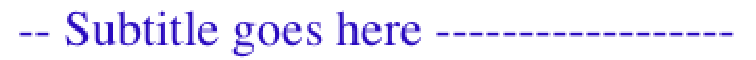
\includegraphics{../images/frontmatter/subtitle.pdf}
\\[13.5cm]
\vspace{0.5cm}
\hspace{6.5cm}\includegraphics{../images/frontmatter/eds.eps}

\newpage
% copyright page 

\thispagestyle{empty}

\small
\noindent \textbf{The Architecture of Open Source Applications, Volume 2} \\
Edited by Amy Brown and Greg Wilson

\vspace{0.15cm}

\noindent
This work is licensed under the Creative Commons Attribution 3.0
Unported license (CC~BY~3.0).  You are free:

\begin{aosaitemize}
  \item to Share---to copy, distribute and transmit the work
  \item to Remix---to adapt the work
\end{aosaitemize}

\noindent
under the following conditions:

\begin{aosaitemize}
  \item Attribution---you must attribute the work in the manner
    specified by the author or licensor (but not in any way that
    suggests that they endorse you or your use of the work).
\end{aosaitemize}

\noindent
with the understanding that:

\begin{aosaitemize}

  \item Waiver---Any of the above conditions can be waived if you get
    permission from the copyright holder.

  \item Public Domain---Where the work or any of its elements is in
    the public domain under applicable law, that status is in no way
    affected by the license.

  \item Other Rights---In no way are any of the following rights
    affected by the license:
    \begin{aosaitemize}

      \item Your fair dealing or fair use rights, or other applicable
        copyright exceptions and limitations;

      \item The author's moral rights;

      \item Rights other persons may have either in the work itself or
        in how the work is used, such as publicity or privacy rights.

    \end{aosaitemize}

  \item Notice---For any reuse or distribution, you must make clear to
    others the license terms of this work. The best way to do this is
    with a link to \url{http://creativecommons.org/licenses/by/3.0/}.

\end{aosaitemize}

\noindent To view a copy of this license, visit
\url{http://creativecommons.org/licenses/by/3.0/} or send a letter to Creative
Commons, 444 Castro Street, Suite 900, Mountain View, California,
94041, USA.\\

\vspace{0.15cm}

\noindent
The full text of this book is available online at \url{http://www.aosabook.org/}.\\
All royalties from its sale will be donated to Amnesty International.\\

\vfill

\noindent Product and company names mentioned herein may be the trademarks of
their respective owners.\\

\vspace{0.15cm}

\noindent While every precaution has been taken in the preparation of this
book, the editors and authors assume no responsibility for errors or omissions,
or for damages resulting from the use of the information contained herein.\\

\vspace{0.15cm}

\noindent Attribution and license for cover photo goes here. FIXME

\vspace{1cm}

\noindent Revision Date: \today \\

\noindent ISBN: New ISBN goes here - FIXME
\normalsize

\newpage
% Dedication page

\thispagestyle{empty}

\vspace*{5cm}
\begin{center}
\hspace{0cm}Dedication goes here. FIXME
\end{center}

\newpage

% Blank page here
\thispagestyle{empty}
\mbox{}    % need to have *something* in here or Latex "helpfully" removes page



\tableofcontents

\begin{aosachapter}{Introduction}{s:intro}{Amy Brown and Greg Wilson}

Mention \cite{bib:aosa1}.

And be sure to thank Google for their support!

\section*{Contributors}

\emph{Andrey Alexeev (nginx)}: FIXME

\emph{Chris AtLee (Firefox Release Engineering)}: FIXME

\emph{Michael Bayer (SQLAlchemy)}: FIXME

\emph{Lukas Blakk (Firefox Release Engineering)}: FIXME

\emph{Amy Brown (editorial)}: Amy worked in the software industry for
ten years before decamping to create a freelance editing and book production
business. She has an underused degree in Math, two small children, a
husband and a cat. She can be found online at \url{http://www.arbrown.ca/}

\emph{Michael Droettboom (matplotlib)}: FIXME

\emph{Elizabeth Flanagan (Yocto)}: FIXME

\emph{Jeff Hardy (Iron Languages)}: FIXME

\emph{Sumana Harihareswara (MediaWiki)}: Sumana is the community manager for
MediaWiki as the volunteer development coordinator for the Wikimedia
Foundation. She previously worked with the GNOME, Empathy, Telepathy,
Miro, and AltLaw projects. Sumana is an advisory board member for the
Ada Initiative, which supports women in open technology and culture.
She lives in New York City. Her personal site is at
\url{http://www.harihareswara.net/}.

\emph{Tim Hunt (Moodle)}: FIXME

\emph{John Hunter (matplotlib)}: John Hunter is a Quantitative Analyst
at TradeLink Securities.  He received his doctorate in neurobiology at
the University of Chicago for experimental and numerical modeling work
on synchronization, and continued his work on synchronization
processes as a postdoc in Neurology working on epilepsy. He left
academia for quantitative finance in 2005.  An avid python programmer
and lecturer in scientific computing in python, he is original author
and lead developer of the scientific visualization package matplotlib.

\emph{Luis Ibanez (ITK)}: Luis has worked for 11 years on the development of
the Insight Toolkit (ITK), an open source library for medical imaging analysis.
Luis is a strong supporter of open access and the revival of reproducibiliy
verification in scientific publishing. Luis has been teaching a course on Open
Source Software Practices at Rensselaer since 2007.

\emph{Mike Kamermans (Processing.js)}: FIXME

\emph{Luke Kanies (Puppet)}: FIXME

\emph{Brad King (ITK)}: FIXME

\emph{Simon Marlow (The Glasgow Haskell Compiler)}: FIXME

\emph{Kate Matsudaira (Scalable Web Architecture and Distributed Systems)}: FIXME

\emph{Jessica McKellar (Twisted)}: FIXME

\emph{John O'Duinn (Firefox Release Engineering)}: FIXME

\emph{Guillaume Paumier (MediaWiki)}: Guillaume is Technical Communications
Manager at the Wikimedia Foundation, the nonprofit  behind Wikipedia
and MediaWiki. A Wikipedia photographer and editor since 2005, Guillaume
is the author of a Wikipedia handbook in French. He also holds an engineering
degree in physics and a Ph.D in microsystems for life sciences. His home online
is at \url{http://guillaumepaumier.com}.

\emph{Benjamin Peterson (PyPy)}: FIXME

\emph{Simon Peyton-Jones (The Glasgow Haskell Compiler)}: FIXME

\emph{Susan Potter (Git)}: Susan is a polyglot software developer with a
penchant for skepticism. She has been designing, developing and deploying
distributed trading services and applications since 1996, recently switching
to building multi-tenant systems for software firms. Susan is a passionate
power user of Git, Linux, and Vim. You can find her tweeting random thoughts
on Erlang, Haskell, Scala, and (of course) Git @SusanPotter\footnote{\url{https://twitter.com/SusanPotter}}.

\emph{Eric Raymond (GPSD)}: FIXME

\emph{Jennifer Ruttan (OSCAR)}: FIXME

\emph{Stan Shebs (GDB)}: Stan has had open source as his day job since
1989, when a colleague at Apple needed a compiler to generate code for
an experimental VM, and GCC 1.31 was conveniently at hand.  After
following up with the oft-disbelieved Mac System 7 port of GCC (it was
the experiment's control case), Stan went to Cygnus Support, where he
maintained GDB for the FSF and helped on many embedded tools projects.
Returning to Apple in 2000, he worked on GCC and GDB for Mac OS X.  A
short time at Mozilla preceded a jump to CodeSourcery, now part of
Mentor Graphics, where he continues to develop new features for GDB.
Stan's professorial tone is explained by his Ph.D. in Computer Science
from the University of Utah.

\emph{Michael Snoyman (Yesod)}: FIXME

\emph{Jeffrey M.\ Squyres (Open MPI)}: Jeff works in the rack server
division at Cisco; he is Cisco's representative to the MPI Forum
standards body and is a chapter author of the MPI-2 standard.  Jeff is
Cisco's core software developer in the open source Open MPI project.
He has worked in the High Performance Computing (HPC) field since his
early graduate-student days in the mid-1990's.  After some active duty
tours in the military, Jeff received his doctorate in Computer Science
and Engineering from the University Notre Dame in 2004.

\emph{Martin Sustrik (ZeroMQ)}: FIXME

\emph{Christopher Svec (FreeRTOS)}: FIXME

\emph{Barry Warsaw (Mailman)}: FIXME

\emph{Greg Wilson (editorial)}: Greg has worked over the past 25 years
in high-performance scientific computing, data visualization, and
computer security, and is the author or editor of several computing
books (including the 2008 Jolt Award winner \emph{Beautiful Code}) and
two books for children.  Greg received a Ph.D.\ in Computer Science
from the University of Edinburgh in 1993.

\emph{Armen Zambrano Gasparnian (Firefox Release Engineering)}: FIXME

\section*{Acknowledgments}

FIXME

\section*{Contributing}

Dozens of volunteers worked hard to create this book, but there is
still a lot to do.  You can help by reporting errors, by helping to
translate the content into other languages, or by describing the
architecture of other open source projects.  Please contact us at
\code{aosa@aosabook.org} if you would like to get involved.

\end{aosachapter}


\mainmatter
\begin{aosachapter}{Scalable Web Architecture and Distributed Systems}{s:distsys}{Kate Matsudaira}

Open Source software has become a fundamental building block for some
of the biggest web sites online. And as those websites have grown,
best practices and guiding principles around these architectures have
emerged. This chapter seeks to cover some of the key things to
consider when designing these types of systems, as well as some of the
building blocks used to achieve these goals.

This chapter is largely focused on web systems, although some of the
material is applicable in other areas of distributed systems as well.

\begin{aosasect1}{Principles of Web Distributed Systems Design}

What exactly does it mean to build and operate a scalable web site or
application? The primitive level is just connecting users with remote
resources via the Internet---and the part that makes it scalable is
that the resources, or access to those resources, are distributed
across multiple servers.

Like most things in life, taking the time to plan ahead can help in
the long run; and since most systems do not start out large,
understanding some of the considerations and tradeoffs behind the big
online sites can result in smarter decisions at the beginning of
smaller web sites. Below are some of the key principles that influence
the design of large-scale web systems:

\begin{aosadescription}

\item{Availability:} The uptime of a website is absolutely critical to
  the reputation and functionality of many companies. For some of the
  larger online retail sites, being unavailable for even minutes can
  result in thousands to millions of dollars in lost revenue; so
  designing their systems to be constantly available and resilient to
  failure is both a fundamental business and technology
  requirement. High availability in distributed systems requires the
  careful consideration of redundancy for key components, rapid
  recovery in the event of partial system failures, and graceful
  degradation when problems occur.

\item{Performance:} Website performance has become an important
  consideration for most online sites. The speed of a website affects
  usage and user satisfaction, as well as search engine rankings, a
  factor that directly correlates to lost revenue and retention. As a
  result creating a system that is optimized for fast responses and
  low latency is key to these large web systems.

\item{Reliability:} A system needs to be reliable, such that a request
  for data will consistently return the same data. In the event the
  data changes or is updated, then that same request should return the
  new data. Users need to know that if something is written to the
  system, or stored, it will persist and can be relied on for future
  retrieval.

\item{Scalability:} When it comes to any large distributed system, its
  size is just one aspect of scale needing to be considered. Just as
  important is the effort required to increase capacity to handle
  greater amounts of load, which is commonly referred to the
  scalability of the system. Scalability can refer to many different
  parameters of the system---how much additional traffic can it
  handle, how easy is it to add more storage capacity, or even how
  many more transactions can be processed.

\item{Manageability:} Similar to scalability, designing a system that
  is easy to operate is another important consideration---in other
  words, the scalability of operations, such as maintenance and
  updates, equates to the manageability of the system . Things to
  consider for manageability are the ease of diagnosis and
  understanding problems when they occur, making updates or
  modifications, and how simple the system is to operate (i.e,. does
  it routinely operate without failure or exceptions).

\item{Cost:} As with any system an important factor is the cost. This
  can include hardware and software costs, but it is also important to
  consider other facets needed to deploy and maintain the
  system. Things like the amount of developer time the system takes to
  build, the amount of operational effort required to run the system,
  and even the amount of training required, should all be
  considered. Cost is the total cost of ownership.

\end{aosadescription}

Each of these principles provides the basis for decisions of
compromise in a distributed web architecture. However, they also can
be at odds with one another, such that achieving one objective comes
at the cost of another. A really basic example: choosing to address
capacity by simply adding more servers (scalability) can come at the
price of manageability (you have to operate an additional server) and
cost (the price of the servers).

When thinking about designing any sort of web application it is
important to consider these key principles, even if it is to
acknowledge that a design may sacrifice one or more of them.

\end{aosasect1}

\begin{aosasect1}{The Basics}

When it comes to system architecture there are a few things to
consider: what are the right pieces, how these pieces fit together,
and what are the right tradeoffs. When it comes to architecture,
investing in scaling before it is needed is generally not a smart
business proposition, however, some forethought into the design can
save substantial time and resources in the future.

This section is focused on some of the core values that are central to
almost all large web applications---\emph{services},
\emph{redundancy}, \emph{partitions}, and \emph{handling
failure}. Each of these values involves choices and compromises,
particularly in the context of the principles described in the
previous section. In order to explain these in detail, though, it is
best to start with an example.

\begin{aosasect2}{Example: Image Hosting Application}

At some point you have probably posted an image online, and for big
sites that host and deliver lots of images, there are certainly
challenges in building an architecture that is cost effective, highly
available, and with low latency (fast retrieval).

Imagine a system where users are able to upload their images to a
central server, and the images can be requested via a web link or
API---just like Flickr or Picasa. For the sake of simplicity, let’s
assume that this application has 2 key parts---the ability to upload
(write) an image to the server, and the ability to query for an
image. While we certainly want the upload to be efficient, we care the
most about having very fast delivery when someone requests an image
(for example, these images could be requested for a web page, or other
application). This is very similar functionality to what a web server,
or Content Delivery Network (CDN) edge server (which is something a
CDN uses to locate content in many locations so the content the users
request are geographically/physically closer, resulting in faster
performance) might provide.

Other important aspects to the system are:

\begin{aosaitemize}

\item There is no limit to the number of images that need to be
  stored, so storage scalability, in terms of image count, needs to be
  considered.

\item There needs to be low latency for image downloads/requests.

\item If a user uploads an image, the image should always be there
  (data reliability for images).

\item The system should be easy to maintain (manageability).

\item Since image hosting doesn’t have high profit margins, the system
  needs to be cost effective

\end{aosaitemize}

Here is a simplified diagram of the functionality:

\Aosafigure{../images/distsys/imageHosting1.jpg}{Simplified Architecture Diagram for Image Hosting Application}{fig.distsys.1}

In this image hosting example, the system must be perceivably fast,
its data stored reliably and all of these attributes highly
scalable. Building a small version of this application would be
trivial, easily hosted on a single server, however, that would not be
interesting for this chapter. Let’s assume that we want to build
something that could (eventually) grow as big as a Flickr, or another
photo sharing site.

\end{aosasect2}

\begin{aosasect2}{Services}

When considering scalable system design, it helps to decouple
functionality and think about each part of the system as its own
service with a clearly defined interface. In practice, systems
designed in this way are said to have a Service Oriented Architecture
(SOA). For these types of systems, each service has its own distinct
functional context and interaction with anything outside of that
context takes place through an abstract interface, typically the
public facing API of another service.

Deconstructing a system into a set of complementary services decouples
the operation of those pieces from one another. This abstraction helps
establish a clear relationship between the service, its underlying
environment, and the consumers of that service. By creating these
clear delineations, it can help isolate problems, but also allows each
piece to scale independently of one another. This sort of
service-oriented design for systems is very similar to object-oriented
design for programming.

In our example, all requests to upload (write) and retrieve images are
being processed by the same server; however as the system needs to
scale it makes sense that these two functions would be broken out into
their own services.

Fast forward and assume that the service is in heavy use; such a
scenario makes it easy to see how longer writes will impact the speed
to read the images (since they two functions will be competing for
shared resources). Depending on the architecture this effect can be
substantial. Even if the upload and download speeds are the same
(which is not true of most IP networks since most are designed for at
least 3:1 download:upload speed), read files will typically be read
from cache, and writes will have to go to disk eventually (and perhaps
written several times in eventually consistent situations)---however,
even if everything is in memory or read from disks (like SSDs),
database writes will almost always be slower than reads\footnote{Pole
  Position, an open source tool for DB benchmarking,
  \url{http://polepos.org/} and results
  \url{http://polepos.sourceforge.net/results/PolePositionClientServer.pdf}.}.

Another potential problem with this design, is that a web server like
Apache or lighttpd, typically can maintain a maximum of simultaneous
connections (defaults are around 500, but can go much higher), and in
high traffic writes can quickly consume all of those. Since reads can
be asynchronous, or take advantage of other performance optimizations
like gzip compression or chunked transfer encoding, the web server can
switch serve reads faster and switch between clients quickly serving
many more requests per second than the max number of connections (with
Apache and max connections set to 500, it is not uncommon to serve
several thousand read requests per second). Writes on the other hand
tend to maintain an open connection for the duration for the upload,
so uploading a 1MB file could take more than 1s on most home networks,
such that same web server could only handle 500 such simultaneous
writes.

Planning for this sort of bottleneck in the future makes a good case
to split out the reads and writes of images into their own
services. This allows us to scale each of them independently (since it
is likely we will always do more reading than writing), but also helps
clarify what is going on at each point. Finally, this separates future
concerns, which would make it easier to troubleshoot and scale a
problem like slow reads.

\aosafigure{../images/distsys/imageHosting2.png}{Splitting out reads and writes.}{fig.distsys.2}

The advantage of this approach is that we are able to solve each
problem independently of one another - we don’t have to worry about
writing new images, and retrieving them in the same context. Each of
these services still leverage the global corpus of images, but both
are free to create their own intermediate results optimal for
achieving performance (for example, queuing up requests, or caching
popular images---more on this below). And from a maintenance and cost
perspective each service can scale independently as needed (which is
great because if they were combined and intermingled one could
inadvertently impact the performance of the other, as in the scenario
discussed above).

Of course the above example can work well when you have two different
endpoints (in fact this is very similar to several cloud storage
providers implementations and Content Delivery Networks). There are
lots of ways to address these types of bottlenecks though, and each
has different tradeoffs.

For example, Filckr solves this read/write issue by federating users
across different shards such that each shard can only handle a set
number of users and as those users grow more shards are added to the
cluster\footnote{Presentation on Flickr’s scaling,
  http://mysqldba.blogspot.com/2008/04/mysql-uc-2007-presentation-file.html}. In
the first example it is easier to scale hardware based on actual usage
(the number of reads and writes across the whole system), whereas
Flickr scales with their user base (but forces the assumption of equal
usage across users so there can be extra capacity). In the former an
outage or issue with one of the services brings down functionality
across the whole system (no one can write files for example), where as
an outage with one of Flickr’s shards will only affect those users. In
the first example it is easier to perform operations across the whole
dataset, for example updating the write service to include new
metadata or searching across all image metadata, where as with the
Flickr architecture each shard would need to be updated or searched
(or a search service would need to be created to collate that
metadata---which is in fact what they do.

When it comes to these systems there is no right answer, but it helps
to go back to the principles at the start of this chapter, determine
the system needs (heavy reads or writes or both, level of concurrency,
queries across the data set, ranges, sorts, etc.), benchmark different
alternatives, understand how it will fail, and then have a solid plan
for when that happens.

\end{aosasect2}

\begin{aosasect2}{Redundancy}

In order to handle failure gracefully a web architecture must have
redundancy of its services and data. For example, if there is only one
copy of a file stored on a single server then losing that server also
means losing that file. Losing data is seldom a good thing, and a
common way of handling it is to create multiple, or redundant, copies.

This same principle also applies to services. If there is a core piece
of functionality for an application, ensuring that multiple copies or
versions are running simultaneously can secure against the failure of
a single node.

Creating redundancy in a system can remove single points of failure,
and provide a backup or spare functionality if needed in a crisis. For
example, if there are two instances of the same service running in
production, and one fails or degrades, the system can \emph{failover}
to the healthy copy. When it comes to failover, this can happen
automatically or require manual intervention.

Another key part of service redundancy, is creating a \emph{shared
  nothing architecture}. With this architecture, each node is able to
operate independently of one another and there is no central ``brain''
managing state or coordinating activities for the other nodes. This
helps a lot with scalability since new nodes can be added without
special conditions or knowledge. However, and most importantly, there
is no single point of failure in these systems, so they are much more
resilient to failure.

For example, in our image server application, all images would have
redundant copies on another piece of hardware somewhere (ideally in a
different geographic location in the event of a catastrophe like an
earthquake or fire in the data center), and the services to access the
images would be redundant copies, all potentially servicing requests
(load balancers are a great way to make this possible, but there is
more on that below).

\aosafigure{../images/distsys/imageHosting3.png}{Image hosting application with redundancy}{fig.distsys.3}

\end{aosasect2}

\begin{aosasect2}{Partitions}

There may be very large data sets that are unable to fit on a single
server. It may also be the case that an operation requires too many
computing resources, diminishing performance, and therefore makes it
necessary to add capacity. In either case you have two choices: scale
vertically or horizontally.

Scaling vertically means adding more resources to an individual
server. So for a very large data set, this might mean adding more (or
bigger) hard drives so a single server can contain its entirety. In
the case of the compute operation, this could mean moving the
computation to a bigger server with a faster CPU or more memory. In
each case vertical scaling is accomplished by making the individual
resource better and capable of handling more on its own.

To scale horizontally, on the other hand, is to add more nodes. In the
case of the data, this might be a second server to store the
additional parts of the data set; and for the computing resource it
would mean splitting the operation or load across some additional
nodes. To take full advantage of horizontal scaling, the system should
include it as an intrinsic design principle of the system
architecture, otherwise it can be quite cumbersome to modify and
separate out the context to make this possible.

And when it comes to horizontally scaling, one of the more common
techniques is to break-up your services into partitions (some may also
refer to these pieces as shards). The partitions can be federated such
that each logical set of functionality is separate---this could be
done by geographic boundaries, or another criteria like free versus
paying users. The advantage of these schemes is to provide a service
or data store with added capacity.

In our image server example, it is possible that the single file
server used to store images could be replaced by multiple file
servers, each containing its own unique set of images. Such an
architecture would allow the system to fill each file server with
images, adding additional servers as the disks become full. This sort
of design would require a naming scheme that tied an image’s filename
with the server containing it. An image’s name could be formed from a
consistent hashing scheme mapped across the servers. Or alternatively,
each image could be assigned an incremental ID, so that when a client
makes a request for an image, the image retrieval service only needs
to maintain the range of IDs that are mapped to each of the servers
(like an index).

\aosafigure{../images/distsys/imageHosting4.png}{FIXME}{fig.distsys.4}

Of course there are challenges distributing data or functionality
across multiple servers. One of the key issues is \emph{data
  locality}; in distributed systems any time the data is closer to the
operation or point of computation, the better performance of the
system. Therefore it is potentially problematic to have the data
spread across multiple servers, as any time it is needed it may not be
local, forcing the servers to perform a costly fetch of the required
information across the network.

Another potential issue comes in the form of
\emph{inconsistency}. When there are different services reading and
writing from a shared resource (potentially another service or data
store) there is the chance for race conditions, where some data was
supposed to be updated, but the read happens prior to the update---and
in those cases the data is inconsistent. For example, in the image
hosting scenario, a race condition could occur if one client sent a
request to update the dog image with a new title (changing it from
``Dog'' to ``Gizmo''), but at the same time another client was reading
the image. In that circumstance it is unclear which title (``Dog'' or
``Gizmo'') would be the one received by the second client.

There are certainly some obstacles associated with partitioning data,
but partitioning allows each problem to be split (by data, load, usage
patterns, etc.) into manageable chunks. This can help with scalability
and manageability, but is not without risk.

There are lots of ways to mitigate risk and handle failures, however,
in the interest of brevity they are not covered in this chapter. If
you are interested in reading more, you can check out my blog post
on fault tolerance and monitoring\footnote{\url{http://katemats.com/2011/11/13/distributed-systems-basics-handling-failure-fault-tolerance-and-monitoring/}}.

\end{aosasect2}

\end{aosasect1}

\begin{aosasect1}{The Building Blocks of Fast and Scalable Data Access}

Having covered some of the core considerations in designing
distributed systems, let’s now talk about the hard part---scaling
access to the data.

Most simple web applications (for example, LAMP stack applications)
often look something like the following:

\aosafigure{../images/simpleWeb.png}{Simple web applications}{fig.distsys.5}

As they grow, there are two main challenges---scaling access to the
app server and to the database. In a highly scalable application
design, the app (or web) server is typically minimized and often
embodies a shared nothing architecture. This makes the app server
layer of the system horizontally scalable. As a result of this design,
the heavy lifting is pushed down the stack to the database server and
supporting services; it’s at this layer where the real scaling and
performance challenges come into play.

The rest of this chapter is devoted to some of the more common
strategies and methods for making these types of services fast and
scalable by providing fast access to your data.

Most systems can be oversimplified to this:

\aosafigure{../images/distsys/overSimpleWeb.png}{Oversimplified web applications.}{fig.distsys.6}

This is a great place to start. If you have a lot of data, you want
fast and easy access, like a secret stash of candy in the top drawer
of your desk. Though overly simplified, the previous statement hints
at two hard problems: scalability of storage and fast access of data.

For the sake of this section, let’s assume you have many terabytes of
data (TB) and you want to allow users to access small portions (KBs)
of that data at random. This is similar to locating an image file
somewhere on the larger file server in the image application example.

\aosafigure{../images/distsys/accessingData.png}{Accessing specific data}{fig.distsys.7}

This is particularly challenging because it can be very costly to load
TBs of data into memory---this directly translates to disk IO. Reading
from disk is many times slower than from memory---memory access is
almost as fast as Chuck Norris, whereas disk access is slower than the
line at the DMV; and this speed difference really adds up for large
data sets (in real numbers memory access is as little as 6 times
faster for sequential reads, or 100,000 times faster for random
reads\footnote{The Pathologies of Big Data,
  \url{http://queue.acm.org/detail.cfm?id=1563874}.} than reading from
disk). Moreover, even with unique ID’s---solving the problem of
knowing where to find that little bit of data can be an arduous
task. It is like searching for a needle in a really big haystack, or
trying to get that last Jolly Rancher in your candy stash without
looking.

Thankfully there are many options that you can employ to make this
easier; and three of the more important ones are caches, proxies,
indexes and load balancers. The rest of this section goes through each
of these concepts and discusses how each can be used to make data
access a lot faster.

\begin{aosasect2}{Caches}

Caches take advantage of the locality of reference
principle---recently requested data is likely to be requested
again. They are used in almost every layer of computing, such as your
hardware, the operating system, web browsers, web applications and
more. A cache is like short-term memory; it has a limited amount of
space, but is typically faster than the original data source, and
contains the most recently accessed items. Caches can exist at all
levels in your architecture, but it's often found at the level nearest
to the frontend, where it is implemented to quickly return data
without taxing the downstream levels

How can a cache be used to make your data access faster in our API
example?

In this case, there are a couple of places you can insert a cache:

One option is to insert a cache on your request layer node:

\aosafigure{../images/distsys/cache.png}{Inserting a cache on your request layer node}{fig.distsys.8}

Placing a cache directly on a request layer node enables the local
storage of response data. Each time a request was made to the service,
the node would quickly return local, cached data if it existed. If it
were not there, the request node would query the data from disk. The
cache on one request layer node could also be located both in memory
(which is very fast) and on the node’s local disk (faster than going
to network storage).

What happens when you expand this to many nodes?

\aosafigure{../images/distsys/multipleCaches.png}{Multiple caches}{fig.distsys.9}

If the request layer were expanded to multiple nodes, it’s still quite
possible to have it each host its own cache. However, if your load
balancer randomly distributes requests across the nodes, the same
request will go to different nodes, thus increasing cache misses. Two
choices for overcoming this hurdle are global caches and distributed
caches. Read on to learn more!

\end{aosasect2}

\begin{aosasect2}{Global Cache}

A global cache is just as it sounds---all the nodes use a single cache
space. This involves adding a server, or file store of some sort;
faster than your original store and accessible by all the request
layer nodes. Each of the request nodes queries the cache in the same
way it would a local one. This kind of caching scheme can get a bit
complicated because it is very easy to overwhelm a single cache as the
number of clients and request increase, but is very effective in some
architectures (particularly ones with specialized hardware that make
this global cache very fast, or have a fixed dataset that needs to be
cached).

\aosafigure{../images/distsys/globalCache1.png}{Global cache where cache is responsible for retrieval}{fig.distsys.10}

\aosafigure{../images/distsys/globalCache2.png}{Global cache where request nodes are responsible for retrieval}{fig.distsys.11}

There are two common forms of global caches depicted in the
diagrams. In the first diagram, when a cached response is not found in
the cache, the cache itself becomes responsible for retrieving the
missing piece of data from the underlying store; and in the second it
is the responsibility of request nodes to retrieve any data that is
not found in the cache.

The majority of applications leveraging global caches tend to use the
first type---the cache itself manages eviction and fetching data (to
prevent a flood of requests for the same data from the
clients). However there are some exceptions where the second
implementation makes more sense. For example, if the cache is being
used for very large files, a low cache hit percentage would cause the
cache buffer to become overwhelmed with cache misses; in this
situation it helps to have a large percentage of the total data set
(or hot data set) in the cache. Another example, is in a design where
the files stored in the cache are static and shouldn’t be evicted;
this could be because of application requirements around that data
latency---certain pieces of data need to be very fast for really large
data sets where the application logic understands the eviction
strategy or hot spots better than the cache.

\end{aosasect2}

\begin{aosasect2}{Distributed Cache}

In a distributed cache, each of its nodes own part of the cached data,
so like a refrigerator acts as a cache to the grocery store, a
distributed cache is like putting your food in several locations---you
cupboards, fridge and lunch box---all our convenient locations for
snacks without a trip to the store. Typically the cache is divided up
using a consistent hashing function, such that if a request node is
looking for a certain piece of data it can quickly know where to look
within the distributed cache to determine if that data is
available. In this case, each node has a small piece of the cache, and
will then send a request to another node for the data, before going to
the origin. Therefore, one of the advantages of a distributed cache is
the increased cache space that can be had just by adding additional
nodes to the request pool.

A disadvantage of distributed caching is remedying a missing
node. Some distributed caches get around this by storing multiple
copies of the data on different nodes, however you can imagine how
this logic can get complicated quickly, especially when you add or
remove nodes from the request layer. Although, even if a node
disappears and part of the cache is lost, the requests will just pull
from the origin---so it isn’t necessarily catastrophic!

\aosafigure{../images/distsys/distributedCaching.png}{FIXME}{fig.distsys.12}

The great thing about caches is that they usually make things much
faster (implemented correctly of course!) The methodology you choose
just allows you to make it faster for even more requests. However all
this caching comes at the cost of having to maintain additional
storage space, typically in the form of expensive memory; nothing is
free. Caches are wonderful for making things generally faster, but
moreover provide system functionality under high load conditions when
otherwise there would be complete service degradation.

One example of a popular open source cache is
Memcached\footnote{\url{http://memcached.org/}} (which can work both
as a local cache and distributed cache), however there are many other
options (including many language or framework specific options).

Memcached is used in many large web sites, and even though it can be
very powerful, it is simply an in-memory key value store, optimized
for arbitrary data storage and fast lookups (O(1)).

For example, Facebook uses several different types of caching to
obtain their site performance\footnote{Facebook caching and
  performance, \url{http://sizzo.org/talks/}.}. They use \$GLOBALS and
APC caching at the language level (PHP) which helps make intermediate
function calls and results much faster at the language level (provided
in php at the cost of a function call). Most languages have these
types of libraries to improve web page performance and should almost
always be implemented/enabled. Then they use a global cache that is
distributed across many servers\footnote{Scaling memcached at
  Facebook,
  \url{http://www.facebook.com/note.php?note_id=39391378919}.}, such
that one function call accessing the cache could make many requests in
parallel for data stored on different Memcached servers. This allows
them to get much higher performance and throughput for their user
profile data, and have one central place to update data (which is
important, since cache invalidation and maintaining consistency can be
challenging when you are running thousands of servers).

Now let’s talk about what to do when the data isn’t in the cache{\ldots}

\end{aosasect2}

\begin{aosasect2}{Proxies}

At a basic level, a proxy server is an intermediary piece of
hardware/software that receives requests from clients and relays them
to the backend origin servers. Typically, proxies are used to filter
requests, log requests, or sometimes transform requests (by
adding/removing headers, encrypting/decrypting, or compression).

\aosafigure{../images/distsys/proxies.png}{Proxy server}{fig.distsys.13}

Proxies are also immensely helpful when coordinating requests from
multiple servers, providing opportunities to optimize request traffic
from a system-wide perspective. One way to use a proxy to speed up
data access is to collapse the same (or similar) requests together
into one request, and then return the single result to the requesting
clients. This is known as collapsed forwarding.

Imagine there is a request for the same data (let’s call it littleB)
across several nodes, and that piece of data is not in the cache. If
that request is routed thought the proxy, then all of those requests
can be collapsed into one; which means we only have to read littleB
off disk once. There is some cost associated to this design, since
each request can have slightly higher latency, and some requests may
be slightly delayed to be grouped with similar ones. But this will
improve performance in high load situations, particularly when that
same data is requested over and over. This is similar to a cache, but
instead of storing the data/document like a cache, it is optimizing
the requests or calls for those documents and acting as a proxy for
those clients. In a LAN proxy for example, the clients do not need
their own IPs to connect to the Internet, and the LAN will collapse
calls from the clients for the same content. It is easy to get
confused here though, since many proxies are also caches (as it is a
very logical place to put a cache), but not all caches act as proxies.

\aosafigure{../images/distsys/collapseRequests.png}{Using a proxy server to collapse requests}{fig.distsys.14}

Another great way to use the proxy is to not just collapse requests
for the same data, but also to collapse requests for data that is
spatially close together in the origin store (consecutively on disk);
employing such a strategy maximizes data locality for the requests,
which can result in decreased request latency. For example, let’s say
a bunch of nodes request parts of B---partB1, partB2, etc. We can
setup our proxy to recognize the spatial locality of the individual
requests, collapsing them into a single request and returning only
bigB, greatly minimizing the reads from the data origin. This can make
a really big difference in request time when you are randomly
accessing across TBs of data! Proxies are especially helpful under
high load situations, or when you have limited caching since they
essentially can batch several requests into one.

\aosafigure{../images/distsys/collapseRequestsSpatial.png}{FIXME}{fig.distsys.15}

It is worth noting that you can use proxies and caches together, but
generally it is best to put the cache in front of the proxy,
similarly, it is best to let the faster runners start first in a
crowded marathon race. This is because the cache is serving data from
memory, it is very fast, and doesn’t mind multiple requests for the
same result. But if the cache was located on the other side of the
proxy server, then there would be additional latency with every
request before the cache, and this could hinder performance.

If you are looking at adding a proxy to your systems, there are many
options to
consider\footnote{\url{http://en.wikipedia.org/wiki/Web_accelerator}};
Squid\footnote{\url{http://www.squid-cache.org/}} and
Varnish\footnote{\url{https://www.varnish-cache.org/}} have both been
road tested and are widely used in many production web sites. These
proxy solutions offer many optimizations to make the most of
client-server communication. Installing one of these as a reverse
proxy (explained in the load balancer section below) at the web server
layer can improve web server performance considerably, reducing the
amount of work required to handle incoming client requests.

\end{aosasect2}

\begin{aosasect2}{Indexes}

Using an index to access your data quickly is a well-known strategy
for optimizing data access performance, and probably the most well
known when it comes to databases. An index makes the trade-offs of
increased storage overhead and slower writes (since you must both
write the data and update the index) for the benefit of faster reads.

Just as to a traditional relational data store, you can also apply
this concept to larger data sets. The trick with indexes is you must
carefully consider how users will access your data. In the case of
data sets that are many TBs large, with very small payloads
(e.g. 1kb), indexes are a necessity for optimizing data
access. Finding a small payload in such a large data set can be a real
challenge since you can’t possibly iterate over that much data in any
reasonable time. Furthermore, it is very likely that such a large data
set is spread over several (or many!) physical devices---this means
you need some way to find the correct physical location of the desired
data.

What is the best way to do this? Enter indexes!

An index can be used like a table of contents that directs you to the
right location where your data lives. These indexes provide a fast
lookup directing you to the locality of the data; just like the card
catalog in a library. For example, let’s say you are looking for a
piece of data, part 2 of B---how will you know where to find it? If
you have an index that is sorted by data type---say data A, B, C---it
would tell you the location of data B at the origin. Then, you just
have to seek to that location and read the part of B you want.

\aosafigure{../images/indexes.jpg}{Indexes}{fig.distsys.16}

These indexes are often stored in memory, or somewhere very local to
the incoming client request. Berkeley DBs (BDBs) and other tree like
data structures are commonly used to store data in ordered lists,
ideal for access with an index.

Often times, there are many layers of indexes that serve as a
map---moving you from one location to the next, and so forth---until
you get the specific piece of data you want.

\aosafigure{../images/distsys/multipleIndexes.jpg}{Many layers of indexes}{fig.distsys.17}

Indexes can also be used to create several different views of the same
data. For large data sets, this is a great way to define different
filters and sorts without resorting to creating many additional copies
of the data.

For example imagine that the image hosting system from earlier is
actually hosting images of book pages, and the service allows client
queries across of the text in those images. Searching all the book
content about a topic, in the same way search engines allow one to
search html content. In this case all those book images take many,
many servers to store the files, and finding one page to render to the
user can be a bit involved. First, there are the inverse indices to
query for arbitrary words and word tuples need to be easily
accessible, then there is the challenge of navigating to the exact
page and location within that book (and retrieving the right image for
the results). So in this case the inverted index would map to a
location (such as book B), and then B may contain an index with all
the words, locations and number of occurrences in each part.

An inverted index, which could represent Index1 in the diagram above,
might look something like the following---each word or tuple of words
provide an index of what books contain them.

\begin{tabular}{ll}
Word(s) & Book(s) \\
being awesome & Book B, Book C, Book D \\
always & Book C, Book F \\
believe & Book B \\
\end{tabular}

The intermediate index would look similar but would contain just the
words, location, and information for book B. This nested index
architecture allows each of these indices to take up less space, than
if all of that info had to be stored into one big inverted index.

And this is key in large-scale systems, because even compressed these
indices can get quite big and expensive to store. In this system if we
assume we have a lot of the books in the world
100,000,000\footnote{Inside Google Books blog post,
  \url{http://booksearch.blogspot.com/2010/08/books-of-world-stand-up-and-be-counted.html}.}
and that each book is only 10 pages long (to make the math easier),
with 250 words per page, an average of 5 characters per word---that
means there 250 billion words, and if each character takes 8 bits (or
1 byte, even though some characters are 2 bytes), or 5 bytes per word,
then just that data alone is over a terabyte (!) of storage---for one
index containing each word once. So creating indices that have a lot
of other information, like tuples of words, locations for the data,
and count of occurrences can add up very quickly.

By creating these intermediate indices and representing the data in
smaller sections it makes these big data problems tractable. Data can
be spread across many servers and still accessed quickly. Indices are
a cornerstone of information retrieval and the basis for today’s
modern search engines. Of course, this section only scratched the
surface, and there is a lot of research being done on how to make
indices smaller and take up less space, faster, contain more
information (like relevancy), and update seamlessly (there are some
manageability challenges with race conditions, and the sheer number of
updates required to add a new book or change one of the existing
books, particularly in the event where relevancy or scoring is
involved).

Being able to find your data quickly and easily is important; indexes
are an effective and simple tool to achieve this.

\end{aosasect2}

\begin{aosasect2}{Load Balancers}

Finally another critical piece of any distributed system are load
balancers (LBs). LBs are a principal part of any architecture as their
role is to distribute load across a set of nodes responsible for
servicing requests. This allows multiple nodes to transparently
service the same function in a system. Their main purpose is to handle
a lot of simultaneous connections and route those connections to one
of the request nodes---allowing the system to scale to service more
requests by just adding nodes.

\aosafigure{../images/distsys/loadBalancer.png}{Load balancer}{fig.distsys.18}

There are many different algorithms that can be used to service
requests, including picking a random node, round robin
(http://en.wikipedia.org/wiki/Round-robin), or even selecting the node
based on certain criteria---such as memory or CPU utilization. LBs can
be implemented as software or hardware appliances. One open source
software load balancer that has received wide adoption is
HAProxy\footnote{\url{http://haproxy.1wt.eu/}}.

In a distributed system, load balancers are often found at the very
front of the system such that all incoming requests are routed
accordingly. In a complex distributed system, it is not uncommon for a
request to be routed to multiple load balancers as shown below.

\aosafigure{../images/distsys/multipleLoadBalancers.png}{Multiple load balancers}{fig.distsys.19}

Similar to proxies, some load balancers can also route a request
differently depending on the type of request (technically these are
also known as reverse proxies).

One of the challenges with load balancers is managing user session
specific data. In an ecommerce site when you only have one client, it
is very easy to allow users to put things in their shopping cart and
persist those contents between visits (which is important, because it
is much more likely you will sell the product if it is still in the
user’s cart when they return). However, if a user is routed to one
node for a session, and then a different node on their next visit,
there can be inconsistencies since the new node may be missing that
user’s cart contents (Wouldn’t you be upset if you put a 6 pack of
Mountain Dew in your cart and then came back and it was empty? Of
course, with this example it is highly unlikely you would ever forget
about your Mountain Dew so it might be less of an issue.). One way
around this can be to make sessions sticky so that the user is always
routed to the same node, but then it is very hard to take advantage of
some reliability features like automatic failover. In this case, the
user’s shopping cart would always have the contents, but if their
sticky node became unavailable there would need to be a special case
and the assumption of the contents being there would no longer be
valid (although hopefully this assumption wouldn’t be built into the
application :) ). Of course this problem can be solved using other
strategies and tools in this chapter, like services, and many not
covered (like browser caches, cookies, and url rewriting).

If a system only has a couple of a nodes, systems like round robin DNS
may make more sense since load balancers can be expensive and add an
unneeded layer of complexity. Of course in larger systems there are
all sorts of different scheduling and load balancing algorithms,
including simple ones like random choice or round robin, and more
sophisticated mechanisms that take things like utilization and
capacity into consideration. All of these algorithms allow traffic and
requests to be distributed, and can provide helpful reliability tools
like automatic failover, or automatic removal of a bad node (such as
when it becomes unresponsive). Although these advanced features can
make problem diagnosis cumbersome. For example, when it comes to high
load situations, load balancers will remove nodes that may be slow or
timing out (because of too many requests) and that only exacerbates
the situation on the other nodes. In these cases extensive monitoring
is important, because overall system traffic and throughput may look
like it is decreasing (since the nodes are serving less requests) but
the individual nodes become maxed out.

LBs are an easy way to allow you to expand system capacity and like
the other techniques in this article, play an essential role in
distributed system architecture. Load balancers also provide a
critical function of being able to test the health of a node, such
that if a node is unresponsive or over loaded, it can be removed from
the pool handling requests---taking advantage of the redundancy of
different nodes in your system.

\end{aosasect2}

\begin{aosasect2}{Queues}

So far we have covered a lot of ways to read data, quickly, but
another important part of scaling the data layer is effective
management of writes. When systems are simple, having minimal
processing loads and small databases, writes can be predictably fast,
however in more complex systems writes can take an almost
non-deterministically long time (for example, data may have to be
written several places on different servers or indexes, or the system
could just be under high load). In the cases where writes, or any task
for that matter, may take a long time, achieving performance and
availability requires building asynchrony into the system; and a
common way to do that is with queues.

Imagine a system where each client is requesting a task to be remotely
serviced. Each of these clients sends their request to the server,
where the server completes the tasks as quickly as possible and
returns the results to their respective clients. In small systems
where one server (or logical service) can service incoming clients
just as fast as they come in this sort of situation should work just
fine. However, when the server receives more requests than it can
handle, then each client is forced to wait for the other clients’
requests to complete before a response can be generated. This is an
example of a synchronous request and depicted below.

\aosafigure{../images/distsys/synchronousRequest.png}{Synchronous request}{fig.distsys.20}

This kind of synchronous behavior can severely degrade client
performance; the client is forced to wait, effectively performing zero
work until its request can be answered. Adding additional servers to
address system load does not solve the problem either, even with
effective load balancing in place it is extremely difficult to ensure
the even and fair distribution of work required to maximize client
performance. Further, if the server handling requests is unavailable,
or fails, then the clients upstream will also fail. Solving this
problem effectively requires abstraction between the client’s request
and the actual work performed to service it.

Enter queues. A queue is as simple as it sounds, a task comes in, is
added to the queue and then workers pick up the next task as they have
the capacity to process it. These tasks could represent writes to a
database, or something as complex as generating a thumbnail preview
image for a document. When a client submits task requests to a queue
they are no longer forced to wait for the results, instead they need
only acknowledgement that the request was properly received. This
acknowledgement can later serve as a reference for the results of the
work when the client requires it.

Queues enable clients to work in an asynchronous manner, providing a
strategic abstraction of a client’s request and its response. On the
other hand, in a synchronous system, there is no differentiation
between request and reply, and therefore cannot be managed
separately. In an asynchronous system the client requests a task, the
service responds with a message acknowledging the task was received,
and then the client can periodically check the status of the task,
only requesting the result once it has completed. While the client is
waiting for an asynchronous request to be completed it is free to
perform other work, even making asynchronous requests of other
services. The latter is an example of how queues and messages are
leveraged in distributed systems.

Queues also provide some protection from service outages and
failures. For instance, it is quite easy to create a highly robust
queue that can retry service requests having failed to due transient
server failures. It is more preferable utilizing a queue to enforce
quality-of-service guarantees than exposing clients directly to
intermittent service outages requiring complicated and
often-inconsistent client-side error handling.

\aosafigure{../images/distsys/queues.png}{Using queues to manage requests}{fig.distsys.21}

Queues are fundamental in managing distributed communication between
different parts of any large-scale distributed system, and there are
lots of ways to implement them. There are quite a few open source
queues like RabbitMQ\footnote{\url{http://www.rabbitmq.com/}},
ActiveMQ\footnote{\url{http://activemq.apache.org/}},
BeanstalkD\footnote{\url{http://kr.github.com/beanstalkd/}}, but some
also use services like
Zookeeper\footnote{\url{http://zookeeper.apache.org/}}, or even data
stores like Redis\footnote{\url{http://redis.io/}}.

\end{aosasect2}

\end{aosasect1}

\begin{aosasect1}{Conclusion}

Designing efficient systems with fast access to lots of data is
exciting, and there are lots of great tools that enable all kinds of
new applications. This chapter covered just a few examples, barely
scratching the surface, but there are many more—and there will only
continue to be more innovation in the space.

\end{aosasect1}

\end{aosachapter}

\begin{aosachapter}{Firefox Release Engineering}{s:ffreleng}{Chris AtLee, Lukas Blakk, John O'Duinn, and Armen Zambrano Gasparnian}

Recently, the Mozilla Release Engineering team has made numerous advances
in release automation for Firefox. We have
reduced the requirements for human involvement during signing and sending
notices to stakeholders, and have automated
many other small manual steps, because each manual step in the process is an
opportunity for human error. While what we have now isn't perfect,
we're always striving to streamline and automate our release
process. Our final goal is to be able to push a button and walk away;
minimal human intervention will eliminate many of the
headaches and do-overs we experienced with our older part-manual,
part-automated release processes. In this chapter, we will explore and
explain the scripts and infrastructure decisions that comprise
the complete Firefox rapid release system, as of Firefox 10.

You'll follow the system from the perspective of a release-worthy
Mercurial changeset as it is turned into a release candidate---and
then a public release---available to over 450 million daily users
worldwide.  We'll start with builds and code signing, then customized
partner and localization repacks, the QA process, and how we generate
updates for every supported version, platform and localization. Each of
these steps must be completed before the release can be pushed out to
Mozilla Community's network of mirrors which provide the downloads to
our users.

We'll look at some of the decisions that have been made to
improve this process; for example, our sanity-checking script that helps
eliminate much of what used to be vulnerable to human error; our
automated signing script; our integration of mobile releases into the
desktop release process; patcher, where updates are created; and AUS (Application Update Service), where updates are
served to our users across multiple versions of the software.

This chapter describes the mechanics of how we generate release builds
for Firefox. Most of this chapter details the significant
steps that occur in a release process once the builds start, but
there is also plenty of complex cross-group communication to deal
with before Release Engineering even starts to generate release
builds, so let's start there.

\begin{aosasect1}{Look \code{N} Ways Before You Start a Release}

\aosafigure[100pt]{../images/ffreleng/gotobuild.png}{Getting from code to ``Go to build''}{fig.ffreleng.getting}

When we started on the project to improve Mozilla's release process,
we began with the premise that the more popular Firefox became, the
more users we would have, and the more attractive a target Firefox would
become to blackhat hackers looking for security vulnerabilities to
exploit. Also, the more popular Firefox became, the more users we
would have to protect from a newly discovered security vulnerability,
so the more important it would be to be able to deliver a security fix as quickly
as possible. We even have a term for this: a ``chemspill''
release\footnote{Short for ``chemical spill''.}. Instead of being surprised by the occasional need for a
chemspill release in between our regularly scheduled releases, we
decided to plan as if every release could be a chemspill release, and
designed our release automation accordingly.

This mindset has three important side-effects:

\begin{aosaenumerate}

\item We do a postmortem after \emph{every} release, and look to see
  where things could be made smoother, easier, and faster next
  time. If at all possible, we find and fix at least one thing,
  no matter how small, immediately---before the next release. This constant
  polishing of our release automation means we're always looking for
  new ways to rely on less human involvement while also improving
  robustness and turnaround time. A lot of effort is spent
  making our tools and processes bulletproof so that ``rare'' events
  like network hiccups, disk space issues or typos made by real live
  humans are caught and handled as early as possible.  Even though
  we're already fast enough for regular, non-chemspill releases, we
  want to reduce the risk of any human error in a future
  release. This is especially true in a chemspill release.

\item When we do have a chemspill release, the more robust the
  release automation, the less stressed the humans in Release
  Engineering are. We're used to the idea of going as fast as
  possible with calm precision, and we've built tools to do
  this as safely and robustly as we know how. Less stress means more
  calm and precise work within a well-rehearsed process, which in turn
  helps chemspill releases go smoothly.

\item We created a Mozilla-wide ``go to build'' process. When doing a
  regular (non-chemspill) release, it's possible to have everyone look
  through the same bug triage queries, see clearly when
  the last fix was landed and tested successfully, and reach consensus on
  when to start builds. However, in a chemspill release---where
  minutes matter---keeping track of all the details of the issue as well as
  following up bug confirmations and fixes gets very tricky very
  quickly.  To reduce complexity and the risk of mistakes, Mozilla
  now has a full-time person 
  to track the readiness of the code for a ``go to build''
  decision. Changing processes
  during a chemspill is risky, so in order to make sure everyone
  is familiar with the process when minutes matter, we use this
  same process for chemspill and regular releases.

\end{aosaenumerate}

%% FIXME: Don't forget to check this image in the printed proof. --ARB
\aosafigure{../images/ffreleng/timeline.png}{Complete release timeline, using a chemspill as example}{fig.ffreleng.timeline}

\end{aosasect1}

\begin{aosasect1}{"Go to Build"}

\begin{aosasect2}{Who Can Send the ``Go to Build''?}

Before the start of the release, one person is designated to assume
responsibility for coordinating the entire release. This person needs to 
attend triage meetings, understand the
background context on all the work being landed, referee bug severity
disputes fairly, approve landing of late-breaking changes, and make
tough back-out decisions.  Additionally, on the actual release day
this person is on point for all communications with the different
groups (developers, QA, Release Engineering, website developers, PR,
marketing, etc.).

Different companies use different titles for this role. Some titles we've heard 
include Release Manager, Release Engineer, Program Manager, Project 
Manager, Product Manager, Product Czar, Release
Driver. In this chapter, we will use the term ``Release Coordinator''
as we feel it most clearly defines the role in our process as described above. 
The important point here is that the role, and the final authority of the role, is
clearly understood by everyone before the release starts, regardless 
of their background or previous work experiences elsewhere. In the 
heat of a release day, it is important tnat everyone knows to abide by, and trust, 
the coordination decisions that this person makes. 

The Release Coordinator is the only person outside of Release
Engineering who is authorized to send ``stop builds'' emails if a
show-stopper problem is discovered. Any reports of
suspected show-stopper problems are redirected to the Release
Coordinator, who will evaluate, make the final go/no-go decision and
communicate that decision to everyone in a timely manner. In the heat 
of the moment of a release day, we all have to abide by, and trust, the 
coordination decisions that this person makes. 

\end{aosasect2}

\begin{aosasect2}{How to Send the ``Go to Build''?}

Early experiments with sending ``go to build'' in IRC channels or
verbally over the phone led to misunderstandings,
occasionally causing problems for the release in progress. Therefore,
we now require that the ``go to build'' signal for every release is
done by email, to a mailing list that includes everyone across all
groups involved in release processes. The subject of the email
includes ``go to build'' and the explicit product name and version
number; for example:

\begin{verbatim}
go to build Firefox 6.0.1
\end{verbatim}

Similarly, if a problem is found in the release, the Release
Coordinator will send a new ``all stop'' email to the same mailing list,
with a new subject line. We found that it was not sufficient to just hit reply
on the most recent email about the release; email threading in some
email clients caused some people to not notice the ``all stop'' email if
it was way down a long and unrelated thread.

\end{aosasect2}

\begin{aosasect2}{What Is In the ``Go to Build'' Email?}

\begin{aosaenumerate}

\item The exact code to be used in the build; ideally, the URL to the
specific change in the source code repository that the release builds are
to be created from.

  \begin{aosaenumerate2}

    \item Instructions like ``use the latest code'' are never acceptable; in one
      release, after the ``go to build'' email was sent and before
      builds started, a well-intentioned developer landed a change,
      without approval, in the wrong branch. The release included that
      unwanted change in the builds. Thankfully the mistake was
      caught before we shipped, but we did have to delay the release 
      while we did a full stop and rebuilt everything.

    \item In a time-based version control system like CVS, be fully
      explicit about the exact time to use; give the time down to seconds,
      and specify timezone. In one release, when Firefox was still
      based on CVS, the Release Coordinator specified the cutoff time
      to be used for the builds but did not give the timezone. By the
      time Release Engineering noticed the missing timezone info, the
      Release Coordinator was asleep. Release
      Engineering correctly guessed that the intent was local time (in
      California), but in a late-night mixup over PDT instead of PST
      we ended up missing the last critical bug fix. This was caught
      by QA before we shipped, but we had to stop builds and
      start the build over using the correct cutoff time.

    \end{aosaenumerate2}

\item A clear sense of the urgency for this particular release.  While
  it sounds obvious, it is important when handling some important edge
  cases, so here is a quick summary:

  \begin{aosaenumerate2}

    \item Some releases are ``routine'', and can be worked on in
      normal working hours. They are a pre-scheduled release, they are
      on schedule, and there is no emergency. Of course, all release
      builds need to be created in a timely manner, but there is no
      need for release engineers to pull all-nighters and burn out
      for a routine release.  Instead, we schedule them
      properly in advance so everything stays on schedule with people
      working normal hours. This keeps people fresh and better able to
      handle unscheduled urgent work if the need arises.

    \item Some releases are ``chemspills'', and are urgent, where minutes matter. These are
      typically to fix a published security exploit, or to fix a
      newly-introduced top-crash problem impacting a large percentage
      of our user base. Chemspills need to be created as
      quickly as possible and are typically not pre-scheduled
      releases.

    \item Some releases change from routine to chemspill or
      from chemspill to routine. For example, if a security
      fix in a routine release was accidentally leaked, it is now
      a chemspill release. If a business requirement like a
      ``special sneak preview'' release for an upcoming
      conference announcement was delayed for business
      reasons, the release now changes from chemspill to
      routine.

    \item Some releases have different people holding different
      opinions on whether the release is normal or urgent,
      depending on their perspective on the fixes being shipped in the
      release.

  \end{aosaenumerate2}

\end{aosaenumerate}

It is the role of the Release Coordinator to balance all the facts and
opinions, reach a decision, and then communicate that decision about
urgency consistently across all groups. If new information arrives,
the Release Coordinator reassesses, and then communicates the new
urgency to all the same groups. Having some groups believe a release
is a chemspill, while other groups believe the same release is routine
can be destructive to cross-group cohesion.

Finally, these emails also became very useful to measure where time
was spent during a release.  While they are only accurate to
wall-clock time resolution, this accuracy is really helpful when
figuring out where next to focus our efforts on making things faster.
As the old adage goes, before you can improve something, you
have to be able to measure it.

Throughout the beta cycle for Firefox we also do weekly releases from
our \code{mozilla-beta}
repository\footnote{\url{http://hg.mozilla.org/releases/mozilla-beta/}}. Each
one of these beta releases goes through our usual full release
automation, and is treated almost identically to our regular final
releases. To minimize surprises during a release, our intent is to
have no new untested changes to release automation or
infrastructure by the time we start the final release builds.

\end{aosasect2}

\end{aosasect1}

\begin{aosasect1}{Tagging, Building, and Source Tarballs}

\aosafigure{../images/ffreleng/tagging.png}{Automated tagging}{fig.ffreleng.tagging}
    
In preparation for starting automation, we recently started to use a
script,
\code{release\_sanity.py}\footnote{\url{http://mxr.mozilla.org/build/source/tools/buildbot-helpers/release_sanity.py}},
that was originally written by a Release Engineering summer intern. This
Python script assists a release engineer with double-checking that all
configurations for a release match what is checked into our tools and
configuration repos.  It also checks what is in the specified release
code revisions for \code{mozilla-release} and all the (human)
languages for this release, which will be what the builds and language
repacks are generated from.

The script accepts the buildbot config files for any release configurations
that will be used (such as desktop or mobile), the branch to look at (e.g.,
\code{mozilla-release}), the build and version number, and the names of the
products that are to be built (such as ``fennec'' or ``firefox''). It will fail if
the release repositories do not
match what's in the configurations, if locale repository changesets don't
match our shipping locales and localization changeset files, or if the
release version and build number don't match what has been given to
our build tools with the tag generated using the product,
version, and build number. If all
the tests in the script pass, it will reconfigure the
buildbot master where the script is being run and where release
builders will be triggered, and then generate the ``send change'' that
starts the automated release process.

After a release engineer kicks off builders,
the first automated step in the Firefox release process is tagging all
the related source code repositories to record which revision of
the source, language repos, and related tools are being used for this
version and build number of a release candidate. 
These tags allow us
to keep a history of Firefox and Fennec (mobile Firefox) releases'
version and build numbers in our release repos.
For Firefox releases, one example tag set is
\code{FIREFOX\_10\_0\_RELEASE FIREFOX\_10\_0\_BUILD1
  FENNEC\_10\_0\_RELEASE FENNEC\_10\_0\_BUILD1}.  

A single Firefox
release uses code from about 85 version control repositories that host
things such as the product code, localization strings, release
automation code, and helper utilities. Tagging all these repositories
is critical to ensure that future steps of the release
automation are all executed using the same set of revisions. It also has a
number of other benefits: Linux distributions and other contributors
can reproduce builds with exactly the same code and tools that go into the
official builds, and it also records the revisions of source and tools
used on a per-release basis for future comparison of what changed
between releases. 
    
Once all the repositories are branched and tagged, a series of dependent builders
automatically start up: one builder for each release platform plus a
source bundle that includes all source used in the release.  The source
bundle and built installers are all uploaded to the release directory
as they become available.  This allows anyone to see exactly what code
is in a release, and gives a snapshot that would allow us to re-create
the builds if we ever needed to (for example, if our VCS failed somehow).
 
%% FIXME (GW): could really use a picture of the repos and connections here 
%% FIXME (GW): You keep putting ``chemspill'' in quotes and re-explaining it.
For the Firefox build's source, sometimes we need to import code
from an earlier repository. For example, with a beta release this means
pulling in the signed-off revision from Mozilla-Aurora (our
more-stable-than-Nightly repo) for Firefox 10.0b1. For a release it
means pulling in the approved changes from Mozilla-Beta (typically the
same code used for 10.0b6) to the Mozilla-Release repository.  This release
branch is then created as a named branch whose parent changeset is
the signed-off revision from the `go to build' provided by the Release
Coordinator. The release branch can be used to make release-specific
modifications to the source code, such as bumping version numbers or
finalizing the set of locales that will be built. If a critical
security vulnerability is discovered in the future that requires an
immediate fix---a chemspill---a minimal set of changes to
address the vulnerability will be landed on this relbranch and a new
version of Firefox generated and released from it. When we have to do another round of
builds for a particular release, buildN, we use these relbranches to
grab the same code that was signed off on for `go to build', which is
where any changes to that release code will have been landed. The
automation starts again and bumps the tagging to the new changeset on
that relbranch.
    
Our tagging process does a \emph{lot} of operations with local and
remote Mercurial repositories. To streamline some of the most
common operations we've written a few tools to assist us:
\code{retry.py}\footnote{\url{http://hg.mozilla.org/build/tools/file/7adc08bd1386/lib/python/util/retry.py}}
and
\code{hgtool.py}\footnote{\url{http://hg.mozilla.org/build/mozharness/file/a0fce0162fd5/scripts/hgtool.py}}.
\code{retry.py} is a simple wrapper that can take a given command and
run it, retrying several times if it fails. It can also watch for
exceptional output conditions and retry or report failure in those
cases. We've found it useful to wrap \code{retry.py} around most of the
commands which can fail due to external dependencies.  For tagging,
the Mercurial operations could fail due to temporary network outages, web
server issues, or the back end Mercurial server being temporarily
overloaded. Being able to automatically retry these operations and
continue saves a lot of our time, since we don't have to manually
recover, clean up any fallout and then get the release automation running again.
    
\code{hgtool.py} is a utility that encapsulates several common Mercurial
operations, like cloning, pulling, and updating with a single invocation. It
also adds support for Mercurial's share extension, which we use extensively
to avoid having several full clones of repositories in
different directories on the same machine.  Adding support for shared
local repositories significantly sped up our tagging process, since most
full clones of the product and locale repositories could be avoided.
    
An important motivation for developing tools like these is 
making our automation as testable as possible. Because tools like
\code{hgtool.py} are small, single-purpose utilities built on top of
reusable libraries, they're much easier to test in isolation.

Today our tagging is done in two parallel jobs: one for desktop
Firefox which takes around 20 minutes to complete as it includes
tagging 80+ locale repos, and another for mobile Firefox which takes
around 10 minutes to complete since we have fewer locales currently
available for our mobile releases. In the future we would like to
streamline our release automation process so that we tag \emph{all}
the various repositories in parallel. The initial builds can be
started as soon as the product code and tools requirement
repository is tagged, without having to wait for all the locale
repositories to be tagged. By the time these builds are finished, the
rest of the repositories will have been tagged so that localization
repackages and future steps can be completed.  We estimate this can
reduce the total time to have builds ready by 15 minutes.

\end{aosasect1}

\begin{aosasect1}{Localization Repacks and Partner Repacks}

\aosafigure{../images/ffreleng/repacksl10n.png}{Repacking Firefox for each localization}{fig.ffreleng.repack}

Once the desktop builds are generated and uploaded to
\code{ftp.mozilla.org}, our automation triggers the localization
repackaging jobs. A ``localization repack'' takes the original 
build (which contains the en-US locale), unpacks it, replaces
the en-US strings with the strings for another locale that we
are shipping in this release, then repackages all the files back
up again (this is why we call them repacks). We repeat this 
for each locale shipping in the release. Originally, we did all 
repacks serially. However, as we added more locales, this took 
a long time to complete, and we had to restart from the beginning 
if anything failed out mid-way through. 

Now, we instead split the entire set of repacks into
six jobs, each processed concurrently on six
different machines. This approach completes the work in
approximately a sixth of the time. This also allows us to redo
a subset of repacks if an individual repack fails, without
having to redo all repacks. (We could split the repacks into
even more, smaller, concurrent jobs, but we found it took away
too many machines from the pool, which affected other unrelated
jobs triggered by developers on our continuous integration
system.) 
    
The process for mobile (on Android) is slightly different, as we produce
only two installers:  an English version and a multi-locale version 
with over a dozen languages built into the installer
instead of a separate build per locale. The size of this
multi-locale version is an issue, especially with slow
download speeds onto small mobile devices. One proposal for
the future is to have other languages be requested on demand
as add-ons from \code{addons.mozilla.org}.

In \aosafigref{fig.ffreleng.repack}, you can see that we currently rely
on three different sources for our locale information:
\code{shipped\_locales}, \code{l10\_changesets} and
\code{l10n-changesets\_mobile-release.json}. (There is a plan to move
all three into a unified JSON file.) These files contain information
about the different localizations we have, and certain platform
exceptions. Specifically, for a given localization we need to know
which revision of the repository to use for a given release and we
need to know if the localization can build on all of our supported
platforms (e.g.,  Japanese for Mac comes from a different repository all
together).  Two of these files are used for the Desktop releases and
one for the Mobile release (this JSON file contains both the list of
platforms and the changesets).

Who decides which languages we ship? First of all, localizers
themselves nominate their specific changeset for a given release. The
nominated changeset gets reviewed by Mozilla's localization team and
shows up in a web dashboard that lists the changesets needed for each
language. The Release Coordinator reviews this before sending the ``go
to build'' email. On the day of a release, we retrieve this list of
changesets and we repackage them accordingly.

Besides localization repackages we also generate partner
repackages. These are customized builds for various partners we have
who want to customize the experience for their customers.  The main
type of changes are custom bookmarks, custom homepage and custom
search engines but many other things can be changed. These customized
builds are generated for the latest Firefox release and not for betas.

\end{aosasect1}

\begin{aosasect1}{Signing}

In order for users to be sure that the copy of Firefox they have
downloaded is indeed the unmodified build from Mozilla, we apply a few different
types of digital signatures to the builds.

The first type of signing is for our Windows builds. We use a
Microsoft Authenticode (signcode) signing key to sign all our
\code{.exe} and \code{.dll} files. Windows can use these signatures to
verify that the application comes from a trusted source. We also sign
the Firefox installer executable with the Authenticode key. 

Next we use GPG to generate a set of MD5 and SHA1 checksums for
all the builds on all platforms, and generate detached GPG
signatures for the checksum files as well as all the builds and installers.
These signatures are used by mirrors and other community members
to validate their downloads.

For security purposes, we sign on a dedicated signing machine that is
blocked off via firewall and VPN from outside connections. Our
keyphrases, passwords, and keystores are passed among release
engineers only in secure channels, often in person, to minimize the
risk of exposure as much as possible.

\aosafigure[325pt]{../images/ffreleng/signing.png}{Signing Firefox installers}{fig.ffreleng.signing}

Until recently this signing process involved a release engineer
working on a dedicated server (the ``signing master'') for almost an
hour manually downloading builds, signing them, and
uploading them back to \code{ftp.mozilla.org} before the automation could
continue.  Once signing on the master was completed and all files were
uploaded, a log file of all the signing activities was uploaded to
the release candidates directory on \code{ftp.mozilla.org}.  The appearance
of this log file on \code{ftp.mozilla.org} signified the end of human signing
work and from that point, dependent builders watching for that log
file could resume automation.  Recently we've added an additional
wrapper of automation around the signing steps. Now the release engineer 
opens a Cygwin shell on the signing master
and sets up a few environment variables pertaining to the release, like
\code{VERSION}, \code{BUILD}, \code{TAG}, and \code{RELEASE\_CONFIG}, that
help the script find the right directories on \code{ftp.mozilla.org} and know
when all the deliverables for a release have been downloaded so that
the signing can start. After checking out the most recent production
version of our signing tools, the release engineer simply runs
\code{make autosign}. The release engineer then enters two
passphrases, one for gpg and one for signcode. Once these passphrases
are automatically verified by the make scripts, the automation
starts a download loop that watches for uploaded builds and repacks
from the release automation and downloads them as they become
available.  Once all items have been downloaded, the automation
begins signing immediately, without human intervention. 

Not needing a
human to sign is important for two reasons. Firstly, it reduces the
risk of human error. Secondly, it allows signing to
proceed during non-work hours, without needing a release engineer
awake at a computer at the time.  

All deliverables have an MD5SUM and SHA1SUM generated for them, and
those hash values are written to files of the same name.  These files
will be uploaded back to the release-candidates directory as well as
synced into the final location of the release on \code{ftp.mozilla.org} once
it is live, so that anyone who downloads a Firefox installer from one of our
mirrors can ensure they got the correct object. When all signed bits
are available and verified 
 they are uploaded back to \code{ftp.mozilla.org} along
with the signing log file, which the automation is waiting for to
proceed.


Our next planned round of improvements to the signing process
will create a tool that allows us to sign bits at the time of
build/repack. This work requires creating a signing server
application that can receive requests to sign files from
the release build machines.  It will also
require a signing client tool which would contact the signing
server, authenticate itself as a machine trusted to request signing,
upload the files to be signed, wait for the build to be signed,
download the signed bits, and then include them as part of the
packaged build.  Once these enhancements are in production, we can
discontinue our current all-at-once signing process, as well as our
all-at-once generate-updates process (more on this below). We expect this
work to trim a few hours off our current end-to-end times for a
release.
  
\end{aosasect1}

\begin{aosasect1}{Updates}

Updates are created so users can update to the latest version of
Firefox quickly and easily using our built-in updater, without having
to download and run a standalone installer.
From the user's perspective, the downloading of the update
package happens quietly in the background. Only after the update files
are downloaded, and ready to be applied, will Firefox prompt the user
with the option to apply the update and restart.

%% QUERY: We need an explanation of what a "release train" is and what the
%% different release trains are, either here or somewhere earlier in the 
%% section.
The catch is, we generate a \emph{lot} of updates. For any given release
train, we generate updates from all supported previous releases along
that release train to the new latest release for that train.  For Firefox \code{LATEST}, that
means generating updates for every platform, every locale, and every
installer from Firefox \code{LATEST-1}, \code{LATEST-2}, \code{LATEST-3}, {\ldots} 
 in both complete and partial forms. We do all this for several
release trains at a time.

%% QUERY: What does "bumps" mean here? Increments? Uploads? Downloads? --ARB
Our update generation automation bumps the update configuration files
of each release's build off a branch to maintain our canonical list of
what version numbers, platforms, and localizations need to have
updates created to offer users this newest release. We offer updates
as ``snippets''. As you can see in the example below, this snippet is
simply an XML pointer file hosted on our AUS (Application Update
Service) that informs the user's Firefox browser where the complete
and/or partial \code{.mar} (Mozilla Archive) files are hosted.

\begin{aosasect2}{Major Updates vs.\ Minor Updates}

%% FIXME: We will need to add line breaks here. --ARB
\begin{figure}  
\begin{verbatim}
<updates>
    <update type="minor"  version="7.0.1" extensionVersion="7.0.1" buildID="20110928134238" detailsURL="https://www.mozilla.com/en-US/firefox/7.0.1/releasenotes/">
        <patch type="complete" URL="http://download.mozilla.org/?product=firefox-7.0.1-complete&os=osx&lang=en-US&force=1" hashFunction="SHA512" hashValue="7ecdbc110468b9b4627299794d793874436353dc36c80151550b08830f9d8c5afd7940c51df9270d54e11fd99806f41368c0f88721fa17e01ea959144f473f9d" size="28680122"/>
        <patch type="partial" URL="http://download.mozilla.org/?product=firefox-7.0.1-partial-6.0.2&os=osx&lang=en-US&force=1" hashFunction="SHA512" hashValue="e9bb49bee862c7a8000de6508d006edf29778b5dbede4deaf3cfa05c22521fc775da126f5057621960d327615b5186b27d75a378b00981394716e93fc5cca11a" size="10469801"/>
    </update>
</updates>
\end{verbatim}
\caption{Sample Update Snippet}
\label{fig.ffreleng.snippet}
\end{figure}

As you can see in \aosafigref{fig.ffreleng.snippet}, update snippets
have a \code{type} attribute which can be either \code{major} or 
\code{minor}.
Minor updates keep people updated to the latest version
available in their release train; for example, it would update all
3.6.* release users to the latest 3.6 release, all rapid-release beta
users to the latest beta, all Nightly users to the
latest Nightly build, etc.  Most of the time, updates are minor and
don't require any user interaction other than a confirmation to apply the
update and restart the browser.

Major updates are used when we need to advertise to our users that the
latest and greatest release is available, prompting them that
``A new version of Firefox is available, would you
like to update?'' and displaying a billboard showcasing the leading 
features in the new release.  Our new rapid-release system means we no
longer need to do as many major updates; we'll be able to stop
generating major updates once the 3.6.* release train is no longer supported.

\end{aosasect2}

\begin{aosasect2}{Complete Updates vs.\ Partial Updates}

At build time we generate ``complete update'' \code{.mar} files which
contain all the files for the new release, compressed with \code{bz2}
and then archived into a \code{.mar} file. Both complete and partial
updates are downloaded automatically through the update channel a user
is on.
%% QUERY: Do we know what an "update channel" is? --ARB

Partial update .mar files are created by comparing the complete .mar for the
old release with the complete .mar for the new release to create a
``partial-update'' \code{.mar} file containing the binary diff of any
changed files, and a manifest file. As you can see in the sample
snippet in \aosafigref{fig.ffreleng.snippet}, this results in a much smaller file size for partial
updates. This is very important for users with slower or
dialup Internet connections.

In older versions of our update automation the generation of partial
updates for all locales and platforms could take six to seven hours for one
release, as the complete .mar files were downloaded, diffed, and packaged into a
partial-update .mar file. Eventually it was discovered that even
across platforms, many component changes were identical, therefore many diffs could be re-used. With a
script that cached the hash for each part of the diff, our partial
update creation time was brought down to approximately 40 minutes. 

After the snippets are
uploaded and are hosted on AUS, an update verification step is run to
a) test downloading the snippets and b) run the updater with the
downloaded .mar file to confirm that the updates apply correctly.

Generation of partial-update .mar files, as well as all the update snippets,
is currently done after signing is complete. We do this because
generation of the partial updates must be done between signed files of
the two releases, and therefore generation of the snippets must wait
until the signed builds are available.  Once we're able to integrate
signing into the build process, we can generate partial updates
immediately after completing a build or repack. Together with
improvements to our AUS software, this means that once we're finished
builds and repacks we would be able to push immediately to
mirrors. This effectively parallelizes the creation of all the
updates, trimming several hours from our total time.
  
\end{aosasect2}

\end{aosasect1}

\begin{aosasect1}{Pushing to Internal Mirrors and QA}

Verifying that the release process is producing the expected
deliverables is key. This
is accomplished by QA's verification and sign offs process.

Once the signed builds are available, QA starts manual and automated
testing. QA relies on a mix of community members,
contractors and employees in different timezones to speed up this
verification process. Meanwhile, our release automation generates
updates for all languages and all platforms, for all supported
releases.  These update snippets are typically ready before QA 
has finished verifying the signed builds. QA then verifies that users 
can safely update from various previous releases to the newest 
release using these updates. 

Mechanically, our automation pushes the binaries to our ``internal
mirrors'' (Mozilla-hosted servers) in order for QA to verify
updates. Only after QA has finished verification of the builds and
the updates will we push them to our
community mirrors. These community mirrors are essential to
handle the global load of users, by allowing them to request their updates
from local mirror nodes instead of from \code{ftp.mozilla.org}
directly. It's worth noting that we do not make builds and updates
available on the community mirrors until after QA signoff, because of
complications that arise if QA finds a last-minute showstopper
and the candidate build needs to be withdrawn.

The validation process after builds and updates are generated is:

\begin{aosaitemize}

\item QA, along with community and contractors in other timezones, does
  manual testing.

\item QA triggers the automation systems to do functional testing.

\item QA independently verifies that fixed problems and new
  features for that release are indeed fixed and of good enough
  quality to ship to users.

\item Meanwhile, release automation generates the updates.

\item QA signs off the builds.

\item QA signs off the updates.

\end{aosaitemize}
  
Note that users don't get updates until QA has signed off and the
Release Coordinator has sent the email asking to push the builds and
updates live.
 
\end{aosasect1}

\begin{aosasect1}{Pushing to Public Mirrors and AUS}

Once the Release Coordinator gets signoff from QA and various
other groups at Mozilla, they give
Release Engineering the go-ahead to push the files to our
community mirror network. We rely on our community mirrors to be
able to handle a few hundred million users downloading updates
over the next few days. All the installers, as well as the complete 
and partial updates for all platforms and locales, are already on our
internal mirror network at this point. Publishing the files to
our external mirrors involves making a change to an rsync exclude file
for the public mirrors module.  Once this change is made, the
mirrors will start to synchronize the new release files. Each     
mirror has a score or weighting associated with it; we monitor which mirrors have
synchronized the files and sum their individual scores to compute a
total ``uptake'' score. Once a certain uptake threshold is reached, we notify
the Release Coordinator that the mirrors have enough uptake to handle
the release.

This is the point at which the release becomes ``official''. After the
Release Coordinator sends the final ``go live'' email, Release
Engineering will update the symlinks on the web server so that
visitors to our web and ftp sites can find the latest new version of
Firefox. We also publish all the update snippets for users on past versions of
Firefox to AUS. 

Firefox installed on users' machines regularly checks our AUS
servers to see if there's an updated version of Firefox available for
them. Once we publish these update snippets, users are able to
automatically update Firefox to the latest version.
  
\end{aosasect1}

\begin{aosasect1}{Lessons Learned}

%% FIXME: please fill this in.

\begin{aosasect2}{For More Information}

For more information, please see:

\begin{aosaitemize}  

\item Chris AtLee's blog: \url{http://atlee.ca/blog}.

\item Lukas Blakk's blog: \url{http://crashopensource.blogspot.com}.

\item John O'Duinn's blog: \url{http://oduinn.com}.

\item Armen Zambrano Gasparnian's blog: \url{http://armenzg.blogspot.com}.

\item Documentation on the design and flow of our Mercurial-based release process: \url{https://wiki.mozilla.org/Release:Release_Automation_on_Mercurial:Documentation}.

\item Release Engineering's build repositories:
  \url{http://hg.mozilla.org/build}.  In particular, the
  buildbotcustom, buildbot-configs, and tools repositories are used
  heavily for releases.

\item The Firefox 7.0 Beta 4 Build Notes:
  \url{https://wiki.mozilla.org/Releases/Firefox_7.0b4/BuildNotes}.
  In addition to code, we document every aspect of a release. This
  link is to our 7.0b4 release notes, but you can find all our release
  notes if you edit the URL appropriately.

\end{aosaitemize}

\end{aosasect2}

\end{aosasect1}

\end{aosachapter}

\begin{aosachapter}{FreeRTOS}{s:freertos}{Christopher Svec}

FreeRTOS (pronounced ``free-arr-toss'') is an open source real-time
operating system (RTOS) for embedded systems. FreeRTOS supports many
different architectures and compiler toolchains, and is designed to be
``small, simple, and easy to
use''\footnote{\url{http://www.freertos.org/index.html?http://www.freertos.org/FreeRTOS_Features.html}}.

FreeRTOS is under active development, and has been since Richard Barry
started work on it in 2002.  As for me, I'm not a developer of or
contributor to FreeRTOS, I'm merely a user and a fan. As a result,
this chapter will favor the ``what'' and ``how'' of FreeRTOS's
architecture, with less of the ``why'' than other chapters in this
book.

Like all operating systems, FreeRTOS's main job is to run tasks. Most
of FreeRTOS's code involves prioritizing, scheduling, and running
user-defined tasks.  Unlike all operating systems, FreeRTOS is a
real-time operating system which runs on embedded systems.

By the end of this chapter I hope that you'll understand the basic
architecture of FreeRTOS. Most of FreeRTOS is dedicated to running
tasks, so you'll get a good look at exactly how FreeRTOS does that.

If this is your first look under the hood of an operating system, I
also hope that you'll learn the basics about how any OS
works. FreeRTOS is relatively simple, especially when compared to
Windows, Linux, or OS X, but all operating systems share the same basic
concepts and goals, so looking at any OS can be instructive
and interesting.

\begin{aosasect1}{What is ``Embedded'' and ``Real-Time''?}

``Embedded'' and ``real-time'' can mean different things to different
people, so let's define them as FreeRTOS uses them.

An embedded systems is a computer system that is designed to do only a
few things, like the system in a TV remote control, in-car GPS, digital
watch, or pacemaker.  Embedded systems are typically smaller and
slower than general purpose computer systems, and are also usually
less expensive. A typical low-end embedded system may have an 8-bit
CPU running at 25MHz, a few KB of RAM, and maybe 32KB of flash memory.
A higher-end embedded system may have a 32-bit CPU running at 750MHz,
a GB of RAM, and multiple GB of flash memory.

Real-time systems are designed to do something within a certain amount
of time; they guarantee that stuff happens when it's
supposed to.

A pacemaker is an excellent example of a real-time embedded system. A
pacemaker must contract the heart muscle at the right time to keep you
alive; it can't be too busy to respond in time. Pacemakers and other
real-time embedded systems are carefully designed to run their tasks
on time, every time.

\end{aosasect1}

\begin{aosasect1}{Architecture Overview}

FreeRTOS is a relatively small application. The minimum core of
FreeRTOS is only three source (\code{.c}) files and a handful of
header files, totalling just under 9000 lines of code, including
comments and blank lines. A typical binary code image is less than
10KB.

FreeRTOS's code breaks down into three main areas: tasks,
communication, and hardware interfacing.

\begin{aosaitemize}

\item{Tasks}: Almost half of FreeRTOS's core code deals with the
  central concern in many operating systems: tasks. A task is a
  user-defined C function with a given priority.
  \code{tasks.c} and \code{task.h} do all the heavy lifting for
  creating, scheduling, and maintaining tasks.

\item{Communication}: Tasks are good, but tasks that can communicate
  with each other are even better!  Which brings us to the second
  FreeRTOS job: communication. About 40\% of FreeRTOS's core code
  deals with communication.
  \code{queue.c} and \code{queue.h} handle FreeRTOS
  communication. Tasks and interrupts use queues to send data to each
  other and to signal the use of critical resources using semaphores
  and mutexes.

\item{The Hardware Whisperer}: The approximately 9000 lines of code
  that make up the base of FreeRTOS are hardware-independent;
  the same code runs whether FreeRTOS
  is running on the humble 8051 or the newest, shiniest ARM
  core.
  About 6\% of FreeRTOS's core code acts a shim between the
  hardware-independent FreeRTOS core and the hardware-dependent
  code. We'll discuss the hardware-dependent code in the next section.

\end{aosaitemize}

\begin{aosasect2}{Hardware Considerations}

The hardware-independent FreeRTOS layer sits on top of a
hardware-dependent layer.  This hardware-dependent layer knows how to
talk to whatever chip architecture and compiler toolchain you
choose. \aosafigref{fig.freertos.layers} shows FreeRTOS's layers.

\aosafigure[250pt]{../images/freertos/freertos-figures-layers.pdf}{FreeRTOS software layers}{fig.freertos.layers}

FreeRTOS ships with all the hardware-independent as well as
hardware-dependent code you'll need to get a system up and running. It
supports many compilers (CodeWarrior, GCC, IAR, etc.) as well as many
processor architectures (ARM7, ARM Cortex-M3, various PICs, Silicon
Labs 8051, x86, etc.). See the FreeRTOS website for a list of supported
architectures and compilers.

FreeRTOS is highly configurable by design. FreeRTOS can be built as a
single CPU, bare-bones RTOS, supporting only a few
tasks, or it can be built as a highly functional multicore beast with
TCP/IP, a file system, and USB.

Configuration options are selected in \code{FreeRTOSConfig.h} by
setting various \code{\#defines}. Clock speed, heap size, mutexes, and
API subsets are all configurable in this file, along with many other
options. Here are a few examples that set the maximum number of task
priority levels, the CPU frequency, the system tick frequency, the
minimal stack size and the total heap size:

\begin{verbatim}
#define configMAX_PRIORITIES      ( ( unsigned portBASE_TYPE ) 5 )
#define configCPU_CLOCK_HZ        ( 12000000UL )
#define configTICK_RATE_HZ        ( ( portTickType ) 1000 )
#define configMINIMAL_STACK_SIZE  ( ( unsigned short ) 100 )
#define configTOTAL_HEAP_SIZE     ( ( size_t ) ( 4 * 1024 ) )
\end{verbatim}

Hardware-dependent code lives in separate files for each compiler
toolchain and CPU architecture. For example, if you're working with
the IAR compiler on an ARM Cortex-M3 chip, the hardware-dependent code
lives in the \code{FreeRTOS/Source/portable/IAR/ARM\_CM3/} directory.
\code{portmacro.h} declares all of the hardware-specific functions,
while \code{port.c} and \code{portasm.s} contain all of the actual
hardware-dependent code. The hardware-independent header file
\code{portable.h} \code{\#include}'s the correct \code{portmacro.h}
file at compile time.  FreeRTOS calls the hardware-specific functions
using \code{\#define}'d functions declared in \code{portmacro.h}.

Let's look at an example of how FreeRTOS calls a hardware-dependent
function. The hardware-independent file \code{tasks.c} frequently
needs to enter a critical section of code to prevent
preemption. Entering a critical section happens differently on
different architectures, and the hardware-independent \code{tasks.c}
does not want to have to understand the hardware-dependent details for
how it works. So \code{tasks.c} calls the global macro
\code{portENTER\_CRITICAL()}, glad to be ignorant of how it actually
works.  Assuming we're using the IAR compiler on an ARM Cortex-M3
chip, FreeRTOS is built with the file
\code{FreeRTOS/Source/portable/IAR/ARM\_CM3/portmacro.h} which defines
\code{portENTER\_CRITICAL()} like this:

%% FIXME: This is widowed - try and fix --ARB
\begin{verbatim}
#define portENTER_CRITICAL()   vPortEnterCritical()
\end{verbatim}

\noindent \code{vPortEnterCritical()} is actually defined in
\code{FreeRTOS/Source/portable/IAR/ARM\_CM3/port.c}. The \code{port.c}
file is hardware-dependent, and contains code that understands the IAR
compiler and the Cortex-M3 chip. \code{vPortEnterCritical()} enters
the critical section using this hardware-specific knowledge and
returns to the hardware-independent \code{tasks.c}.

The \code{portmacro.h} file also defines an architecture's basic data
types.  Data types for basic integer variables, pointers, and the
system timer tick data type are defined like this for the IAR compiler
on ARM Cortex-M3 chips:

\begin{verbatim}
#define portBASE_TYPE  long              // Basic integer variable type
#define portSTACK_TYPE unsigned long     // Pointers to memory locations
typedef unsigned portLONG portTickType;  // The system timer tick type
\end{verbatim}

This method of using data types and functions through thin layers of
\code{\#defines} may seem a bit complicated, but it allows FreeRTOS to
be recompiled for a completely different system architecture by
changing only the hardware-dependent files. And if you want to run
FreeRTOS on an architecture it doesn't currently support, you only have
to implement the hardware-dependent functionality which is much
smaller than the hardware-independent part of FreeRTOS.

As we've seen, FreeRTOS implements hardware-dependent functionality
with C preprocessor \code{\#define} macros. FreeRTOS also uses
\code{\#define} for plenty of hardware-independent code. For
non-embedded applications this frequent use of \code{\#define} is a
cardinal sin, but in many smaller embedded systems the overhead for
calling a function is not worth the advantages that ``real'' functions
offer.

\end{aosasect2}

\end{aosasect1}

\begin{aosasect1}{Scheduling Tasks: A Quick Overview}

% FIXME: shouldn't have heading directly below heading

\begin{aosasect2}{Task Priorities and the Ready List}

Each task has a user-assigned priority between 0 (the lowest priority)
and the compile-time value of \code{configMAX\_PRIORITIES-1} (the
highest priority). For instance, if \code{configMAX\_PRIORITIES} is
set to 5, then FreeRTOS will use 5 priority levels: 0 (lowest
priority), 1, 2, 3, and 4 (highest priority).

FreeRTOS uses a ``ready list'' to keep track of all tasks that are
currently ready to run. It implements the ready list as an array of
task lists like this:

\begin{verbatim}
static xList pxReadyTasksLists[ configMAX_PRIORITIES ]; /*< Prioritised ready tasks.  */
\end{verbatim}

\noindent \code{pxReadyTasksLists[0]} is a list of all ready priority 0 tasks,
\code{pxReadyTasksLists[1]} is a list of all ready priority 1 tasks,
and so on, all the way up to
\code{pxReadyTasksLists[configMAX\_PRIORITIES-1]}.

\end{aosasect2}

\begin{aosasect2}{The System Tick}

The heartbeat of a FreeRTOS system is called the system tick. FreeRTOS
configures the system to generate a periodic tick interrupt. The user
can configure the tick interrupt frequency, which is typically in the
millisecond range.  Every time the tick interrupt fires, the
\code{vTaskSwitchContext()} function is called.
\code{vTaskSwitchContext()} selects the highest-priority ready task
and puts it in the \code{pxCurrentTCB} variable like this:

\begin{verbatim}
/* Find the highest-priority queue that contains ready tasks. */
while( listLIST_IS_EMPTY( &( pxReadyTasksLists[ uxTopReadyPriority ] ) ) )
{
    configASSERT( uxTopReadyPriority );
    --uxTopReadyPriority;
}

/* listGET_OWNER_OF_NEXT_ENTRY walks through the list, so the tasks of the same 
priority get an equal share of the processor time. */
listGET_OWNER_OF_NEXT_ENTRY( pxCurrentTCB, &( pxReadyTasksLists[ uxTopReadyPriority ] ) );
\end{verbatim}

Before the while loop starts, \code{uxTopReadyPriority} is guaranteed
to be greater than or equal to the priority of the highest-priority
ready task. The while() loop starts at priority level
\code{uxTopReadyPriority} and walks down through the
\code{pxReadyTasksLists[]} array to find the highest-priority level
with ready tasks. \code{listGET\_OWNER\_OF\_NEXT\_ENTRY()} then grabs
the next ready task from that priority level's ready list.

Now \code{pxCurrentTCB} points to the highest-priority task, and when
\code{vTaskSwitchContext()} returns the hardware-dependent code starts
running that task.

Those nine lines of code are the absolute heart of FreeRTOS. The other
8900+ lines of FreeRTOS are there to make sure those nine lines are
all that's needed to keep the highest-priority task running.

\end{aosasect2}

% FIXME: dangles outside a second-level section.

\aosafigref{fig.freertos.ready} is a high-level picture of what a
ready list looks like. This example has three priority levels, with
one priority 0 task, no priority 1 tasks, and three priority 2
tasks. This picture is accurate but not complete; it's missing a few
details which we'll fill in later.

\aosafigure[325pt]{../images/freertos/freertos-figures-basic-ready-list.pdf}{Basic view of FreeRTOS Ready List}{fig.freertos.ready}

Now that we have the high-level overview out of the way, let's dive in
to the details.  We'll look at the three main FreeRTOS data
structures: tasks, lists, and queues.

\end{aosasect1}

\begin{aosasect1}{Tasks}

The main job of all operating systems is to run and coordinate user
tasks. Like many operating systems, the basic unit of work in FreeRTOS
is the task. FreeRTOS uses a Task Control Block (TCB) to represent
each task. 

\begin{aosasect2}{Task Control Block (TCB)}

The TCB is defined in \code{tasks.c} like this:

%% QUERY: I rearranged comments so they would not get cut off - is
%% the code still okay? --ARB
\begin{verbatim}
typedef struct tskTaskControlBlock
{
  volatile portSTACK_TYPE *pxTopOfStack;                 /*< Points to the location of
                                                             the last item placed on 
                                                             the tasks stack.  THIS 
                                                             MUST BE THE FIRST MEMBER 
                                                             OF THE STRUCT. */
                                                         
  xListItem    xGenericListItem;                         /*< List item used to place 
                                                             the TCB in ready and 
                                                             blocked queues. */
  xListItem    xEventListItem;                           /*< List item used to place 
                                                             the TCB in event lists.*/
  unsigned portBASE_TYPE uxPriority;                     /*< The priority of the task                                                              where 0 is the lowest 
                                                             priority. */
  portSTACK_TYPE *pxStack;                               /*< Points to the start of 
                                                             the stack. */
  signed char    pcTaskName[ configMAX_TASK_NAME_LEN ];  /*< Descriptive name given 
                                                             to the task when created.
                                                             Facilitates debugging 
                                                             only. */

  #if ( portSTACK_GROWTH > 0 )
    portSTACK_TYPE *pxEndOfStack;                        /*< Used for stack overflow 
                                                             checking on architectures
                                                             where the stack grows up
                                                             from low memory. */
  #endif

  #if ( configUSE_MUTEXES == 1 )
    unsigned portBASE_TYPE uxBasePriority;               /*< The priority last 
                                                             assigned to the task - 
                                                             used by the priority 
                                                             inheritance mechanism. */
  #endif

} tskTCB;
\end{verbatim}

The TCB stores the address of the stack start address in
\code{pxStack} and the current top of stack in \code{pxTopOfStack}. It
also stores a pointer to the end of the stack in \code{pxEndOfStack}
to check for stack overflow if the stack grows ``up'' to higher
addresses. If the stack grows ``down'' to lower addresses then stack
overflow is checked by comparing the current top of stack against the
start of stack memory in \code{pxStack}.

The TCB stores the initial priority of the task in \code{uxPriority}
and \code{uxBasePriority}. A task is given a priority when it is
created, and a task's priority can be changed.  If FreeRTOS
implements priority inheritance then it uses \code{uxBasePriority} to
remember the original priority while the task is temporarily elevated
to the ``inherited'' priority. (See the discussion about mutexes below
for more on priority inheritance.)

Each task has two list items for use in FreeRTOS's various scheduling
lists. When a task is inserted into a list FreeRTOS doesn't insert a
pointer directly to the TCB.  Instead, it inserts a pointer to either
the TCB's \code{xGenericListItem} or \code{xEventListItem}. These
\code{xListItem} variables let the FreeRTOS lists be smarter than if
they merely held a pointer to the TCB. We'll see an example of this
when we discuss lists later.

A task can be in one of four states: running, ready to run, suspended,
or blocked.  You might expect each task to have a variable that tells
FreeRTOS what the task is doing, but it doesn't. Instead, FreeRTOS tracks
task state implicitly by putting tasks in the appropriate list: ready
list, suspended list, etc. The presence of a task in a particular list
indicates the task's state.  As a task changes from one state to another, 
FreeRTOS simply moves it
from one list to another.

\end{aosasect2}

\begin{aosasect2}{Task Setup}

% FIXME: some one-sentence paragraphs in this chapter

We've already touched on how a task is selected and scheduled with the
\code{pxReadyTasksLists} array; now let's look at how a task is
initially created.  A task is created when the \code{xTaskCreate()}
function is called.  FreeRTOS uses a newly allocated TCB object to
store the name, priority, and other details for a task, then allocates
the amount of stack the user requests (assuming there's enough memory
available) and remembers the start of the stack memory in TCB's
\code{pxStack} member.

The stack is initialized to look as if the new task is already running
and was interrupted by a context switch. This way the scheduler can
treat newly created tasks exactly the same way as it treats tasks that have
been running for a while; the scheduler doesn't need any
special case code for handling new tasks.

The way that a task's stack is made to look like it was interrupted by
a context switch depends on the architecture FreeRTOS is running on,
but this ARM Cortex-M3 processor's implementation is a good example:

%% FIXME: Some of this code is too wide - can someone who knows more 
%% about code than me put in line breaks? 86 characters is the right 
%% width to fit in our margins. --ARB
\begin{verbatim}
unsigned int *pxPortInitialiseStack( unsigned int *pxTopOfStack, pdTASK_CODE pxCode, void *pvParameters )
{
  /* Simulate the stack frame as it would be created by a context switch interrupt. */
  pxTopOfStack--; /* Offset added to account for the way the MCU uses the stack on 
                     entry/exit of interrupts. */
  *pxTopOfStack = portINITIAL_XPSR;  /* xPSR */
  pxTopOfStack--;
  *pxTopOfStack = ( portSTACK_TYPE ) pxCode;  /* PC */
  pxTopOfStack--;
  *pxTopOfStack = 0;  /* LR */
  pxTopOfStack -= 5;  /* R12, R3, R2 and R1. */
  *pxTopOfStack = ( portSTACK_TYPE ) pvParameters;  /* R0 */
  pxTopOfStack -= 8;  /* R11, R10, R9, R8, R7, R6, R5 and R4. */
  
  return pxTopOfStack;
}
\end{verbatim}

The ARM Cortex-M3 processor pushes registers on the stack when a task
is interrupted. \linebreak \code{pxPortInitialiseStack()} modifies the stack to
look like the registers were pushed even though the task hasn't
actually started running yet.  Known values are stored to the stack
for the ARM registers \code{xPSR, PC, LR,} and \code{R0}. The
remaining registers \code{R1} -- \code{R12} get stack space allocated for them
by decrementing the top of stack pointer, but no specific data is
stored in the stack for those registers. The ARM architecture says
that those registers are undefined at reset, so a (non-buggy) program
will not rely on a known value.

After the stack is prepared, the task is almost ready to run.  First
though, FreeRTOS disables interrupts: We're about to start mucking
with the ready lists and other scheduler structures and we don't want
anyone else changing them underneath us.

If this is the first task to ever be created, FreeRTOS initializes the
scheduler's task lists. FreeRTOS's scheduler has an array of ready
lists, \code{pxReadyTasksLists[]}, which has one ready list for each
possible priority level. FreeRTOS also has a few other lists for
tracking tasks that have been suspended, killed, and delayed. These
are all initialized now as well.

After any first-time initialization is done, the new task is added to
the ready list at its specified priority level.  Interrupts are
re-enabled and new task creation is complete.

\end{aosasect2}

\end{aosasect1}

\begin{aosasect1}{Lists}

After tasks, the most used FreeRTOS data structure is the
list. FreeRTOS uses its list structure to keep track of tasks for
scheduling, and also to implement queues.

The FreeRTOS list is a standard circular doubly linked list with a
couple of interesting additions. Here's a list element:

%% QUERY: Rearranged comments - okay? --ARB
\begin{verbatim}
struct xLIST_ITEM
{
  portTickType xItemValue;                  /*< The value being listed.  In most cases
                                                this is used to sort the list in 
                                                descending order. */
  volatile struct xLIST_ITEM * pxNext;      /*< Pointer to the next xListItem in the 
                                                list.  */
  volatile struct xLIST_ITEM * pxPrevious;  /*< Pointer to the previous xListItem in 
                                                the list. */
  void * pvOwner;                           /*< Pointer to the object (normally a TCB)
                                                that contains the list item.  There is
                                                therefore a two-way link between the 
                                                object containing the list item and 
                                                the list item itself. */
  void * pvContainer;                       /*< Pointer to the list in which this list
                                                item is placed (if any). */
};
\end{verbatim}

Each list element holds a number, \code{xItemValue}, that is the
usually the priority of the task being tracked or a timer value for
event scheduling.  Lists are kept in high-to-low priority order,
meaning that the highest-priority \code{xItemValue} (the largest number) is
at the front of the list and the lowest priority \code{xItemValue} (the
smallest number) is at the end of the list.

The \code{pxNext} and \code{pxPrevious} pointers are standard linked
list pointers.  \code{pvOwner} is a pointer to the owner of the list element. This is
usually a pointer to a task's TCB object. \code{pvOwner} is used to
make task switching fast in \code{vTaskSwitchContext()}: once the
highest-priority task's list element is found in
\code{pxReadyTasksLists[]}, that list element's \code{pvOwner} pointer
leads us directly to the TCB needed to schedule the task.

\code{pvContainer} points to the list that this item is in. It is used
to quickly determine if a list item is in a particular list.  Each
list element can be put in a list, which is defined as:

%% QUERY: Reformatted comments - is this okay? --ARB
\begin{verbatim}
typedef struct xLIST
{
  volatile unsigned portBASE_TYPE uxNumberOfItems;
  volatile xListItem * pxIndex;          /*< Used to walk through the list.  Points to
                                             the last item returned by a call to 
                                             pvListGetOwnerOfNextEntry (). */
  volatile xMiniListItem xListEnd;       /*< List item that contains the maximum 
                                             possible item value, meaning it is always
                                             at the end of the list and is therefore 
                                             used as a marker. */
} xList;
\end{verbatim}

The size of a list at any time is stored in \code{uxNumberOfItems}, for
fast list-size operations.
All new lists are initialized to contain a single element: the
\code{xListEnd} element.  \code{xListEnd.xItemValue} is a sentinal
value which is equal to the largest value for the \code{xItemValue}
variable: \code{0xffff} when \code{portTickType} is a 16-bit value and
\code{0xffffffff} when \code{portTickType} is a 32-bit value. Other list
elements may also have the same value; the insertion algorithm ensures
that \code{xListEnd} is always the last item in the list.
 
Since lists are sorted high-to-low, the \code{xListEnd} element is
used as a marker for the start of the list.  And since the list is
circular, this \code{xListEnd} element is also a marker for the end of
the list.

Most ``traditional'' list accesses you've used probably do all of
their work within a single for() loop or function call like this:

\begin{verbatim}
for (listPtr = listStart; listPtr != NULL; listPtr = listPtr->next) {
  // Do something with listPtr here...
}
\end{verbatim}

FreeRTOS frequently needs to access a list across multiple for() and
while() loops as well as function calls, and so it uses list functions
that manipulate the \code{pxIndex} pointer to walk the list. The list
function \code{listGET\_OWNER\_OF\_NEXT\_ENTRY()} does \code{pxIndex =
  pxIndex-{\textgreater}pxNext;} and returns \code{pxIndex}. (Of
course it does the proper end-of-list-wraparound detection too.) This
way the list itself is responsible for keeping track of ``where you
are'' while walking it using \code{pxIndex}, allowing the rest of
FreeRTOS to not worry about it.

The \code{pxReadyTasksLists[]} list manipulation done in
\code{vTaskSwitchContext()} is a good example of how \code{pxIndex} is
used. Let's assume we have only one priority level, priority 0, and
there are three tasks at that priority level. This is similar to the
basic ready list picture we looked at earlier, but this time we'll
include all of the data structures and fields.

%% FIXME: This figure breaks in the middle of a block of code (and over a page turn).
%% See if it can be moved. --ARB
\aosafigure[325pt]{../images/freertos/freertos-figures-full-ready-list.pdf}{Full view of FreeRTOS Ready List}{fig.freertos.list}

As you can see in \aosafigref{fig.freertos.list}, \code{pxCurrentTCB}
indicates that we're currently running Task B.  The next time
\code{vTaskSwitchContext()} runs, it calls
\code{listGET\_OWNER\_OF\_NEXT\_ENTRY()} to get the next task to
run. This function uses \code{pxIndex-{\textgreater}pxNext} to figure
out the next task is Task C, and now \code{pxIndex} points to Task C's
list element and \code{pxCurrentTCB} points to Task C's TCB.

Note that each \code{struct xListItem} object is actually the
\code{xGenericListItem} object from the associated TCB.

\aosafigure[325pt]{../images/freertos/freertos-figures-full-ready-list-2.pdf}{Full view of FreeRTOS Ready List after a system timer tick}{fig.freertos.aftertick}

\end{aosasect1}

\begin{aosasect1}{Queues}

FreeRTOS allows tasks to communicate and synchronize with each other
using queues.  Interrupt service routines (ISRs) also use queues for
communication and synchronization.

The basic queue data structure is:

\begin{verbatim}
typedef struct QueueDefinition
{
  signed char *pcHead;                     /*< Points to the beginning of the queue 
                                               storage area. */
  signed char *pcTail;                     /*< Points to the byte at the end of the 
                                               queue storage area. One more byte is 
                                               allocated than necessary to store the 
                                             queue items; this is used as a marker. */
  signed char *pcWriteTo;                  /*< Points to the free next place in the 
                                               storage area. */
  signed char *pcReadFrom;                 /*< Points to the last place that a queued 
                                               item was read from. */
                                           
  xList xTasksWaitingToSend;               /*< List of tasks that are blocked waiting 
                                               to post onto this queue.  Stored in 
                                               priority order. */
  xList xTasksWaitingToReceive;            /*< List of tasks that are blocked waiting 
                                               to read from this queue. Stored in 
                                               priority order. */

  volatile unsigned portBASE_TYPE uxMessagesWaiting; /*< The number of items currently
                                                         in the queue. */
  unsigned portBASE_TYPE uxLength;                   /*< The length of the queue 
                                                         defined as the number of 
                                                         items it will hold, not the 
                                                         number of bytes. */
  unsigned portBASE_TYPE uxItemSize;                 /*< The size of each items that 
                                                         the queue will hold. */
                                         
} xQUEUE;
\end{verbatim}

This is a fairly standard queue with head and tail pointers, as well
as pointers to keep track of where we've just read from and written
to.

When creating a queue, the user specifies the length of the queue and
the size of each item to be tracked by the queue. \code{pcHead} and
\code{pcTail} are used to keep track of the queue's internal
storage. Adding an item into a queue does a deep copy of the item into
the queue's internal storage.

FreeRTOS makes a deep copy instead of storing a pointer to the item
because the lifetime of the item inserted may be much shorter than the
lifetime of the queue.  For instance, consider a queue of simple
integers inserted and removed using local variables across several
function calls.  If the queue stored pointers to the integers' local
variables, the pointers would be invalid as soon as the integers'
local variables went out of scope and the local variables' memory was
used for some new value.

The user chooses what to queue. The user can queue copies of items if
the items are small, like in the simple integer example in the
previous paragraph, or the user can queue pointers to the items if the
items are large. Note that in both cases FreeRTOS does a deep copy: if
the user chooses to queue copies of items then the queue stores a deep
copy of each item; if the user chooses to queue pointers then the
queue stores a deep copy of the pointer. Of course, if the user stores
pointers in the queue then the user is responsible for managing the
memory associated with the pointers. The queue doesn't care what data
you're storing in it, it just needs to know the data's size.

FreeRTOS supports blocking and non-blocking queue insertions and
removals.  Non-blocking operations return immediately with a ``Did the
queue insertion work?'' or ``Did the queue removal work?''
status. Blocking operations are specified with a timeout. A task can
block indefinitely or for a limited amount of time.

A blocked task---call it Task A---will remain blocked as long as its
insert/remove operation cannot complete and its timeout (if any) has
not expired.  If an interrupt or another task modifies the queue so
that Task A's operation could complete, Task A will be unblocked. If
Task A's queue operation is still possible by the time it actually
runs then Task A will complete its queue operation and return
``success''.  However, by the time Task A actually runs, it is possible
that a higher-priority task or interrupt has performed yet another
operation on the queue that prevents Task A from performing its
operation. In this case Task A will check its timeout and either
resume blocking if the timeout hasn't expired, or return with a queue
operation ``failed'' status.

It's important to note that the rest of the system keeps going while a
task is blocking on a queue; other tasks and interrupts continue to
run. This way the blocked task doesn't waste CPU cycles that could be
used productively by other tasks and interrupts.

FreeRTOS uses the \code{xTasksWaitingToSend} list to keep track of
tasks that are blocking on inserting into a queue. Each time an
element is removed from a queue the \code{xTasksWaitingToSend} list is
checked. If a task is waiting in that list the task is unblocked.

Similarly, \code{xTasksWaitingToReceive} keeps track of tasks that are
blocking on removing from a queue.  Each time a new element is
inserted into a queue the \code{xTasksWaitingToReceive} list is
checked. If a task is waiting in that list the task is unblocked.

\begin{aosasect2}{Semaphores and Mutexes}

FreeRTOS intends its queues to be used for communication between and
within tasks.  FreeRTOS also uses its queues to implement semaphores
and mutexes.

\begin{aosasect3}{What's The Difference?}

Semaphores and mutexes may sound like the same thing, but they're
not. FreeRTOS implements them similarly, but they're intended to be
used in different ways.  How should they be used differently? Embedded
operating systems guru Michael Barr says it best in his article, ``Mutexes and
Semaphores
Demystified''\footnote{\url{http://www.netrino.com/node/202}}:

\begin{quotation}
\noindent The correct use of a semaphore is for signaling from one task to another. A mutex 
is meant to be taken and released, always in that order, by each task that uses the 
shared resource it protects. By contrast, tasks that use semaphores either signal 
[``send'' in FreeRTOS terms] or wait [``receive'' in FreeRTOS terms] - not both.
\end{quotation}

A mutex is used to protect a shared resource. A task acquires a mutex,
uses the shared resource, then releases the mutex. No task can acquire
a mutex while the mutex is being held by another task. This guarantees
that only one task is allowed to use a shared resource at a time.

Semaphores are used by one task to signal another task. To quote
Barr's article:

\begin{quotation}
\noindent For example, Task 1 may contain code to post (i.e., signal or increment) a 
particular semaphore when the ``power'' button is pressed and Task 2, which wakes the 
display, pends on that same semaphore. In this scenario, one task is the producer of 
the event signal; the other the consumer.
\end{quotation}

\noindent If you're at all in doubt about semaphores and mutexes, please check
out Michael's article.

\end{aosasect3}

\begin{aosasect3}{Implementation}

FreeRTOS implements an N-element semaphore as a queue that can hold N
items. It doesn't store any actual data for the queue items; the
semaphore just cares how many queue entries are currently occupied,
which is tracked in the queue's \code{uxMessagesWaiting} field.  It's
doing ``pure synchronization'', as the FreeRTOS header file
\code{semphr.h} calls it.  Therefore the queue has a item size of zero
bytes (\code{uxItemSize == 0}).  Each semaphore access increments or
decrements the \code{uxMessagesWaiting} field; no item or data copying
is needed.

Like a semaphore, a mutex is also implemented as a queue, but several
of the \code{xQUEUE} struct fields are overloaded using
\code{\#defines}:

\begin{verbatim}
/* Effectively make a union out of the xQUEUE structure. */
#define uxQueueType           pcHead
#define pxMutexHolder         pcTail
\end{verbatim}

Since a mutex doesn't store any data in the queue, it doesn't need any
internal storage, and so the \code{pcHead} and \code{pcTail} fields
aren't needed.  FreeRTOS sets the \code{uxQueueType} field (really the
\code{pcHead} field) to \code{0} to note that this queue is being used for a
mutex.  FreeRTOS uses the overloaded \code{pcTail} fields to implement
priority inheritence for mutexes.

In case you're not familiar with priority inheritance, I'll quote
Michael Barr again to define it, this time from his article,
``Introduction to Priority
Inversion''\footnote{\url{http://www.eetimes.com/discussion/beginner-s-corner/4023947/Introduction-to-Priority-Inversion}}:

\begin{quotation}
\noindent [Priority inheritance] mandates that a lower-priority task inherit the priority 
of any higher-priority task pending on a resource they share. This priority change 
should take place as soon as the high-priority task begins to pend; it should end 
when the resource is released.
\end{quotation}

FreeRTOS implements priority inheritance using the
\code{pxMutexHolder} field (which is really just the
overloaded-by-\code{\#define} \code{pcTail} field). FreeRTOS records
the task that holds a mutex in the \code{pxMutexHolder} field.  When a
higher-priority task is found to be waiting on a mutex currently taken
by a lower-priority task, FreeRTOS ``upgrades'' the lower-priority
task to the priority of the higher-priority task until the mutex is
available again.

\end{aosasect3}

\end{aosasect2}

\end{aosasect1}

\begin{aosasect1}{Conclusion}

We've completed our look at the FreeRTOS architecture.  Hopefully you
now have a good feel for how FreeRTOS's tasks run and communicate. And
if you've never looked at any OS's internals before, I hope you now have a
basic idea of how they work.

Obviously this chapter did not cover all of FreeRTOS's
architecture. Notably, I didn't mention memory allocation, ISRs,
debugging, or MPU support.  This chapter also did not discuss how to set up or use
FreeRTOS. Richard Barry has written an excellent
book\footnote{\url{http://www.freertos.org/Documentation/FreeRTOS-documentation-and-book.html}},
\emph{Using the FreeRTOS Real Time Kernel: A Practical Guide}, which
discusses exactly that;
I highly recommend it if you're going to use
FreeRTOS.

\end{aosasect1}

\begin{aosasect1}{Acknowledgements}

I would like to thank Richard Barry for creating and maintaining
FreeRTOS, and for choosing to make it open source. Richard was very
helpful in writing this chapter, providing some FreeRTOS history as
well as a very valuable technical review.

Thanks also to Amy Brown and Greg Wilson for pulling this whole AOSA
thing together.

Last and most (the opposite of ``not least''), thanks to my wife Sarah
for sharing me with the research and writing for this chapter. Luckily
she knew I was a geek when she married me!

\end{aosasect1}

\end{aosachapter}

\begin{aosachapter}{GDB}{s:gdb}{Stan Shebs}

GDB, the GNU Debugger, was among the first programs to be written for
the Free Software Foundation, and it has been a staple of GNU systems
ever since.  Originally designed as a plain Unix-type debugger, it has
since been expanded to a wide range of uses, including with many
embedded systems, and has grown by an order of magnitude.

This chapter will retrace the development of GDB, showing how the
internal structure derives from new demands, and new features added
over time.

Scope

GDB is designed to be a symbolic debugger for programs written in
compiled imperative languages such as C, C++, Ada, Fortran and so
forth.  As usual for an unaptly-named ``debugger'', it doesn't
actually remove bugs from programs; instead, it helps the developer
study the program's behavior closely, hopefully in enough detail to
find the bugs and figure out how to fix them.  The most common usage
looks something like this:

\begin{verbatim}
% gdb myprog
[...]
(gdb) break buggy_function
Breakpoint 1 ...
(gdb) run
Stopped at buggy_function
(gdb) print variable_that_should_be_positive
$$1 = -34
(gdb)
\end{verbatim}

So GDB shows something that is not right, and then it is up to the developer
to figure out why.

The important point for design is that GDB is an interactive toolbox
for poking around in a program, and as such it should be responsive
to an unpredictable series of requests.  It also needs to deal with
programs that have been optimized by the compiler, and programs that
exploit every hardware option for performance, so it needs to have
detailed knowledge down to the lowest levels of a system.

History

GDB is an old program.  It came into existence around 1985-6, written
by Richard Stallman along with GCC, GNU Emacs, and other early
components of GNU.  (In those days, there were no public source
control repositories, and much of the detailed development history
has simply been lost.)

Block Diagram

(big picture)

GDB can be said to have two sides to it:

1) The ``symbol side'' is concerned with symbolic information about
the program.  Symbolic information includes function and variable
names and types, line numbers, machine register usage, and so forth.
The symbol side reads symbolic information from the file, parses
expressions, finds the memory address of a given line number, and so
forth.

2) The ``target side'' is concerned with the manipulation of the
target system.  It has facilities to start and stop the program, to
read memory and registers, to modify them, to catch signals, and so
on.

The two sides are somewhat independent of each other; you can look
around your program's machine code, display variable types, etc,
without having anything running.  Conversely, it is possible to do
pure machine-language debugging even if no symbols are avaiable.

In the middle, tying the two sides together, is the command interpreter
and the main execution control loop.

To take a simple case of how it all ties together, consider the
print command from above.  The command interpreter find the printing
code, which parses the expression into a simple tree structure and
then evaluates it by walking the tree.  At some point the evaluator
will consult the symbol table to find out that variable\_... is a global
variable that is stored at memory address 0x123456.  It then uses a
target side routine to read the contents of memory at that address,
which is then handed to a print function that does the formatting.

A more complicated example is single-stepping, in which the simple
command ``step'' conceals the complicated dance going on behind the
scenes.  When the user asks to single-step to the next line in the
program, the target side is asked to execute only a single instruction
of the program and then stop it again (most systems have this
capability built into hardware and/or the operating system).  Upon
being informed that the program has stopped, GDB asks for the program
counter (target side) and then compares it with the range of addresses
that the symbol side says is associated with the current line.  It the
PC is outside that range, then GDB leaves the program stopped, figures
out the new source line, and reports that to the user.  If the PC is
still in the range, then GDB single-steps again and checks again until
the PC gets to a different line.  This basic algorithm has the
advantage that it always does the right thing, whether the line has
jumps, subroutine calls, etc, and does not require interpretation of
each instruction.  A disadvantage is that there is a lot of interaction
with the target for each single-step, which for some embedded targets
results in slow single-stepping.

Portability

From the beginning, and as a program needing extensive access to the
lowest levels, GDB was designed to be portable across a variety of
systems.  However, its portability strategy has changed considerably
over the years.

Originally, GDB started out similar to the other GNU programs of the
time; code in a common subset of C (no GCC features for instance), and
use a combination of preprocessor macros and makefile fragments to
adapt to a specific architecture and operating system.  Although the
stated goal was a self-contained ``GNU operating system'',
bootstrapping would have to be done on a variety of systems; the Linux
kernel was still several years in the future.  The ``configure'' script
was the first step of the process, adding links and constructing files,
in particular the makefile used for the actual build.

As GDB developed, we eventually came to understand that there were three
distinct classes of portability bits to consider.

* ''Host'' definitions are for the machine that GDB is running on, and
might include things like the size of integer types.  Nearly all of these
are easily discovered just by automated testing of the host, and the
formerly-handwritten host definition files have been superseded by
an ''autoconf''-generated configure script.

* ''Target'' definitions are specific to the machine that the program
being debugged is running on.  If same as the host, then we are doing
''native'' debugging, otherwise it is ''cross'' debugging, using some
kind of wire connecting the two systems.  Target definitions fall into
two main classes:

** ''Architecture'' definitions - the machine language byte(s) for a
trap instructions, how to disassemble machine code, how to walk
through the call stack.  These are currently handled by ''gdbarch''
objects, of which more later.

** ''Native'' definitions - these define the specifics of arguments to
ptrace() (which vary considerably between flavors of Unix), how to
find shared libraries that have been loaded, and so forth, which only
apply to the native debugging case.  Native definitions are the last
holdout of old-style C macros, although most are now figured out using
autoconf.

Symbol Side

The symbol side starts by reading the compiled program and extracting
any symbolic information it finds.

The process starts with BFD, which is the common binary file reading
library shared with the GNU assembler, linker, and other minor tools
(the ``binutils'').  BFD offers a single API to read the original Unix
a.out format, COFF (used on System V Unix and MS Windows), and ELF
(modern Unix, GNU/Linux, and most embedded systems), among others.

BFD just pulls blocks of data from the program into GDB's memory, then
for each format, GDB has two levels of reader.  The first is for basic
symbols, which is just the names that the linker uses to build
executables and library; so these are names with addresses and not
much else.  The second level is detailed symbolic information, which
may be in its own format; for instance, DWARF information is
encapsulated in an ELF file.

The code for reading symbolic information is somewhat tedious and
uninteresting; the different format encode the same information in
their own ways, so it's just a matter of interpretation and construction
of the appropriate GDB structures.

Partial Symbol Tables

However, for a program of significant size (such as Emacs or Firefox),
construction of the symbol table can take quite a while, maybe even
several minutes.  Measurements show that the time is *not* in file
reading, but in the in-memory construction of GDB symbols; there are
literally millions of small interconnected objects, and the time adds
up.

Most of the symbolic information will never be looked at in a session,
since it is local to functions that are not of debugging interest.  So
when GDB first pulls in a program, it scans through the symbolic
information, looking for just the globally-visible symbols and
recording only them in the symbol table.  Complete symbolic info for a
function is filled in only when the user stops inside it.

Partial symbol tables allow GDB to start up in only a few seconds, even
for large programs.

Language Support

Source language support mainly consists of expression parsing and value
printing.

(describe expressions and values earlier?)

The details of expression parsing are left up to each language, but in
the general the parser is based on a yacc grammar fed by a handwritten
lexer.  In keeping with GDB's goal of providing more flexibility to the
interactive user, the parser is not expected to be especially stringent;
for instance, if it can guess at a reasonable type for an expression,
it will simply assume that type, rather than require the user to add
a cast or type conversion.

Also, since the parser need not handle statements or type declarations,
it is considerably simpler than the full language grammar.

Similarly for printing; there are just a handful of types of values that
need to be displayed, and oftentimes the language-specific printer can
call out to generic function to finish the job.

Target Side

Target Vectors and the Target Stack

Originally the target side of GDB was composed of a handful of
platform-specific files that handled the details of calling ptrace(),
launching executables, and so forth.

This is not sufficiently flexible for long-running debugging session,
in which the user might switch from local to remote debugging, switch
from files to live programs, attach and detach, and so forth.

So in 1990 John Gilmore redesigned the target side of GDB to send all
platform-specific operation through the ''target vector'', which is
basically a class of objects, each of what defines the the specifics
of a type of target.  In practice, each target vector is a structure
of several dozen function pointers.  Methods ranging from reading of
memory and registers, to setting parameters of a tracing run.

In addition, it is often useful to blend methods from several target
vectors.  For instance, consider the printing of an initialized global
variable on Unix; before the program is running, the bytes should come
from the executable's .data section, and in fact there is a target
vector for executable programs for which the method reads from the
file.  But while the program is running, the bytes should instead come
from the process's address space.  So GDB has a ''target stack'' where
the live process target vector gets pushed on top of the executable's
target vector when the process starts running, and is then popped when
it exits.

(picture?)

In practice, the target vector has become a key abstraction in GDB,
while the target stack has not worked so well.  The reality of the
target stack is that target vectors are not really orthogonal to each
other; it never makes sense to have a exec,process,exec,corefile
combination for example, and it would be very confusing if the user
could get into that situation.  So GDB has a notion of ``stratum'' in
which process-like target vectors are all one level, while file-like
target vectors get assigned to a lower level.

While GDBers grumble about the target stack regularly, nobody has yet
come up with (and implemented!) a better replacement.

Gdbarch

As disassembly is a generic feature also needed for objdump in the
binutils, it was separated into its own library early on.

The general definitions for an architecture gradually became more and
more complicated, as chip designers introduced dozens of extensions
and variants on each basic architecture, and as compiler designers
introduced new kinds of architecture-specific optimizations.  Worse,
GDB has to look at both correct and incorrect state (after all, the
program has bugs), and architecture-specific code often needs
heuristic analysis code to make sense of messes like
partially-overwritten call stacks.

The original macro definition scheme was simply unequal to the task,
and worse, multiple-architecture designs were on the horizon, for
which macros would not work at all.  I proposed changing to an
object-based design in 1995, and starting in 1998 Cygnus Solutions
funded Andrew Cagney to start the changeover.  It took several years,
and contributions from dozens of hackers to finish the job, affecting
perhaps 80,000 lines of code.

The introduced objects are called ''gdbarch'' objects, and at this
point are now up to 130 methods and variables available to define a
target architecture.  On the average, most aren't needed, and a
simple target might only need a dozen or so methods.

Execution control

The heart of GDB is its execution control loop.  We touched on it earlier
when describing single-stepping over a line - the process entailed looping
over multiple instructions until finding one associated with a different
source line.

The loop is called ''wait\_for\_inferior'', or ``wfi'' for short.

Conceptually it is inside the main command loop, and is only entered for
commands that cause the program to resume execution.  When the user types
``continue'' or ``step'' and then waits while nothing seems to be happening,
GDB may in fact be quite busy.  In addition to the stepping loop mentioned
above, the program may be hitting trap instructions and reporting the exception
to GDB.  If the exception is due to the trap being a breakpoint inserted by
GDB, it then tests the breakpoint's condition, and if false, it removes the
trap, single-steps the original instruction, re-inserts the trap, and then
lets the program resume.  Similarly, if a signal is raised, GDB may choose
to ignore it, or handle it one of several ways specified in advance.

All of this activity is managed by wait\_for\_inferior.  Originally this
was a simple loop, waiting for the target to stop and then deciding
what to do about it, but as ports to unusual systems needed special
handling, it grew to a thousand lines, with gotos criss-crossing it
for poorly-understood reasons.  It was also a problem for any kind of
asynchronous handling or debugging of threaded programs, in which the
user wants to interact with GDB while some or all of the program is
still running.

The conversion to an event-oriented model took several years.  I broke
up wait\_for\_inferior in 1999, introducing an execution control state
structure to replace the pile of local and global variables, and
converting the tangle of jumps into smaller independent functions.  At
the same time Elena Zannoni and others introduced event queues that
included both input from the user and notifications from the inferior.

\end{aosachapter}

\begin{aosachapter}{The Glasgow Haskell Compiler}{s:ghc}{Simon Marlow and Simon Peyton-Jones}

The Glasgow Haskell Compiler (GHC) started as part of an academic
research project funded by the UK government at the beginning of the
1990s, with several goals in mind:

\begin{aosaitemize}

\item To make freely available a robust and portable compiler for
  Haskell that generates high performance code;

\item To provide a modular foundation that other researchers can
  extend and develop;

\item To learn how real programs behave, so that we can design and
  build better compilers.

\end{aosaitemize}

GHC is now over 20 years old, and has been under continuous active
development since its inception.  Today, GHC releases are downloaded
by hundreds of thousands of people, the online repository of Haskell
libraries has over 3000 packages, GHC is used to teach Haskell in many
undergraduate courses, and there are a growing number of instances of
Haskell being depended upon commercially.

Over its lifetime GHC has generally had around two or three active
developers, although the number of people who have contributed some
code to GHC is in the hundreds.  While the ultimate goal for us, the
main developers of GHC, is to produce research rather than code, we
consider developing GHC to be an essential prerequisite: the artifacts
of research are fed back into GHC, so that GHC can then be used as the
basis for further research that builds on these previous ideas.
Moreover, it is important that GHC is an industrial-strength product,
since this gives greater credence to research results produced with
it.  So while GHC is stuffed full of cutting-edge research ideas, a
great deal of effort is put into ensuring that it can be relied on for
production use.  There has often been some tension between these two
seemingly contradictory goals, but by and large we have found a path
that is satisfactory both from the research and the production-use
angles.

In this chapter we want to give an overview of the architecture of
GHC, and focus on a handful of the key ideas that have been successful
in GHC (and a few that haven't).  Hopefully throughout the following
pages you will gain some insight into how we managed to keep a large
software project active for over 20 years without it collapsing under
its own weight, with what is generally considered to be a very small
development team.

\begin{aosasect1}{What is Haskell?}

Haskell is a functional programming language, defined by a document
known as the ``Haskell Report'' of which the latest revision is
Haskell 2010 \cite{bib:haskell2010}.  Haskell was created in 1990 by
several members of the academic research community interested in
functional languages, to address the lack of a common language that
could be used as a focus for their research.

Two features of Haskell stand out amongst the programming languages
crowd:

\begin{aosaitemize}

\item It is \emph{purely functional}.  That is, functions cannot have
  side effects or mutate data; for a given set of inputs (arguments) a
  function always gives the same result.  The benefits of this model
  for reasoning about code (and, we believe, writing code) are clear,
  but integrating input/output into the purely-functional setting
  proved to be a significant challenge.  Fortunately an elegant
  solution in the form of \emph{monads} was discovered, which not only
  allows input/output to be neatly integrated with purely-functional
  code, but introduced a powerful new abstraction that revolutionised
  coding in Haskell (and subsequently had an impact on other languages
  too).

\item It is \emph{lazy}.  This refers to the evaluation strategy of
  the language: most languages use \emph{strict} evaluation in which
  the arguments to a function are evaluated before the function is
  called, whereas in Haskell the arguments to a function are passed
  \emph{unevaluated}, and only evaluated on demand.  This aspect of
  Haskell also has benefits for reasoning about programs, but more
  than anything else served as a barrier to prevent the leakage of
  impure non-functional features into the language: such features
  fundamentally cannot work in conjunction with lazy semantics.

\end{aosaitemize}

Haskell is also \emph{strongly typed}, while supporting \emph{type
  inference} which means that type annotations are rarely necessary.

Those interested in a complete history of Haskell should read
\cite{bib:haskellhistory}.

\end{aosasect1}

\begin{aosasect1}{High-Level Structure}

At the highest level, GHC can be divided into three distinct chunks:

\begin{aosaitemize}

\item The compiler itself.  This is essentially a Haskell program
  whose job is to convert Haskell source code into executable machine
  code.

\item The Boot Libraries.  GHC comes with a set of libraries that we
  call the boot libraries, because they constitute the libraries that
  the compiler itself depends on.  Having these libraries in the
  source tree means that GHC can bootstrap itself.  Some of these
  libraries are very tightly coupled to GHC, because they implement
  low-level functionality such as the \code{Int} type in terms of
  primitives defined by the compiler and runtime system.  Other
  libraries are more high-level and compiler-independent, such as the
  \code{Data.Map} library.

\item The Runtime System (hereafter referred to as the RTS).  This is
  a large library of C code that handles all the tasks associated with
  \emph{running} the compiled Haskell code, including garbage
  collection, thread scheduling, profiling, exception handling and so
  on.  The RTS is linked into every compiled Haskell program.  The RTS
  represents a significant chunk of the development effort put into
  GHC, and the design decisions made there are responsible for some of
  Haskell's key strengths, such as its efficient support for
  concurrency and parallelism.  We'll describe the RTS in more detail
  in \aosasecref{s:rts}.

\end{aosaitemize}

In fact, these three divisions correspond exactly to three
subdirectories of a GHC source tree: \code{compiler},
\code{libraries}, and \code{rts} respectively.

We won't spend much time here discussing the boot libraries, as they
are largely uninteresting from an architecture standpoint.  All the
key design decisions are embodied in the compiler and runtime system,
so we will devote the rest of this chapter to discussing these two
components.

\begin{aosasect2}{Code Metrics}

The last time we measured the number of lines in GHC was in
1992\footnote{``The Glasgow Haskell compiler: a technical overview'',
  JFIT technical conference digest, 1992}, so it is interesting to
look at how things have changed since then.  \aosafigref{f:lines}
gives a breakdown of the number of lines of code in GHC divided up
into the major components, comparing the current tallies with those
from 1992.

There are some notable aspects of these figures:

\begin{aosaitemize}

\item Despite nearly 20 years of non-stop development the compiler has
  only increased in size by a factor of 5, from around 28,000 to
  around 140,000 lines of Haskell code.  We obsessively refactor while
  adding new code, keeping the code base as fresh as possible.

\item There are several new components, although these only account
  for about 28,000 new lines.  Much of the new components are
  concerned with code generation: native code generators for various
  processors, and an LLVM\footnote{formerly the ``Low Level Virtual
    Machine'', the LLVM project includes a generic code-generator with
    targets for many different processors \url{http://llvm.org/}} code
  generator.  The infrastructure for the interactive interpreter GHCi
  also added over 7,000 lines.

\item The biggest increase in a single component is the type checker,
  where over 20,000 lines were added.  This is unsurprising given that
  much of the recent research using GHC has been into new type system
  extensions (for example GADTs\cite{bib:gadts} and Type
  Families\cite{bib:type-families}).

\item A lot of code has been added to the \code{Main} component: this
  is partly because there was previously a 3000-line Perl script
  called the ``driver'' that was rewritten in Haskell and moved into
  GHC proper, and also because support for compiling multiple modules
  was added.

\item The runtime system has barely grown: it is only 10\% larger,
  despite having accumulated a lot of new functionality and being
  ported to more platforms.  We rewrote it completely around 1997.

\item GHC has a complex build system, which today comprises about
  6,000 lines of GNU make code.  It is on its fourth complete rewrite,
  the latest being about two years ago, and each successive iteration
  has reduced the amount of code.

\end{aosaitemize}

\begin{figure}
\begin{tabular}{|lrrr|}
\hline
Module & Lines (1992) & Lines (2011) & Increase \\
\hline
\multicolumn{4}{|l|}{\emph{Compiler}} \\
Main    & 997 & 11,150 & 11.2 \\
Parser  & 1,055 & 4,098 & 3.9 \\
Renamer & 2,828 & 4,630 & 1.6 \\
Type checking & 3,352 & 24,097 & 7.2 \\
Desugaring & 1,381 & 7,091 & 5.1 \\
Core tranformations & 1,631 & 9,480 & 5.8 \\
STG transformations & 814 & 840 & 1 \\
Data-Parallel Haskell & --- & 3,718 & --- \\
Code generation & 2913 & 11,003 & 3.8 \\
Native code generation & --- & 14,138 & --- \\
LLVM code generation & --- & 2,266 & --- \\
GHCi & --- & 7,474 & --- \\
Haskell abstract syntax & 2,546 & 3,700 & 1.5 \\
Core language & 1,075 & 4,798 & 4.5 \\
STG language & 517 & 693 & 1.3 \\
C{-}{-} (was Abstract C)  & 1,416 & 7,591 & 5.4 \\
Identifier representations & 1,831 & 3,120 & 1.7 \\
Type representations & 1,628 & 3,808 & 2.3 \\
Prelude definitions & 3,111 & 2,692 & 0.9 \\
Utilities & 1,989 & 7,878 & 3.96 \\
Profiling & 191 & 367 & 1.92 \\
\hline
Compiler Total  & 28,275 & 139,955 & 4.9 \\ \hline
\hline
\multicolumn{4}{|l|}{\emph{Runtime System}} \\
All C and C{-}{-} code & 43,865 & 48,450 & 1.10 \\
\hline
\end{tabular}
\caption{Lines of code in GHC, past and present} \label{f:lines}
\end{figure}

\end{aosasect2}

\begin{aosasect2}{The Compiler}

We can divide the compiler into three:

\begin{aosaitemize}

\item The \emph{compilation manager}, which is responsible for the
  compilation of multiple Haskell source files.  The job of the
  compilation manager is to figure out in which order to compile the
  different files, and to decide which modules do not need to be
  recompiled because none of their dependencies have changed since the
  last time they were compiled.

\item The \emph{Haskell compiler} (we abbreviate this as \code{Hsc}
  inside GHC), which handles the compilation of a single Haskell
  source file.  As you might imagine, most of the action happens in
  here.  The output of \code{Hsc} depends on what backend is selected:
  assembly, LLVM code, or bytecode.

\item The \emph{pipeline}, which is responsible for composing together
  any necessary external programs with \code{Hsc} to compile a Haskell
  source file to object code.  For example, a Haskell source file may
  need preprocessing with the C preprocessor before feeding to
  \code{Hsc}, and the output of \code{Hsc} is usually an assembly file
  that must be fed into the assembler to create an object file.

\end{aosaitemize}

The compiler is not simply an executable that performs these
functions; it is itself a \emph{library} with a large API that can be
used to build other tools that work with Haskell source code, such as
IDEs and analysis tools.  More about this later in
\aosasecref{s:ghcapi}.

\end{aosasect2}

\begin{aosasect2}{Compiling Haskell Code}

As with most compilers, compiling a Haskell source file proceeds in a
sequence of phases, with the output of each phase becoming the input
of the subsequent phase.  The overall structure of the different
phases is illustrated in \aosafigref{f:pipeline}.

\begin{figure}
\begin{center}
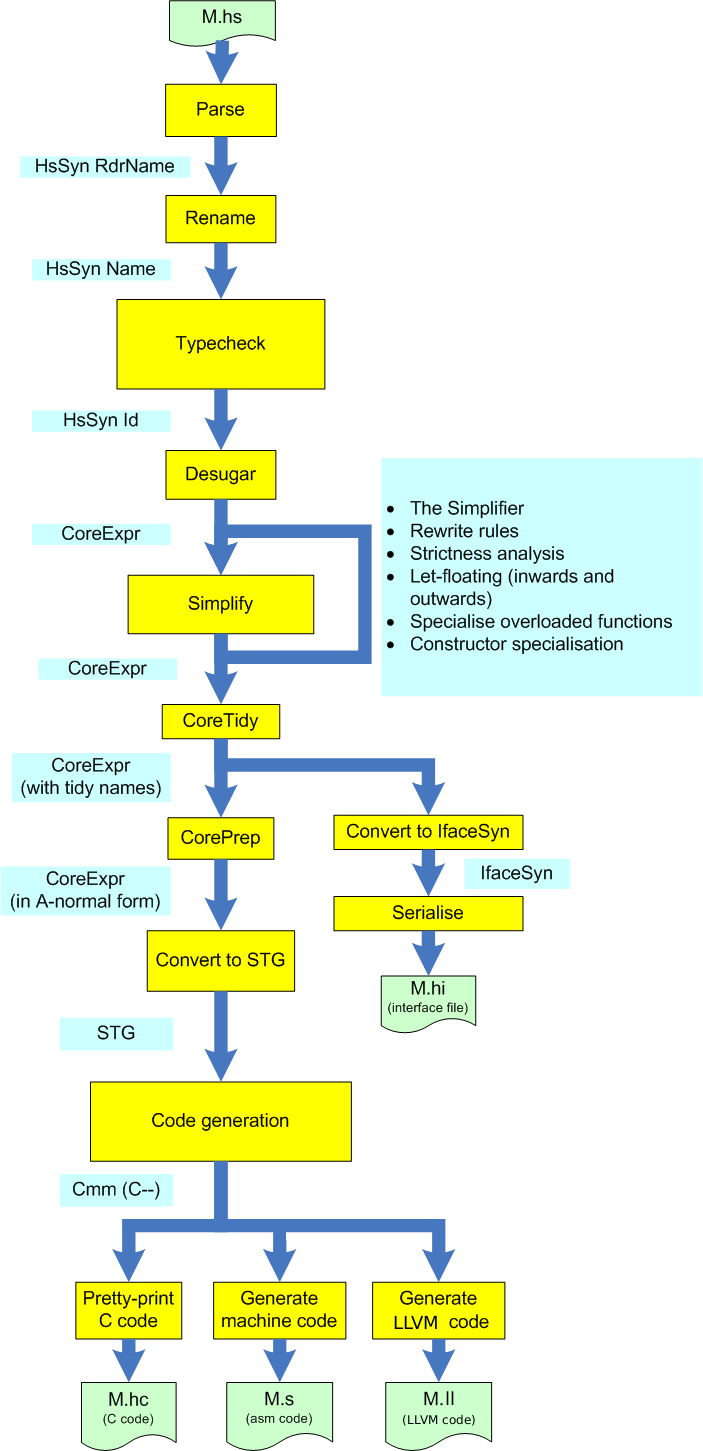
\includegraphics[scale=0.3]{HscPipe2.png}
\end{center}
\caption{The compiler phases}
\label{f:pipeline}
\end{figure}

\begin{aosasect3}{Parsing}

We start in the traditional way with parsing, which takes as input a
Haskell source file and produces as output abstract syntax.  In GHC
the abstract syntax datatype \code{HsSyn} is parameterised by the
types of the identifiers it contains, so an abstract syntax tree has
type \code{HsSyn~t} for some type of identifiers \code{t}.  This
enables us to add more information to identifiers as the program
passes through the various stages of the compiler, while reusing the
same type of abstract syntax trees.

The output of the parser is an abstract syntax tree in which the
identifiers are simple strings, which we call \code{RdrName}.  Hence,
the abstract syntax produced by the parser has type \code{HsSyn
  RdrName}.

GHC uses the tools \code{Alex} and \code{Happy} to generate its
lexical analysis and parsing code respectively, which are analogous to
the tools \code{lex} and \code{yacc} for C.

GHC's parser is purely functional.  In fact, the API of the GHC
library provides a pure function called \code{parser} that takes a
\code{String} (and a few other things) and returns either the parsed
abstract syntax or an error message.

\end{aosasect3}

\begin{aosasect3}{Renaming}

Renaming is the process of resolving all of the itentifiers in the
Haskell source code into fully-qualified names, at the same time
identifying any out-of-scope identifiers and flagging errors
appropriately.

In Haskell it is possible for a module to re-export an identifier that
it imported from another module.  For example, suppose module \code{A}
defines a function called \code{f}, and module \code{B} imports module
\code{A} and re-exports \code{f}.  Now, if a module \code{C} imports
module \code{B}, it can refer to \code{f} by the name
\code{B.f}---even though \code{f} is originally defined in module
\code{A}.  This is a useful form of namespace manipulation; it means
that a library can use whatever module structure it likes internally,
but expose a nice clean API via a few interface modules that re-export
identifiers from the internal modules.

The compiler however has to resolve all this, so that it knows what
each name in the source code corresponds to.  We make a clean
distinction between the \emph{entities}, the ``things themselves'' (in
our example, \code{A.f}), and the names by which the entities can be
referred to (e.g. \code{B.f}).  At any given point in the source code,
there are a set of entities in scope, and each may be known by one or
more different names.  The job of the renamer is to replace each of
the names in the compiler's internal representation of the code by a
reference to a particular entity.  Sometimes a name can refer to
several different entities: by itself that is not an error, but if the
name is actually used, then the renamer will flag an ambiguity error
and reject the program.

Renaming takes Haskell abstract syntax (\code{HsSyn RdrName}) as
input, and also produces abstract syntax as output (\code{HsSyn
  Name}).  Here a \code{Name} is a reference to a particular entity.

Resolving names is the main job of the renamer, but it performs a
plethora of other tasks too: collecting the equations of a function
together and flagging an error if they have differing numbers of
arguments; rearranging infix expressions according to the fixity of
the operators; spotting duplicate declarations; generating warnings
for unused identifiers, and so on.

\end{aosasect3}

\begin{aosasect3}{Typechecking}

Type checking, as one might imagine, is the process of checking that
the Haskell program is type-correct.  If the program passes the type
checker, then it is guaranteed to not crash at runtime.\footnote{The
  term ``crash'' here has a formal definition that includes hard
  crashes like ``segmentation fault'', but not things like
  pattern-matching failure.  The non-crash guarantee can be subverted
  by using certain unsafe language features, such as the Foreign
  Function Interface.}

The input to the type-checker is \code{HsSyn Name} (Haskell source
with qualified names), and the output is \code{HsSyn Id}.  An
\code{Id} is a \code{Name} with extra information: notable a
\emph{type}.  In fact, the Haskell syntax produced by the type checker
is fully decorated with type information: every identifier has its
type attached, and there is enough information to reconstruct the type
of any subexpression (which might be useful for an IDE, for example).

In practice, type checking and renaming may be interleaved, because
the Template Haskell feature generates code at runtime that itself
needs to be renamed and typechecked.

\end{aosasect3}

\begin{aosasect3}{Desugaring, and the Core language}

Haskell is a rather large language, containing many different
syntactic forms.  It is intended to be easy for humans to read and
write---there is a wide range of syntactic constructs which gives the
programmer plenty of flexibility in choosing the most appropriate
construct for the situation at hand.  However, this flexibility means
that there are often several ways to write the same code: for example,
an \code{if} expression is identical in meaning to a \code{case}
expression with \code{True} and \code{False} branches, and
list-comprehension notation can be translated into calls to
\code{map}, \code{filter}, and \code{concat}.  In fact, the definition
of the Haskell language defines all these constructs by their
translation into simpler constructs; the constructs that can be
translated away like this are called ``syntactic sugar''.

It is much simpler for the compiler if all the syntactic sugar is
removed, because the subsequent optimisation passes that need to work
with the Haskell program have a smaller language to deal with.  The
process of desugaring therefore removes all the syntactic sugar,
translating the full Haskell syntax into a much smaller language that
we call \Core{}.  We'll talk about \Core{} in detail in \aosasecref{s:core}.

\end{aosasect3}

\begin{aosasect3}{Optimisation}

Now that the program is in \Core{}, the process of optimisation
begins.  One of GHC's great strengths is in optimising away layers of
abstraction, and all of this work happens at the \Core{} level.
\Core{} is a tiny functional language, but it is a tremendously
flexible medium for expressing optimisations, ranging from the very
high level, such as strictness analysis, to the very low-level, such
as strength reduction.

Each of the optimisation passes takes \Core{} and produces
\Core{}.  The main pass here is called the \emph{Simplifier}, whose job
it is to perform a large collection of correctness-preserving
transformations on the program, with the goal of producing a more
efficient program.  Some of these transformations are simple and
obvious, such as eliminating dead code or reducing a case expression
when the value being scrutinised is known, and some are more involved,
such as function inlining and applying rewrite rules (\aosasecref{s:rules}).

The simplifier is normally run between the other optimisation passes,
of which there are about six; which passes are actually run and in
which order depends on the optimisation level selected by the user.

\end{aosasect3}

\begin{aosasect3}{Code Generation}

Once the \Core{} program has been optimised, the process of code
generation begins.  After a couple of administrative passes, the code
takes one of two routes: either it is turned into \emph{byte code} for
execution by the interactive interpreter, or it is passed to the
\emph{code generator} for eventual translation to machine code.

The code generator first converts the \Core{} into a language called
\code{STG}, which is essentially just \Core{} annotated with more
information required by the code generator.  Then, \code{STG} is translated
to \code{Cmm}, a low-level imperative language with an explicit stack. From
here, the code takes one of three routes:

\begin{aosaitemize}

\item \textbf{Native code generation}: GHC contains simple native code
  generators for a few processor architectures.  This route is fast,
  and generates reasonable code in most cases.

\item \textbf{LLVM code generation}: The \code{Cmm} is converted to
  LLVM code and passed to the LLVM compiler.  This route can produce
  significantly better code in some cases, although it takes longer
  than the native code generator.

\item \textbf{C code generation}: GHC can produce ordinary C code.
  This route produces signficantly slower code than the other two
  routes, but can be useful for porting GHC to new platforms.

\end{aosaitemize}

\end{aosasect3}

\end{aosasect2}

\end{aosasect1}

\begin{aosasect1}{Key Design Choices}

In this section we focus on a handful of the design choices that have
been particularly effective in GHC.

\begin{aosasect2}{The Intermediate Language}
\label{s:core}

\newcommand{\clift}[1]{\lfloor#1\rfloor}
\newcommand{\ol}[1]{\overline{#1}}
\newcommand{\tcase}[2]{\mathbf{case}\;#1\;\mathbf{of}\;\ol{#2}}
\newcommand{\tlet}[4]{\mathbf{let}\;#1{:}#2 = #3\;\mathbf{in}\;#4}
\newcommand{\tcast}[2]{#1\xspace\triangleright\xspace#2}
\begin{figure}
$$
\begin{array}{lrll}
\multicolumn{3}{l}{\text{Expressions}} \\
t,e,u & ::= & x  & \text{Variables} \\
      & \mid & K & \text{Data constructors} \\ 
      & \mid & k & \text{Literals} \\
      & \mid & \lambda x{:}\sigma \code{.} e \mid e\;u 
             & \text{Value abstraction and application} \\ 
    & \mid   &  \Lambda a{:}\eta \code{.} e \mid e\;\phi
             & \text{Type abstraction and application} \\ 
    & \mid    & \mathbf{let}\;\ol{x:\tau = e}\;\mathbf{in}\;u 
             & \text{Local bindings} \\ 
    & \mid    & \tcase{e}{p \to u} 
             & \text{Case expressions} \\ 
    & \mid    & \tcast{e}{\gamma}         &  \text{Casts} \\
    & \mid    & \clift{\gamma}            &  \text{Coercions} \\[2mm] 
 p  & ::=     & K\; \ol{c{:}\eta}\;\;\ol{x{:}\tau} & \text{Patterns} \\[3mm]
\end{array} 
$$
\label{fig:core-syntax}
\caption{The syntax of \Core{}}
\end{figure}

A typical structure for a compiler for a statically-typed language is
this: the program is typechecked, and transformed to some
\emph{untyped} intermediate language, before being optimised.  GHC is
different: it has a \emph{statically-typed intermediate language}.  As
it turns out, this design choice has had a pervasive effect on the
design and development of GHC.

GHC's intermediate language is called \Core{} (when thinking of the
implementation) or System FC (when thinking about the theory).  Its
syntax is given in \aosafigref{fig:core-syntax}.  The exact details
are not imortant here; the intersted reader can consult
\citet{bib:system-f} for more details.  For our present purposes,
however, the following points are the key ones:

\begin{aosaitemize}

\item Haskell is a very large source language.  The data type
  representing its syntax tree has literally hundreds of constructors.

  In contrast \Core{} is a tiny, principled, lambda calculus.  It has
  extremely few syntactic forms, yet we can translate all of Haskell
  into \Core{}.

\item Haskell is an \emph{implicitly-typed} source language.  A
  program may have few or no type annotations; instead it is up to the
  type inference algorithm to figure out the type of every binder and
  sub-expressions.  This type inference algorithm is complex, and
  occasionally somewhat \emph{ad-hoc}, reflecting the design
  compromises that every real programming language embodies.

  In contrast \Core{} is an \emph{explicitly-typed} language.  Every
  binder has an explicit type, and terms include explicit type
  abstractions and applications.  \Core{} enjos a very simple, fast
  type checking algorithm, that checks that the program is type
  correct.  The algorithm is entirely straightforward; there are no
  \emph{ad-hoc} compromises.

\end{aosaitemize}

All of GHC's analysis and optimisation passes work on \Core{}. This is
great: because \Core{} is such a tiny language an optimisation has
only a few cases to deal with.  Although \Core{} is small, it is
extremely expressive---System F was, after all, originally developed
as a foundational calculus for typed computation.  When new language
features are added to the source language (and that happens all the
time!) the changes are usually restricted to the front end; \Core{}
stays unchanged, and hence so does most of the compiler.

But why is \Core{} typed?  After all, if the type inference engine
accepts the source program, that program is presumably well typed, and
each optimisation pass presumably maintains that type-correctness.
\Core{} may enjoy a fast type checking algorithm, but why would you
ever want to run it?  Moreover, making \Core{} typed carries
significant costs, because every transformation or optimisation pass
must produce a well-typed program, and generating all those type
annotations is often non-trivial.

Nevertheless, it has been huge win to have an explicitly-typed
intermediate language, for several reasons:

\begin{aosaitemize}

\item Running the \Core{} type checker (we call it \Lint{}) is a very
  powerful consistency check on the compiler itself.  Imagine that you
  write an ``optimisation'' that accidentally generates code that
  treats an integer value as a function, and tries to call it.  The
  chances are that the program will segmentation fault, or fail at
  runtime in a bizarre way. Tracing a seg-fault back to the particular
  optimisation pass that broke the program is a long road.

  Now imagine instead that we run \Lint{} after every optimisation
  pass (and we do, if you use the flag \code{-dcore-lint}): it will
  report a precisely-located error immediately after the offending
  optimsiation.  What a blessing.

  Of course, type soundness is not the same as correctness: \Lint{}
  will not signal an error if you ``optimise'' $(x*1)$ to $1$ instead
  of to $x$.  But if the program passes \Lint{}, it will guarantee to
  run without seg-faults; and moreover in practice we have found that
  it is surprisingly hard to accidentally write optimisations that are
  type-correct but not semantically correct!

  \item The type inference algorithm for Haskell is very large and
    very complex: a glance at \aosafigref{f:lines} confirms that the
    type checker is by far the largest single component of GHC.  Large
    and complex means error-prone.  But \Lint{} serves as an 100\%
    independent check on the type inference engine: if the type
    inference engine accepts a program that is not, in fact,
    type-corect, \Lint{} will reject it. So \Lint{} serves as a
    powerful auditor of the type inference engine.

\item The existence of \Core{} has also proved to be a tremendous
  sanity check on the \emph{design} of the source language.  Our users
  constantly suggest new features that they would like in the
  language. Sometimes these features are manifestly ``syntactic
  sugar'', convenient new syntax for something you can do already. But
  sometimes they are deeper, and it can be hard to tell how
  far-reaching the feature is.

  \Core{} gives us a precise way to evaluate such features.  If the
  feature can readily be translated into \Core{}, that reassures us
  that nothing fundamentally new is going on: the new feature is
  syntactic-sugar-like. On the other hand, if it would require an
  extension to \Core, then we think much, much more carefully.

\end{aosaitemize}

In practice \Core{} has been incredibly stable: over a 20-year time
period we have added exactly one new major feature to \Core{} (namely
coercions and their associated casts).  Over the same period, the
source languaage has evolved enormously.  We attribte this stability
not to our own brilliance, but rather to the fact that \Core{} is
based dirctly on foundational mathematics: bravo Girard!

\end{aosasect2}

\begin{aosasect2}{Typechecking the Source Language}

One interesting design decision is whether type-checking should be
done before or after desugaring.  The trade-offs are these:

\begin{aosaitemize}

\item Typechecking before desugaring means that the type checker must
  deal directly with Haskell's very large syntax, so the typechecker
  has many cases to consider.  If we desugared into (an untyped
  variant of) \Core{} first, one might hope that the type checker
  would become much smaller.

\item On the other hand, typechecking after desugaring would impose a
  significant new obligation: that desugaring does not affect which
  programs are type-correct.  After all, desugaring implies a
  deliberate loss of information.  It is probably the case that in
  95\% of the cases there no problem, but \emph{any} problem here
  would force some compromise in the design of \Core{} to preserve
  some extra information.

\item Most seriously of all, typechecking a desugared program would
  make it much harder to report errors that relate to the original
  program text, and not to its (sometimes elaborate) desugared
  version.

\end{aosaitemize}

Most compilers typecheck after desugaring, but for GHC made the
opposite choice: we typecheck the full original Haskell syntax, and
then desugar the result.  It sounds as if adding a new syntactic
construct might be complicated, but (following the French school) we
have structured the type inference engine in a way that makes it
easy. Type inference is split into two parts:

\begin{aosaenumerate}

\item Constraint generation: walk over the source syntax tree,
  generating a collection of type constraints.  This step deals with
  the full syntax of Haskell, but it is very straightforward code, and
  it is easy to add new cases.

\item Constraint solving: solve the gathered constraints.  This is
  where the subtlety of the type inference engine lies, but it is
  independent of the source language syntax, and would be the same for
  a much smaller or much larger language.

\end{aosaenumerate}

On the whole, the typecheck-before-desugar design choice has turned
out to be a big win.  Yes, it adds lines of code to the typechecker,
but they are \emph{simple} lines. It avoids giving two conflicting
roles to the same data type, and makes the type inference engine less
complex, and easier to modify. Moreover, GHC's type error messages are
pretty good.

\end{aosasect2}

\begin{aosasect2}{No Symbol Table}

Compilers usually have one or more data structures known as
\emph{symbol tables}, which are mappings from symbols
(e.g.\ variables) to some information about the variable, such as its
type, or where in the source code it was defined.

In GHC we use symbol tables quite sparingly; mainly in the renamer and
type checker.  As far as possible, we use an alternative strategy: a
variable is a data structure that \emph{contains} all the information
about itself.  Indeed, a large amount of information is reachable by
traversing the data structure of a variable: from a variable we can
see its type, which contains type constructors, which contain their
data constructors, which themselves contain types, and so on.  For
example, here are some data types from GHC (heavily abbreviated and
simplified):

\begin{verbatim}
  data Id      = MkId Name Type
  data Type    = TyConApp TyCon [Type]
               | ....
  data TyCon   = AlgTyCon Name [DataCon]
               | ...
  data DataCon = MkDataCon Name Type ...
\end{verbatim}

An \code{Id} contains its \code{Type}.  A \code{Type} might be an
application of a type constructor to some arguments (e.g. \code{Maybe
  Int}), in which case it contains the \code{TyCon}.  A \code{TyCon}
can be an algebraic data type, in which case it includes a lits of its
data constructors.  Each \code{DataCon} includes its \code{Type},
which of course mentions the \code{TyCon}.  And so on.  The whole
structure is highly interconnected.  Indeed it is cyclic; for example,
a \code{TyCon} may contain a \code{DataCon} which contains a
\code{Type}, which contains the very \code{TyCon} we started with.

This approach has some advantages and disadvantages:

\begin{aosaitemize}

\item Many queries that would require a lookup in a symbol table are
  reduced to a simple field access, which is great for efficiency and
  code clarity.

\item There is no need to carry around extra symbol tables, the
  abstract syntax tree already contains all the information.

\item The space overheads are better: all instances of the same
  variable share the same data structure, and there is no space needed
  for the table.

\item The only difficulties arise when we need to \emph{change} any of
  the information associated with a variable.  This is where a symbol
  table has the advantage: we would just change the entry in the
  symbol table.  In GHC we have to traverse the abstract syntax tree
  and replace all the instances of the old variable with the new one;
  indeed the simplifier does this regularly, as it needs to update
  certain optimisation-related information about each variable.

\end{aosaitemize}

It is hard to know whether it would be better or worse overall to use
symbol tables, because this aspect of the design is so fundamental
that it is almost impossible to change.  Still, avoiding symbol tables
is a natural choice in the purely functional setting, so it seems
likely that this approach is a good choice for Haskell.

\end{aosasect2}

\begin{aosasect2}{Inter-Module Optimisation}

Functional languages encourage the programmer to write small
definitions.  For example, here is the definition of \code{&&} from
the standard library:

\begin{verbatim}
(&&) :: Bool -> Bool -> Bool
True && True = True
_    && _    = False
\end{verbatim}

If every use of such a function really required a function call,
efficency would be terrible.  One solution is to make the compiler
treat certain functions specially; another is to use a pre-processor
to replace a ``call'' with the desired inline code.  All of these
solutions are unsatisfactory in one way or another, especially as
another solution is so obvious: simply inline the function.  To
``inline a function'' means to replace the call by a copy of the
function body, suitably instantiating its parameters.

In GHC we have systematically adopted this approach \cite{bib:inlining}.
Virtually nothing is built into the compiler.  Instead, we define as
much as possible in libraries, and use aggressive inlining to elimiate
the overheads.  This means that \emph{programmers can define their own
  libraries that will be inlined and optimised as well as the ones tha
  come with GHC}.

A consequence is that GHC must be able to do cross-module, and indeed
cross-package, inlining.  The idea is simple:

\begin{aosaitemize}

\item When compiling a Haskell module \code{Lib.hs}, GHC produces
  object code in \code{Lib.o} and an ``interface file'' in
  \code{Lib.hi}.  This interface file contains information about all
  the functions that \code{Lib} exports, including both their types
  and, for sufficiently small functions, their definitions.

\item When compiling a module \code{Client.hs} that imports
  \code{Lib}, GHC reads the interface \code{Lib.hi}.  So if
  \code{Client} calls a function \code{Lib.f} defined in \code{Lib},
  GHC can use the information in \code{Lib.hi} to inline \code{Lib.f}.

\end{aosaitemize}

By default GHC will expose the definition of a function in the
interface file only if the function is ``small'' (there are flags to
control this size threshold).  But we also support an INLINE pragma,
to instruct GHC to inline the definition agreessively at call sites,
regardless of size, thus:

\begin{verbatim}
foo :: Int -> Int 
{-# INLINE foo #-}
foo x = <some big expression>
\end{verbatim}

Cross-module inlining is absolutely essential for defining
super-efficient libraries, but it does come with a cost.  If the
author upgrades his library, it is not enough to re-link
\code{Client.o} with the new \code{Lib.o}, because \code{Client.o}
contains inlined fragments of the old \code{Lib.hs}, and they may well
not be compatible with the new one.  Another way to say this is that
the ABI (Application Binary Interface) of \code{Lib.o} has changed in
a way that requires recompilation of its clients.

In fact, the only way for compilation to generate code with a fixed,
predictable, ABI is to disable cross-module optimisation, and this is
typically too high a price to pay for ABI compatibility.  Users
working with GHC will usually have the source code to their entire
stack available, so recompiling is not normally an issue (and, as we
will describe later, the package system is designed around this mode
of working).  However, there are situations where recompiling is not
practical: distributing bug fixes to libraries in a binary OS
distribution, for example.  In the future we hope it may be possible
to find a compromise solution that allows retaining ABI compatibility
while still allowing some cross-module optimisation to take place.

\end{aosasect2}

\end{aosasect1}

\begin{aosasect1}{Extensibility}

It is often the case that a project lives or dies according to how
extensible it is.  A monolithic piece of software that is not
extensible has to do everything and do it right, whereas an extensible
piece of software can be a useful base even if it doesn't provide all
the required functionality out of the box.

Open source projects are of course extensible by definition, in that
anyone can take the code and add their own features.  But modifying
the original source code of a project maintained by someone else is
not only a high-overhead approach, it is also not conducive to sharing
your extension with others.  Therefore successful projects tend to
offer forms of extensibility that do not involve modifying the core
code, and GHC is no exception in this respect.

\begin{aosasect2}{User-Defined Rewrite Rules}
\label{s:rules}

The core of GHC is a long sequence of optimisation passes, each of
which performs some semantics-preserving transformormation, \Core{}
into \Core{}.  But the author of a library defines functions that
often have some non-trivial, domain-specific transformations of their
own, ones that cannot possibly be predicted by GHC. So GHC allows
library authors to define \emph{rewrite rules} that are used to
rewrite the program during optimisation
\cite{bib:playing-by-the-rules}.  In this way, programmers can,
in effect, extend GHC with domain-specific optimisations.

One example is the \code{foldr/build} rule, which is expressed like this:
\begin{verbatim}
{-# RULES "fold/build"    
    forall k z (g::forall b. (a->b->b) -> b -> b) . 
       foldr k z (build g) = g k z
 #-}
\end{verbatim}

The entire rule is a pragma, introduce by \code{{-# RULES}.  The rule
  says that whenever GHC sees the expression \code{(foldr k z (build
    g))} it should rewrite it to \code{(g k z)}.  This transformation
  is semantics-preserving, but it takes a research paper to argue that
  it is \cite{bib:gill-short-cut}, so there is no chance of GHC performing
  it automatically.  Together with a handful of other rules, and some
  INLINE pragmas, GHC is able to fuse together list-transforming
  functions.  For example, the two loops in \code{(map f (map g xs))}
  are fused into one.

Although rewrite rules are simple and easy to use, they have proved to
be a very powerful extension mechanism.  When we first introduced the
feature into GHC, ten years ago, we expected it to be an
occasionally-useful facility.  But in practice it has turned out to be
useful in very many libraries, whose efficiency often depends
crucially on rewrite rules.  For example, GHC's own \code{base}
library contains upward of 100 rules, while the popular \code{vector}
library uses several dozen.

\end{aosasect2}

\begin{aosasect2}{Compiler Plugins}

One way in which a compiler can offer extensibility is to allow
programmers to write a pass that is inserted dirctly into the
compiler's pipeline.  Such passes are often called ``plugins''.  GHC
supports plugins in the following way:

\begin{aosaitemize}

\item The programmer writes a \Core{} to \Core{} pass, as an ordinary
  Haskell function in a module \code{P.hs}, say, and compiles it to
  object code.

\item When compiling some module, the programmer uses the command-line
  flag \code{-plugin P}.  (Alternatively, he can give the flag in a
  pragma at the start of the module.)

\item GHC searches for \code{P.o}, dynamically links it into the
  running GHC binary, and calls it at the appropriate point in the
  pipeline

\end{aosaitemize}

But what is ``the appropriate point in the pipeline''?  GHC does not
know, and so it allow the plugin to make that decision.  As a result
of this and other matters, the API that the plugin must offer is a bit
more complicated than a single \Core{} to \Core{} function---but not
much.

Plugins sometimes require, or produce, auxiliary plugin-specific data.
For example, a plugin might perform some analysis on the functions in
the module being compiled (\code{M.hs}, say), and might want to put
that information in the interface file \code{M.hi}, so that the plugin
has access to that information when compiling modules that import
\code{M}.  GHC offers an annotation mechanism to support this.

Plugins and annotations are relatively new to GHC.  They have a higher
barrier to entry than rewrite rules, because the plugin is
manipulating GHC's internal data structures, but of course they can do
much more.  It remains to be seen how widely they will be used.

\end{aosasect2}

\begin{aosasect2}{GHC as a Library: the GHC API}
\label{s:ghcapi}

One of GHC's original goals was to be a \emph{modular} foundation that
others could build on.  We wanted the code of GHC to be as transparent
and well-documented as possible, so that it could be used as the basis
for research projects by others; we imagined that people would want to
make their own modifications to GHC to add new experimental features
or optimisations.  Indeed, there have been some examples of this: for
example, there exists a version of GHC with a Lisp front-end, and a
version of GHC that generates Java code, both developed entirely
separately by individuals with little or no contact with the GHC team.

However, producing modified versions of GHC represents only a small
subset of the ways in which the code of GHC can be re-used.  As the
popularity of the Haskell language has grown, there has been an
increasing need for tools and infrastructure that understand Haskell
source code, and GHC of course contains a lot of the functionality
necessary for building these tools: a Haskell parser, abstract syntax,
type checker and so on.

With this in mind, we made a simple change to GHC: rather than
building GHC as a monolithic program, we build GHC as a
\emph{library}, that is then linked with a small \emph{Main} module to
make the GHC executable itself, but also shipped in library form so
that users can call it from their own programs.  At the same time we
built an API to expose GHC's funcionality to clients.  The API
provides enough functionality to implement the GHC batch compiler and
the GHCi interactive environment, but it also provides access to
individual passes such as the parser and type checker, and allows the
data structures produced by these passes to be inspected.  This change
has given rise to a wide range of tools built using the GHC API,
including:

\begin{aosaitemize}

\item A documentation tool,
  \emph{Haddock}\footnote{\url{http://www.haskell.org/haddock/}},
  which reads Haskell source code and produces HTML documentation

\item New versions of the GHCi front end with additional features,
  e.g. \emph{ghci-haskeline}\footnote{\url{http://hackage.haskell.org/package/ghci-haskeline}}
  which was subsequently merged back into GHC,

\item IDEs that offer advanced navigation of Haskell source code,
  e.g. \emph{Leksah}\footnote{\url{http://hackage.haskell.org/package/leksah}},

\item
  \emph{hint}\footnote{\url{http://hackage.haskell.org/package/hint}},
  a simpler API for on-the-fly evaluation of Haskell source code.

\end{aosaitemize}

\end{aosasect2}

\begin{aosasect2}{The Package System}

The package system has been a key factor in the growth in use of the
Haskell language in recent years.  Its main purpose is to enable
Haskell programmers to share code with each other, and as such is an
important aspect of extensibility: the package system extends the
shared codebase beyond GHC itself.

The package system embodies various pieces of infrastructure that
together make sharing code easy.  With the package system as the
enabler, the community has built a large body of shared code; rather
than relying on libraries from a single source, Haskell programmers
draw on libraries developed by the whole community.  This model has
worked well for other languages: CPAN for Perl for example, although
Haskell being a predominantly compiled rather than interpreted
language presents a somewhat different set of challanges.

Basically, the package system lets a user manage libraries of Haskell
code written by other people, and use them in their own programs and
libraries.  Installing a Haskell library is as simple as uttering a
single command, e.g.

\begin{verbatim}
$ cabal install zlib
\end{verbatim}

\noindent
downloads the code for the \code{zlib} package from
\url{http://hackage.haskell.org}, compiles it using GHC, installs the
compiled code somewhere on your system (e.g.\ in your home directory
on a Unix system), and registers the installation with GHC.
Furthermore, if \code{zlib} depends on any other packages that are not
yet installed, those will also be downloaded, compiled and installed
automatically before \code{zlib} itself is compiled.  It is a
tremendously smooth way to work with libraries of Haskell code shared
by others.

The package system is made of four components, only the first of which
is strictly part of the GHC project:

\begin{aosaitemize}

\item Tools for managing the \emph{package database}, which is simply
  a repository for information about the packages installed on your
  system.  GHC reads the package database when it starts up, so that
  it knows which packages are available and where to find them.

\item A library called \code{Cabal} (Common Architecture for Building
  Applications and Libraries), which implements functionality for
  building, installing and registering individual packages.

\item A website at \url{http://hackage.haskell.org} which hosts
  packages written and uploaded by users.  The website automatically
  builds documentation for the packages which can be browsed online.
  At the time of writing, Hackage is hosting over 3000 packages
  covering functionality including database libraries, web frameworks,
  GUI toolkits, data structures, and networking.

\item The \code{cabal} tool which ties together the Hackage website
  and the \code{Cabal} library: it downloads packages from Hackage,
  resolves dependencies, and builds and installs packages in the right
  order.  New packages can also be uploaded to Hackage using
  \code{cabal} from the command line.

\end{aosaitemize}

These components have been developed over several years by members of
the Haskell community and the GHC team, and together they make a
system that fits perfectly with the Open Source development model.
There are no barriers to sharing code or using code that others have
shared (provided you respect the relevant licenses, of course).  You
can be using a package that someone else has written literally within
seconds of finding it on Hackage.

Hackage has been so successful that the remaining problems it has are
now those of scale: users find it difficult to choose amongst the four
different database frameworks, for example.  Ongoing developments are
aimed at solving these problems in ways that leverage the community.
For example, allowing users to comment and vote on packages will make
it easier to find the best and most popular packages, and collecting
data on build success or failures from users and reporting the results
will help users avoid packages that are unmaintained or have problems.

\end{aosasect2}

\end{aosasect1}

\begin{aosasect1}{The Runtime System}
\label{s:rts}

The Runtime System (hereafter, the RTS) is a library of mostly C code
that is linked into every Haskell program.  It provides the support
infrastructure needed for running the compiled Haskell code, including
the following main components:

\begin{aosaitemize}

\item Memory management, including a parallel, generational, garbage
  collector;

\item Thread management and scheduling;

\item The primitive operations provided by GHC;

\item A bytecode interpreter and dynamic linker for GHCi.

\end{aosaitemize}

The rest of this section is divided into two: first we focus on a
couple of the aspects of the design of the RTS that we consider to
have been successful and instrumental in making it work so well, and
secondly we talk about the coding practices and infrastructure we have
built in the RTS for coping with what is a rather hostile programming
environment.

\begin{aosasect2}{Key Design Decisions}

In this section we describe two of the design decisions in the RTS
that we consider to have been particularly successful.

\begin{aosasect3}{The Block Layer}

The garbage collector is built on top of a \emph{block layer} that
manages memory in units of blocks, where a block is a multiple of 4KB
in size.  The block layer has a very simple API:

\begin{verbatim}
typedef struct bdescr_ {
    void *               start;
    struct bdescr_ *     link;
    struct generation_ * gen;   // generation
    // .. various other fields
} bdescr;

bdescr * allocGroup (int n);
void     freeGroup  (bdescr *p);
bdescr * Bdescr     (void *p);  // a macro
\end{verbatim}

This is the only API used by the garbage collector for allocating and
deallocating memory.  Blocks of memory are allocated with
\code{allocGroup} and freed with \code{freeGroup}.  Every block has a
small structure associated with it called a \emph{block descriptor}
(\code{bdescr}).  The operation \code{Bdescr(p)} returns the block
descriptor associated with an arbitrary address \code{p}; this is
purely an address calculation based on the value of \code{p} and
compiles to a handful of arithmetic and bit-manipulation instructions.

Blocks may be linked together into chains using the \code{link} field
of the \code{bdescr}, and this is the real power of the technique.
The garbage collector needs to manage several distinct areas of memory
such as \emph{generations}, and each of these areas may need to grow
or shrink over time.  By representing memory areas as linked lists of
blocks, the GC is freed from the difficulties of fitting multiple
resizable memory areas into a flat address space.

The implementation of the block layer uses techniques that are
well-known from C's \code{malloc()/free()} API: it maintains lists of
free blocks of various sizes, and coalesces free areas.  The
operations \code{freeGroup()} and \code{allocGroup()} are carefully
designed to be O(1).

One major advantage of this design is that it needs very little
support from the OS, and hence is great for portability.  The block
layer needs to allocate memory in units of 1MB, aligned to a 1MB
boundary.  While none of the common OSs provide this functionality
directly, it is implementable without much difficulty in terms of the
facilities they do provide.  The payoff is that GHC has no dependence
on the particular details of the addresss-space layout used by the OS,
and it coexists peacefully with other users of the address space, such
as shared libraries and operating system threads.

There is a small up-front complexity cost for the block layer, in
terms of managing chains of blocks rather than contiguous memory.
However, we have found that this is a cost is more than repaid in
flexibility and portabilty; for example, the block layer enabled a
particularly simple algorithm for parallel GC to be implemented
\cite{bib:parallel-gc}.

\end{aosasect3}

\begin{aosasect3}{Lightweight Threads and Parallelism}

We consider concurrency to be a vitally important programming
abstraction, particularly for building applications like web servers
that need to interact with large numbers of external agents
simultaneously.  If concurrency is an important abstraction, then it
should not be so expensive that programmers are forced to avoid it, or
build elaborate infrastructure to amortise its cost (e.g.\ thread
pools).  We believe that concurrency should just work, and be cheap
enough that you don't worry about forking threads for small tasks.

All operating systems provide threads that work perfectly well, the
problem is that they are far too expensive.  Typical OSs struggle to
handle thousands of threads, whereas we want to manage threads by the
million.

Green threads, otherwise known as ligthweight threads or user-space
threads, are a well-known technique for avoiding the overhead of
operating system threads.  The idea is that threads are managed by the
program itself, or a library (in our case, the RTS), rather than by
the operating system.  Managing threads in user space should be
cheaper, because fewer traps into the operating system are required.

In the GHC RTS we take full advantage of this idea.  A context switch
only occurs when the thread is at a \emph{safe point}, where very
little additional state needs to be saved.  Because we use accurate
GC, the stack of the thread can be moved and expanded or shrunk on
demand.  Contrast these with OS threads, where every context switch
must save the entire processor state, and where stacks are immovable
so a large chunk of address space has to be reserved up front for each
thread.

Green threads can be vastly more efficient than OS threads, so why
would anyone want to use OS threads?  It comes down to three main
problems:

\begin{aosaitemize}

\item Blocking and foreign calls.  A thread should be able to make a
  call to an OS API or a foreign library that blocks, without blocking
  all the other threads in the system.

\item Parallelism.  Threads should automatically run in parallel if
  there are multiple processor cores on the system.

\item Some external libraries (notably OpenGL and some GUI libraries)
  have APIs that must be called from the same OS thread each time,
  because they use thread-local state.

\end{aosaitemize}

It turns out that all of these are difficult to arrange with green
threads.  Nevertheless, we persevered with green threads in GHC and
found solutions to all three:

\begin{aosaitemize}

\item When a Haskell thread makes a foreign call, another OS thread
  takes over the execution of the remaining Haskell threads
  \cite{bib:concffi04}.  A small pool of OS threads are maintained for
  this purpose, and new ones are created on demand.

\item GHC's scheduler multiplexes many lightweight Haskell threads
  onto a few heavyweight OS threads; it implements a transparent M:N
  threading model.  Typically N is chosen to be the same as the number
  of processor cores in the machine, allowing real parallelism to take
  place but without the overhead of having a full OS thread for each
  lightweight Haskell thread.

  In order to run Haskell code, an OS thread must hold a
  \emph{Capability}\footnote{we have also called it a ``Haskell
    Execution Context'', but the code currently uses the Capability
    terminology}: a data structure that holds the resources required
  to execute Haskell code, such as the nursery (memory where new
  objects are created).  Only one OS thread may hold a given
  Capability at a time.

\item We provide an API for creating a \emph{bound thread}: a Haskell
  thread that is tied to one specific OS thread, such that any foreign
  calls made by this Haskell thread are guaranteed to be made by that
  OS thread.

\end{aosaitemize}

So in the vast majority of cases, Haskell's threads behave exactly
like OS threads: they can make blocking OS calls without affecting
other threads, and they run in parallel on a multicore machine.  But
they are orders of magnitude more efficient, in terms of both time and
space.

Having said that, the implementation does have one problem that users
occasionally run into, especially when running benchmarks.  We
mentioned above that lightweight threads derive some of their
efficiency by only context-switching at ``safe points'', points in the
code that the compiler designates as safe, where the internal state of
the virtual machine (stack, heap, registers etc.) is in a tidy state
and garbage collection could take place.  In GHC, a safe point is
whenever memory is allocated; which in almost all Haskell programs
happens regularly enough that the program never executes more than a
few tens of instructions without hitting a safe point.  However, it is
possible in highly optimised code to find loops that run for many
iterations without allocating memory.  This tends to happen often in
benchmarks (e.g.\ functions like factorial and fibonacci).  It occurs
less often in real code, although it does happen.  The lack of safe
points prevents the scheduler from running, which can have detrimental
effects.  It is possible to solve this problem, but not without
impacting the performance of these loops, and often people care about
saving every cycle in their inner loops.  This may just be a
compromise we have to live with.

\end{aosasect3}

\end{aosasect2}

\end{aosasect1}

\begin{aosasect1}{Developing GHC}

GHC is a single project with a twenty-year life span, and is still in
a ferment of innovation and development.  For the most part our
infrastructure and tooling has been conventional.  For example, we use
a bug tracker (Trac), a wiki (also Trac), and use Git for revision
control. (This revision-control mechanism evolved from purely manual,
then CVS, then Darcs, before finally moving to Git in 2010.)  There
are a few points that may be less universal, and we offer them here.

\begin{aosasect2}{Comments and Notes}

One of the most serious difficulties in a large, long-lived project is
keeping technical documetation up to date.  We have no silver bullet,
but we offer one low-tech mechanism that has served us particularly
well: \code{Notes}.

When writing code, there is often a moment when a careful programmer
will mentally say something like ``This data type has an important
invariant''.  She is faced with two choices, both unsatisfactory.  She
can add the invariant as a comment, but that can make the data type
declaration too long, so that it is hard to see what the constructors
are.  Alternatively , she can document the invariant elsewhere, and
risk it going out of date.  Over twenty years, \emph{everything} goes
out of date!

Thus motivated, we developed the following very simple convention:

\begin{aosaitemize}

\item Comments of any significant size are not interleaved with code,
  but instead set off by themselves, with a heading in standard form,
  thus:

\begin{verbatim}
  Note [Equality-constrained types]
  ~~~~~~~~~~~~~~~~~~~~~~~~~~~~~~~~~
  The type   forall ab. (a ~ [b]) => blah
  is encoded like this:

     ForAllTy (a:*) $ ForAllTy (b:*) $
     FunTy (TyConApp (~) [a, [b]]) $
     blah
\end{verbatim}

\item A the point where the comment is relevant, we add a short
  comment referring to the Note:

\begin{verbatim}
 data Type
   = FunTy Type Type
	-- See Note [Equality-constrained types]

   | ...
\end{verbatim}

  The comment highlights that something interesting is going on, and
  gives a precise reference to the comment that explains.  It sounds
  trivial, but the precision is vastly better than our previous habit
  of saying ``see the comment above'', because it often was not clear
  \emph{which} of the many comments above was intended, and after a
  few years the comment was not even above (it was below; or gone
  altogether).

\end{aosaitemize}

Not only is it possible to go from the code that refers to the
\code{Note} to the \code{Note} itself, but the reverse is also
possible, and that is often useful.  Moreover, the same \code{Note}
may be referred to from multiple points in the code.

This simple, ASCII-only technique, with no automated support, has
transformed our lives: GHC has around 800 \code{Notes}, and the number
grows daily.

\end{aosasect2}

\begin{aosasect2}{How to Keep On Refactoring}

The code of GHC is churning just as quickly, if not more so, than it
was ten years ago.  There is no doubt that the complexity of the
system has increased manyfold over that same time period: we saw
measures of the amount of code in GHC earlier.  Yet, the system
remains manageable.  We attribute this to three main factors:

\begin{aosaitemize}

\item There's no substitute for good software engineering.  Modularity
  always pays off: making the APIs between components as small as
  possible makes the individual components more flexible because they
  have fewer interdependencies.  For example, GHC's \Core datatype
  being small reduces the coupling between Core-to-Core passes, to the
  extent that they are almost completely independent and can be run in
  an arbitrary order.

\item Developing in a strongly-typed language makes refactoring a
  breeze.  Whenever we need to change a data type, or change the
  number of arguments or type of a function, the compiler immediately
  tells us what other places in the code need to be fixed.  Simply
  having an absolute guarantee that a large class of errors have been
  statically ruled out saves a huge amount of time, especially when
  refactoring.  It is scary to imagine how many hand-written test
  cases we would need to provide the same level of coverage that the
  type system provides.

\item When programming in a purely functional language, it is hard to
  introduce accidental dependencies via state.  If you decide that you
  suddenly need access to a piece of state deep in an algorithm, in an
  imperative language you might be tempted to just make the state
  globally visible rather than explicitly pass it down to the place
  that needs it.  This way eventually leads to a tangle of invisible
  dependencies, and \emph{brittle code}: code that breaks easily when
  modified.  Pure functional programming forces you to make all the
  dependencies explicit, which exerts some negative pressure on adding
  new dependencies, and fewer dependencies means greater modularity.
  Certainly when it is \emph{necessary} to add a new dependency then
  purity makes you write more code to express the dependency, but in
  our view it is a worthwhile price to pay for the long-term health of
  the code base.

  As an added benefit, purely functional code is thread-safe by
  construction and tends to be easier to parallelise.

\end{aosaitemize}

\end{aosasect2}

\begin{aosasect2}{Crime Doesn't Pay}

Looking back over the changes we've had to make to GHC as it has
grown, a common lesson emerges: being less than purely functional,
whether for the purposes of efficiency or convenience, tends to have
negative consequences down the road.  We have a couple of great
examples of this:

\begin{aosaitemize}

\item GHC uses a few data structures that rely on mutation internally.
  One is the \code{FastString} type, which uses a single global hash
  table; another is a global \code{NameCache} that ensures all
  external names are assigned a unique number.  When we tried to
  parallelise GHC (that is, make GHC compile multiple modules in
  parallel on a multicore processor), these data structures based on
  mutation were the \emph{only} sticking points.  Had we not resorted
  to mutation in these places, GHC would have been almost trivial to
  parallelise.

  In fact, although we did build a prototype parallel version of GHC,
  GHC does not currently contain support for parallel compilation, but
  that is largely because we have not yet invested the effort required
  to make these mutable data structures thread-safe.

\item GHC's behaviour is governed to a large extent by command-line
  flags.  These command-line flags are by definition constant over a
  given run of GHC, so in early versions of GHC we made the values of
  these flags available as top-level constants. For example, there was
  a top-level value \code{opt\_GlasgowExts} of type \code{Bool}, that
  governed whether certain language extensions should be enabled or
  not.  Top-level constants are highly convenient, because their
  values don't have to be explicitly passed as arguments to all the
  code that needs access to them.

  Of course these options are not really \emph{constants}, because
  they change from run to run, and the definition of
  \code{opt\_GlasgowExts} involves calling \code{unsafePerformIO}
  because it hides a side effect.  Nevertheless, this trick is
  normally considered ``safe enough'' because the value is constant
  within any given run; it doesn't invalidate compiler optimisations,
  for example.

  However, GHC was later extended from a single-module compiler to a
  multi-module compiler.  At this point the trick of using top-level
  constants for flags broke, because the flags may have different
  values when compiling different modules.  So we had to refactor
  large amounts of code to pass around the flags explicitly.

  Perhaps you might argue that treating the flags as \emph{state} in
  the first place, as would be natural in an imperative language,
  would have sidestepped the problem.  To some extent this is true,
  although purely functional code has a number of other behefits, not
  least of which is that representing the flags by an immutable data
  structure means that the resulting code is already thread-safe and
  will run in parallel without modification.

\end{aosaitemize}

\end{aosasect2}

\begin{aosasect2}{Developing the RTS}

GHC's runtime system presents a stark contrast to the compiler in many
ways.  There is the obvious difference that the runtime system is
written in C rather than Haskell, but there are also considerations
unique to the RTS that give rise to a different design philosophy:

\begin{aosaenumerate}

\item Every Haskell program spends a lot of time executing code in the
  RTS: 20--30\% is typical, but characteristics of Haskell programs
  vary a lot and so figures greater or less than this range are also
  common.  Every cycle saved by optimising the RTS is multiplied many
  times over; so it is worth spending a lot of time and effort to save
  those cycles.

\item The runtime system is statically linked into every Haskell
  program\footnote{that is, unless dynamic linking is being used}, so
  there is an incentive to keep it small.

\item Bugs in the runtime system are often inscrutable to the user
  (e.g.\ ``segmentation fault'') and are hard to work around.  For
  example, bugs in the garbage collector tend not to be tied to the
  use of a particular language feature, but arise when some complex
  combination of factors emerges at runtime.  Furthermore, bugs of
  this kind tend to be non-deterministic (only occurring in some
  runs), and highly sensitive (tiny changes to the program make the
  bug disappear).  Bugs in the multithreaded version of the runtime
  system present even greater challenges.  It is therefore worth going
  to extra lengths to prevent these bugs, and also to build
  infrastructure to make identifying them easier.

  The symptoms of an RTS bug are often indistinguishable from two
  other kinds of failure: hardware failure, which is more common than
  you might think, and misuse of unsafe Haskell features like the FFI.
  The first job in diagnosing a runtime crash is to rule out these two
  other causes.

\item The RTS is low-level code that runs on several different
  architectures and operating systems, and is regularly ported to new
  ones.  Portability is important.

\end{aosaenumerate}

Every cycle and every byte is important, but correctness is even more
so.  Moreover, the tasks performed by the runtime system are
ineherently complex, so correctness is hard to begin with.
Reconciling these has lead us to some interesting defensive
techniques, which we describe in the following sections.

\begin{aosasect3}{Coping With Complexity}
\label{s:rtsbugs}

The RTS is a complex and hostile programming environment.  In contrast
to the compiler, the RTS has almost no type safety.  In fact, it has
even less type safety than most other C programs, because it is
managing data structures whose types live at the Haskell level and not
at the C level.  For example, the RTS has no idea that the object
pointed to by the tail of a cons cell is either \code{[]} or another
cons: this information is simply not present at the C level.
Moreover, the process of compiling Haskell code erases types, so even
if we told the RTS that the tail of a cons cell is a list, it would
still have no information about the pointer in the head of the cons
cell.  So the RTS code has to do a lot of casting of C pointer types,
and it gets very little help in terms of type safety from the C
compiler.

So our first weapon in this battle is to \emph{avoid putting code in
  the RTS}.  Wherever possible, we put the minimum amount of
functionality into the RTS and write the rest in a Haskell library.
This has rarely turned out badly: Haskell code is far more robust and
concise than C, and performance is usually perfectly acceptable.
Deciding where to draw the line is not an exact science, although in
many cases it is reasonably clear.  For example, while it might be
theoretically possible to implement the garbage collector in Haskell,
in practice it is extremely difficult because Haskell does not allow
the programmer precise control of memory allocation, and so dropping
down to C for this kind of low-level task makes practical sense.

There is plenty of functionality that can't be (easily) implemented in
Haskell, and writing code in the RTS is not pleasant.  In the next
section we focus on one aspect of managing complexity and correctness
in the RTS: maintaining invariants.

\end{aosasect3}

\end{aosasect2}

\begin{aosasect2}{Invariants, and Checking Them}

The RTS is full of invariants.  Many of them are trivial and easy to
check: for example, if the pointer to the head of a queue is
\code{NULL}, then the pointer to the tail should also be \code{NULL}.
The code of the RTS is littered with assertions to check these kinds
of things.  Assertions are our go-to tool for finding bugs before they
manifest; in fact, when a new invariant is added, we often add the
assertion before writing the code that implements the invariant.

Some of the invariants in the runtime are far more difficult to
satisfy, and to check.  One invariant of this kind that pervades more
of the RTS than any other is the following: \emph{the heap has no
  dangling pointers}.

Dangling pointers are easy to introduce, and there are many places
both in the compiler and the RTS itself that can violate this
invariant.  The code generator could generate code that creates
invalid heap objects; the garbage collector might forget to update the
pointers of some object when it scans the heap.  Tracking down these
kinds of bugs can be extremely time consuming\footnote{it is, however,
  one of the author's favourite activities!} because by the time the
program eventually crashes, execution might have progressed a long way
from where the dangling pointer was originally introduced.  There are
good debugging tools available, but they tend not to be good at
executing the program in reverse.\footnote{recent versions of GDB and
  the Microsoft Visual Studio debugger do have some support for
  reverse execution, however.}

The general principle is: \emph{if a program is going to crash, it
  should crash as soon, as noisily, and as often as
  possible.}\footnote{This quote comes from the GHC coding style
  guidelines, and was originally written by Alastair Reid, who worked
  on an early version of the RTS.}

The problem is, the no-dangling-pointer invariant is not something
that can be checked with a constant-time assertion.  The assertion
that checks it must do a full traversal of the heap!  Clearly we
cannot run this assertion after every heap allocation, or every time
the GC scans an object (indeed, this would not even be enough, as
dangling pointers don't appear until the end of GC, when memory is
freed).

So, the debug RTS has an optional mode that we call \emph{sanity
  checking}.  Sanity checking enables all kinds of expensive
assertions, and can make the program run many times more slowly.  In
particular, sanity checking runs a full scan of the heap to check for
dangling pointers (amongst other things), before \emph{and} after
every GC.  The first job when investigating a runtime crash is to run
the program with sanity checking turned on; sometimes this will catch
the invariant violation well before the program actually crashes.

\end{aosasect2}

\end{aosasect1}

\begin{aosasect1}{Conclusion}

GHC has consumed a significant portion of the authors' lives over the
last 20 years, and we are rather proud of how far it has come.  It is
not the only Haskell implementation, but it is the only one in regular
use by hundreds of thousands of people to get real work done.  We are
constantly surprised when Haskell turns up being used in unusual
places; one recent example is Haskell being used to control the
systems in a garbage
truck\footnote{\url{http://www.haskell.org/pipermail/haskell-cafe/2010-April/075647.html}}.

For many, Haskell and GHC are synonymous: it was never intended to be
so, and indeed in many ways it is counterproductive to have just one
implementation of a standard, but the fact is that maintaining a good
implementation of a programming language is a lot of work.  We hope
that our efforts in GHC to support the standard and to clearly delimit
each separate language extension will make it feasible for more
implementations to emerge and to integrate with the the package system
and other infrastructure.  Competition is good for everyone!

We are deeply indebted to Microsoft in particular for giving us the
opportunity to develop GHC as part of our research and to distribute
it as open source.

\end{aosasect1}

\end{aosachapter}

\begin{aosachapter}{Git}{s:git}{Susan Potter}

Work in progress\ldots

Git is an open source distributed Version Control System (dVCS) that was
born out of the needs and frustrations of the Linux Kernel development
community in 2005.

Git enables the management of a digital body of work (often,
but not limited to, code) across a peer-to-peer network of
collaborating repositories. It supports distributed workflows to
manage a body of work that is either eventually converging or
diverging in nature. A feat not easily accomplished
using a centralized Version Control System (VCS) such as CVS or
Subversion, the two most popular open source centralized VCS
projects as well as similar commercial products.

\begin{aosasect1}{Git's Origin}
To understand Git better it is helpful to understand the circumstances
from which the Git project was started in the Linux Kernel community.

The Linux Kernel was first released in October 1991. It rapidly grew a
community of core developers and contributors by the mid-to-late 1990s. Along
side individuals adopting Linux there were organisations or teams of
developers creating Linux distributions based on top of the Linux Kernel
project by the close of the decade. These distributions would sometimes
temporarily fork the official version of the kernel if patches relevant to
their user base were not yet included in the Kernel project when releasing
new versions of their distribution.

By the late 1990s Torvalds and other core developers voiced concerns
about managing patches from a large number of contributors for the
Kernel codebase using any of the open source VCSes available to them at
that time.

Between late 1999 and early 2005 many of the core developers of the Linux
Kernel opted to use BitKeeper, a proprietary distributed VCS made by
BitMover Inc. This was a contraversial move by arguably the best known open
source project at that time, a decision questioned by Richard Stallman, the
GNU project founder. Several key Linux Kernel developers (including Alan Cox)
refused to use BitKeeper, due to concerns over the proprietary Bitmover
license. By 2002 BitMover provided a way for the Linux BitKeeper servers to
interoperate with the Linux CVS server in a few ways. It offered a
public release and free use of its servers to a shortlist of free and
open source projects including the Linux Kernel. For a few years the
Linux Kernel would be maintained across two VCS systems in this way.

This ended during the first half of 2005, when BitMover retracted its
"Free Use" version for a number of key Linux Kernel developers and Git
was born to fill the void.

In April 2005, days after the BitMover announcement, Linus Torvalds began
development in haste of what was to become Git as we know it today. He began
by writing a collection of scripts to help him manage email patches
to apply one after the other. The aim of this initial collection of scripts
was to fail merges quickly so the maintainer could modify the codebase mid-
patch stream and continue merging contributed patches once cleanly able to.

Torvald's had one philosphical goal for Git - to embody the anti-CVS - plus
three usability goals from the outset:
\begin{aosaitemize}
  \item support distributed workflows like those enabled by BitKeeper
  \item offer safeguards against content corruption
  \item offer high performance
\end{aosaitemize}

Despite BitKeeper influencing the original design of Git, it is implemented
in fundamentally different ways and allows even more distributed and even
local-only workflows, which weren't possible with BitKeeper.

Around this time (c2005) three other open source distributed VCS projects
were initiated, including Mercurial, which was a project covered in volume 1
of this title series.

\end{aosasect1}

\begin{aosasect1}{Version Control System (VCS) Landscape}

Now is a good time to take a step back and look at the alternative VCS
solutions to Git. Understanding these differences will allow us to explore
the architectural choices made while developing Git and appreciating its
design philosphy.

As mentioned previously in this chapter, Git is a distributed VCS. What does
this mean?

On a fundamental level it means that a \emph{work} does not \emph{need} to
have a centralized, all-knowing repository that will be the only source of
truth for the \emph{work}. However, that doesn't prevent us for using it in
this way if we so wish to do so. Though it still may not behave exactly like
some of the centralized VCS solutions you might be familiar with already.

At the heart of every VCS tool is tracking the history of an evolving
\emph{work}. The Revision Control System (RCS) was one of the first popular
VCSes. It was based on tracking revisions of individual files taking care of
storing, retrieving, logging, identifying, and merging revisions. It offered
a number of improvements over the more primitive VCS it was based on,
Source Code Control System (SCCS). It did this by providing an easier
interface and improving performance of retrieving versions for its primary
use case. The Concurrent Versions System (CVS) was built on top of RCS adding
a client/server model, which made sharing changes of the work on a team more
tenable than its predecessor. Subversion was CVS's successor, which added
better support for renaming files/folders and also dropped first class
support of trunking and tags, opting instead for an unenforced repository
directory structure convention. Subversion continued CVS's centralized
client/server approach.

This VCS product family only support linear histories. Where later
versions supercede earlier versions. Git is not part of this family; there is
no easy conceptual evolution from Subversion to Git in terms of tracking
histories or content.

Instead Git enables full branching capability using directed acyclic
graphs (DAG). The history of a file is linked all the way
up its directory structure (via nodes representing directories) to the root
directory, which is then linked to a commit node. This commit node in turn
can have one or more parents (more on this later). This affords us two
properties that allow us to reason about our history and content in
more definite ways than the RCS family. Namely:
\begin{aosaitemize}
  \item When a content (file or directory) node in the graph has the same
  reference identity (the SHA in Git) as that in a different commit, the two
  nodes are guaranteed to contain the same content. Allowing Git to
  short-circuit content diffing efficiently.
  \item When merging two branches we are merging the content of two nodes
  in a DAG. The DAG allows Git to relatively efficiently (as compared to the
  RCS family of VCSes) determine common ancestors.
\end{aosaitemize}

TODO: Flesh out this section. Overview:
* This section will describe the two primary classification dimensions to
Version Control Systems (VCS) today:

\begin{aosaitemize}
  \item Distribution mode: local, client/server, distributed
  \item Storage mode: changeset based vs directed acyclic graph (DAG) based
\end{aosaitemize}

Provide examples of different VCSes and how they fit in to these
classifications, e.g. Subversion (client/server + changeset), Mercurial
(distributed + changeset), BitKeeper (client/server + DAG), etc.

\end{aosasect1}


\begin{aosasect1}{The Toolkit}

Today the Git ecosystem posesses many GUIs on a number of operating systems.
These are mostly built on top of the Git core toolkit.

Due to the way Git was originally written by Linus and its inception within
the Linux community it was written with a toolkit design philosphy very much
in the Unix tradition of command line tools.

The Git toolkit is divided into two parts: the plumbing and
the porcelain. The plumbing consists of low-level commands that enable
the manipulation of directed acyclic graphs (DAG) and basic content
tracking. The porcelain is the smaller subset of git commands that most
end-users of Git are likely to need to use for maintaining repositories and
communicating between repositories for collaboration.

While the toolkit design has provided enough commands to offer fine grained
access to functionality for many scripters, application developers
complained about the lack of a linkable library for Git. Since the Git binary
calls die(), it was not reentrant and GUIs, web interfaces or longer running
services would have to fork/exec a call to the Git binary, which can be slow.

Shawn Pearce spearheaded an effort to create a linkable Git library with
more permissive licensing that didn't inhibit use of the library. This was
called libgit2. It didn't find much traction until a student named, Vincent
Marti chose it for his Google Summer of Code project last year. Since then
Vincent and GitHub have continued contributing to the libgit2 project and
created Ruby bindings for it in a project called Rugged. More recently
Python bindings around libgit2 have emerged in an open source project
called pygit2. These three open source projects are maintained independently
of the Git core project.

As you can see today there is a wide array of ways to integrate with Git.
From the plumbing portion of the toolkit, procelain layer and now the
linkable library, libgit2 and its offshoots.
\end{aosasect1}

\begin{aosasect1}{The Repository}

Let us get our hands dirty and dive into using Git locally, if only to
understand a few fundamental concepts.

First to create a new initialized Git repository on our local filesystem
(using a Unix inspired operating system) we can do:
\begin{aosaitemize}
  \item \code{mkdir testgit}
  \item \code{cd testgit}
  \item \code{git init}
\end{aosaitemize}

Now we have an empty, but initialized Git repository sitting in our testgit
directory. We can branch, commit, tag and even communicate with other local
and remote Git repositories. Even communication with other types of VCS
repositories is possible with just a handful of \code{git} commands.

The \code{git init} command creates a .git subdirectory inside of testgit.
Let us have a peak inside of it:
\begin{aosaitemize}
  \item \code{tree .git/}\newline
  \code{
.git/\newline
|-- HEAD\newline
|-- config\newline
|-- description\newline
|-- hooks\newline
|   |-- applypatch-msg.sample\newline
|   |-- commit-msg.sample\newline
|   |-- post-commit.sample\newline
|   |-- post-receive.sample\newline
|   |-- post-update.sample\newline
|   |-- pre-applypatch.sample\newline
|   |-- pre-commit.sample\newline
|   |-- pre-rebase.sample\newline
|   |-- prepare-commit-msg.sample\newline
|   |-- update.sample\newline
|-- info\newline
|   |-- exclude\newline
|-- objects\newline
|   |-- info\newline
|   |-- pack\newline
|-- refs\newline
    |-- heads\newline
    |-- tags\newline
}
\end{aosaitemize}

The .git directory above is by default located inside the root working
directory, testgit. It contains a few different types of files and
directories:

\begin{aosaitemize}
  \item \emph{Configuration}: the .git/config, .git/description and
  .git/info/exclude files essentially help configure the local repository.
  \item \emph{Hooks}: the .git/hooks directory contains scripts that can
  be run on certain lifecycle events of the repository.
  \item \emph{Staging Area}: the .git/index file (which is not yet
  present in our tree listing above) will provide a staging area for our
  working directory.
  \item \emph{Object Database}: the .git/objects directory is the default
  Git object database, which contains all content or pointers to local
  content.
  \item \emph{References}: the .git/refs directory is the default location
  for storing reference pointers for both local and remote branches, tags and
  heads.
\end{aosaitemize}

This is the actual repository. The directory that contains the working set
of files is the \emph{working directory}, which is typically the parent of
the .git directory (or \emph{repository}). If you were creating a Git
remote repository that wouldn't have a working directory you could
initialize it using the \code{git init --bare} command.

Another file of great importance is the \emph{Git index}. It provides the
staging area between the local working directory and the local repository.
The index is used to stage specific changes within a file (or more) to
be committed all together. Even if you make changes related to various types
of changes, the commits can be made with like changes together to more
logically describe them in the commit message. To selectively staging
specific changes in a file or set of files you can using \code{git add -p}.

The \emph{Git index}, by default, is stored as a single file inside the
repository directory. The paths to these three areas can be customized
using the following environment variables:
\begin{aosaitemize}
  \item \code{GIT\_DIR}: sets the repository directory or the \emph{.git}
  directory.
  \item \code{GIT\_INDEX}: sets the path to the \emph{index}.
  \item \code{GIT\_WORK\_DIR}: sets the path to the \emph{working directory}
  for the local Git repository.
\end{aosaitemize}

\end{aosasect1}

\begin{aosasect1}{The Object Database}

\aosafigure{../images/git/object-hierarchy.png}{Git Objects}{fig.git.objects}

Git has four basic primitive objects that every type of content in the
local repository is built around. Each object type has the following
attributes: \emph{type}, \emph{size} and \emph{content}. The primitive object
types are:
\begin{aosaitemize}
  \item \emph{Tree}: elements in a tree can be another tree or a blob when
  representing a content directory.
  \item \emph{Blob}: a blob represents a file stored in the repository.
  \item \emph{Commit}: a commit points to a tree representing the top level
  directory for that commit as well as parent commits and standard
  attributes.
  \item \emph{Tag}: a tag has a name and points to a commit at the point in
  the repository history that the tag represents
\end{aosaitemize}

All object primitives are referenced by a SHA, a 40-digit object identity,
which has the following properties:
\begin{aosaitemize}
  \item if two objects are identical they will have the same SHA
  \item if two objects are different they will have different SHAs
  \item if an object was only copied partially or another form of data
        corruption occurred, recalculating the SHA of the current object
        will identify such corruption
\end{aosaitemize}

The first two properties of the SHA relating to identity of the objects is
most useful to enable Git's distributed model (the second goal of Git).
The latter property enables some safegaurds against corruption (the third
goal of Git above).

In many ways Git can be thought of as a content tracking filesystem living on
top of your existing filesystem.

TODO: More to discuss here. Use plumbing commands like 'git show' and 'git
cat-file' to demonstrate how the primitives work together and build on top of
each other.

\end{aosasect1}

\begin{aosasect1}{Gitting Started}

TODO: This may still be included to show off more plumbing commands as well
as the major porcelain commands and also help explain repository-to-
repository commands and collaboration.

Here I will describe the most rudimentary workflow of installing, configuring
and cloning a remote Git repository. Then explain on a low-level what
happened.

Describe the three main elements of a Git working environment:
\begin{aosaitemize}
  \item Repository (object database): default at \#\{projectdir\}/.git
  subdirectory
  \item Working area: default at \#\{projectdir\} excluding .git subdirectory
  \item Index: default at \#\{projectdir\}/.git/index file
\end{aosaitemize}

Basic steps:
\begin{aosaitemize}
  \item sudo yum install git-core
  \item git config --global user.name ``Your Name''
  \item git config --global user.email ``user@emaildomain.com''
  \item cat \#\{HOME\}/.gitconfig
  \item git clone remote-repo-url
\end{aosaitemize}

Mention the different protocols that can be used with Git, e.g. ssh, http,
https, git, file and even rsync. Broadly discuss pros and cons of each.

Protocols notes:
\begin{aosaitemize}
  \item file:// local repository easiest to setup, usuallly only useful for
    one author environment
  \item ssh:// most common for active development and easy to setup team
  repository
  \item http:// good for open source pull based (consumers) users, can setup
  with WebDAV support for allowing pushes, but more work. Good for working in
  restricted public networks where SSH ports may be blocked.
  \item https:// same as http except encrypts pulls and pushes over the wire.
  \item git:// lightweight protocol useful in an enclosed and trusted local
  network
  \item rsync:// hardly used.
\end{aosaitemize}

\end{aosasect1}

\begin{aosasect1}{Gitting Down \& Dirty}

Start with simplest of workflows: purely LOCAL. One author/editor local repo,
multiple contributors receive bundle of their branch from author/editor.
Contributors submit patches to author/editor (via email or ticketing system):
1. Contributor: git format-patch origin/master --stdout > my-feature.patch
2. Author: git am < my-feature.patch

Notice how GIT\_AUTHOR\_NAME and GIT\_AUTHOR\_EMAIL use the contributors
values and the editor's information is in GIT\_COMMITTER\_NAME, etc.

Make sure to cover: git config|init|add|commit|status|branch|tag|log|
format-patch|am|merge|rebase|bundle|diff

% This is how to include a figure using the AOSA styles already configured
%\aosafigure{../images/git/distworkflow.eps}{Distributed VCS}{fig.git.dvcs}

Discussion on distributed workflows\ldots

Introduce Git Flow workflow as a common one used in the Git community. Provide
a realistic example. Plus I need to create good diagrams to explain things
better.

Then introduce the ``fork'' workflow which is commonly seen on GitHub and
used by OSS projects.

Then introduce the tiered/curated workflow where a release engineer/manager
is gatekeeper. production-like environments do not have development branches
visible to them at all. More locked-down.

Then introduce the GitHub model with ``forks''.

\end{aosasect1}

\begin{aosasect1}{Deploying with Git}

Here talk a little more about 'git bundle' and git shallow clones, e.g.
git clone --depth N \#\{GIT\_URL\}, where N is the number of parents.

Demonstrate with a repository that shows significant benefit to using
bundle in conjunction with shallow clones as a way to provide portable
shall git repositories that allow deployment agents to transfer/receive
minimal bytes over the wires AND have ability to do rollbacks in severe
cases where a release does not go as planned.

\end{aosasect1}

\end{aosachapter}

\begin{aosachapter}{GPSD}{s:gpsd}{Eric Raymond}

%% Note: American spelling. --ARB

GPSD is a suite of tools for managing collections of GPS devices and other
sensors related to navigation and precision timekeeping, including
marine AIS (Automatic Identification System) radios and digital compasses. The main program, a service
daemon named \code{gpsd}, manages a collection of sensors and makes
reports from all of them available as a JSON object stream on a
well-known TCP/IP port.  Other programs in the suite include 
demonstration clients usable as code models and various diagnostic
tools.

GPSD is widely deployed on laptops, smartphones, and autonomous
vehicles including self-driving automobiles and robot submarines. It
features in embedded systems used for navigation, precision
agriculture, location-sensitive scientific telemetry, and network time
service. It's even used in the Identification-Friend-or-Foe system of
armored fighting vehicles including the M1 ``Abrams''main battle tank.

GPSD is a mid-sized project---about 43 KLOC, mainly in C and
Python---with a history under its current lead going back to 2005 and a
prehistory going back to 1997.  The core team has been stable at about
three developers, with semi-regular contributions from about two dozen
more and the usual one-off patches from hundreds of others.

GPSD has historically had an exceptionally low defect rate, as
measured both by auditing tools such as \code{splint}, \code{valgrind}, and Coverity
and by the incidence of bug reports on its tracker and elsewhere.
This did not come about by accident; the project has been very
aggressive about incorporating technology for automated testing, and
that effort has paid off handsomely.

GPSD is sufficiently good at what it does that it has coopted or
effectively wiped out all of its approximate predecessors and at least
one direct attempt to compete with it.  In 2010, GPSD won the first
Good Code Grant from the Alliance for Code Excellence.  By the time
you finish this chapter you should understand why.

\begin{aosasect1}{Why GPSD Exists}

%% QUERY: Should this be "shipped with GPSs"? --ARB
GPSD exists because the application protocols shipped by GPSs and
other navigation-related sensors are badly designed, poorly
documented, and highly variable by sensor type and model. See
\cite{bib:gps-suck} for a detailed discussion; in particular, you'll 
learn there about the vagaries of NMEA 0183 (the sort-of standard for
GPS reporting packets) and the messy pile of poorly documented vendor
protocols that compete with it. 

If applications had to handle all this complexity themselves the
result would be huge amounts of brittle and duplicative code, leading
to high rates of user-visible defects and constant problems as
hardware gradually mutated out from under the applications.

GPSD isolates location-aware applications from hardware interface
details by knowing about all the protocols itself (at time of writing
we support about 20 different ones), managing serial and USB devices 
so the applications don't have to, and reporting sensor payload
information in a simple device-independent JSON format.  GPSD further
simplifies life by providing client libraries so client applications
need not even know about that reporting format.  Instead, getting
sensor information becomes a simple procedure call.

GPSD also supports precision timekeeping; it can act as a time source
for \code{ntpd} (the Network Time Protocol Daemon) if any of its
attached sensors have PPS (pulse-per-second) capability. The GPSD
developers cooperate closely with the \code{ntpd} project in improving
the network time service.

We are presently (mid-2011) working on completing support for the AIS
network of marine navigational receivers.  In the future, we expect to
support new kinds of location-aware sensors---such as receivers for
second-generation aircraft transponders---as protocol documentation
and test devices become available.

To sum up, the single most important theme in GPSD's design is
hiding all the device-dependent ugliness behind a simple client
interface talking to a zero-configuration service.

\end{aosasect1}

\begin{aosasect1}{The External View}

The main program in the GPSD suite is the \code{gpsd} service daemon.
It can collect the take from a set of attached sensor devices over
RS232, USB, Bluetooth, TCP/IP, and UDP links. Reports are normally
shipped to TCP/IP port 2947, but can also go out via a shared-memory
or D-BUS interface.

The GPSD distribution ships with client libraries for C, C++, and
Python.  It includes sample clients in C, C++, Python, and PHP. A Perl
client binding is available via CPAN.  These client libraries are not
merely a convenience for application developers; they save GPSD's
developers headaches too, by isolating applications from the details
of GPSD's JSON reporting protocol.  Thus, the API exposed to clients
can remain the same even as the protocol grows new features for new
sensor types.

Other programs in the suite include a utility for low-level device
monitoring (\code{gpsmon}), a profiler that produces reports on error
statistics and device timing (\code{gpsprof}), a utility for tweaking
device settings (\code{gpsctl}), and a program for batch-converting
sensor logs into readable JSON (\code{gpsdecode}). Together, they help
technically savvy users look as deeply into the operation of the
attached sensors as they care to.

Of course, these tools also help GPSD's own developers verify the
correct operation of \code{gpsd}. The single most important test tool
is \code{gpsfake}, a test harness for gpsd which can connect it to any
number of sensor logs as though they were live devices.  With
\code{gpsfake}, we can re-run a sensor log shipped with a bug report
to reproduce specific problems.  \code{gpsfake} is also the engine of
our extensive regression-test suite, which lowers the cost of
modifying the software by making it easy to spot changes that break
things.

One of the most important lessons we think we have for future projects
is that it is not enough for a software suite to be correct, it should
also be able to \emph{demonstrate its own correctness}.  We have found that
when this goal is pursued properly it is not a hair shirt but rather a
pair of wings---the time we've take to write test harnesses and
regression tests has paid for itself many times over in the freedom
it gives us to modify code without fearing that we are wreaking
subtle havoc on existing functionality.

\end{aosasect1}

\begin{aosasect1}{The Software Layers}

There is a lot more going on inside GPSD than the ``plug a sensor in
and it just works'' experience might lead people to assume.
\code{gpsd}'s internals break naturally into four pieces: the
\emph{drivers}, the \emph{packet sniffer}, the \emph{core library} and
the \emph{multiplexer}. We'll describe these from the bottom up.

% Insert the software-layers diagram here
\aosafigure[300pt]{../images/gpsd/software-layers.png}{Software layers}{fig.gpsd.layers}

The \emph{drivers} are essentially user-space device drivers for each
kind of sensor chipset we support.  The key entry points are methods
to parse a data packet into time-position-velocity or status
information, change its mode or baud rate, probe for device subtype,
etc.  Auxiliary methods may support driver control operations, such as
changing the serial speed of the device. The entire interface to a
driver is a C structure full of data and method pointers, deliberately
modeled on a Unix device driver structure.

The \emph{packet sniffer} is responsible for mining data packets out
of serial input streams.  It's basically a state machine that watches
for anything that looks like one of our 20 or so known packet types
(most of which are checksummed, so we can have high confidence when we
think we have identified one).  Because devices can hotplug or change
modes, the type of packet that will come up the wire from a serial or
USB port isn't necessarily fixed forever by the first one recognized.

The \emph{core library} manages a session with a sensor device.  The
key entry points are:

\begin{aosaitemize}

  \item starting a session by opening the device and reading data from
    it, hunting through baud rates and parity/stopbit combinations
    until the packet sniffer achieves synchronization lock with a
    known packet type;

  \item polling the device for a packet; and

  \item closing the device and wrapping up the session.

\end{aosaitemize}

A key feature of the core library is that it is responsible for
switching each GPS connection to using the correct device driver
depending on the packet type that the sniffer returns.  This is
\emph{not configured in advance} and may change over time, notably if
the device switches between different reporting protocols.  (Most GPS
chipsets support NMEA and one or more vendor binary protocols, and
devices like AIS receivers may report packets in two different
protocols on the same wire.)

Finally, the \emph{multiplexer} is the part of the daemon that handles
client sessions and device assignment.  It is responsible for passing
reports up to clients, accepting client commands, and responding to
hotplug notifications. It is essentially all contained in one source
file, \code{gpsd.c}, and never talks to the device drivers directly.

The first three components (other than the multiplexer) are linked
together in a library called \code{libgpsd} and can be used separately
from the multiplexer. Our other tools that talk to sensors directly,
such as \code{gpsmon} and \code{gpsctl}, do it by calling into the
core library and driver layer directly.

The most complex single component is the packet sniffer at about two
thousand lines of code.  This is irreducible; a state machine
that can recognize as many different protocols as it does is bound to
be large and gnarly.  Fortunately, the packet sniffer is also easy to
isolate and test; problems in it do not tend to be coupled to other
parts of the code.

The multiplexer layer is about same size, but somewhat less gnarly.
The device drivers make up the bulk of the daemon code at around 15
KLOC.  All the rest of the code---all the support tools and libraries
and test clients together---adds up to about the size of the daemon
(some code, notably the JSON parser, is shared between the daemon and
the client libraries).

The success of this layering approach is demonstrated in a couple of
different ways.  One is that new device drivers are so easy to write
that several have been contributed by people not on the core team: the
driver API is documented, and the individual drivers are coupled to
the core library only via pointers in a master device types table.

Another benefit is that system integrators can drastically reduce
GPSD's footprint for embedded deployment simply by electing not to
compile in unused drivers.  The daemon is not large to begin with, and
a suitably stripped-down build runs quite happily on low-power,
low-speed, small-memory ARM devices\footnote{ARM is a 32-bit RISC instruction set architecture used in mobile and embedded electronics. See \url{http://en.wikipedia.org/wiki/ARM_architecture}.}.

A third benefit of the layering is that the daemon multiplexer can be
detached from atop the core library and replaced with simpler logic,
such as the straight batch conversion of sensor logfiles to JSON
reports that the \code{gpsdecode} utility does.

There is nothing novel about this part of the GPSD architecture. Its
lesson is that conscious and rigorous application of the design
pattern of Unix device handling is beneficial not just in OS kernels
but also in userspace programs that are similarly required to deal
with varied hardware and protocols.

\end{aosasect1}

\begin{aosasect1}{The Dataflow View}

Now we'll consider GPSD's architecture from a dataflow view.  In
normal operation, gpsd spins in a loop waiting for input from one of
these sources:

\begin{aosaenumerate}

  \item A set of clients making requests over a TCP/IP port.

  \item A set of navigation sensors connected via serial or USB
    devices.

  \item The special control socket used by hotplug scripts and some
    configuration tools.

  \item A set of servers issuing periodic differential-GPS correction
    updates (DGPS and NTRIP).  These are handled as though they are
    navigation sensors.

\end{aosaenumerate}

When a USB port goes active with a device that might be a navigation
sensor, a hotplug script (shipped with GPSD) sends a notification to
the control socket.  This is the cue for the multiplexer layer to put
the device on its internal list of sensors.  Conversely, a
device-removal event can remove a device from that list.

When a client issues a watch request, the multiplexer layer opens the
navigation sensors in its list and begins accepting data from them (by
adding their file descriptors to the set in the main select
call). Otherwise all GPS devices are closed (but remain in the list)
and the daemon is quiescent. Devices that stop sending data get timed
out of the device list.

% Insert the dataflow diagram here
\aosafigure{../images/gpsd/dataflow.png}{Dataflow}{fig.gpsd.dataflow}

When data comes in from a navigation sensor, it's fed to the packet
sniffer, a finite-state machine that works like the lexical analyzer
in a compiler.  The packet sniffer's job is to accumulate data from
each port (separately), recognizing when it has accumulated a packet
of a known type.

A packet may contain a position fix from a GPS, a marine AIS datagram,
a sensor reading from a magnetic compass, a DGPS (Differential GPS)
broadcast packet, or any
of several other things.  The packet sniffer doesn't care about the 
content of the packet; all it does is tell the core library when it
has accumulated one and pass back the payload and the packet type.

The core library then hands the packet to the driver associated with
its type.  The driver's job is to mine data out of the packet payload
into a per-device session structure and set some status bits telling
the multiplexer layer what kind data it got.

One of those bits is an indication that the daemon has accumulated
enough data to ship a report to its clients.  When this bit is raised
after a data read from a sensor device, it means we've seen the end of
a packet, the end of a packet group (which may be one or more
packets), and the data in the device's session structure should be
passed to one of the exporters.

The main exporter is the ``socket'' one; it generates a report object
in JSON and ships it to all the clients watching the device. There's a
shared-memory exporter that copies the data to a shared-memory segment
instead. In either of these cases, it is expected that a client
library will unmarshal the data into a structure in the client
program's memory space.  A third exporter, which ships position
updates via DBUS, is also available.

The GPSD code is as carefully partitioned horizontally as it
vertically.  The packet sniffer neither knows nor needs to know
anything about packet payloads, and doesn't care whether its input
source is a USB port, an RS232 device, a Bluetooth radio link, a
pseudo-tty, a TCP socket connection, or a UDP packet stream.  The
drivers know how to analyze packet payloads, but know nothing about
either the packet-sniffer internals nor the exporters.  The exporters
look only at the session data structure updated by the drivers.

This separation of function has served GPSD very well. For example,
when we got a request in early 2010 to adapt the code to accept sensor
data coming in as UDP packets for the on-board navigation system of a
robot submarine, it was easy to implement that in a handful of lines
of code without disturbing later stages in the data pipeline.

More generally, careful layering and modularization has made it
relatively easy to add new sensor types.  We incorporate new drivers
every six months or so; some have been written by people who are not
core developers.

\end{aosasect1}

\begin{aosasect1}{Defending the Architecture}

As an open source program like \code{gpsd} evolves, one of the
recurring themes is that each contributor will do things to solve his or
her particular problem case which gradually leak more information
between layers or stages that were originally designed with clean
separation.

One that we're concerned about at the time of writing is that some
information about input source type (USB, RS232, pty, Bluetooth, TCP,
UDP) seems to need to be passed up to the multiplexer layer, to tell it,
for example, whether probe strings should be sent to an unidentified
device. Such probes are sometimes required to wake up RS232C sensors, but
there are good reasons not to ship them to any more devices than we
have to. Many GPSs and other sensor devices are designed on low
budgets and in a hurry; some can be confused to the point of catatonia
by unexpected control strings.

For a similar reason, the daemon has a \code{-b} option that prevents 
it from attempting baud-rate changes  during the packet-sniffer
hunt loop.  Some poorly-made Bluetooth devices handle these so poorly
that they brick and have to be power-cycled to function again; in one
extreme case a user actually had to unsolder the backup battery to
unwedge his!
%% QUERY: "unwedge" - can't find any reference to this usage in this
%% content. Is this a neologism? If we want to keep it (which we could
%% since its meaning is clear from context) can we change "brick" as
%% a verb earlier? Too much slang. --ARB

Both these cases are necessary exceptions to the project's design
rules.  Much more usually, though, such exceptions are a bad thing.
For example, we've had some patches contributed to make PPS time
service work better that messed up the vertical layering, making it
impossible for PPS to work properly with more than the one driver they
were intended to help. We rejected these in favor of working harder
at device-type-independent improvement.

On one occasion some years ago, we had a request to support a GPS with
the odd property that the checksums in its NMEA packets may be invalid
when the device doesn't have a location fix.  To support this device,
we would have had to either (a) give up on validating the checksum on
\emph{any} imcoming data that looked like an NMEA packet, risking that
the packet-sniffer would hand garbage to the NMEA driver, or (b) add a
command-line option to force the sensor type.

The project lead (the author of this chapter) refused to do either.
Giving up on NMEA packet validation was an obvious bad idea.  But a
switch to force the sensor type would have been an invitation to get
lazy about proper autoconfiguration, which would cause problems all
the way up to GPSD's client applications andd their users.  The next
step down that road paved with good intentions would surely have been
a baud-rate switch. Instead, we declined to support this broken device.

One of the most important duties of a project's lead architect is to
defend the architecture against expedient ``fixes'' that would break
it and cause functional problems or severe maintenance headaches
down the road.  Arguments over this can get quite heated,
especially when defending architecture conflicts against something
that a developer or user considers a must-have feature.  But these
arguments are necessary, because the easiest choice is often the wrong
one for the longer term.

\end{aosasect1}

\begin{aosasect1}{Zero Configuration, Zero Hassles}

An extremely important feature of \code{gpsd} is that it is a
zero-configuration service\footnote{With one minor exception for
Bluetooth devices with broken firmware.}.  It has no dotfile!  The
daemon deduces the sensor types it's talking to by sniffing the
incoming data.  For RS232 and USB devices \code{gpsd} even autobauds
(that is, automatically detects the serial line speed), so it is not
necessary for the daemon to know in advance the speed/parity/stopbits
at which the sensor is shipping information.

When the host operating system has a hotplug capability, hotplug
scripts can ship device-activation and deactivation messages to a
control socket to notify the daemon of the change in its environment.
The GPSD distribution supplies these scripts for Linux.  The result
is that end users can plug a USB GPS into their laptop and expect
it to immediately begin supplying reports that location-aware
applications can read---no muss, no fuss, and no editing a 
dotfile or preferences registry.

The benefits of this ripple all the way up the application stack.
Among other things, it means that location-aware applications don't
have to have a configuration panel dedicated to tweaking the GPS and
port settings until the whole mess works. This saves a lot of effort
for application writers as well as users: they get to treat location
as a service that is nearly as simple as the system clock.

One consequence of the zero-configuration philosophy is that we do not
look favorably on proposals to add a config file or additional
command-line options.  The trouble with this is that configuration
which can be edited, \emph{must} be edited.  This implies adding setup
hassle for end users, which is precisely what a well-designed service
daemon should avoid.

The GPSD developers are Unix hackers working from deep inside the
Unix tradition, in which configurability and having lots of knobs
is close to being a religion.  Nevertheless, we think open source
projects could be trying a lot harder to throw away their dotfiles
and autoconfigure to what the running environment is actually doing.

\end{aosasect1}

\begin{aosasect1}{Embedded Constraints Considered Helpful}

Designing for embedded deployment has been a major goal of GPSD since
2005. This was originally because we got a lot of interest from system
integrators working with single-board computers, but it has since paid
off in an unexpected way: deployment on GPS-enabled smartphones. (Our
very favorite embedded-deployment reports are still the ones from the
robot submarines, though.)

Designing for embedded deployment has influenced GPSD in important
ways.  We think a lot about ways to keep memory footprint and CPU
usage low so the code will run well on low-speed, small-memory,
power-constrained systems.

One important attack on this issue, as previously mentioned, is to
ensure that \code{gpsd} builds don't have to carry any deadweight over
the specific set of sensor protocols that a system integrator needs to
support. In June 2011 a minimum static build of \code{gpsd} on an x86
system has a memory footprint of about 69K (that is \emph{with} all
required standard C libraries linked in) on 64-bit x86. For
comparison, the static build with all drivers is about 418K.

Another is that we profile for CPU hotspots with a slightly different
emphasis than most projects. Because location sensors tend to report
only small amounts of data at intervals on the order of 1 second,
performance in the normal sense isn't a GPSD issue---even grossly
inefficient code would be unlikely to introduce enough latency to be
visible at the application level.  Instead, our focus is on decreasing
processor usage and power consumption.  We've been quite successful at
this: even on low-power ARM systems without an FPU, \code{gpsd}'s
fraction of CPU is down around the level of profiler noise.

While designing the core code for low footprint and good power
efficiency is at this point largely a solved problem, there is one
respect in which targeting embedded deployments still produces tension
in the GPSD architecture: use of scripting languages. On the one hand,
we want to minimize defects due to low-level resource management by
moving as much code as possible out of C.  On the other hand, Python
(our preferred scripting language) is simply too heavyweight and slow
for most embedded deployments.

We've split the difference in the obvious way: the \code{gpsd} service
daemon is C, while the test framework and several of the support
utilities are written in Python. Over time, we hope to migrate more of
the auxiliary code out of C and into Python, but embedded deployment
makes those choices a continuing source of controversy and discomfort.

Still, on the whole we find the pressures from embedded deployment
quite bracing.  It feels good to write code that is lean, tight, and
sparing of processor resources.  It has been said that art comes from
creativity under constraints; to the extent that's true, GPSD is
better art for the pressure.

That feeling doesn't translate directly into advice for other
projects, but something else definitely does: don't guess, measure!
There is nothing like regular profiling and footprint measurements to
warn you when you're straying into committing bloat---and to reassure
you that you're not.

\end{aosasect1}

\begin{aosasect1}{JSON and the Architecturenauts}

One of the most significant transitions in the history of the project
was when we switched over from the original reporting protocol to
using JSON as a metaprotocol and passing reports up to clients as JSON
objects. The original protocol had used one-letter keys for commands
and responses, and we literally ran out of keyspace as the daemon's
capabilities gradually increased.

Switching to JSON was a big, big win. JSON combines the traditional
Unix virtues of a purely textual format---easy to examine with a Mark
1 Eyeball, easy to edit with standard tools, easy to generate
programmatically---with the ability to pass structured information in
rich and flexibile ways.

By mapping report types to JSON objects, we ensured that any report
could contain mixes of string, numeric, and boolean data with
structure (a capability the old protocol lacked).  By identifying
report types with a \code{"class"} attribute, we guaranteed that we
would always be able to add new report types without stepping on old
ones.

This decision was not without cost.  A JSON parser is a bit more
computationally expensive than the very simple and limited parser it
replaced, and certainly requires more lines of code (implying more
places for defects to occur). Also, conventional JSON parsers require
dynamic storage allocation in order to cope with the variable-length
arrays and dictionaries that JSON describes, and dynamic storage
allocation is a notorious defect attractor.

We coped with these problems in several ways. The first step was to
write a C parser for a (sufficiently) large subset of JSON that uses
entirely static storage.  This required accepting some minor
restrictions; for example, objects in our dialect cannot contain the
JSON \code{null} value, and arrays always have a fixed maximum length.
Accepting these restrictions allowed us to fit the parser into 600
lines of C.

We then built a comprehensive set of unit tests for the parser 
in order to verify error-free operation. Finally, for very tight
embedded deployments where the overhead of JSON might be too high,
we wrote a shared-memory exporter that bypasses the need to
ship and parse JSON entirely if the daemon and its client have
access to common memory.

JSON isn't just for web applications anymore.  We think anyone
designing an application protocol should consider an approach like
GPSD's.  Of course the idea of building your protocol on top of a
standard metaprotocol is not new; XML fans have been pushing it for
many years, and that makes sense for protocols with a document-like
structure. JSON has the advantages of being lower-overhead than XML
and better fitted to passing around array and record structures.

\end{aosasect1}

\begin{aosasect1}{Designing for Zero Defects}

Because of its use in navigational systems, any software that lives
between the user and a GPS or other location sensor is potentially
life-critical, especially at sea or when airborne.  Open source
navigation software has a tendency to try to evade this problem by
shipping with disclaimers that say, ``Don't rely on this if doing so
might put lives at risk.''

We think such disclaimers are futile and dangerous: futile because
system integrators are quite likely to treat them as pro-forma and
ignore them, and dangerous because they encourage developers to fool
themselves that code defects won't have serious consequences, and that
cutting corners in quality assurance is acceptable.

The GPSD project developers believe that the only acceptable policy is
to design for zero defects. Software complexity being what it is, we
have not quite achieved this---but for a project GPSD's size and age
and complexity we come very close.

Our strategy for doing this is a combination of architecture and
coding policies that aim to \emph{exclude the possibility of defects in
shipped code}.

One important policy is this: the \code{gpsd} daemon never uses
dynamic storage allocation---no \code{malloc} or \code{calloc}, and no
calls to any functions or libraries that require it.  At a stroke
this banishes the single most notorious defect attractor in C coding.
We have no memory leaks and no double-malloc or double-free bugs, and
we never will.

We get away with this because all of the sensors we handle emit
packets with relatively small fixed maximum lengths, and the daemon's
job is to digest them and ship them to clients with minimal buffering.
Still, banishing \code{malloc} requires coding discipline and some
design compromises, a few of which we previously noted in discussing
the JSON parser. We pay these costs willingly to reduce our defect
rate.

A useful side effect of this policy is that it increases the
effectiveness of static code checkers such as \code{splint},
\code{cppcheck}, and Coverity.  This feeds into another major policy
choice; we make extremely heavy use of both these code-auditing tools
and a custom framework for regression testing.  (We do not know of any
program suite larger than GPSD that is fully \code{splint}-annotated,
and strongly suspect that none such yet exist.)

The highly modular architecture of GPSD aids us here as well. The
module boundaries serve as cut points where we can rig test harnesses,
and we have very systematically done so.  Our normal regression test
checks everything from the floating-point behavior of the host
hardware up through JSON parsing to correct reporting behavior on over
seventy different sensor logs.

Admittedly, we have a slightly easier time being rigorous than many
applications would because the daemon has no user-facing interfaces;
the environment around it is just a bunch of serial data streams and is
relatively easy to simulate.  Still, as with banishing \code{malloc},
actually exploiting that advantage requires the right attitude, which
very specifically means being willing to spend as much design and
coding time on test tools and harnesses as we do on the production
code.  This is a policy we think other open-source projects can and
should emulate.

As I write (July 2011), GPSD's project bug tracker is empty.  It has
been empty for weeks, and based on past rates of bug submissions we can
expect it to stay that way for a good many more.  We haven't shipped
code with a crash bug in six years.  When we do have bugs, they tend
to be the sort of minor missing feature or mismatch with specification
that is readily fixed in a few minutes of work.

This is not to say that the project has been an uninterrupted idyll.  
Next, we'll review some of our mistakes{\ldots}

\end{aosasect1}

\begin{aosasect1}{Lessons Learned}

Software design is difficult; mistakes and blind alleys are all too
normal a part of it, and GPSD has been no exception to that rule.  The
largest mistake in this project's history was the design of the
original pre-JSON protocol for requesting and reporting GPS
information.  Recovering from it took years of effort, and there are
lessons in both the original mis-design and the recovery.

There were two serious problems with the original protocol:

\begin{enumerate}

  \item Poor extensibility.  It used requests and response tags
    consisting of a single letter each, case-insensitive. Thus, for
    example, the request to report longitude and latitude was
    \code{"P"} and a response looked like \code{"P\,-75.32\,40.05"}. 
    Furthermore, the parser interpreted a request like
    \code{"PA"} as a \code{"P"} request followed by an \code{"A"}
    (altitude) request.  As the daemon's capabilities gradually
    broadened, we literally ran out of command space.

  \item A mismatch between the protocol's implicit model of sensor
    behavior and how they actually behave.  The old protocol was
    request/response: send a request for position (or altitude, or
    whatever) get back a report sometime later. In reality, it is
    usually not possible to request a report fom a GPS or other
    navigation-related sensors; they stream out reports, and the best
    a request can do is query a cache.  This mismatch encouraged
    sloppy data-handling from applications; too often, they would ask
    for location data without also requesting a timestamp or any check
    information about the fix quality, a practice which could easily
    result in stale or invalid data getting presented to the user.

\end{enumerate}

It became clear as early as 2006 that the old protocol design was
inadequate, but it took nearly three years of design sketches and 
false starts to design a new one.  The transition took two years
after that, and caused some pain for developers of client applications.
It would have cost a lot more if the project had not shipped client-side
libraries that insulated users from most of the protocol details---but
we didn't get the API of those libraries quite right either at first.

If we had known then what we know now, the JSON-based protocol would
have been introduced five years sooner, and the API design of the
client libraries would have required many fewer revisions. But there
are some kinds of lessons only experience and experiment can teach.

There are at least two design guidelines that future service daemons
could bear in mind to avoid replicating our mistakes:

\begin{enumerate}

  \item Design for extensibility.  If your daemon's application
    protocol can run out of namespace the way our old one did, you're
    doing it wrong. Overestimating the short-term costs and
    underestimating the long-term benefits of metaprotocols like XML
    and JSON is an error that's all too common.

  \item Client-side libraries are a better idea than exposing the
    application protocol details. A library may be able to adapt its
    internals to multiple versions of the application protocol,
    substantially reducing both interface complexity and defect rates
    compared to the alternative, in which each application writer needs to
    develop an ad-hoc binding.  This difference will translate
    directly into fewer bug reports on your project's tracker.

\end{enumerate}

One possible reply to our emphasis on extensibility, not just in
GPSD's application protocol but in other aspects of the project
architecture like the packet-driver interface, is to dismiss it as an
over-elaboration brought about by mission creep.  Unix programmers
schooled in the tradition of ``do one thing well'' may ask whether
\code{gpsd}'s command set really needs to be larger in 2011 than it
was in 2006, why \code{gpsd} now handles non-GPS sensors like magnetic
compasses and Marine AIS receivers, and why we contemplate
possibilities like ADS-B aircraft tracking.

These are fair questions. We can approach an answer by looking at the
actual complexity cost of adding a new device type.  For very good
reasons, including relatively low data volumes and the high
electrical-noise levels historically associated with serial wires to
sensors, almost all reporting protocols for GPSs and other
navigation-related sensors look broadly similar: small packets with a
validation checksum of some sort.  Such protocols are fiddly to handle
but not really difficult to distinguish from each other and parse, and
the incremental cost of adding a new one tends to be less than a KLOC
each. Even the most complex of our supported protocols with their own
report generators attached, such as Marine AIS, only cost on the order
of 3 KLOC each. In aggregate, the drivers plus the packet-sniffer and
their associated JSON report generators are about 18 KLOC total.

Comparing this with 43 KLOC for the project as a whole, we see that
most of the complexity cost of GPSD is actually in the framework code
around the drivers---and (importantly) in the test tools and framework
for verifying the daemon's correctness.  Duplicating these would be a
much larger project than writing any individual packet parser.  So
writing a GPSD-equivalent for a packet protocol that GPSD doesn't
handle would be a great deal more work than adding another driver and
test set to GPSD itself.  Conversely, the most economical outcome (and
the one with the lowest expected cumulative rate of defects) is for
GPSD to grow packet drivers for many different sensor types.

The ``one thing'' that GPSD has evolved to do well is handle any
collection of sensors that ship distinguishable checksummed packets.
What looks like mission creep is actually preventing many different
and duplicative handler daemons from having to be written.  Instead,
application developers get one relatively simple API and the benefit
of our hard-won expertise at design and testing across an increasing
range of sensor types.

What distinguishes GPSD from a mere mission-creepy pile of features is
not luck or black magic but careful application of known best
practices in software engineering.  The payoff from these begins with
a low defect rate in the present, and continues with the ability to
support new features with little effort or expected impact on defect
rates in the future.

Perhaps the most important lesson we have for other open-source
projects is this: reducing defect rates asymptotically close to zero
is difficult, but it's not impossible---not even for a project as
widely and variously deployed as GPSD is.  Sound architecture, good
coding practice, and a really determined focus on testing can achieve
it---and the most important prerequisite is the discipline to pursue
all three.

\end{aosasect1}

\end{aosachapter}

\begin{aosachapter}{The Dynamic Language Runtime and the Iron Languages}{s:ironlang}{Jeff Hardy}

The Iron languages are an informal group of language implementations with
``Iron'' in their names, in honour of the first one, IronPython. All of these
languages have at least one thing in common---they are dynamic languages that
target
the Common Language Runtime (CLR), which is more commonly known as the .NET
Framework\footnote{``CLR'' is the generic term; the .NET Framework is
Microsoft's implementation, and there is also the open-source Mono
implementation.}, and they are built on top of the Dynamic Language Runtime
(DLR).  The DLR is a set of libraries for the CLR that provide much better
support for dynamic languages on the CLR. IronPython and IronRuby are both used
in a few dozen closed and open source projects, and are both under active
development; the DLR, which started as an open-source project, is included as
part of the .NET Framework and Mono.

Architecturally, IronPython, IronRuby, and the DLR are both simple and
devilishly complex. From a high level, the designs are similar to many other
language implementations, with parsers and compilers and code generators;
however, look a little closer and the interesting details begin to
emerge: call sites, binders, adaptive compilation, and other techniques are
used to make dynamic languages perform nearly as fast as static languages on a
platform that was designed for static languages. 

\begin{aosasect1}{History}

The history of the Iron languages begins in 2003. Jim Hugunin had already
written an implementation of Python, called Jython, for the Java Virtual
Machine (JVM). At the time, the then-new .NET Framework Common Language Runtime
(CLR) was considered by some (exactly who, I'm not sure) to be poorly suited
for implementing dynamic languages such as Python. Having already implemented
Python on the JVM, Jim was curious as to how Microsoft could have made .NET so
much worse than Java. In a September 2006 blog post\footnote{\url{http://blogs.msdn.com/b/hugunin/archive/2006/09/05/741605.aspx}}, he wrote:

\begin{quotation}
I wanted to understand how Microsoft could have screwed up so badly that the
CLR was a worse platform for dynamic languages than the JVM.  My plan was to
take a couple of weeks to build a prototype implementation of Python on the CLR
and then to use that work to write a short pithy article called, ``Why the CLR
is a terrible platform for dynamic languages''.  My plans quickly changed as I
worked on the prototype, because I found that Python could run extremely well
on the CLR---in many cases noticeably faster than the C-based implementation.
For the standard
pystone\footnote{\url{http://ironpython.codeplex.com/wikipage?title=IP26RC1VsCPy26Perf}}
benchmark, IronPython on the CLR was about 1.7x faster than the C-based
implementation.
\end{quotation}

\noindent
(The ``Iron'' part of the name was a play on the name of Jim's company at the
time, ``Want of a Nail Software''.)

Shortly afterwards, Jim was hired by Microsoft to make .NET an even better
platform for dynamic languages. Jim (and several others) developed the DLR by
factoring the language-neutral parts out of the original IronPython code. The
DLR was designed to provide a common core for implementing dynamic languages
for .NET, and was a major new feature of .NET 4.

At the same time as the DLR was announced (April 2007), Microsoft also
announced that, in addition to a new version of IronPython built on top of the
DLR (IronPython 2.0), they would be developing IronRuby on top of the DLR
to demonstrate the DLR's adaptability to multiple languages\footnote{In October
of 2011, Microsoft stopped developing IronPython and IronRuby and they became
independent open-source projects.}. Integration with dynamic languages using
the DLR would also be a major part of C\# and Visual Basic, with a new keyword
(\code{dynamic}) that allowed those languages to easily call into any language
implemented on the DLR, or any other dynamic data source. The CLR was already a
good platform for implementing static languages, and the DLR makes dynamic
languages a first-class citizen.

Other language implementations from outside of Microsoft also use the DLR,
including IronScheme\footnote{\url{http://ironscheme.codeplex.com/}} and
IronJS\footnote{\url{https://github.com/fholm/IronJS/}}. In addition,
Microsoft's PowerShell v3 will use the DLR instead of its own dynamic object
system.

\end{aosasect1}

\begin{aosasect1}{Dynamic Language Runtime Principles}

The CLR is designed with statically-typed languages in mind; the knowledge of
types is baked very deeply into the runtime, and one of its key assumptions is
that those types do not change---that a variable never changes its type, or
that a type never has any fields or members added or removed while the program
is running. This is fine for languages like C\# or Java, but dynamic languages,
by definition, do not follow those rules. The CLR also provides a common object
system for static types, which means that any .NET language can call objects
written in any other .NET language with no extra effort.

Without the DLR, every dynamic language would have to provide its own object
model; the various dynamic languages would not be able to call objects in
another dynamic language, and C\# would not be able to treat IronPython and
IronRuby equally. Thus, the heart of the DLR is a standard way of implementing
\emph{dynamic objects} while still allowing an object's behaviour to be
customized for a particular language by using \emph{binders}. It also includes
a mechanism known as \emph{call-site caching} for ensuring that dynamic
operations are as fast as possible, and a set of classes for building
\emph{expression trees}, which allow code to be stored as data and easily
manipulated.

The CLR also provides several other features that are useful to dynamic
languages, including a sophisticated garbage collector; a Just-in-Time (JIT)
compiler that converts Common Intermediate Language (IL) bytecode, which is
what .NET compilers output, into machine code at runtime; a runtime
introspection system, which allows dynamic languages to call objects written in
any static language; and finally, dynamic methods (also known as lightweight
code generation) that allow code to be generated at runtime and then executed
with only sightly more overhead than a static method call\footnote{The JVM
acquired a similar mechanism with \code{invokedynamic} in Java 7.}.

The result of the DLR design is that languages like IronPython and IronRuby can
call each other's objects (and those of any other DLR language), because they
have a common dynamic object model. Support for this object model was also
added to C\# 4 (with the \code{dynamic} keyword) and Visual~Basic~10 (in
addition to VB's existing method of ``late binding'') so that they can perform
dynamic calls on objects as well. The DLR thus makes dynamic languages
first-class citizens on .NET.

Interestingly, the DLR is entirely implemented as a set of libraries and can be
built and run on .NET 2.0 as well. No changes to the CLR are required to
implement it.

\end{aosasect1}

\begin{aosasect1}{Language Implementation Details}

Every language implementation has two basic stages---\emph{parsing} (the
front end) and \emph{code generation} (the back end). In the DLR, each language
implements its own front end, which contains the language parser and syntax tree
generator; the DLR provides a common back end that takes expression trees to
produce Intermediate Language (IL) for the CLR to consume; the CLR will pass
the IL to a Just-In-Time (JIT) compiler, which produces machine code to run on
the processor. Code that is defined at runtime (and run using \code{eval}) is
handled similarily, except that everything happens at the \code{eval} call site
instead of when the file is loaded.

There are a few different way to implement the key pieces of a language
front end, and while IronPython and IronRuby are very similar (they were
developed side-by-side, after all) they differ in a few key areas. Both
IronPython and IronRuby have fairly standard parser designs---both use a
\emph{tokenizer} (also known as a \emph{lexer}) to split the text into tokens,
and then the \emph{parser} turns those tokens into an \emph{abstract syntax
tree} (AST) that represents the program. However, the languages have completely
different implementations of these pieces.

\end{aosasect1}

\begin{aosasect1}{Parsing}

IronPython's tokenizer is in the \code{IronPython.Compiler.Tokenizer} class and
the parser is in the \code{IronPython.Compiler.Parser} class. The tokenizer is
a hand-written state machine that recognizes Python keywords, operators, and
names and produces the corresponding tokens. Each token also carries with it
any additional information (such as the value of a constant or name), as well
as where in the source the token was found, to aid in debugging. The parser then
takes this set of tokens and compares them to the Python grammar to see if it
matches legal Python constructs.

IronPython's parser is an LL(\kern-.05em1\kern-.05em) \emph{recursive descent parser}. The parser
will look at the incoming token, call a function if the token is allowed and
return an error if it is not. A recursive descent parser is built from a set of
mutually recursive functions; these functions ultimately implement a state
machine, with each new token triggering a state transition. Like the tokenizer,
IronPython's parser is written by hand.

IronRuby, on the other hand, has a tokenizer and parser generated by the
Gardens Point Parser Generator (GPPG). The parser is is described in the
\code{Parser\kern-.09em.\kern-.05emy}
file\footnote{\code{Languages/Ruby/Ruby/Compiler/Parser/Parser\kern-.09em.\kern-.05emy}}, which is a
\code{yacc}-format file that describes the grammar of IronRuby at a high level
using \emph{rules} that describe the grammar. GPPG then takes \code{Parser\kern-.09em.\kern-.05emy}
and creates the actual parser functions and tables; the result is a
\emph{table-based} LALR(1) parser. The generated tables are long arrays of
integers, where each integer represents a state; based on the current state and
the current token, the tables determine which state should be transitioned to
next. While IronPython's recursive descent parser is quite easy to read,
IronRuby's generated parser is not. The transition table is enormous (540
distinct states and over 45,000 transitions) and it is next to impossible to
modify it by hand.

Ultimately, this is an engineering tradeoff---IronPython's parser is simple
enough to modify by hand, but complex enough that it obscures the structure of
the language. The IronRuby parser, on the other hand, makes it much easier to
understand the structure of the language in the \code{Parser\kern-.09em.\kern-.05emy} file, but it is
now dependent on a third-party tool that uses a custom (albeit well-known)
domain-specific language and may have its own bugs or quirks. In this case, the
IronPython team didn't want to commit to a dependency on an external tool, 
while the
IronRuby team didn't mind.

What is clear, however, is how important state machines are to parsing, at
every phase. For any parsing task, no matter how simple, a state machine is
always the right answer.

The output of the parser for either language is an abstract syntax tree (AST).
This describes the structure of the program at a high level, with each node
mapping directly to a language construct---a statement or expression.  These
trees can be manipulated at runtime, often to make optimizations to the program
before compilation. However, a language's AST is tied to the language; the DLR
needs to operate on trees that do not contain any language-specific constructs,
only general ones.

\end{aosasect1}

\begin{aosasect1}{Expression Trees}

An \emph{expression tree} is also a representation of a program that can be
manipulated at runtime, but in a lower-level, language-independent form. In
.NET, the node types are in the \code{System.\-Linq.\-Expressions}
namespace\footnote{The namespace is a historical artifact; expression trees
were originally added in .NET 3.5 to implement LINQ---Language Integrated
Query---and the DLR expression trees extended that.}, and all of the node types
are derived from the abstract \code{Expression} class. These expression trees
cover more than just expressions, however, as there are node types for
\code{if} statements, \code{try} blocks, and loops as well; in some languages
(Ruby, for one) these are expressions and not statements.

There are nodes to cover almost every feature a programming language could
want. However, they tend to be defined at a fairly low level---instead of
having \code{ForExpression}, \code{WhileExpression}, etc., there is a single
\code{LoopExpression} which, when combined with a \code{GotoExpression}, can
describe any type of loop. To describe a language at a higher level, languages
can define their own node types by deriving from \code{Expression} and
overriding the \code{Reduce()} method, which returns another expression tree.
In IronPython, the parse tree is also a DLR expression tree, but it contains
many custom nodes that the DLR would not normally understand (such as
\code{ForStatement}). These custom nodes can be reduced to expression trees
that the DLR does understand (such as a combination of \code{LoopExpression}s
and \code{GotoExpression}s). A custom expression node can reduce to other
custom expression nodes, so the reduction proceeds recursively until only the
intrinsic DLR nodes remain. One key difference between IronPython and IronRuby
is that while IronPython's AST is also an expression tree, IronRuby's is not.
Instead, IronRuby's AST is transformed into an expression tree before moving
onto the next stage. It's arguable whether having the AST also be an expression
tree is actually useful, so IronRuby did not implement it that way.

Each node type knows how to reduce itself, and it can usually only be reduced
in one way. For transformations that come from code outside the 
tree---optimizations such as constant folding, for example, or IronPython's
implementation of Python generators---a subclass of the
\code{ExpressionVisitor} class is used. \code{ExpressionVisitor} has a
\code{Visit()} method that calls the \code{Accept()} method on
\code{Expression}, and subclasses of \code{Expression} override \code{Accept()}
to call a specific \code{Visit()} method on \code{ExpressionVisitor}, such as
\code{VisitBinary()}. This is a textbook implementation of the \emph{Visitor
pattern} from Gamma et al.---there's a fixed set of node types to visit, and an
infinite number of operations that could be performed upon them. When the
expression visitor visits a node, it usually recursively visits its children as
well, and its children, and so on down the tree. However, an
\code{ExpressionVisitor} can't actually modify the expression tree it is
visiting, because expression trees are immutable. If the expression visitor
needs to modify a node (such as removing children), it must produce a new node
that replaces the old one instead, and all of its parents as well.

Once an expression tree has been created, reduced, and visited, it ultimately
needs to be executed. While expression trees can be compiled directly to IL
code, IronPython and IronRuby pass them to an interpreter first, because
compiling directly to IL is expensive for code that may only be executed a
handful of times.

\end{aosasect1}

\begin{aosasect1}{Interpreting and Compilation}

One of the downsides to using a JIT compiler, like .NET does, is that it imposes
a time penalty when starting up because it takes time to convert the IL
bytecode into machine code that the processor can run. JIT compilation makes
the code much faster while running than using an interpreter, but the initial
cost can be prohibitive, depending on what is being done. For example, a
long-lived server process such as a web application will benefit from the JIT
because the startup time is mostly irrelevant but the per-request time is
critical, and it tends to run the same code repeatedly. On the other hand, a
program that is run often but only for short periods of time, such as the
Mercurial command-line client, would be better off with a short startup time
because it likely only runs each chunk of code once, and the fact that the JIT'd
code is faster doesn't overcome the fact that it takes longer to start running.

.NET can't execute IL code directly; it always gets JIT compiled into machine
code, and this takes time. In particular, program startup times are one of the
weak spots of the .NET Framework because much of the code needs to be JIT
compiled. While there are ways to avoid the JIT penalty in static .NET
programs\footnote{Native Image Generation, or
NGEN---\url{http://msdn.microsoft.com/en-us/library/6t9t5wcf.aspx}.}, they
don't work for dynamic programs. Rather than always compile directly to IL,
IronRuby and IronPython will use their own interpreter (found in
\code{Microsoft.Scripting.Interpreter}) that isn't as fast as JIT-compiled code
but takes much less time to get started. The interpreter is also useful in
situations where dynamic code generation is not allowed, such as on mobile
platforms; otherwise the DLR languages would not be able to run at all.

Before execution, the entire expression tree must be wrapped in a function so
that it can be executed. In the DLR, functions are represented as
\code{LambdaExpression} nodes. While in most languages a lambda is an anonymous
function, the DLR has no concept of names; all functions are anonymous. The
\code{LambdaExpression} is unique in that it is the only node type that can be
converted to a \emph{delegate}, which is what .NET calls first-class functions,
using its \code{Compile()} method. A delegate is similar to a C function
pointer---it is simply a handle to a piece of code that can be called.

Initially, the expression tree is wrapped in a \code{LightLambdaExpression},
which can also produce a delegate that can be executed, but rather than
generate IL code (which would then invoke the JIT), it instead compiles the
expression tree to a list of instructions that are then executed on the
interpreter's simple VM. The interpreter is a simple stack-based one;
instructions pop values off of the stack, perform an operation, and then push
the result back on the stack. Each instruction is an instance of a class
derived from \code{Microsoft.Scripting.Interpreter.Instruction} (such as
\code{AddInstruction} or \code{BranchTrueInstruction}) that has properties
describing how many items it takes off of the stack, how many it will put on,
and a \code{Run()} method that executes the instruction by popping and pushing
values on the stack and returning the offset of the next instruction. The
interpreter takes the list of instructions and executes them one by one,
jumping forward or backwards depending on the return value of the \code{Run()}
method.

Once a a piece of code has been executed a certain number of times, it will be
converted to a full \code{LambdaExpression} by calling
\code{LightLambdaExpression.Reduce()}, then compiled to a \code{DynamicMethod}
delegate (on a background thread for a bit of parallelism), and the old
delegate call site will be replaced with the newer, faster one. This greatly
reduces the cost of executing functions that may only be called a few times,
such as the main function of a program, while making commonly-called functions
run as fast as possible. By default, the compilation threshold is set at 32
executions, but this can be changed with a command-line option or by the host
program, and can include disabling either compilation or the interpreter 
entirely.

Whether running through the interpreter or compiled to IL, the language's
operations are not hard-coded by the expression tree compiler. Instead, the
compiler generates call sites for each operation that may be dynamic (which is
nearly all of them). These call sites give the objects a chance to implement
dynamic behaviour while still keeping performance high.

\end{aosasect1}

\begin{aosasect1}{Dynamic Call Sites}

In a static .NET language, all of the decisions about what code should be
called are made at compile time. For example, consider the following line of
C\#:

\begin{verbatim}
var z = x + y;
\end{verbatim}

\noindent The compiler knows what the types of `x' and `y' are and whether or not they
can be added. The compiler can emit the proper code for handling overloaded
operators, type conversions, or whatever else might be needed to make the code
run properly, based solely on the static information it knows about the types
involved. Now, consider the following line of Python code:

\begin{verbatim}
z = x + y
\end{verbatim}

The IronPython compiler has \emph{no idea} what this might do when it
encounters it, because it doesn't know what the types of \code{x} and \code{y}
are\footnote{In principle it could, but neither IronPython nor IronRuby do type
inference.}, and even if it did know, the ability of \code{x} and \code{y} to be
added could change at runtime anyway. Instead of emitting the IL code for
adding numbers, the IronPython emits a \emph{call site} that will be resolved
at runtime.

A call site is a placeholder for an operation to be determined at runtime; they
are implemented as instances of the
\code{System.Runtime.CompilerServices.CallSite} class. In a dynamic language
like Ruby or Python, just about every operation has a dynamic component; these
dynamic operations are represented in the expression trees as
\code{DynamicExpression} nodes, which the expression tree compiler knows to
convert to a call site. When a call site is created, it is does not yet know
how to perform the desired operation; however, it is created with an instance
of the proper \emph{call site binder} that is specific to the language in use,
and contains all of the necessary information about how to perform the
operation.

\aosafigure[250pt]{../images/ironlang/CallSiteClasses.pdf}{CallSite class diagram}{fig.ironlang.callsite}

Each language will have a different call site binder for each operation, and
the binders often know many different ways to perform an operation depending on
the arguments given to the call site. However, generating these rules is
expensive (in particular, compiling them to a delegate for execution, which
involves invoking the .NET JIT), so the call site has a multi-level \emph{call
site cache} that stores the rules that have already been created for later use.

\aosafigure[250pt]{../images/ironlang/CallSites.pdf}{CallSite flowchart}{fig.ironlang.flowchart}

The first level, L0, is the \code{CallSite.Target} property on the call site
instance itself. This stores the most-recently-used rule for this call site;
for a vast number of call sites, this is all that will ever be needed as they
are only ever called with one set of argument types. The call site also has
another cache, L1, that stores a further 10 rules. If \code{Target} is not
valid for this call (for example, if the arguments types are different), the
call site first checks its rules cache to see if it has already created the
proper delegate from a previous call, and reuses that rule instead of creating
a new one.

Storing rules in the cache is driven by the time it takes to actually compile a
new rule compared to the time it takes to check the existing rules. Roughly
speaking, it takes about 10 ns for .NET to execute a type check on a variable
(checking a binary function takes 20 ns, etc.), which is the most common type
of rule predicate. Compiling a simple method to add doubles, on the other hand,
takes about 80 $\mu$s, or three orders of magnitude longer. The size of the caches
is limited to prevent wasting memory storing every rule that gets used at a
call site; for a simple addition, each variation requires about 1 KB of memory.
However, profiling showed that very few call sites ever had more than 10
variations.

Finally, there is the L2 cache, which is stored on the binder instance itself.
The binder instance that is associated with a call site may store some extra
information with it that makes it specific to a call site, but a large number
of call sites aren't unique in any way and can share the same binder instance.
For example, in Python, the basic rules for addition are the same throughout
the program; it depends on the two types on the either side of the \code{+},
and that's it. All of the addition operations in the program can share the same
binder, and if both the L0 and L1 caches miss, the L2 cache contains a much
larger number of recent rules (128) collected from across the entire program.
Even if a call site is on its first execution, there's a good chance it might
already find an appropriate rule in the L2 cache. To ensure that this works
most effectively, IronPython and IronRuby both have a set of canonical binder
instances that are used for common operations like addition.

If the L2 cache misses, the binder is asked to create an \emph{implementation}
for the call site, taking into account the types (and possibly even the values)
of the arguments. In the above example, if \code{x} and \code{y} are doubles
(or another native type), then the implementation simply casts them to doubles
and calls the IL \code{add} instruction. The binder also produces a test that
checks the arguments and ensures they are valid for the implementation.
Together, the implementation and the test make a rule. In most cases, both the
implementation and the test are created and stored as expression
trees\footnote{The call site infrastructure does not depend on expression
trees, however; it can be used with delegates alone.}.

\newpage %% to keep the next para with the code that follows. --ARB Feb 22

\noindent If the expression trees were expressed in C\#, the code would be similar to:

\begin{verbatim}
if(x is double && y is double) {       // check for doubles
      return (double)x + (double)y;    // execute if doubles
 }
 return site.Update(site, x, y);       // not doubles, so find/create another rule 
                                       // for these types
\end{verbatim}

The binder then produces a \emph{delegate} from the expression trees, which
means the rule is compiled to IL and then to machine code. In the case of
adding two numbers, this will likely become a quick type check and then a
machine instruction to add the numbers. Even with all of the machinery
involved, the ultimate end result is only marginally slower than static code.
IronPython and IronRuby also include a set of precompiled rules for common
operations like addition of primitive types, which saves time because they don't
have to be created at runtime, but does cost some extra space on disk.

\end{aosasect1}

\begin{aosasect1}{Meta-Object Protocol}

Besides the language infrastructure, the other key part of the DLR is the
ability for a language (the \emph{host language}) to make dynamic calls on
objects defined in another language (the \emph{source language}). To make this
possible, the DLR must be able to understand what operations are valid on an
object, no matter the language it was written in. Python and Ruby have fairly
similar object models, but JavaScript has a radically different prototype-based
(as opposed class-based) type system. Instead of trying to unify the various
type systems, the DLR treats them all as if they were based on Smalltalk-style
\emph{message passing}.

In a message-passing object-oriented system, objects send messages to other
objects (with parameters, usually), and the object can return another object as
a result. Thus, while each language has its own idea of what an object is, they
can almost all be made equivalent by viewing method calls as messages that are
sent between objects. Of course, even static OO languages fit this model to
some extent; what makes dynamic languages different is that the method being
called does not have to be known at compile time, or even exist on the object
at all (e.g., Ruby's \code{method\_missing}), and the target object usually has
a chance to intercept the message and process it differently if necessary (e.g.,
Python's \code{\_\_getattr\_\_}).

The DLR defines the following messages:

\begin{aosaitemize}

\item \code{{Get|Set|Delete}Member}: operations for manipulating an object's
members

\item \code{{Get|Set|Delete}Index}: operations for indexed objects (such as
arrays or dictionaries)

\item \code{Invoke}, \code{InvokeMember}: invoke an object or member of an
object

\item \code{CreateInstance}: create an instance of an object

\item \code{Convert}: convert an object from one type to another

\item \code{UnaryOperation}, \code{BinaryOperation}: perform operator-based
operations, such as negate (\code{!}) or add (\code{+})

\end{aosaitemize}

Taken together, these operations should be sufficient for implementing just
about any language's object model.

Because the CLR is inherently statically typed, dynamic language objects must
still be represented by static classes. The usual technique is to have a static
class such as \code{PythonObject} and have the actual Python objects be
instances of this class or its subclasses. For reasons of interoperability and
performance, the DLR's mechanism is a lot more complicated. Instead of dealing
with language-specific objects the DLR deals with \emph{meta-objects}, which
are subclasses of \code{System.Dynamic.DynamicMetaObject} and have methods for
handling all of the above messages. Each language has its own subclasses of
\code{DynamicMetaObject} that implement the language's object model, such as
IronPython's \code{MetaPythonObject}. The meta classes also have corresponding
concrete classes that implement the
\code{System.Dynamic.IDynamicMetaObjectProtocol} interface, which is how the
DLR identifies dynamic objects. 

\aosafigure[325pt]{../images/ironlang/IDMOP.pdf}{IDMOP class diagram}{fig.ironlang.class}
%% QUERY: Please take a close look at diagrams since I resaved them from
%% OmniGraffle. --ARB

From a class that implements \code{IDynamicMetaObjectProtocol}, the DLR can get
a \code{Dynamic\-Meta\-Object} by calling \code{GetMetaObject()}. This
\code{DynamicMetaObject} is provided by the language and implements the binding
functions as required by that object. Each \code{DynamicMetaObject} also has
the value and type, if available, of the underlying object. Finally, a
\code{DynamicMetaObject} stores an expression tree representing the call site
so far and any restrictions on that expression, similar to the call site
binders. 

When the DLR is compiling a call to a method on a user-defined class, it first
creates a call site (i.e., an instance of the \code{CallSite} class). The call
site initiates the binding process as described above in ``Dynamic Call
Sites'', which results in it eventually calling \code{GetMetaObject()} on an
instance of \code{OldInstance}\footnote{Python has old-style and new-style
classes, but that's not relevant here.}, which returns a \code{MetaOldInstance}.
Next, a binder is called (\code{PythonGetMemberBinder.Bind()}) which in turn
calls \code{MetaOldInstance.BindGetMember()}; it returns a new
\code{DynamicMetaObject} that describes how to look up the method name on the
object. Then another binder, \code{PythonInvokeBinder.Bind()}, is called, which
calls \code{MetaOldInstance.\-Bind\-Invoke()}, wrapping the first
\code{DynamicMetaObject} with a new one representing how to call the method
that was looked up. This includes the original object, the expression tree for
looking up the mthod name, and DynamicMetaObjects representing the arguments to
the method.

Once the final \code{DynamicMetaObject} in an expression has been built, its
expression tree and restrictions are used to build a delegate which is then
returned to the call site that initiated the binding. From there the code can
be stored in the call site caches, making operations on objects as fast as
other dynamic calls, and almost as fast as static calls.

Host languages that want to perform dynamic operations on dynamic languages
must derive their binders from \code{DynamicMetaObjectBinder}. The
\code{DynamicMetaObjectBinder} will first ask the target object to bind the
operation (by calling \code{GetMetaObject()} and going through the binding
process described above) before falling back on the host language's binding
semantics. As a result, if an IronRuby object is accessed from an IronPython
program, the binding is first attempted with Ruby (target language) semantics;
if that fails, the \code{DynamicMetaObjectBinder} will fall back on the Python
(host language) semantics. If the object being bound is not dynamic (i.e., it
does not implement \code{IDynamicMetaObjectProvider}), such as classes from the
.NET base class library, then it is accessed with the host language's semantics
using .NET reflection.

Languages do have some freedom in how they implement this; IronPython's
\code{PythonInvokeBinder} does not derive from \code{InvokeBinder} because it
needs to do some extra processing specific to Python objects. As long as it
only deals with Python objects, there are no issues; if it encounters an object
that implements \code{IDynamicMetaObjectProvider} but is not a Python object,
it forwards to a \code{CompatibilityInvokeBinder} class that does inherit from
\code{InvokeBinder} and can handle foreign objects correctly.

If the fallback cannot bind the operation, it doesn't throw an
exception; instead, it returns a \code{DynamicMetaObject} representing the
error. The host language's binder will then handle this in an appropriate
manner for the host language; for example, accessing a missing member on an
IronPython object from a hypothetical JavaScript implementation could return
\code{undefined}, while doing the same to a JavaScript object from IronPython
would raise an \code{AttributeError}.

The ability for languages to work with dynamic objects is rather useless
without the ability to first load and execute code written in other langauges,
and for this the DLR provides a common mechanism for hosting other languages.

\end{aosasect1}

\begin{aosasect1}{Hosting}

In addition to providing common language implementation details, the DLR also
provides a shared \emph{hosting interface}. The hosting interface is used by
the host language (usually a static language like C\#) to execute code written
in another language such as Python or Ruby. This is a common technique that
allows end users to extend an application, and the DLR takes it step further by
making it trivial to use any scripting language that has a DLR implementation.
There are four key parts to the hosting interface: the \emph{runtime}, 
\emph{engines}, \emph{sources},  and \emph{scopes}.

The \code{ScriptRuntime} is generally shared amongst all dynamic languages in
an application. The runtime handles all of the current assembly references that
are presented to the loaded languages, provides methods for quick execution of
a file, and provides the methods for creating new engines. For simple scripting
tasks, the runtime is the only interface that needs to be used, but the DLR
also provides classes with more control over how scripts are run.

Usually, only one \code{ScriptEngine} is used for each scripting language. The
DLR's meta-object protocol means that a program can load scripts from multiple
languages, and the objects created by each language can all seamlessly
interoperate. The engine wraps a language-specific \code{LanguageContext} (such
as \code{PythonContext} or \code{RubyContext}) and is used for executing code
from files or strings and performing operations on dynamic objects from
languages that don't natively support the DLR (such as C\# prior to .NET 4).
Engines are thread-safe, and can execute multiple scripts in parallel, as long
each thread has its own scope. It also provides methods for creating script
sources, which allow for more fine-grained control of script execution. 

A \code{ScriptSource} holds a chunk of code to be executed; it binds a
\code{SourceUnit} object, which holds the actual code, to the
\code{ScriptEngine} that created the source. This class allows code to be
compiled (which produces a \code{CompiledCode} object that can be cached) or
executed directly. If a chunk of code is going to be executed repeatedly, it's
best to compile first, and then execute the compiled code; for scripts that
will only be executed once, it's best to just execute it directly.

Finally, however the code gets to be executed, a \code{ScriptScope} must be
provided for the code to execute in. The scope is used to hold all of script's
variables, and can be pre-loaded with variables from the host, if necessary.
This allows a host to provide custom objects to the script when it starts
running---for example, an image editor may provide a method to access the
pixels of the image the script is working on. Once a script has executed, any
variables it created can be read from the scope. The main use of scopes is to
provide isolation, so that multiple scripts can be loaded and executed at the
same time without interfering with each other.

It's important to note that all of these classes are provided by the DLR, not
the language; only the \code{LanguageContext} used by the engine comes from the
language implementation. The language context provides all of the
functionality---loading code, creating scopes, compilation, execution, and
operations on dynamic objects---that is needed by a host, and the DLR hosting
classes provide a more usable interface to access that functionality. Because
of this, the same hosting code can be used to host any DLR-based language.

For dynamic language implementations written in C (such as the original Python
and Ruby), special wrapper code must be written to access code not written in
the dynamic language, and it must be repeated for each supported scripting
language. While software like SWIG exists to make this easier, it's still not
trivial to add a Python or Ruby scripting interface to a program and expose its
object model for manipulation by external scripts. For .NET programs, however,
adding scripting is as simple as setting up a runtime, loading the program's
assemblies into the runtime, and using \code{ScriptScope.SetVariable()} to make
the program's objects available to the scripts. Adding support for scripting to
a .NET application can be done in a matter of minutes, which is a huge bonus of
the DLR.

\end{aosasect1}

\begin{aosasect1}{Assembly Layout}

Because of how the DLR evolved from a separate library into part of the CLR,
there are parts that are in the CLR (call sites, expression trees, binders,
code generation, and dynamic meta objects) and parts that are part of
IronLanguages open-source project (hosting, the interpreter, and a few other
bits not discussed here). The parts that are in the CLR are also included in
the IronLanguages project in \code{Microsoft.Scripting.Core}. The DLR parts are
split into two assemblies, \code{Microsoft.Scripting} and
\code{Microsoft.Dynamic}---the former contains the hosting APIs and the latter
contains code for COM interop, the interpreter, and some other pieces common to
dynamic languages.

The languages themselves are split in two as well: \code{IronPython.dll} and
\code{IronRuby.dll} implement the languages themselves (parsers, binders, etc.)
while \code{IronPython.Modules.dll} and \code{IronRuby.Libraries.dll} implement
the portions of the standard library that are implemented in C in the classic
Python and Ruby implementations.

\end{aosasect1}

\begin{aosasect1}{Lessons Learned}

The DLR is a useful example of a language-neutral platform for dynamic
languages built on top of a static runtime. The techniques it uses to achieve
high-performance dynamic code are tricky to implement properly, so the DLR
takes these techniques and makes them available to every dynamic language
implementation.

IronPython and IronRuby are good examples of how to build a language on top of
the DLR. The implementations are very similar because they were developed at
the same time by close teams, yet they still have significant differences in
implementation. Having multiple different languages
co-developed\footnote{IronPython, IronRuby, a prototype JavaScript, and the
mysterious VBx---a fully dynamic version of VB.}, along with C\#'s and VB's
dynamic features, made sure that the DLR design got plenty of testing during
development.

The actual development of IronPython, IronRuby, and the DLR was handled very
differently than most projects within Microsoft at the time---it was a very
agile, iterative development model with continuous integration running from day
one. This enabled them to change very quickly when they had to, which was good
because the DLR became tied into C\#'s dynamic features early in its
development. While the DLR tests are very quick, only taking a dozen seconds or
so, the language tests take far too long to run (the IronPython test suite
takes about 45 minutes, even with parallel execution); improving this would
have improved the iteration speed. Ultimately, these iterations converged on
the current DLR design, which seems overly complicated in parts but fits
together quite nicely in total.

Having the DLR tied to C\# was critically important because it made sure the
DLR had a place and a ``purpose'', but once the C\# dynamic features were done
the political climate changed (coinciding with an economic downturn) and the
Iron languages lost their support within the company. The hosting APIs, for
example, never made it into the .NET Framework (and it's highly unlikely they
ever will); this means that PowerShell 3, which is also based on the DLR, uses
a completely different set of hosting APIs than IronPython and IronRuby,
although all of their objects can still interact as described
above\footnote{Some of the DLR team members went on to work on the C\#
compiler-as-a-service library code-named ``Roslyn'', which bears a striking
resemblance to the IronPython and IronRuby hosting APIs.}. But, thanks to the
wonder of open source licensing, they will continue to survive and even thrive.

\end{aosasect1}

\end{aosachapter}

\begin{aosachapter}{ITK}{s:itk}{Luis Ib\'{a}\~{n}ez and Brad King}

% Your chapter goes here---please look at /volume1/tex/en/wesnoth.tex for
% formatting ideas.

\begin{aosasect1}{What Is ITK?}
The Insight Toolkit ITK\footnote{\url{http://www.itk.org}} is a library for
image analysis that was developed by the initiative, and mainly with the
funding, of the US National Library of
Medicine\footnote{\url{http://www.nlm.nih.gov}}. ITK can be thought of as a
usable encyclopedia of image analysis algorithms, in particular for image
filtering, image segmentation and image registration. The library was developed
by a consortium involving universities, commercial companies, and many
individual contributors from around the world.  Development of ITK started in
1999, and recently after its 10th anniversary the library underwent a
refactoring process intended to remove crusty code and to reshape it for the
next decade.
\end{aosasect1}

\begin{aosasect1}{Architectural Features}

Software toolkits have a very synergistic relationship with their communities.
They shape one another in a continuous iterative cycle.  The software gets to
be modified until it satisfies the needs of the community, while the community
behaviors themselves are adapted based on what the software empowers or
restricts them to do. In order to better understand the nature of ITK's
architecture, it is therefore very useful to get a sense of what kind of
problems the ITK community is usually addressing and how they tend to go about
them.

\begin{aosasect2}{The Nature of the Beast}

\begin{center}
\begin{quotation}
\emph{
``If you don't understand the nature of the beast,\\
it would be of little use to know the mechanics of their anatomy''.\\
}
\hfill Dee Hock - \emph{One From Many}
\end{quotation}
\end{center}

In a typical image analysis problem, a researcher or an engineer will take an
input image, will improve some characteristics of the image by let's say
reducing noise or increasing contrast, and then will proceed to identify some
features in the image, such as corners and strong edges. This type of
processing is naturally well suited for a data pipeline architecture, as
shown in Figure~\ref{fig.itk.pipeline}.

To illustrate this point, Figure~\ref{fig.itk.brim} below, shows an image of a
brain from a magnetic resonance image (MRI), and the result of processing it
with a median filter to reduce its level of noise, as well as the outcome of an
edge detection filter used to identify the borders of anatomical structures.

\aosafigure{../images/itk/ExampleImageProcessingPipeline.pdf}{Image Processing Pipeline}{fig.itk.pipeline}


%
% NOTE to the EDITOR: We meant for these images to be rather small, and to be
% arranged in a single row, from left to right, but didn't quite found how
% to resize them with the parameters of the aosafigure command.
%
% \aosafigure{../images/itk/BrainProtonDensitySlice.png}{MRI Brain Image}{fig.itk.brim}
% \aosafigure{../images/itk/BrainProtonDensitySliceMedian.png}{Median Filter}{fig.itk.brimmedian}
% \aosafigure{../images/itk/BrainProtonDensitySliceCanny.png}{Edge Detection Filter}{fig.itk.brimcanny}
%
\begin{figure}[h!]
\centering
\includegraphics[width=0.3\textwidth]{../images/itk/BrainProtonDensitySlice.png}
\includegraphics[width=0.3\textwidth]{../images/itk/BrainProtonDensitySliceMedian.png}
\includegraphics[width=0.3\textwidth]{../images/itk/BrainProtonDensitySliceCanny.png}
\caption{From left to right: MRI Brain Image, Median Filter, Edge Detection Filter}
\label{fig.itk.brim}
\end{figure}

For each one of these tasks, the image analysis community has developed a
variety of algorithms, and continue developing new ones. \emph{``Why do they
continue doing this?''} you may ask, and the answer is that image processing is
a combination of science, engineering, art, and ``cooking'' skills. Claiming
that there is an algorithmic combination that is the ``right'' answer to an
image processing task, is as mislead as claiming that there is such a thing as
the ``right'' type of chocolate dessert for a dinner. Instead of pursuing
perfection, the community strives for producing a rich enough set of tools that
ensures that there will be no shortage of options to try when it comes the
time to face a given image processing challenge. This state of affairs, of
course, comes at a price. The cost is that the image analyzer is confronted with
the difficulty of choosing among tens of different tools that could be used in
different combinations to achieve similar results.

The image analysis community is also closely integrated with the research
community. It is common to find specific research groups that become attached
to the algorithmic families they have developed. This custom of ``branding'',
and up to some level ``marketing'', leads to a situation where the best that the
software toolkit can do for the community is to offer a very complete set of
algorithmic implementations that they can try, and then mix and match to create
a recipe that satisfies their needs.

These are some of the reasons why ITK was designed and implemented as a large
collection of somewhat independent tools, many of which can be used to solve
similar problems. In this context, a certain level of ``redundancy'' is not
seen as a problem but as a valuable feature. The toolkit was also conceived as
a resource that will grow and renew itself continuously, as new algorithms and
better implementations become available superseding exiting ones, as well as
new tools are developed in response to the emerging needs of new medical
imaging technologies.

Armed with this quick overview of the nature of activities that make the daily
routine of the image analyzers who compose the ITK community, we can now dive
into the main features of the architecture:

\begin{aosaitemize}
\item Modularity
\item Data Pipeline
\item Factories
\item IO Factories
\item Streaming
\item Maintainability
\item Reusability
\end{aosaitemize}

\end{aosasect2}

\begin{aosasect2}{Modularity}
Modularity is one of the main characteristics of ITK. This is a requirement
that emerges from the way people in the image analysis community work when
solving their problems. Most image analysis problems require to put one or more
input images through a combination of processing filters that enhance or
extract particular pieces of information from the images. There is therefore,
no single large processing object, but a myriad of small ones. This structural
nature of the image processing problem maps to implement the software as a
large collection of image processing filters that can be combined in many
different ways.

It is also the case that certain types of processing filters are clustered into
families, inside which some of their implementation features can be factorized.
This leads to natural grouping of the image filters into modules and groups of
modules.

Modularity, therefore occurs at two natural levels in ITK:

\begin{aosaitemize}
\item Filter Level
\item Filter Family Level
\end{aosaitemize}

At the image filter level, ITK has a collection of about 500 filters. Given
that ITK is implemented in C++, this is a natural level at which every one of
those filters is implemented by a \textbf{C++ Class} following and Object
Oriented design.  At the filter family level, ITK groups filters together
according to the nature of the processing that they perform. For example, all
filters that are related to Fourier Transforms will be put together into a
\textbf{Module}.  At the C++ level, Modules maps to directories in the source
tree, and to libraries once the software is compiled to its binary form. Each
module contains:

\begin{aosaenumerate}

\item The source code of the image filters that belong to that family.

\item A set of configuration files that describe how to build the module and
list dependencies between this module and other modules.

\item The set of unit tests corresponding to each one of the filters.

\end{aosaenumerate}

This hierarchical structure is illustrated in
Figure~\ref{fig.itk.modulehierarchy}.

\aosafigure{../images/itk/IllustrationOfModularStructure.pdf}{Hierarchical Structure of Groups, Modules and Classes}{fig.itk.modulehierarchy}


ITK currently has 98 modules, that are in turn aggregated into 16 major groups.
The modules have a variety of different sizes. This size distribution, in
bytes, is presented in Figure~\ref{fig.itk.modulesize}.

\aosafigure{../images/itk/moduleSizePlot.pdf}{Distribution of Module Size in Bytes}{fig.itk.modulesize}
\aosafigure{../images/itk/moduleSizePlotNoThirdParty.pdf}{Distribution of Module Size in Bytes without Third Party Libraries}{fig.itk.modulesizenothirdparty}

The modularization in ITK applies as well to a set of third party libraries
that are not directly part of the toolkit, but that the toolkit depend upon, and
that are distributed along with the rest of the code for the convenience of
users. Particular examples of these third party libraries are the image file
format libraries: HDF5, PNG, TIFF, JPEG and openjpeg among others. When these
libraries are excluded from the analysis of module size, the distribution
become the one shown in Figure~\ref{fig.itk.modulesizenothirdparty}

The modular architecture of ITK enables and facilitates:

\begin{aosaitemize}
\item Reduction of cross-dependencies
\item Adoption of code contributed by the community
\item Evaluation of quality metrics per module (for example: code coverage)
\item Building selected subsets of the toolkit
\item Packaging selected subsets of the toolkit for redistribution
\item Continued growth by progressive addition of new modules
\end{aosaitemize}
\end{aosasect2}

Again, we can recognize in these items the fact that the structure of the
toolkit reflects the organization of the community and in some cases the
processes that have been adopted for the continuous growth and quality control
of the software.

\begin{aosasect2}{Data Pipeline}
The staged nature of most image analysis tasks led naturally to the selection
of a Data Pipeline architecture as the backbone infrastructure for data
processing. The Data Pipeline enables:

\begin{aosaitemize}

\item \textbf{Filter Concatenation:} A set of image filters can be concatenated
one after another, composing a processing chain in which a sequence of
operations are applied to the input images.

\item \textbf{Parameter Exploration:} Once a processing chain is put together,
it is easy to change the parameters of any filter in the chain, and to explore
the effects that such change will have on the final output image.

\item \textbf{Memory Streaming:} Large images can be managed by processing only
sub-blocks of the image extent at a time. In this way, it becomes possible to
process large images that otherwise would have not fitted in main memory.

\end{aosaitemize}

\aosafigure{../images/itk/DataPipelineIllustrationInRegionGrowingApplication.png}{GUI Illustration of a Data Pipeline for performing region growing segmentation}{fig.itk.regiongrowinggui}

Figures~\ref{fig.itk.pipeline} and~\ref{fig.itk.brim} have already presented a
simplified representation of a data pipeline from the image processing point of
view. A more detailed case can be seen in
Figure~\ref{fig.itk.regiongrowinggui}, for a simple application that exposes
the Data Pipeline connections in its GUI, along with the set of numeric
parameters that can be adjusted for each one of the intermediate filters. Every
time that one of the numeric parameters is modified, the data pipeline marks
its output as ``dirty'' and knows that this particular filter, and all the
downstream ones that use its output, should be executed again. This feature of
the pipeline facilitates the exploration of the parameter space while
maintaining to a minimum the amount of processing power that have to be
invested at every instance of an experiment.

Two main types of objects were designed to hold the basic structure of the
pipeline.  They are the \code{DataObject} and the \code{ProcessObject}. The
\code{DataObject} is the abstraction of classes that carry data. For example,
images and geometrical meshes. The \code{ProcessObject} provides an abstraction
for the image filters and mesh filters that process such data.
\code{ProcessObjects} take \code{DataObjects} as input and perform some type of
algorithmic transformation on them, such as the ones illustrated in
Figure~\ref{fig.itk.brim}.

\aosafigure{../images/itk/ProcessObjectDataObject.pdf}{Relationship between ProcessObjects and DataObjects}{fig.itk.processobjectdataobject}

DataObjects are generated by ProcessObjects. This chain typically starts by
reading a DataObject from disk, for example by using a FileImageReader which is
a type of ProcessObject. The ProcessObject that created a given DataObject is
the only one that should modify such DataObject. This output DataObject is
typically passed as input to another ProcessObject downstream in the pipeline.
This sequence is illustrated in Figure~\ref{fig.itk.processobjectdataobject}.
The same DataObject may be passed as input to multiple ProcessObjects, as it is
shown in the Figure for the DataObject constructed by the FileReader at the
beginning of the pipeline. It is also common for some filters to require two
DataObjects as input, as it is the case of the ``Subtract Filter'' illustrated
in the right side of the same figure.

The initial design and implementation of the Data Pipeline in ITK was derived
from the one in the Visualization Toolkit (VTK)\footnote{See \emph{Architecture
of Open Source Applications}, Volume 1}, that was a mature project at the time
that ITK development was in its initial stages.

Figure~\ref{fig.itk.processobjectdataobjecthierarchy} shows the Object Oriented
hierarchy of the pipeline Objects in ITK. In particular the relationship
between the basic \code{Object}, \code{ProcessObject}, \code{DataObject}, and
some of the classes in the filter family and the data family. In this
abstraction, any object that is expected to be passed as input to a filter, or
to be produced as output by a filter, must derive from the \code{DataObject}. All
filters that produce and consume data are expected to derive from the
\code{ProcessObject}. The data negotiations required to move data through the
pipeline are implemented, part in the \code{ProcessObject} and part in the
\code{DataObject}.

\aosafigure{../images/itk/ProcessObjectDataObjectHierarchy.pdf}{Hierarchy of ProcessObjects and DataObjects}{fig.itk.processobjectdataobjecthierarchy}

\end{aosasect2}

\begin{aosasect2}{Factories}

One of the fundamental design requirements of ITK is to provide support for
multiple platforms. This requirement emerges from the desire to maximize the
impact of the toolkit by making it usable to a broad community regardless of
their platform of choice. ITK adopted the \emph{Factory} design pattern to
address the challenge of supporting fundamental differences among the many
hardware and software platforms, without sacrificing the good fitness of a
solution to each one of the individual platforms.

The Factory Pattern in ITK uses class names as keys to a registry of class
constructors. The registration of Factories happens at run time, and can be
done by simply placing dynamic libraries in specific directories that ITK
applications search at start up time. This last feature provides a natural
mechanism for implementing a Plugin Architecture in a clean and transparent
way. The outcome is to facilitate the development of extensible image analysis
applications, satisfying the requirements of providing an ever-growing set of
image analysis capabilities.

\end{aosasect2}

\begin{aosasect2}{IO Factories}

The image analysis community has developed a very large set of file formats to
store image data. Many of these file formats are designed and implemented with
specific uses in mind, and therefore are fine-tuned to specific types of
images. As a consequence, on a regular basis, new image file formats are
conceived and promoted across the community. Aware of this situation, the ITK
development team designed an IO Architecture suitable for unlimited
extensibility, in which it is easy to add support for more and more file
formats on a regular basis.

\aosafigure{../images/itk/ImageIOFactoriesDesignPattern.pdf}{IO Factories Dependencies}{fig.itk.io.factoriesregistry}

These IO extensible architecture is built upon the Factories mechanism
described in the previous section. The main difference is that in the IO case,
the IO Factories are registered in a specialized registry that is managed by
the \code{ImageIOFactory} base class, shown on the upper left corner of
Figure~\ref{fig.itk.io.factoriesregistry}. The actual functionality of reading
and writing data from image file formats is implemented in a family of
\code{ImageIO} classes, shown on the right side of
Figure~\ref{fig.itk.io.factoriesregistry}. These service classes are intended
to be instantiated on demand when the user request to read or write an image.
The services classes are not exposed to the application code. Instead,
application are expected to interact with the facade classes:

\begin{aosaitemize}
\item \code{ImageFileReader}
\item \code{ImageFileWriter}
\end{aosaitemize}

These are the two classes with which the application will invoke code such as:

\begin{aosaitemize}
\item \code{reader->SetFileName(``image1.png'');}
\item \code{reader->Update();}
\end{aosaitemize}

or

\begin{aosaitemize}
\item \code{writer->SetFileName(``image2.jpg'');}
\item \code{writer->Update();}
\end{aosaitemize}

The self-contained nature of every IO Factory and ImageIO service classes is
also reflected in the modularization. Typically, an ImageIO class depends on a
specialized library that is dedicated to managing a specific file format. That
is the case for PNG, JPEG, TIFF and DICOM, for example. In those cases, the
third party library is managed as a self-contained module, and the specialized
ImageIO code that interfaces ITK to that third party library is also put in a
Module by itself. In this way, specific applications may disable many
file formats that are not relevant for their domain, and can focus on offering
only those file formats that are useful for the anticipated scenarios of this
application.

Just as with standard Factories, the IO Factories can also be loaded at
run-time from dynamic libraries. This flexibility facilitates the use of
specialized and in-house developed file formats without requiring all such file
formats to be incorporated directly into the ITK toolkit. The loadable IO
factories has been one of the most successful features in the Architectural
design of ITK. It has made possible to easily manage a challenging situation
without placing a burden in the code nor obscuring its implementation. More
recently, the same IO architecture has been adapted to manage the process of
reading and writing files containing spatial transformations represented by the
\code{Transform} class family.

\end{aosasect2}

\begin{aosasect2}{Streaming}
ITK was conceived initially as a set of tools for processing the images
acquired by the Visible Human
Project\footnote{\url{http://www.nlm.nih.gov/research/visible/visible_human.html}}.
At the time, it was clear that such a large dataset would not fit in the RAM of
computers that were typically available to the medical imaging research
community. It is still the case that the dataset will not fit in the typical
desktop computers that we use today. Therefore, one of the requirements for
developing the Insight Toolkit was to enable the streaming of image data
through the Data Pipeline. More specifically, to be able to process large
images by pushing sub-blocks of the image throughout the data pipeline, and then
assembling the resulting blocks on the output side of the pipeline.

Streaming, unfortunately, can not be apply to all types of algorithms. Specific
cases that are not suitable for streaming are:

\begin{itemize}
\item Iterative algorithms that, to compute a pixel value at every iteration,
require to use as input the pixel values of its neighbors. This is the case of
most PDE-solving-based algorithms, such as anisotropic diffusion, demons
deformable registration, and dense level sets, for example.
\item Algorithms that requires the full set of input pixel values in order to
compute the value of one of the output pixels. Fourier transform and Infinite
Impulse Response (IIR) filters, such as the Recursive Gaussian filter, are
examples of this class.
\item Region propagation or front propagation algorithms in which the
modification of pixels also happens in an iterative way but for which the
location of the regions or fronts can not be systematically partitioned in
blocks in a predictable way. Region growing segmentation, sparse level sets,
some implementations of mathematical morphology operations and some forms of
watersheds are typical examples here.
\item Image registration algorithms, given that they require to have access to
the full input image data for computing metric values at every iteration of
their optimization cycles.
\end{itemize}

Fortunately, on the other hand, the data pipeline structure of ITK enables
support for streaming in a variety of transformation filters by taking
advantage of the fact that all filters create their own output, and therefore
they do not overwrite the memory of the input image. This comes at the price of
memory consumption, since the pipeline has to allocate both the input and
output images in memory simultaneously. Filters such as flipping, axes
permutation, and geometric resampling fall in this category. In these cases,
the data pipeline manages the matching of input regions to output regions by
requiring every filter to provide a method called
\code{GenerateInputRequestedRegion()} that takes as argument a rectangular
output region. This method computes the rectangular input region that will be
needed by this filter to compute that specific rectangular output region. This
continuous negotiation in the data pipeline makes possible to find for every
output block the corresponding section of input image that is required for
computation.

To be more precise here, we must say therefore that ITK supports
Streaming\ldots but only in the algorithms that are \emph{``streamable''} in
nature. That said, in the spirit of being progressive regarding the remaining
algorithms, we should qualify this statement by not claiming that ``it is
impossible to stream such algorithms'', but rather say that ``our typical
approach to streaming is not suitable for these algorithms'' at this point, and
that hopefully new techniques will be devised by the community in the future to
address these cases.
\end{aosasect2}

\end{aosasect1}

\begin{aosasect1}{Lessons Learned}

\begin{aosasect2}{Reusability}
The principle of reusability can also be read as ``avoidance of redundancy''.
In the case of ITK, this has been achieved by a three-prone approach.

\begin{itemize}
\item First, the adoption of Object Oriented Programming, and in particular the
proper creation of class hierarchies where common functionalities are
factorized in base classes.
\item Second, the adoption of Generic Programming, implemented via the heavy
use of C++ templates, factorizing behaviors that are identified as patterns.
\item Third, a generous use of C++ macros has also permitted to reuse standard
snippets of code that are needed in a myriad of places across the toolkit.
\end{itemize}

As a concrete example, the widespread use of explicitly naming types via the C++
``typedefs'', has proved to be particularly important. This practice plays two
roles. In one hand it provides a human-readable informative name describing the
nature of the type and its purpose. On the other hand, it ensures that the type
is used consistently across the toolkit. As an example, during the refactoring
of the toolkit for its 4.0 version, a massive effort was invested in collecting
the cases where C++ integer types such as \code{int}, \code{unsigned int},
\code{long} and \code{unsigned long}, were used all across the toolkit and to
replace them with types named after the proper concept that the associated
variables were representing. This was the most costly part of the process of
ensuring that the toolkit was able to take advantage of 64bits types for
managing images larger than 4Gigabytes in all platforms. A task that was of the
utmost importance for promoting the use of ITK in the fields of Microscopy and
Remote sensing, where image of tens of Gigabytes in size are of common
occurrence.
\end{aosasect2}

\begin{aosasect2}{Maintainability}
The architecture satisfies the constraints that minimize maintenance cost.
\begin{aosaitemize}
\item Modularity (at the class level)
\item Many small files
\item Code reuse
\item Repeated patterns
\end{aosaitemize}
\end{aosasect2}

As the developers got involved in regular maintenance activities, they
got exposed to the ``common failures'' of certain details, in particular:

\begin{itemize}
\item Assumptions that some filters make regarding specific pixel types for
their input or output images, but that are not enforced via types nor concept
checking, and that may as well be missing to be specified in the documentation.
\item Missing to write for readability. This is one of the most common
challenges for any software whose new algorithm implementations originate in
the research community. It is common in that environment to write code that
``just works'', and to forget that the purpose of code is not just to be
executed at run time, but that it must be easily readable by the next
developer. Typical good rules of ``clean code'' writing tend to be ignored when
researchers are excited about getting their new shiny algorithm to work. For
example, small functions that do one thing and one thing only (the single
responsibility principle and the principle of least surprise), proper naming of
variables and functions.
\item Lack of attention to failure cases and error management. It is common to
focus on the ``nice cases'' of data processing and to fail to provide code for
managing all the cases that can go wrong. Helas, adopters of the toolkit
quickly run into such cases once they start developing and deploying
applications in the real world.
\item Insufficient testing. It requires a lot of discipline to follow the
practice of test driven development. Specially the notion of writing the tests
first, and only implement functionalities as you test them. It is almost always
the case that bugs in the code are hiding behind the cases that were skipped
while implementing the testing code.
\end{itemize}

Thanks to the communication practices of Open Source communities, many of these
items end up being exposed through questions that are commonly asked in the
mailing lists, or that are directly reported as bugs by users  in the issue
tracker. After dealing with many of such issues, developers learn to write code
that is ``good for maintenance''. Some of these traits apply to both coding
style and the actual organization of the code. It is our view that a developer
only reaches mastery after passing some time (at least a year) doing maintenance
and getting exposed to ``all the things that can go wrong''.

\begin{aosasect2}{The Invisible Hand}
The software should look like written by a single person. The best developers
are the ones that write code that can be taken over by anybody else, should
they be taken down by the ``Proverbial Bus'' when crossing a street. We have
grown to recognize that any trace of ``personal touch'' is an indication of a
defect introduced in the software.

In order to enforce and promote code style uniformity, the following tools have
proved to be very effective:

\begin{itemize}
\item KWStyle\footnote{\url{http://public.kitware.com/KWStyle}}: for automatic
style checking. This is a simplified C++ parser that checks coding style and
flags any violations.
\item Gerrit\footnote{\url{http://code.google.com/p/gerrit}}: for regular code
reviews. This tools serves two purposes: In one hand, it prevents immature
code from entering the code base, by distilling its errors, deficiencies and
imperfections during iterative review cycles where other developers contribute
to improve the code. On the other hand, the tool also provide a virtual
training camp in which new developers get to learn from more experienced
developers (read ``experienced'' as: \emph{those who have made all the
mistakes, and know where the bodies are buried\ldots}) on how to improve the
code and avoid known problems that have been observed during maintenance
cycles.
\item Git hooks: that enforce the use of the KWStyle and Gerrit and that also
perform some checks of their own. For example, ITK uses Git hooks that prevent
commits of code with tabs, and with trailing blank spaces.
\end{itemize}

The team has also explored the use of
``Uncrustify''\footnote{\url{http://uncrustify.sourceforge.net}} as a tool for
enforcing a consistent style. It is worth emphasizing that uniformity of style
is not a simple matter of aesthetic appeal. It is really a matter of economics,
since it is well known that the subsequent cost of maintenance of the code is
about 13 times the cost of the initial development, and that about 80\% of that
maintenance cost is the time that developers dedicate to reading someone else's
code, trying to figure out what it was supposed to do. Uniform style does
wonders for reducing the time that it takes for developers to immerse
themselves into a newly open file and get to understand the code before they
introduce any modifications in it. By the same token, it also reduces the
chances that subsequent developers will misinterpret the code and that their
modifications end up introducing new bugs when they were honestly trying to fix
old bugs.

The key for making these tools effective is to make sure that they are:
\begin{itemize}
\item Available to all developers, hence our preference for Open Source tools.
\item Run on a regular basis. In the case of ITK, these tools have been
integrated in the Nightly and Continuous Dashboard builds managed by
CDash\footnote{\url{http://www.cdash.org/CDash/index.php?project=Insight}}.
\item Run as close as possible to the point where the code is being written,
since in this way, deviations can be fixed immediately, and developers train
themselves by learning what kind of practices break style rules.
\end{itemize}

\end{aosasect2}

\begin{aosasect2}{Refactoring}
ITK Started in the year 2000 and grew continuously until the year 2011. The
development team had the truly unique opportunity to embark in a refactoring
effort under the funding of the National Library of Medicine. This is not a
minor feat. Once you have been working on a piece of software for over a
decade, and you are offered the opportunity to clean it up: What would you
change ?.

This opportunity for widespread refactoring is very rare. For the previous ten
years of the Toolkit, we relied on the daily effort of performing small local
refactorings by cleaning up specific corners of the toolkit as we run into
them.  This continuous process of clean up and improvement takes advantage of
the massive collaboration of open source communities, and it is safely enabled
by the testing infrastructure driven by CDash, that exercises on a regular
basis about 84\% of the code in the toolkit. Note that in contrast, the average
code coverage of the software industry is estimated to be only 50\%.
\end{aosasect2}

\begin{aosasect2}{Reproducibility}

One of the early lessons learned in ITK was that the many papers published in
the field were not as easy to implement as we were led to believe.  The
computational field tend to over-celebrate algorithms and to dismiss the
practical work of writing software as \emph{``just an implementation detail''}.

That dismissive attitude is quite damaging to the field, since it diminishes the
importance of the first-hand experience with the code and its proper use. The
outcome is that most published papers are simply not reproducible, and that
when researchers and students attempt to use such techniques, they end up
spending a lot of time in the process and deliver \emph{variations} of the
original work. It is actually quite difficult in practice to verify if an
implementation matches what was described in a paper.

ITK disrupted, for the good, that environment and restored a culture of DYI
(\emph{Do It Yourself}), in a field that has grown accustomed to theoretical
reasoning, and that had learned to dismiss experimental work. The new culture
brought by ITK is a practical and pragmatic one in which the virtues of the
software are judged by its practical results and not by the appearance of
complexity that is celebrated in some scientific publications. Helas, it turns
out that in practice, the most effective processing methods are those that
would appear to be too simple to be accepted for a scientific paper.

The culture of Reproducibility is a continuation of the philosophy of Test
Driven Development, and systematically results in better software. Higher
clarity, readability, robustness and focus.

In order to fill the gap of lack reproducible publications, the ITK community
created the Insight Journal\footnote{\url{http://www.insight-journal.org}}.
This is an Open Access, fully online publication, in which contributions are
required to include code, data, parameters, and tests in order to enable the
verification of reproducibility. Articles are published online in less than 24
hours after submission. Then, they are made available for peer-review by any
member of the community. Readers get full access to all the materials
accompanying the article, namely: source code, data, parameters, and testing
scripts. The Journal have provided a prolific space for sharing new code
contributions, and from there, make their way into the code base. The Journal
recently received its 500th Article and continues to be a used as the official
entry gate for new code to be added to the ITK toolkit.
\end{aosasect2}

\end{aosasect1}

\end{aosachapter}

\begin{aosachapter}{Mailman}{s:mailman}{Barry Warsaw}

GNU Mailman\footnote{\url{http://www.list.org}} is free software for
managing mailing lists.  Almost everybody who writes or uses free and
open source software has probably encountered a mailing list.  Mailing
lists can be discussion-based or announcement-based, with all kinds of
variations in between.  Sometimes mailing lists are gatewayed to
newsgroups on Usenet or similar services such as
Gmane\footnote{\url{http://gmane.org/}}.  Mailing lists typically have
archives which contain the historical record of all the messages that
have been posted to the mailing list.

GNU Mailman has been around since the early 1990s, when John Viega
wrote the first version to connect fans with the nascent Dave Matthews
Band, who he was friends with in college.  This early version came to
our attention by the mid-90s, when the center of the Python universe
had moved from CWI\footnote{\url{http://www.cwi.nl/}} in the
Netherlands to CNRI\footnote{\url{http://www.cnri.reston.va.us/}} in
Reston, Virginia, USA.  At CNRI, we were running various
Python-related mailing lists using Majordomo, a Perl-based mailing
list manager.  Of course, it just wouldn't do for the Python world to
be maintaining so much Perl code.  More importantly, because of its
design, we found that modifying Majordomo for our purposes (such as to
add minimal anti-spam measures) was too difficult.  Ken Manheimer was
instrumental in much of the early GNU Mailman work, and many excellent
developers have contributed to Mailman since then.  Today, Mark Sapiro
is maintaining the stable 2.1 branch, while Barry Warsaw concentrates
on the new 3.0 version.

Many of the original architectural decisions John made have lived on
in the code right up until the Mailman 3 branch, and can still be seen
in the stable branch.  In the sections that follow, I'll describe some
of the more problematic design decisions in Mailman 1 and 2, and how
we've addressed them in Mailman 3.

In the early Mailman 1 days, we had a lot of problems with messages
getting lost, or bugs causing messages to be re-delivered over and
over again.  This prompted us to articulate two overriding principles
that I think were critical to Mailman's ongoing success:

\begin{aosaitemize}

\item No message should ever be lost.

\item No message should ever be delivered more than once.

\end{aosaitemize}

In Mailman 2 we re-designed the message handling system to ensure that
these two principles would always be of prime importance.  This part
of the system has been stable for at least a decade now, and is one of
the key reasons that Mailman is as ubiquitous as it is today.  Despite
modernizing this subsystem in Mailman 3, the design and implementation
remains largely unchanged.

\begin{aosasect1}{The Anatomy of a Message}

One of the core data structures in Mailman is the \emph{email
  message}, represented by a \emph{message} object.  Many of the
interfaces, functions, and methods in the system take three arguments:
the mailing list object, the message object, and a metadata dictionary
that is used to record and communicate state while a message is
processed through the system.

On the face of it, an email message is a simple object.  It consists
of a number of colon-separated key-value pairs, called the headers,
followed by an empty line which separates the headers from the message
body.  This textural representation should be easy to parse, generate,
reason about, and manipulate, but in fact, it quickly gets quite
complicated.  There are countless RFCs that describe all the
variations that can occur, such as handling complex data types like
images, audio, and more.  Email can contain ASCII English, or just
about any language and character set in existence.  The basic
structure of an email message has been borrowed over and over again
for other protocols, such as NNTP and HTTP, yet each is slightly
different.  Our work on Mailman has spawned several libraries just to
deal with the vagaries of this format (often called ``RFC822'' for the
founding 1982 IETF
standard\footnote{\url{http://www.faqs.org/rfcs/rfc822.html}}).  The
email libraries originally developed for use by GNU Mailman have found
their way into the Python standard library, where development
continues to make them more standards-compliant and robust.

Email messages can act as containers for other types of data, as
defined in the various MIME standards.  A container \emph{message
  part} can encode an image, some audio, or just about any type of
binary or text data.  In mail reader applications, these are known as
\emph{attachments}.  \aosafigref{fig.mailman.mime} shows the structure
of a complex MIME message.  The blue boxes are the container parts,
the yellow boxes are
Base64\footnote{\url{http://en.wikipedia.org/wiki/Base64}} encoded
binary data, and the red box is a plain text message.

\aosafigure{../images/mailman/mime.png}{A MIME \code{multipart/mixed} Message Containing Text, Images, and an Audio File}{fig.mailman.mime}

Container parts can also be arbitrarily nested; these are called
\emph{multiparts} and can in fact get quite deep.  But all email
messages regardless of their complexity can be modeled as a tree, with
a single message object at its root.  Within Mailman, we often refer
to this as the \emph{message object tree}, and we pass this tree
around by reference to the root message object.
\aosafigref{fig.mailman.tree} shows the object tree of the
multipart message in \aosafigref{fig.mailman.mime}.

\aosafigure{../images/mailman/tree.png}{Message Object Tree of a Complex MIME Email Message}{fig.mailman.tree}

Mailman will almost always modify the original message in some way.
Sometimes, the transformations can be fairly benign, such as adding or
removing headers.  Sometimes, we'll completely change the structure of
the message object tree, such as when the content filter removes
certain content types like HTML, images, or other non-text parts.
Mailman might even collapse `multipart/alternatives`, where a message
appears as both plain text and as some rich text type, or add
additional parts containing information about the mailing list itself.

Mailman generally parses the \emph{on the wire} bytes representation
of a message just once, when it first comes into the system.  From
then on, it deals only with the message object tree until it's ready
to send it back out to the outgoing mail server.  It's at that point
that Mailman flattens the tree back into a bytes representation.
Along the way, Mailman
pickles\footnote{\url{http://docs.python.org/library/pickle.html}} the
message object tree for quick storage to, and reconstruction from, the
file system.  \emph{Pickles} are a Python technology for serializing
any Python object to a byte stream, including all its subobjects, and
it's perfectly suited to optimizing the handling of email message
object trees. \emph{Unpickling} is deserializing this byte stream back
into a live object.  By storing these byte streams in a file, Python
programs gain low-cost persistence.

\end{aosasect1}

\begin{aosasect1}{The Mailing List}

The \emph{mailing list} is obviously another core object in the
Mailman system, and most of the operations in Mailman are mailing
list-centric, such as:

\begin{aosaitemize}

\item Membership is defined in terms of a user or address being
  subscribed to a specific mailing list.

\item Mailing lists have a large number of configuration options that
  are stored in the database, and which control everything from
  posting privileges, to how the message is modified before final
  delivery.

\item Mailing lists have owners and moderators which have greater
  permission to change aspects of the list, or to approve and reject
  questionable postings.

\item Every mailing list has its own archive.

\item Users post new messages to a specific mailing list.

\end{aosaitemize}

\noindent
and so on.  Almost every operation in Mailman takes a mailing list as
an argument - it's that fundamental.  Mailing list objects have
undergone a radical redesign in Mailman 3 to make them more efficient
and to expand their flexibility.

One of John's earliest design decisions was how to represent a mailing
list object inside the system.  For this central data type, he chose a
Python class with multiple base classes, each of which implements a
small part of the mailing list's responsibility.  These cooperating
base classes, called \emph{mixin classes} were a clever way to
organize the code so that it was easy to add entirely new
functionality.  By grafting on a new mixin base class, the core
\code{MailList} class could easily accommodate something new and cool.

For example, to add an auto-responder to Mailman 2, a mixin class was
created that held the data specific to that feature, which would get
automatically initialized when a new mailing list was created.  The
mixin class also provided the methods necessary to support the
auto-responder feature.

This structure was even more useful when it came to the design of the
mailing \code{MailList} object's persistence.  Another of John's early
design decisions was to use Python pickles for storing\code{MailList}
state persistence.

In Mailman 2, the \code{MailList} object's state is stored in a file
called \code{config.pck}, which is just the pickled representation of
the \code{MailList} object's dictionary.  Every Python object has an
attribute dictionary called \code{\_\_dict\_\_}.  So saving a mailing
list object then is simply a matter of pickling its
\code{\_\_dict\_\_} to a file, and loading it just involves reading
the pickle from the file and reconstituting its \code{\_\_dict\_\_}.

Thus, when a new mixin class was added to implement some new
functionality, all the attributes of the mixin were automatically
pickled and unpickled appropriately.  The only extra work we had to do
was to maintain a \emph{schema version number} to automatically
upgrade older mailing list objects when new attributes were added via
the mixin, since the pickled representation of older \code{MailList}
objects would be missing the new attributes.

As convenient as this was, both the mixin architecture and pickle
persistence eventually crumbled under their own weight.  Site
administrators often requested ways to access the mailing list
configuration variables via external, non-Python systems.  But the
pickle protocol is entirely Python-specific, so sequestering all that
useful data inside a pickle wouldn't work for them.  Also, because the
entire state of a mailing list was contained in the \code{config.pck},
and Mailman has multiple processes that need to read, modify, and
write the mailing list state, we had to implement exclusive file-based
and NFS-safe locks to ensure data consistency.  Every time some part
of Mailman wants to change the state of a mailing list, it must
acquire the lock, write out the change, then release the lock.  Even
read operations can require a re-load of the list's \code{config.pck}
file, since some other process may have changed it before the read
operation.  This serialization of operations on a mailing list turned
out to be horribly slow and inefficient.

For these reasons, Mailman 3 stores all of its data in a SQL database.
By default SQLite3 is used, though this is easily changed, since
Mailman 3 utilizes the Object Relational Mapper called Storm, which
supports a wide variety of databases.  PostgreSQL support was added
with just a few lines of code, and a site administrator can enable it
by changing one configuration variable.

Another, bigger problem is that in Mailman 2, each mailing list is a
silo.  Often operations span across many mailing lists, or even all of
them.  For example, a user might want to temporarily suspend all their
subscriptions when they go on vacation.  Or a site administrator might
want to add some disclaimer to the welcome message of all of the
mailing lists on her system.  Even the simple matter of figuring out
which mailing lists a single address was subscribed to required
unpickling the state of every mailing list on the system, since
membership information was kept in the \code{config.pck} file too.

Another problem was that each \code{config.pck} file lived in a
directory named after the mailing list, but Mailman was originally
designed without consideration for virtual domains.  This lead to a
very unfortunate problem where two mailing lists could not have the
same name in different domains.  For example, if you owned both the
\code{example.com} and \code{example.org} domains, and you wanted them
to act independently and allow for a different \code{support} mailing
list in each, you cannot do this in Mailman 2, without modifications
to the code, a barely-supported hook, or conventional workarounds that
forced a different list name under the covers, which is the approach
used by large sites such as SourceForge.

This has been solved in Mailman 3 by changing the way mailing lists
are identified, along with moving all the data into a traditional
database.  The \emph{primary key} for the mailing list table is the
\emph{fully qualified list name} or as you'd probably recognize it,
the posting address.  Thus \code{support@example.com} and
\code{support@example.org} are now completely independent rows in the
mailing list table, and can easily co-exist in a single Mailman
system.

\end{aosasect1}

\begin{aosasect1}{Runners}

Messages flow through the system by way of a set of independent
processes called \emph{runners}.  Originally conceived as a way of
predictably processing all the queued message files found in a
particular directory, there are now a few runners which are simply
independent, long-running processes that perform a specific task and
are managed by a master process.  More on that later.  When a runner
does manage files in a directory, it is called a \emph{queue runner}.

Mailman is religiously single threaded, even though there is
significant parallelism to exploit.  For example, Mailman can accept
messages from the mail server at the same time it's sending messages
out to recipients, or processing bounces, or archiving a message.
Parallelism in Mailman is achieved through the use of multiple
processes, in the form of these runners.  For example, there is an
\emph{incoming} queue runner with the sole job of accepting (or
rejecting) messages from the upstream mail server.  There is an
\emph{outgoing} queue runner with the sole job of communicating with
the upstream mail server over SMTP in order to send messages out to
the final recipients.  There's an \emph{archiver} queue runner, a
\emph{bounce} processing queue runner, a queue runner for forwarding
messages to an NNTP server, a runner for composing digests, and
several others.  Runners which don't manage a queue include a Local
Mail Transfer Protocol
(LMTP)\footnote{\url{http://tools.ietf.org/html/rfc2033}} server and
an administrative HTTP server.

Each queue runner is responsible for a single directory, i.e., its
\emph{queue}.  While the typical Mailman system can perform perfectly
well with a single process per queue, we use a clever algorithm for
allowing parallelism within a single queue directory, without
requiring any kind of cooperation or locking.  The secret is in the
way we name the files within the queue directory.

As mentioned above, every message that flows through the system is
also accompanied by a metadata dictionary that accumulates state and
allows independent components of Mailman to communicate with each
other.  Python's \code{pickle} library is able to serialize and
deserialize multiple objects to a single file, so we can pickle both
the message object tree and metadata dictionary into one file.

There is a core Mailman class called \code{Switchboard} which provides
an interface for enqueuing (i.e., writing) and dequeuing (i.e.,
reading) the message object tree and metadata dictionary to files in a
specific queue directory.  Every queue directory has at least one
switchboard instance, and every queue runner instance has exactly one
switchboard.

Pickle files all end in the \code{.pck} suffix, though you may also
see \code{.bak}, \code{.tmp}, and \code{.psv} files in a queue.  These
are used to ensure the two sacrosanct tenets of Mailman: no file
should ever get lost, and no message should ever be delivered more
than once.  But things usually work properly and these files can be
pretty rare.

As indicated, for really busy sites, Mailman supports running more
than one runner process per queue directory, completely in parallel,
with no communication between them or locking necessary to process the
files.  It does this by naming the pickle files with a SHA1 hash, and
then allowing a single queue runner to manage just a slice of the hash
space.  So if a site wants to run two runners on the \emph{bounces}
queue, one would process files from the top half of the hash space,
and the other would process files from the bottom half of the hash
space.  The hashes are calculated using the contents of the pickled
message object tree, the name of the mailing list that the message is
destined for, and a time stamp.  The SHA1 hashes are effectively
random, and thus on average a two-runner queue directory will have
about equal amounts of work per process.  And because the hash space
can be statically divided, these processes can operate on the same
queue directory with no interference or communication necessary.

There's an interesting limitation to this algorithm.  Since the
splitting algorithm allots one or more bits of the hash to each space,
the number of runners per queue directory must be a power of 2.  This
means there can be 1, 2, 4, or 8 runner processes per queue, but not,
for example, 5.  In practice this has never been a problem, since few
sites will ever need more than 4 processes to handle their load.

There's another side effect of this algorithm that did cause problems
during the early design of this system.  Despite the unpredictability
of email delivery in general, the best user experience is provided by
processing the queue files in FIFO order, so that replies to a mailing
list get sent out in roughly chronological order.  Not making a best
effort attempt at doing so can cause confusion for members.  But using
SHA1 hashes as file names obliterates any timestamps, and for
performance reasons \code{stat()} calls on queue files, or unpickling
the contents (e.g., to read a time stamp in the metadata) should be
avoided.

Mailman's solution was to extend the file naming algorithm to include
a time stamp prefix, as the number of seconds since the epoch (e.g.,
\code{<timestamp>+<sha1hash>.pck}).  Each loop through the queue
runner starts by doing an \code{os.listdir()}, which returns all the
files in the queue directory, then for each file, it splits the file
name and ignores any file names where the SHA1 hash doesn't match its
slice of responsibility.  The runner then sorts the remaining files
based on the timestamp part of the file name.  It's true that with
multiple queue runners each managing different slices of the hash
space, this could lead to ordering problems between the parallel
runners, but in practice, the timestamp ordering is enough to preserve
end-user perception of best-effort sequential delivery.

In practice this has worked extremely well for at least a decade, with
only the occasional minor bug fix or elaboration to handle obscure
corner cases and failure modes.  It's one of the most stable parts of
Mailman and was largely ported untouched from Mailman 2 to Mailman 3.

\end{aosasect1}

\begin{aosasect1}{The Master Runner}

With all these runner processes, Mailman needed a simple way to start
and stop them consistently.  Thus the master watcher process was born,
and it must be able to handle both queue runners, and runners which do
not manage a queue.  For example, in Mailman 3, we accept messages
from the incoming upstream mail server via LMTP, which is a protocol
similar to SMTP, but which operates only for local delivery and thus
can be much simpler, as it doesn't need to deal with the vagaries of
delivering mail over an unpredictable Internet.  The LMTP runner
simply listens on a port, waiting for its upstream mail server to
connect and send it a byte stream.  It then parses this byte stream
into a message object tree, creates an initial metadata dictionary,
and enqueues this into a processing queue directory.

Mailman also has a runner that listens on another port and processes
REST requests over HTTP.  This process doesn't handle queue files at
all.

A typical running Mailman system might have 8 or 10 processes, and
they all need to be stopped and started appropriately and
conveniently.  They can also crash occasionally, for example when a
bug in Mailman causes an unexpected exception to occur.  When this
happens, the message being delivered is \emph{shunted} to a holding
area, with the state of the system at the time of the exception
preserved in the message metadata.  This ensures that an uncaught
exception does not cause multiple deliveries of the message.  In
theory, the Mailman site administrator could fix the problem, and then
\emph{unshunt} the offending messages for redelivery, picking up where
it left off.  After shunting the problematic message, the master
restarts the crashed queue runner, which begins processing the
remaining messages in its queue.

When the master watcher starts, it looks in a configuration file to
determine how many and which types of child runners to start.  For the
LMTP and REST runners, there is usually a single process.  For the
queue runners, as mentioned above, there can be a power-of-2 number of
parallel processes.  The master \code{fork()}s and \code{exec()}s all
the runner processes based on the configuration file, passing in the
appropriate command line arguments to each (e.g., to tell the
subprocess which slice of the hash space to look at).  Then the master
basically sits in an infinite loop, blocking until one of its child
processes exits.  It keeps track of the process ID for each child,
along with a count of the number of times the child has been
restarted.  This count prevents a catastrophic bug from causing a
cascade of unstoppable restarts.  There's a configuration variable
which specifies how many restarts are allowed, after which an error is
logged and the runner is not restarted.

When a child does exit, the master looks at both the exit code and the
signal that killed the subprocess.  Each runner process installs a
number of signal handlers with the following semantics:

\begin{aosaitemize}

\item{\code{SIGTERM}}: intentionally stop the subprocess.  It is not
  restarted.  \code{SIGTERM} is what \code{init} will kill the process
  with when changing run levels, and it's also the signal that Mailman
  itself uses to stop the subprocess.

\item{\code{SIGINT}}: also used to intentionally stop the subprocess,
  it's the signal that occurs when control-C is used in a shell.  The
  runner is not restarted.

\item{\code{SIGHUP}}: tells the process to close and reopen its log
  files, but to keep running.  This is used when rotating log files.

\item{\code{SIGUSR1}}: initially stop the subprocess, but allow the
  master to restart the process.  This is used in the \code{restart}
  command of init scripts.

\end{aosaitemize}

The master also responds to all four of these signals, but it doesn't
do much more than forward them to all its subprocesses.  So if you
sent \code{SIGTERM} to the master, all the subprocesses would get
\code{SIGTERM}'d and exit.  The master would know that the subprocess
exited because of \code{SIGTERM} and it would know that this was an
intentional stoppage, so it would not restart the runner.

To ensure that only one master is running at any time, it acquires a
lock with a lifetime of about a day and a half.  The master installs a
\code{SIGALRM} handler, which wakes the master up once per day so that
it can refresh the lock.  Because the lock's lifetime is longer than
the wake up interval, the lock should never time out or be broken
while Mailman is running, unless of course the system crashes or the
master is killed with an uncatchable signal.  In those cases, the
command line interface to the master process provides an option to
override a stale lock.

This leads to the last bit of the master watcher story, the command
line interface to it.  The actual master script takes very few command
line options.  Both it and the queue runner scripts are intentionally
kept simple.  This wasn't the case in Mailman 2, where the master
script was fairly complex and tried to do too much, which made it more
difficult to understand and debug.  In Mailman 3, the real command
line interface for the master process is in the \code{bin/mailman}
script, a kind of meta-script that contains a number of subcommands,
in a style made popular by programs like Subversion.  This reduces the
number of programs that need to be installed on your shell's
\code{PATH}.  \code{bin/mailman} has subcommands to start, stop, and
restart the master, as well as all the subprocesses, and also to cause
all the log files to be reopened.  The \code{start} subcommand
\code{fork()}s and \code{exec()}s the master process, while the others
simply send the appropriate signal to the master, which then
propagates it to its subprocesses as described above.

This improved separation of responsibility make it much easier to
understand each individual piece.

\end{aosasect1}

\begin{aosasect1}{Rules, Links, and Chains}

A mailing list posting goes through several phases from the time it's
first received, until the time it's sent out to the list's membership.
In Mailman 2, each processing step was represented by a
\emph{handler}, and a string of handlers were put together into a
\emph{pipeline}.  So, when a message came into the system, Mailman
would first determine which pipeline would be used to process it, and
then each handler in the pipeline would be called in turn.  Some
handlers would do moderation functions (e.g., ``is this person allowed
to post to the mailing list?''), others would do modification
functions (e.g., ``which headers should I remove or add?''), and
others would copy the message to other queues.  A few examples of the
latter are:

\begin{aosaitemize}

\item A message accepted for posting would be copied to the *archiver*
  queue at some point, so that its queue runner would add the message
  to the archive.

\item A copy of the message eventually had to end up in the *outgoing*
  queue so that it could be delivered to the upstream mail server,
  which has the ultimate responsibility of delivery to a list member.

\item A copy of the message had to get put into a digest for people
  who wanted only occasional, regular traffic from the list, rather
  than an individual message whenever someone sent it.

\end{aosaitemize}

The pipeline-of-handlers architecture proved to be quite powerful.  It
provided an easy way that people could extend and modify Mailman to do
custom operations.  The interface for a handler was fairly
straightforward, and it was a simple matter to implement a new
handler, ensuring it got added to the right pipeline in the right
location to accomplish the custom operation.

One problem with this though was that mixing moderation and
modification in the same pipeline became problematic.  The handlers
had to be sequenced in the pipeline just so, or unpredictable or
undesirable things would happen.  For example, if the handler that
added the RFC
2369\footnote{\url{http://www.faqs.org/rfcs/rfc2369.html}}
\code{List-*} headers came after the handler to copy the message to
the digest collator, then folks receiving digests would get incorrect
copies of the list posts.  In different cases, it might be beneficial
to moderate the message before or after modifying it.  In Mailman 3,
the moderation and modification operations have been split into
separate subsystems for better control over the sequencing.

As described previously, the LMTP runner parses an incoming byte
stream into a message object tree and creates an initial metadata
dictionary for the message.  It then enqueues these to one or another
queue directory.  Some messages may be \emph{email commands} (e.g., to
join or leave a mailing list, to get automated help, etc.) which are
handled by a separate queue.  Most messages are postings to the
mailing list, and these get put in the \emph{incoming} queue.  The
incoming queue runner processes each message sequentially through a
\emph{chain} consisting of any number of \emph{links}.  There is a
built-in chain that most mailing lists use, but even this is
configurable.

\aosafigref{fig.mailman.chain} illustrates the default set of chains
in the Mailman 3 system.  Each link in the chain is illustrated by a
rounded rectangle.  The built-in chain is where the initial rules of
moderation are applied to the incoming message, and in this chain,
each link is associated with a \emph{rule}.  Rules are simply pieces
of code that get passed the three typical parameters: the mailing
list, the message object tree, and the metadata dictionary.  Rules are
not supposed to modify the message; they just make a binary decision
and return a boolean answering the question ``did the rule match or
not?''.  Rules can also record information in the metadata dictionary.

In the figure, green arrows indicates message flow when the rule
matches, while red arrows indicate message flow when the rule does not
match.  The outcome of each rule is recorded in the metadata
dictionary so that later on, Mailman will know (and be able to report)
exactly which rules matched and which ones missed.  The blue arrows
indication transitions which are taken unconditionally, regardless of
whether the rule matches or not.

\aosafigure{../images/mailman/chains.png}{Simplified View of Default Chains With Their Links}{fig.mailman.chain}

It's important to note that the rules themselves do not dispatch based
on outcome.  In the built-in chain, each link is associated with an
\emph{action} which is performed when the rule matches.  So for
example, when the ``loop'' rule matches (meaning, the mailing list has
seen this message before), the message is immediate handed off to the
``discard'' chain, which throws the message away after some
bookkeeping.  If the ``loop'' rule does not match, the next link in
the chain will process the message.

In \aosafigref{fig.mailman.chain}, the links associated with
``administrivia'', ``max-size'', and ``truth'' rules have no binary
decision.  In case of the first two, this is because their action is
\emph{deferred}, so they simply record the match outcome and
processing continues to the next link.  The ``any'' rule then matches
if any previous rule matches.  This way, Mailman can report on all the
reasons why a message is not allowed to be posted, instead of just the
first reason.  There are several more such rules not illustrated here
for simplicity.

The ``truth'' rule is a bit different.  It's always associated with
the last link in the chain, and it always matches.  With the
combination of the penultimate ``any'' rule sweeping aside all
previously matching messages, the last link then knows that any
message making it through thus far is allowed to be posted to the
mailing list, so it unconditionally moves the message to the
``accept'' chain.

There are a few other details of chain processing not described here,
but the architecture is very flexible and extensible so that just
about any type of message processing can be implemented, and sites can
customize and extend rules, links, and chains.

What happens to the message when it hits the ``accept'' chain?  The
message, which is now deemed appropriate for the mailing list, is sent
off to the \emph{pipeline} queue for some modifications before it is
delivered to the end recipients.  This process is described in more
detail in the following section.

The ``hold'' chain puts the message into a special bucket for the
human moderator to review.  The ``moderation'' chain does a little
additional processing to decide whether the message should be
accepted, held for moderator approval, discarded, or rejected.  In
order to reduce clutter in the diagram, the ``reject'' chain, which is
used to bounce messages back to the original sender, is not
illustrated.

\end{aosasect1}

\begin{aosasect1}{Handlers and Pipelines}

Once a message as made its way through the chains and rules, and a
message is accepted for posting, the message must be further processed
before it can be delivered to the final recipients.  For example, some
headers may get added or deleted, and some messages may get some extra
decorations that provide important disclaimers or information, such as
how to leave the mailing list.  These modifications are performed by a
\emph{pipeline} which contains a sequence of \emph{handlers}.  In a
manner similar to chains and rules, pipelines and handlers are
extensible, but there are a number of built-in pipelines for the
common cases.  Handlers have a similar interface as rules, accepting a
mailing list, message object, and metadata dictionary.  However unlike
rules, handlers can and do modify the message.

\aosafigref{fig.mailman.pipeline} illustrates the default pipeline and
set of handlers (some handlers are omitted for simplicity).

\aosafigure{../images/mailman/pipeline.png}{Pipeline Queue Handlers}{fig.mailman.pipeline}

For example, a posted message needs to have a \code{Precedence:}
header added which tells other automated software that this message
came from a mailing list.  This header is a de facto standard to
prevent vacation programs from responding back to the mailing list.
Adding this header (among other header modifications) is done by the
``add headers'' handler.  Unlike rules, handler order generally
doesn't matter, and messages always flow through all handlers in the
pipeline.

Some handlers send copies of the message to other queues.  As shown in
\aosafigref{fig.mailman.pipeline}, there is a handler that makes a
copy of the message for folks who want to receive digests.  Copies are
also sent to the archive queue for eventual delivery to the mailing
list archives.  Finally, the message is copied to the outgoing queue
for final delivery to the mailing list's members.

\end{aosasect1}

\begin{aosasect1}{VERP}

``VERP'' stands for ``Variable Envelope Return Path'', and it is a
well-known technique\footnote{\url{http://cr.yp.to/proto/verp.txt}}
that mailing lists can use to unambiguously determine bouncing
recipient addresses.  When an address on a mailing list is no longer
active, the recipient's mail server will send a notification back to
the sender.  In the case of a mailing list, you want this bounce to go
back to the mailing list, not to the original author of the message.
The author can't do anything about the bounce, and worse, sending the
bounce back to the author can leak information about who is subscribed
to the mailing list.  When the mailing list gets the bounce, it can do
something useful, such as disable the bouncing address or remove it
from the list's membership.

There are two general problems with this.  First, even though there is
a standard format for these
bounces\footnote{\url{http://www.faqs.org/rfcs/rfc5337.html}} (called
\emph{delivery status notifications}) many deployed mail servers do
not conform to it.  Instead, the body of their bounce messages can
contain just about any amount of difficult-to-machine-parse
gobbledygook, which makes automated parsing difficult.  In fact,
Mailman uses a library that contains dozens of bounce format
heuristics, all of which have been seen in the wild during the 15
years of Mailman's existence.

Second, imagine the situation where a member of a mailing list has
several forwards.  She might be subscribed to the list with her
anne@example.com address, but this might forward to
person@example.org, which might further forward the message to
me@example.net.  When the final destination server at example.net
receives the message, it will usually just send a bounce saying that
me@example.net is no longer valid.  But the Mailman server that sent
the message only knows the member as anne@example.com, so a bounce
flagging me@example.net will not contain a subscribed address, and
Mailman will ignore it.

Along comes VERP, which exploits a requirement of the fundamental SMTP
protocol\footnote{\url{http://www.faqs.org/rfcs/rfc5321.html}} to
provide unambiguous bounce detection, by returning such bounce
messages to the \emph{envelope sender}.  This is not the \code{From:}
field in the message body, but in fact the \code{MAIL FROM} value set
during the SMTP dialog.  This is preserved along the delivery route,
and the ultimate receiving mail server is required by the standards to
send the bounces to this address.  Mailman uses this fact to encode
the original recipient email address into the \code{MAIL FROM} value.

If the recipient is anne@example.com and the Mailman server is
mylist@example.org, then the VERP-encoded envelope sender for a
mailing list posting sent to anne@example.com will be
\code{mylist-bounce+anne=example.com@example.org}.  Here, the \code{+}
is a local address separator, which is a format supported by most
modern mail servers.  So when the bounce comes back, it will actually
be delivered to \code{mylist-bounce@example.com} but with the
\code{To:} header still set to VERP-encoded recipient address.
Mailman can then parse this \code{To:} header to decode the original
recipient as anne@example.com.

While VERP is an extremely powerful tool for culling bad addresses
from the mailing list, it does have one potentially important
disadvantage.  Using VERP requires that Mailman send out exactly one
copy of the message per recipient.  Without VERP, Mailman can bundle
up identical copies of an outgoing message for multiple recipients,
thus reducing overall bandwidth and processing time.  But VERP
requires a unique \code{MAIL FROM} for each recipient, and the only
way to do that is to send a unique copy of the message.  Generally
this is an acceptable trade-off, and in fact, once these
individualized messages are being sent for VERP anyway, there are a
lot of useful things Mailman can also do.  For example, it can embed a
URL in the footer of the message customized for each recipient which
gives them a direct link to unsubscribe from the list.  You could even
imagine various types of \emph{mail-merge} operations for customizing
the body of the message for each individual recipient.

\end{aosasect1}

\begin{aosasect1}{REST}

One of the key architectural changes in Mailman 3 addresses a common
request over the years: allow Mailman to be more easily integrated
with external systems.  When I was hired by Canonical in 2007, my job
was originally to add mailing lists to Launchpad.  I knew that Mailman
2 could do the job, but there was a requirement to use Launchpad's web
user interface instead of Mailman's default user interface.  Since
Launchpad mailing lists were almost always going to be discussion
lists, we wanted very little variability in the way they operated.
List administrators would not need the plethora of options available
in the typical Mailman site, and what few options they would need
would be exposed through the Launchpad web user interface.

At the time, Launchpad was not open source (this changed in 2009), so
we had to design the integration in such a way that Mailman 2's GPLv2
code could not infect Launchpad.  This led to a number of
architectural decision during that integration design that were quite
tricky and somewhat inefficient.  Because Launchpad is now open
source, these hacks wouldn't be necessary today, but having to do it
this way did provide some very valuable lessons on how a web user
interface-less Mailman could be integrated with external systems.  The
vision that emerged was of a core engine that implemented mailing list
operations efficiently and reliably, and that could be managed by any
kind of web front-end, including ones written in Zope, Django, or PHP,
or with no web user interface at all.

There were a number of technologies at the time that would allow this,
and in fact Mailman's integration with Launchpad is based on XMLRPC.
But XMLRPC has a number of problems that make it a less-than-ideal
protocol.

Mailman 3 has adopted the Representational State
Transfer\footnote{\url{http://en.wikipedia.org/wiki/Representational\_state\_transfer}}
(REST) model for external administrative control.  REST is based on
HTTP, and Mailman's default object representation is
JSON\footnote{\url{http://en.wikipedia.org/wiki/Json}}.  These
protocols are ubiquitous and well-supported in a large variety of
programming languages and environments, making it fairly easy to
integrate Mailman with third party systems.  REST was the perfect fit
for Mailman 3, and now much of its functionality is exposed through a
REST API.

This is a powerful paradigm that more applications should adopt:
deliver a core engine that implements its basic functionality well,
exposing a REST API to query and control it.  The REST API provides
yet another way of integrating with Mailman, the others being
utilizing the command line interface, and writing Python code to
access the internal API.  This architecture is extremely flexible and
can be used and integrated in ways that are beyond the initial vision
of the system designers.

Not only does this design allow for much greater choices for
deployment, but it even allowed the official components of the system
to be designed and implemented independently.  For example, the new
official web user interface for Mailman 3 is technically a separate
project with its own code base, driven primarily by experienced web
designers.  These outstanding developers are empowered to make
decisions, create designs, and execute implementations without the
core engine development being a bottleneck.  The web user interface
work feeds back into the core engine implementation by requesting
additional functionality, exposed through the REST API, but they
needn't wait for it, since they can mock up the server side on their
end and continue experimenting and developing the web user interface
while the core engine catches up.

We plan to use the REST API for many more things, including allowing
the scripting of common operations, and even integration with IMAP or
NNTP servers for alternative access to the archives.

\end{aosasect1}

\begin{aosasect1}{Internationalization}

GNU Mailman was one of the first Python programs to embrace
internationalization.  Of course, because Mailman does not usually
modify the contents of email messages posted through it, those
messages can be in any language of the original author's choosing.
However, when interacting directly with Mailman, either through the
web interface, or via email commands, users would prefer to use their
own natural language.

Mailman pioneered many of the technologies used in the Python world to
internationalize applications, but it is actually much more complex
than most applications.  In a typical desktop environment, the natural
language is chosen when the user logs in, and remains static
throughout the desktop session.  However, Mailman is a server
application, so it must be able to handle dozens of languages,
separate from the language of the system on which it runs.  In fact,
Mailman must somehow determine the \emph{language context} that a
response is to be returned under, and translate its text to that
language.  Sometimes a response may even involve multiple language,
for example if a bounce message from a Japanese user is to be
forwarded to list administrators who speak German, Italian, and
Catalan.

Again, Mailman pioneered some key Python technologies to handle
complex language contexts such as these.  It utilizes a library that
manages a stack of languages, which can be pushed onto and popped from
as the context changes, even within the processing of a single
message.  It also implements an elaborate scheme for customizing its
response templates based on site preferences, list owner preferences,
and language choice.  For example, if a list owner wants to customize
a response template for one of her lists, but only for Japanese users,
they would place the specific template in the appropriate place on the
file system, and this would override more generic defaults.

\end{aosasect1}

\begin{aosasect1}{Lessons}

While this article has provided an overview of Mailman 3's
architecture, and insight into how that architecture has evolved over
the 15 years of its existence (through three major rewrites), there
are lots of other interesting architectural decisions in Mailman which
I can't cover.  These include the configuration subsystem, the testing
infrastructure, the database layer, the programmatic use of formal
interfaces, archiving, mailing list styles, the email commands and
command-line interface, and integration with the outgoing mail server.
Contact us on the mailman-developers mailing
list\footnote{\url{http://mail.python.org/mailman/listinfo/mailman-developers}}
if you're interested in more detail.

Here are some lessons we've learned while rewriting a popular,
established, and stable piece of the open source ecosystem.

\begin{aosaitemize}

\item Use test driven development (TDD).  There really is no other
  way!  Mailman 2 largely lacks an automated test suite, and while
  it's true that not all of the Mailman 3 code base is covered by its
  test suite, most of it is, and all new code is required to be
  accompanied by tests, using either \code{unittests} or
  \code{doctests}.  Doing TDD is the only way to gain the confidence
  that the changes you make today do not introduce regressions in
  existing code.  Yes, TDD can sometimes take longer, but think of it
  as an investment in the future quality of your code.  In that way,
  \emph{not} having a good test suite means you're just wasting your
  time.  Remember the mantra: untested code is broken code.

\item Get your bytes/strings story straight from the beginning.  In
  Python 3, a sharp distinction is made between Unicode text strings
  and byte arrays, which, while initially painful, is a huge benefit
  to writing correct code.  Python 2 blurred this line by having both
  Unicode and 8-bit ASCII strings, with some automated coercions
  between them.  While appearing to be a useful convenience, problems
  with this fuzzy line is the number one cause of bugs in Mailman 2.
  This is not helped by the fact that email is notoriously difficult
  to classify between strings and bytes.  Technically, the on-the-wire
  representation of an email is as a sequence of bytes, but these
  bytes are almost always ASCII, and there is a strong temptation to
  manipulate message components as text.  The email standards
  themselves describe how human readable, non-ASCII text can be safely
  encoded, so even things like finding a \code{Re:} prefix in a
  \code{Subject:} header will be text operations, not byte operations.
  Mailman's principle is to convert all text to Unicode as early as
  possible, deal with the text as Unicode internally, and only convert
  it back to bytes on the way out.  It's critical to be crystal clear
  from the start when you're dealing with bytes and when you're
  dealing with text (\code{unicode}), since it's very difficult to
  retrofit this fundamental model shift later.

\item Internationalize your application from the start.  Do you want
  your application to only be used by the minority of the world that
  speaks English?  Think about how many fantastic users this ignores!
  It's not hard to set up internationalization, and there are lots of
  good tools for making this easy, many of which were pioneered in
  Mailman.  Don't worry about the translations to start with, if your
  application is accessible to the world's wealth of languages, you
  will have volunteer translators knocking down your door to help.

\end{aosaitemize}

GNU Mailman is a vibrant project with a healthy user base, and lots of
opportunities for contributions.  Here are some resources you can use
if you think you'd like to help us out, which I hope you do!

A final note; while this article was being written, we learned with
sadness of the passing of Tokio
Kikuchi\footnote{\url{http://wiki.list.org/display/COM/TokioKikuchi}},
a Japanese professor who contributed heavily to Mailman, and was
especially knowledgeable about internationalization and the
idiosyncrasies of Japanese mail user agents.  He will be greatly
missed.

\begin{tabular}{ll}
Primary web site        & \code{http://www.list.org} \\
Project wiki            & \code{http://wiki.list.org} \\
Developer mailing list  & \code{mailman-developers@python.org} \\
Users mailing list      & \code{mailman-users@python.org} \\
Freenode IRC channel    & \code{\#mailman}
\end{tabular}

\end{aosasect1}

\end{aosachapter}

\begin{aosachapter}{matplotlib}{s:matplotlib}{John Hunter and Michael Droettboom}

matplotlib is a Python-based plotting library widely used in
the scientific Python computing community with full support for 2D and
limited support for 3D graphics.  The library targets a broad range of
use cases.  It can embed graphics in the user interface toolkit of
your choice, and currently supports interactive graphics on all major
desktop operating systems in the GTK+, Qt, Tk, FLTK, wxWidgets and
Cocoa toolkits.  It can be called interactively from the the
interactive Python shell to produce graphics with simple, procedural
commands much like Mathematica\texttrademark, IDL\texttrademark\ or
MATLAB\texttrademark.  matplotlib can also be embedded in a headless
webserver to provide hardcopy in both raster based formats like
Portable Network Graphics (PNG) as well as vector formats like
PostScript, Portable Document Format (PDF) and Scalable Vector
Graphics (SVG) that look great on paper.

\begin{aosasect1}{The Dongle Problem}

matplotlib's origin dates to an attempt by one of us (John Hunter) to
free himself and his fellow epilepsy researchers from a proprietary
software package for doing electrocorticography (ECoG) analysis.  The
laboratory in which he worked had only one license to the software,
and the various graduate students, medical students, postdocs, interns,
and investigators took turns sharing the hardware key dongle.
MATLAB is widely used in the biomedical community for
data analysis and visualization, so Hunter set out, with some success,
to replace the proprietary software with a MATLAB based version that
could be utilized and extended by multiple investigators.  MATLAB,
however, naturally views the world as an array of floating point
numbers, and the complexities of real-world hospital records for
epilepsy surgery patients with multiple data modalities (CT, MRI,
ECoG, EEG) warehoused on different servers pushed MATLAB to its limits
as a data management system.  Unsatisfied with the suitability of
MATLAB for this task, Hunter began working on a new Python application
built on top of the user interface toolkit GTK+, at the time the
leading desktop windowing system for Linux.
% TODO: TAB wrote: How does matplotlib handle data management better than Matlab?

matplotlib was thus originally developed as a EEG/ECoG visualization
tool for this GTK+ application, and this use case directed its
original architecture.  matplotlib was originally designed to serve a
second purpose as well: as a replacement for interactive command
driven graphics generation, something that MATLAB does very well.  The
MATLAB design makes the simple task of loading a data file and
plotting very straightforward, where a full object-oriented API would
be too syntactically heavy.  So matplotlib also provides a stateful
scripting interface for quick and easy generation of graphics similar
to MATLAB's.

\aosafigure{../images/matplotlib/ecog.png}{The original matplotlib application: an ECoG viewer.}{fig.matplotlib.ecog}[scale=0.2]

\end{aosasect1}

\begin{aosasect1}{Overview of matplotlib architecture}

The top level matplotlib object that contains and manages all of the
elements in a given graphic is called the \code{Figure}.  One of the
core architectural tasks matplotlib must solve is implementing a
framework for representing and manipulating the \code{Figure} that
is segregated from the act of rendering the \code{Figure} to a user
interface window or hardcopy.  This enables us to build increasingly
sophisticated features and logic into the \code{Figure}s, while
keeping the ``backends'', or output devices, relatively simple.
Because matplotlib encapsulates not just the drawing interfaces to
allow rendering to multiple devices, but also the basic event
handling and windowing of most popular user interface toolkits,
users can create fairly rich interactive graphics and toolkits
incorporating mouse and keyboard input that can be plugged without
modification into the six user interface toolkits we support across
the major desktop operating systems.

The architecture to accomplish this is logically separated into three
layers, which can be viewed as a stack.  Each layer which sits above a
lower layer knows how to talk to the layer below it, but the lower
layer is not aware of the layers above it.  The three layers from
bottom to top are: backend, artist, and scripting.

% Minor point -- this starts talking about the top-level object, the
% Figure, then goes right to the bottom, the backend, and then back
% up.  Maybe it should be ordered strictly from top to bottom? Not
% sure that improves things. - MGD

\begin{aosasect2}{Backend layer}

At the bottom of the stack is the \emph{backend} layer, which provides
concrete implementations of the abstract interface classes:
\begin{aosaitemize}
\item \code{FigureCanvas} which encapsulates the concept of
  a surface to draw onto (e.g. ``the paper'')

\item \code{Renderer} which does the drawing (e.g. ``the paintbrush'')

\item \code{Event} which handles user inputs such as keyboard and
  mouse events.
\end{aosaitemize}

For a user interface toolkit such as Qt, the \code{FigureCanvas} has a
concrete implementation which knows how to insert itself into a native
Qt window (\code{QtGui.QMainWindow}), knows how to transfer the
matplotlib Renderer commands onto the canvas (\code{QtGui.QPainter}),
and knows how to translate native Qt events into the matplotlib
\code{Event} framework and signal the callback dispatcher to generate
the events so upstream listeners can handle them.  The abstract base
classes reside in \code{matplotlib.backend\_bases} and all of the
derived classes live in dedicated modules like
\code{matplotlib.backends.backend\_qt4agg}.  For a pure image backend
dedicated to producing hardcopy output like PDF, PNG, SVG, or PS, the
\code{FigureCanvas} implementation might simply set up a file-like
object into which the default headers, fonts, and macro functions are
defined, as well as the individual objects (lines, text, rectangles,
etc) that the \code{Renderer} creates.

The job of the \code{Renderer} is to provide a low-level drawing
interface for putting ink onto the canvas.  As mentioned above, the
original matplotlib application was an ECoG viewer in a GTK+
application, and much of the original design was inspired by the
GDK/GTK+ API available at that time.  The original \code{Renderer} API
was motivated by the GDK \code{Drawable} interface, which implements
such primitive methods as \code{draw\_point}, \code{draw\_line},
\code{draw\_rectangle}, \code{draw\_image}, \code{draw\_polygon}, and
\code{draw\_glyphs}.  Each additional backend we implemented -- the
earliest were the PostScript backend and the GD backend -- implemented
the GDK \code{Drawable} API and translated these into native backend
dependent drawing commands.  As we discuss below, this unnecessarily
complicated the implementation of new backends with a large
proliferation of methods, and this API has subsequently been
dramatically simplified, with the result that porting matplotlib to a
new user interface toolkit or file specification is comparatively
simple.

One of the design decisions that has worked quite well for matplotlib
is the support for a core pixel based renderer using the C++ template
library Anti-Grain Geometry or ``agg'' \cite{bib:agg}.  This is a
high-performance library for rendering anti-aliased 2D graphics which
produces attractive images.  matplotlib provides support for inserting
pixel buffers rendered by the agg backend into each user interface
toolkit we support, so one can get pixel exact graphics across UIs and
operating systems.  Because the PNG output matplotlib produces also
uses the agg renderer, the hardcopy is identical to the screen
display, so what-you-see is what-you-get across UIs, operating systems
and PNG output.

%% TODO: Discuss Events here

\end{aosasect2}

\begin{aosasect2}{Artist layer}

The \code{Artist} hierarchy is the middle layer of the matplotlib
stack, and is the place where much of the heavy lifting happens.
Continuing with the analogy that the \code{FigureCanvas} from the backend
is the paper, the \code{Artist} is the object that knows how to take the
\code{Renderer} (the paintbrush) and put ink on the canvas.  Everything you
see in a matplotlib \code{Figure} is an \code{Artist} instance: the title, the
lines, the tick labels, the images, and so on all correspond to
individual \code{Artist} instances (see Figure
\cite{fig.matplotlib.artists_tree}).  The base class is
\code{matplotlib.artist.Artist} and contains attributes every \code{Artist}
shares: the transformation which translates the artist coordinate
system to the canvas coordinate system (discussed in more detail
below), the visibility, the clip box which defines the region the
artist can paint into, the label, and the interface to handle user
interaction such as ``picking'', i.e. detecting when a mouse click
happens over the artist.

\aosafigure{../images/matplotlib/artists_figure.pdf}{}{fig.matplotlib.artists_figure}

\aosafigure{../images/matplotlib/artists_tree.pdf}{The heirarchy of Artist instances used to draw the Figure \cite{fig.matplotlib.artists_figure}.}{fig.matplotlib.artists_tree}

The coupling between the \code{Artist} hierarchy and the backend
happens in the draw method.  For example, in the mockup class below
where we create \code{SomeArtist} which derives from the base class
\code{Artist}, the essential method that \code{SomeArtist} must
implement is \code{draw} which is passed a renderer from the backend.
The Artist doesn't know what kind of backend the renderer is going to
draw onto, PDF, SVG, GTK+ DrawingArea, etc., but it does know the
\code{Renderer} API and will call the appropriate method
(\code{draw\_text}, \code{draw\_path}).  Since the \code{Renderer} has
a pointer to its canvas and knows how to paint onto it, the draw
method transforms the abstract representation of the \code{Artist} to
colors in a pixel buffer, or paths in an SVG file, etc\dots{}.

\begin{verbatim}
class SomeArtist(Artist):
    'an example Artist that implements the draw method'

    def draw(self, renderer):
        """call the approriate renderer methods to paint self onto canvas"""
        if not self.get_visible():  return

        # create some objects and use renderer to draw self here
        renderer.draw_path(graphics_context, path, transform)

\end{verbatim}

There are two types of \code{Artist}s in the
hierarchy. \emph{Primitive} artists represent the kinds of objects you
see in a plot: \code{Line2D}, \code{Rectangle}, \code{Circle},
\code{Text}.  \emph{Composite} artists are collections of
\code{Artist}s such as the \code{Axis}, \code{Tick}, \code{Axes}, and
\code{Figure}.  Each composite artist may contain other composite
artists as well as primitive artists, e.g. the \code{Figure} contains
one or more composite \code{Axes} and the background of the
\code{Figure} is a primitive \code{Rectangle}.

The most important composite artist is the \code{Axes}, which is where most
of the matplotlib API plotting methods are defined.  Not only does the
\code{Axes} contain most of the graphical elements that make up the
background of the plot---the ticks, the axis lines, the grid, the
patch of color which is the plot background---it contains numerous
helper methods that create primitive artists and add them to the \code{Axes}
instance.  For example, \aosatblref{tbl.matplotlib.axmethods} shows
a small sampling of \code{Axes} methods that create plot objects and store
them in the \code{Axes} instance.

\begin{table}[t]\scriptsize\centering
\begin{tabular}[c] { | l | l | l | }
\hline
\textbf{method}                     & \textbf{creates}                                                  & \textbf{stored in}            \\
\hline
\code{Axes.imshow}         &  one or more \code{matplotlib.image.AxesImage}s          & \code{Axes.images}   \\
\code{Axes.hist}           &  many \code{matplotlib.patch.Rectangle}s                 & \code{Axes.patches}  \\
\code{Axes.plot}           &  one or more \code{matplotlib.lines.Line2D}s             & \code{Axes.lines}\\
\hline

\end{tabular}
\caption{Sampling of \code{Axes} methods and the \code{Artist} instances they create}
\label{tbl.matplotlib.axmethods}
\end{table}


\end{aosasect2}

Here is a simple Python script illustrating the architecture above
which defines the backend, connects a \code{Figure} to it, uses the array
library numpy to create 10,000 normally distributed random numbers,
and plots a histogram of these.

\begin{verbatim}
# import the FigureCanvas from the backend of your choice
# and attach the Figure artist to it
from matplotlib.backends.backend_agg import FigureCanvasAgg as FigureCanvas
from matplotlib.figure import Figure
fig = Figure()
canvas = FigureCanvas(fig)

# Import the numpy library to generate the random numbers
import numpy as np
x = np.random.randn(10000)

# Now use a figure method to create an Axes artist; the Axes artist is
# added automatically to the figure container fig.axes.
# Here "111" is from the MATLAB convention: create a grid with 1 row and 1
# column, and use the first cell in that grid for the location of the new
# Axes.
ax = fig.add_subplot(111)

# Call the Axes method hist to generate the histogram; hist creates a
# sequence of Rectangle artists for each histogram bar and adds them
# to the Axes container.  Here "100" means create 100 bins.
ax.hist(x, 100)

# decorate the figure with a title and save it
ax.set_title(r'Normal distribution with $\mu=0,\ \sigma=1$')
fig.savefig('matplotlib_histogram.png')
\end{verbatim}

\begin{aosasect2}{Scripting layer (pyplot)}

  This API script above works very well, especially for programmers,
  and is usually the appropriate programming paradigm when writing a
  web application server, a UI application, or perhaps a script to be
  shared with other developers.  For everyday purposes, particularly
  for interactive exploratory work by bench scientists who are not
  professional programmers, it is a bit syntactically heavy.  Most
  special purpose languages for data analysis and visualization
  provide a lighter scripting interface to simplify common tasks, and
  matplotlib does so as well in its \code{matplotlib.pyplot}
  interface.  The same code above, using pyplot, reads

\begin{verbatim}
import matplotlib.pyplot as plt
import numpy as np

x = np.random.randn(10000)
plt.hist(x, 100)
plt.title(r'Normal distribution with $\mu=0,\ \sigma=1$')
plt.savefig('matplotlib_histogram.png')
plt.show()
\end{verbatim}

\aosafigure{../images/matplotlib/histogram_demo.pdf}{A histogram created using pyplot.}{fig.matplotlib.hist}[scale=0.3]


pyplot is a stateful interface that handles much of the boilerplate
for creating figures and axes and connecting them to the backend of
your choice, and maintains a module level internal data structures
representing the current figure and axes to which to direct plotting
commands.

Let's dissect the important lines in the script to see how this
internal state is managed.

\begin{aosaitemize}

\item \code{import matplotlib.pyplot as plt}: When the pyplot module
  is loaded, it parses a local configuration file in which the user
  states, among many other things, their preference for a default
  backend.  This might be a user interface backend like \code{QtAgg},
  in which case the script above will import the GUI framework and
  launch a Qt window with the plot embedded, or it might be a pure
  image backend like \code{Agg}, in which case the script will
  generate the hard-copy output and exit.

\item \code{plt.hist(x, 100)}: This is the first plotting command in
  the script.  pyplot will check its internal data structures to see
  if there is a current \code{Figure} instance.  If so, it will
  extract the current \code{Axes} and direct plotting to the
  \code{Axes.hist} API call.  In this case, there is none, so it will
  create a \code{Figure} and \code{Axes}, set these as current, and
  direct the plotting to \code{Axes.hist}.

\item \verb+plt.title(r'Normal distribution with $\mu=0, \sigma=1$')+:
  As above, pyplot will look to see if there is a
  current \code{Figure} and \code{Axes}.  Finding that there is, it
  will not create new instances but will direct the call to the
  existing \code{Axes} instance method \code{Axes.set\_title}

\item \code{plt.show()}: This will force the \code{Figure} to render,
  and if the user has indicated a default GUI backend in their
  configuration file, will start the GUI mainloop and raise any
  figures created to the screen.

\end{aosaitemize}

A somewhat stripped down and simplified version of pyplot's
frequently-used line plotting function \code{matplotlib.pyplot.plot}
is shown below to illustrate how a pyplot function wraps functionality
in matplotlib's object-oriented core.  All other pyplot scripting
interface functions follow the same design.

\begin{verbatim}

@autogen_docstring(Axes.plot)
def plot(*args, **kwargs):
    ax = gca()

    ret = ax.plot(*args, **kwargs)
    draw_if_interactive()

    return ret

\end{verbatim}

The Python decorator \code{@autogen\_docstring(Axes.plot)} extracts
the documentation string from the corresponding API method and
attaches a properly formatted version to the \code{pyplot.plot}
method; we have a dedicated module \code{matplotlib.docstring} to
handle this docstring magic.  The \code{*args} and \code{**kwargs} in
the documentation signature are special conventions in Python to mean:
all the arguments and keyword arguments that are passed to the method.
This allows us to forward them on to the corresponding API method.
The call \code{ax = gca()} invokes the stateful machinery to ``get
current Axes'' (each Python interpreter can have only one ``current
axes''), and will create the \code{Figure} and \code{Axes} if
necessary.  The call to \code{ret = ax.plot(*args, **kwargs)} forwards
the function call and its arguments to the appropriate \code{Axes}
method, and stores the return value to be returned later.  Thus the
pyplot interface is a fairly thin wrapper around the core
\code{Artist} API which tries to avoid as much code duplication as
possible by exposing the API function, call signature and docstring in
the scripting interface with a minimal amount of boilerplate code.


\end{aosasect2}


\end{aosasect1}


\begin{aosasect1}{Backend refactoring}

% Do we want to move this section to the backend layer section above? - MGD

Over time, the drawing API of the output backends grew a large number
of methods, including:

\begin{verbatim}
draw_arc, draw_image, draw_line_collection, draw_line, draw_lines, draw_point,
draw_quad_mesh, draw_polygon_collection, draw_polygon, draw_rectangle,
draw_regpoly_collection
\end{verbatim}

Unfortunately, having more backend methods meant it took much longer
to write a new backend, and as new features were added to the core,
updating the existing backends took considerable work.  Since each of
the backends was implemented by a single developer who was expert in a
particular output file format, it sometimes took a long time for a new
feature to arrive in all of the backends, causing confusion for the
user about which features were available where.

For matplotlib version 0.98, the backends were refactored to require
only the minimum necessary functionality in the backends themselves,
with everything else moved into the core.  The number of required
methods in the backend API was reduced considerably, to only:

\begin{aosaitemize}

  \item \code{draw\_path}: Draw compound polygons, made up of line and
    B\'ezier segments.  This interfaces replaces many of the old
    methods: \code{draw\_arc}, \code{draw\_line}, \code{draw\_lines},
    \code{draw\_rectangle}.

  \item \code{draw\_image}: Draw raster images

  \item \code{draw\_text}: Draw text with the given font properties

  \item \code{get\_text\_width\_height\_descent}: Given a string of
    text, return its metrics

\end{aosaitemize}

It is possible to implement all of the drawing necessary for a new
backend using only these methods.\footnote{We could also go one step
  further and draw text using \code{draw\_path}, removing the
  necessity for the \code{draw\_text} method, but we haven't gotten
  around to making that simplification.  Of course, a backend would
  still be free to implement its own \code{draw\_text} method to
  output ``real'' text.}  This is useful for getting a new backend
up-and-running more easily.  However, in some cases, a backend may
want to override the behavior of the core in order to create more
efficient output.  For example, when drawing markers (small symbols
used to indicate the vertices in a line plot), it is more
space-efficient to write the marker's shape only once to the file, and
then repeat it as a ``stamp'' everywhere it is used.  In that case,
the backend can implement a \code{draw\_markers} method.  If it is
implemented, the backend writes out the marker shape once and then
writes out a much shorter command to reuse it in a number of
locations.  If it is not implemented, the core simply draws the marker
multiple times using multiple calls to \code{draw\_path}.

The full list of optional backend API methods is:

\begin{aosaitemize}

  \item \code{draw\_markers}: Draw a set of markers

  \item \code{draw\_path\_collection}: Draw a collection of paths

  \item \code{draw\_quad\_mesh}: Draw a quadrilateral mesh

\end{aosaitemize}

\end{aosasect1}

\begin{aosasect1}{Transforms}

% Do we want to move this section to the artist layer section above? -
% MGD

matplotlib spends a lot of time transforming coordinates from one
system to another.  These coordinate systems include:

\begin{aosaitemize}
\item \textbf{data:} the original raw data values

\item \textbf{axes:} the space defined by a particular axes rectangle

\item \textbf{figure:} the space containing the entire figure

\item \textbf{display:} the physical coordinates used in the output
  (e.g. points in PostScript, pixels in PNG)
\end{aosaitemize}

Every \code{Artist} has a transformation node that knows how to
transform from one coordinate system to another.  These transformation
nodes are connected together in a directed graph, where each node is
dependent on its parent.  By following the edges to the root of the
graph, coordinates in data space can be transformed all the way to
coordinates in the final output file.  Most transformations are
invertable, as well.  This makes it possible to click on an element of
the plot and return its coordinate in data space.  The transform graph
sets up dependencies between transformation nodes: when a parent
node's transformation changes, such as when an axes's limits are
changed, any transformations related to that axes are invalidated
since they will need to be redrawn.  Transformations related to other
axes in the figure, of course, may be left alone, preventing
unnecessary recomputations and contributing to better interactive
performance.

Transform nodes may be either simple affine transformations and
non-affine transformations.  Affine transformations are the family of
transformations that preserves straight lines and ratios of distances,
including rotation, translation, scale and skew.  Two-dimensional
affine transformations are represented using a $3 \times 3$ affine
transformation matrix.  The transformed point $(x\prime, y\prime)$ is
obtained by matrix-multiplying the original point $(x, y)$ by this
matrix:
% FIXME: put this back in once we can find the bmatrix environment
% \begin{math}
% \begin{bmatrix} x' \\ y' \\ 1 \end{bmatrix} = \begin{bmatrix} s_x & \theta_x & t_x \\ \theta_y & s_y & t_y \\ 0 & 0 & 1 \end{bmatrix} \begin{bmatrix} x \\ y \\ 1 \end{bmatrix}
% \end{math}
2-dimensional coordinates can then easily be transformed by simply
multiplying them by the transformation matrix.  Affine transformations
also have the useful property that they can be composed together using
matrix multiplication.  This means that to perform a series of affine
transformations, the transformation matrices can first be multiplied
together only once, and the resulting matrix can be used to transform
coordinates.  matplotlib's transformation framework automatically
composes (freezes) affine transformation matrices together before
transforming coordinates to reduce the amount of computation.  Having
fast affine transformations is important, because it makes interactive
panning and zooming in a GUI window more efficient.

The non-affine transformations in matplotlib are defined using Python
functions, so they are truly arbitrary.  Within the matplotlib core,
non-affine transformations are used for logarithmic scaling, polar
plots and geographical projections (\aosafigref{fig.matplotlib.nonaffine}).  These non-affine transformations can
be freely mixed with affine ones in the transformation graph.
matplotlib will automatically simplify the affine portion and only
fall back to the arbitrary functions for the non-affine portion.

\aosafigure{../images/matplotlib/nonaffine_transforms.pdf}{The same data, plotted with three different non-affine transformations: logarithmic, polar and lambert.}{fig.matplotlib.nonaffine}

From these simple pieces, matplotlib can do some pretty advanced
things.  A blended transformation is a special transformation node
that uses one transformation for the $x$ axis and another for the $y$
axis.  This is of course only possible if the given transformations
are ``separable'', meaning the $x$ and $y$ coordinates are
independent, but the transformations themselves may be either affine
or non-affine.  This is used, for example, to plot logarithmic plots
where either or both of the $x$ and $y$ axes may have a logarithmic
scale.  Having a blended transformation node allow the available
scales to be combined in arbitrary ways.  Another thing the transform
graph allows is the sharing of axes.  It is possible to ``link'' the
limits of one plot to another and ensure that when one is panned or
zoomed, the other is updated to match.  In this case, the same
transform node is simply shared between two axes, which may even be on
two different figures.  \aosafigref{fig.matplotlib.transformtree}
shows an example transformation graph with some of these advanced
features at work.  axes1 has a logarithmic $x$ axis.  axes1 and axes2
share the same $y$ axis.

\aosafigure{../images/matplotlib/transform_tree.pdf}{An example transformation graph.}{fig.matplotlib.transformtree}

\end{aosasect1}

\begin{aosasect1}{The polyline pipeline}

When plotting line plots, there are a number of steps that are
performed to get from the raw data to the line drawn on screen.  In an
earlier version of matplotlib, all of these steps were tangled
together.  These have since been refactored so they are discrete steps
in a ``path conversion'' pipeline.  This allows each backend to choose
which parts of the pipeline to perform, since some are only useful in
certain contexts.

\begin{aosaenumerate}

\item \textbf{Transformation:} The coordinates are transformed from data
  coordinates to figure coordinates.  If this is a purely affine
  transformation, as described above, this is as simple as a matrix
  multiplication.  If this involves arbitrary transformations,
  transformation functions are called to transform the coordinates
  into figure space.

\item \textbf{Handle missing data:} The data array may have portions
  where the data is missing or invalid.  The user may indicate this
  either by setting those values to NaN, or using Numpy masked arrays.
  Vector output formats, such as PDF, and rendering libraries, such as
  Agg, do not often have a concept of missing data when plotting a
  polyline, so this step of the pipeline must skip over the missing
  data segments using \code{MOVETO} commands, which tell the renderer
  to pick up the pen and begin drawing again at a new point.

\item \textbf{Clipping:} Points outside of the boundaries of the
  figure can increase the file size by including many invisible
  points.  More importantly, very large or very small coordinate
  values can cause overflow errors in the rendering of the output
  file, which results in completely garbled output.  This step of the
  pipeline clips the polyline as it exits and enter the edges of the
  figure to prevent both of these problems.

\item \textbf{Snapping:} Perfectly vertical and horizontal lines can
  look fuzzy due to antialiasing when their centers are not aligned to
  the center of a pixel (see
  \aosafigref{fig.matplotlib.pixelsnapping}).  The snapping step of
  the pipeline first determines whether the entire polyline is made up
  of horizontal and vertical segments (such as an axis-aligned
  rectangle), and if so, rounds each resulting vertex to the nearest
  pixel center.  This step is only used for raster backends, since
  vector backends should continue to have exact data points.  Some
  renderers of vector file formats, such as Adobe Acrobat, perform
  pixel snapping when viewed on screen.

\item \textbf{Simplification:} When plotting really dense plots, many
  of the points on the line may not actually be visible.  This is
  particularly true of plots representing a noisy waveform.  Including
  these points in the plot increases file size, and may even hit
  limits on the number of points allowed in the file format.
  Therefore, any points that lie exactly on the line between their two
  neighboring points are removed (see
  \aosafigref{fig.matplotlib.pathsimplification}).  This determination
  is based on a threshold based on what would be visible at a given
  resolution specified by the user.

\end{aosaenumerate}

\aosafigure{../images/matplotlib/pixel_snapping.pdf}{A close-up view of the effect of pixel snapping.  On the left, without pixel snapping; on the right, with pixel snapping.}{fig.matplotlib.pixelsnapping}

\aosafigure{../images/matplotlib/path_simplification.pdf}{The figure on the right is a close-up of the figure on the left.  The circled vertex is automatically removed by the path simplification algorithm, since it lies exactly on the line between its neighboring vertices, and therefore is redundant.}{fig.matplotlib.pathsimplification}

\end{aosasect1}

\begin{aosasect1}{Math text}

Since the users of matplotlib are often scientists, it is useful to
put richly-formatted math expressions directly on the plot.  Perhaps
the most widely-used syntax for math expressions is from Donald
Knuth's \TeX\ typesetting system.  It's a way to turn input in a
plain-text language like this \verb+\sqrt{\frac{\delta x}{\delta y}}+
into a properly formatted math expression like this
$\sqrt{\frac{\delta x}{\delta y}}$.

matplotlib provides two ways to render math expressions.  The first,
usetex, uses a full copy of \TeX\ on the user's machine to render the
math expression.  \TeX\ outputs the location of the characters and
lines in the expression in its native DVI (device independent) format.
matplotlib then parses the DVI file and converts it to a set of
drawing commands that one of its output backends then renders directly
into the plot.  This approach handles a great deal of obscure math
syntax, however, it requires that the user have a full and working
installation of \TeX.  Therefore, matplotlib also includes its own
internal math rendering engine, called mathtext.

mathtext is a direct port of the \TeX\ math-rendering engine, glued
onto a much simpler parser written using the pyparsing
\cite{bib:pyparsing} parsing framework.  This port was written based
on the published copy of the \TeX\ source code \cite{bib:texprogram}.
The simple parser builds up a tree of boxes and glue (in \TeX\
nomenclature), that are then laid out by the layout engine.  While the
complete \TeX\ math rendering engine is included, the large set of
third-party \TeX\ and \LaTeX\ math libraries is not.  Features in such
libraries are ported on an as-needed basis, with an emphasis on
frequently used and non-discipline-specific features first.  This
makes for a nice, lightweight way to render most math expressions.

\end{aosasect1}

\begin{aosasect1}{Regression testing}

  Historically, matplotlib has not had a large number of low-level
  unit tests.  Occasionally, if a serious bug was reported, a script
  to reproduce it would be added to a directory of such files in the
  source tree.  The lack of automated tests created all of the usual
  problems, most importantly regressions in features that previously
  worked.  (We probably don't need to sell you on the idea that
  automated testing is a good thing.)  Of course, with so much code
  and so many configuration options and interchangeable pieces
  (e.g. the backends), it is arguable that low-level unit tests alone
  would never be enough: instead we've followed the belief that it is
  most cost-effective to test all of the pieces working together in
  concert.

To this end, as a first effort, a script was written that generated a
number of plots exercising various features of matplotlib,
particularly those that were hard to get right.  This made it a little
easier to detect when a new change caused inadvertent breakage, but
the correctness of the images still needed to be verified by hand.
Since this required a lot of manual effort, it wasn't done very often.

As a second pass, this general approach was automated.  The current
matplotlib testing script generates a number of plots, but instead of
requiring manual intervention, those plots are automatically compared
to baseline images.  All of the tests are run inside of the nose
testing framework, which makes it very easy to generate a report of
which tests failed.

Complicating matters is that the image comparison cannot be exact.
Subtle changes in versions of the Freetype font-rendering library can
make the output of text slightly different across different machines.
These differences are not enough to be considered ``wrong'', but are
enough to throw off any exact bit-for-bit comparison.  Instead, the
testing framework computes the histogram of both images, and
calculates the root-mean-square of their difference.  If that
difference is greater than a given threshold, the images are
considered too different and the comparison test fails.  When tests
fail, difference images are generated which show where on the plot a
change has occurred (see \aosafigref{fig.matplotlib.regression}).  The
developer can then decide whether the failure is due to an intentional
change, and update the baseline image to match the new image, or
decide the image is in fact incorrect and track down and fix the bug
that caused the change.

\aosafigure{../images/matplotlib/regression.pdf}{A regression test image comparison.  From left to right: a) The expected image, b) the result of broken legend placement, c) the difference between the two images.}{fig.matplotlib.regression}

Since different backends can contribute different bugs, the testing
framework tests multiple backends for each plot: PNG, PDF and SVG.
For the vector formats, we don't compare the vector information
directly, since there are multiple ways to represent something that
has the same end result when rasterized.  The vector backends should
be free to change the specifics of their output to increase efficiency
etc. without causing all of the tests to fail.  Therefore, for vector
backends, the testing framework first renders the file to a raster
using an external tool (Ghostscript for PDF and Inkscape for SVG) and
then uses those rasters for comparison.

Using this approach, we were able to bootstrap a reasonably effective
testing framework from scratch more easily than if we had gone on to
write many low-level unit tests.  Still, it is not perfect.  The code
coverage of the tests is not very complete.  It takes a long time to
run all of the tests.\footnote{Around 15 minutes on a 2.33 GHz Intel
  Core 2 E6550.}  Therefore, some regressions do still fall through
the cracks, but overall the quality of the releases has improved
considerably since the testing framework was implemented.

\end{aosasect1}

\begin{aosasect1}{Lessons learned}

  One of the important lessons from the development of matplotlib is,
  as Le Corbusier said, ``Good architects borrow''.  The early authors
  of matplotlib were largely scientists, self-taught programmers
  trying to get their work done, not formally trained computer
  scientists.  Thus we did not get the internal design right on the
  first try.  The decision to implement a user-facing scripting layer
  largely compatible with the MATLAB API benefited the project in
  three significant ways: it provided a time-tested interface to
  create and customize graphics, it made for an easy transition to
  matplotlib from the large base of MATLAB users, and most importantly
  for us in the context of matplotlib architecture, it freed
  developers to refactor the internal object-oriented API several
  times with a minimal impact to most users because the scripting
  interface was unchanged.  While we have had API users (as opposed to
  scripting users) from the outset, most of them are power users or
  developers able to adapt to API changes.  The scripting users, on
  the other hand, can write code once and pretty much assume it is
  stable for all subsequent releases.

For the internal drawing API, while we did borrow from GDK, we did not
spend enough effort determining whether this was the right drawing
API, and had to expend considerable effort subsequently after many
backends were written around this API to extend the functionality
around a simpler and more flexible drawing API.  We would have been
well-served by adopting the PDF drawing specification, which itself
was developed from decades of experience Adobe had with its PostScript
specification, which would give us mostly out-of-the-box compatibility
with PDF itself, the Quartz Core Graphics framework, and the Enthought
Enable Kiva drawing kit.
% TODO: TAB: Can you include at least a link to what this interface
% would have looked like? Is it as simple as the Drawable interface
% described above? My gut says that PDF wouldn't be any easier to
% work with than GDK; I'd love to be proven wrong!

One of the curses of Python is that it is such an easy and expressive
language that developers often find it easier to re-invent and
re-implement functionality that exists in other packages rather than
work to integrate code from other packages.  matplotlib could have
benefited in early development from expending more effort on
integration with existing efforts and APIs rather than reinventing
functionality.  Integration with existing functionality is, however, a
double edge sword, as it can make builds and releases more complex and
reduce flexibility in internal development.
% TODO: TAB: Any examples of Python libraries that could have been leveraged?
% What would you look for/look to avoid in a library-to-leverage?

\end{aosasect1}
\end{aosachapter}

\begin{aosachapter}{MediaWiki}{s:mediawiki}{Sumana Harihareswara and Guillaume Paumier}

From the start, MediaWiki was developed specifically to be Wikipedia's
software. Developers have worked to facilitate reuse by third-party
users, but Wikipedia's influence and bias have shaped MediaWiki's
architecture throughout its history.

Wikipedia is one of the top ten websites in the world, currently
getting about 400 million unique visitors a month. It gets over
100,000 hits per second. Wikipedia isn't commercially supported by
ads; it is entirely supported by a non-profit organization, the
Wikimedia Foundation, which relies on donations as its primary funding
model. This means that MediaWiki must not only run a top-ten website,
but also do so on a shoestring budget. To meet these demands,
MediaWiki has a heavy bias towards performance, caching and
optimization. Expensive features that can't be enabled on Wikipedia
are either reverted or disabled through a configuration variable;
there is an endless balance between performance and features.

The influence of Wikipedia on MediaWiki's architecture isn't limited
to performance. Unlike generic content management systems (CMSes),
MediaWiki was originally written for a very specific purpose:
supporting a community that creates and curates freely-reusable
knowledge on an open platform. This means, for example, that MediaWiki
doesn't include regular features found in corporate CMSes, like a
publication workflow or access control lists, but does offer a variety
of tools to handle spam and vandalism.

So, from the start, the needs and actions of a constantly evolving
community of Wikipedia participants have affected MediaWiki's
development, and vice versa. The architecture of MediaWiki has been
driven many times by initiatives started or requested by the
community, such as the creation of Wikimedia Commons, or the Flagged
Revisions feature. Developers made major architectural changes because
the way that MediaWiki was used by Wikipedians made it necessary.

MediaWiki has also gained a solid external user base by being
open-source software from the beginning. Third-party reusers know
that, as long as such a high-profile website as Wikipedia uses
MediaWiki, the software will be maintained and improved. MediaWiki
used to be really focused on Wikimedia sites, but efforts have been
made to make it more generic and better accommodate the needs of these
third-party users. For example, MediaWiki ships with an excellent
web-based installer, making the installation process much less painful
than when everything had to be done via the command line, and the
software contained hardcoded paths for Wikipedia.

Still, MediaWiki is and remains Wikipedia's software, and this shows
throughout its history and architecture.

This chapter starts is organized as follows:

\begin{aosaitemize}

\item \emph{Historical overview} gives a short overview of the history
  of MediaWiki, or rather its prehistory, and the circumstances of its
  creation.

\item \emph{MediaWiki code base and practices} explains the choice of
  PHP, the importance and implementation of secure code, and how
  general configuration is handled.

\item \emph{Database and text storage} dives into the distributed data
  storage system, and how its structure evolved to accommodate growth.

\item \emph{Requests, caching and delivery} follows the execution of a
  web request through the components of MediaWiki it activates. This
  section includes a description of the different caching layers, and
  the asset delivery system.

\item \emph{Languages} details the pervasive internationalization and
  localization system, why it matters, and how it is implemented.

\item \emph{Users} presents how users are represented in the software,
  and how user permissions work.

\item \emph{Content} details how content is structured, formatted and
  processed to generate the final HTML. A subsection focuses on how
  MediaWiki handles media files.

\item \emph{Customizing and extending MediaWiki} explains how
  JavaScript, CSS, extensions, and skins can be used to customize a
  wiki, and how they modify its appearance and behavior. A subsection
  presents the software's machine-readable web API.

\end{aosaitemize}

\begin{aosasect1}{Historical Overview}

\begin{aosasect2}{Phase I: UseModWiki}

Wikipedia was launched in January 2001. At the time, it was mostly an
experiment, to try to boost the production of content for Nupedia, a
free-content, but peer-reviewed, encyclopedia created by Jimmy
Wales. Because it was an experiment, Wikipedia was originally powered
by UseModWiki, an existing GPL wiki engine written in Perl, using
CamelCase and storing all pages in individual text files with no
history of changes made.

It soon appeared that CamelCase wasn't really appropriate to name
encyclopedia articles. In late January 2001, UseModWiki developer and
Wikipedia participant Clifford Adams added a new feature to
UseModWiki: free links, e.g. the ability to link to pages with a
special syntax (double square brackets), instead of automatic
CamelCase linking. A few weeks later, Wikipedia upgraded to the new
version of UseModWiki supporting free links, and enabled them.

While this initial phase isn't about MediaWiki \emph{per se}, it
provides some context and shows that, even before MediaWiki was
created, Wikipedia started to shape the features of the software that
powered it. UseModWiki also influenced some of MediaWiki's features,
for example its markup language. The Nostalgia
Wikipedia\footnote{\url{http://nostalgia.wikipedia.org}} contains a
complete copy of the Wikipedia database from December 2001, when
Wikipedia still used UseModWiki.

\end{aosasect2}

\begin{aosasect2}{Phase II: The PHP Script}

In 2001, Wikipedia was not yet a top 10 website; it was an obscure
project sitting in a dark corner of the Interwebs, unknown to most
search engines, and hosted on a single server. Still, performance was
already an issue, notably because UseModWiki stored its content in a
flat file database. At the time, Wikipedians were worried about being
``inundated with traffic'' following articles in the New York Times,
Slashdot or Wired.

So, in summer 2001, Wikipedia participant Magnus Manske (then a
university student) started to work on a dedicated Wikipedia wiki
engine in his free time. He aimed to improve Wikipedia's performance
using a database-driven app, and to be able to develop
Wikipedia-specific features that couldn't be provided by a ``generic''
wiki engine. Written in PHP and MySQL-backed, the new engine was
simply called the ``PHP script'', ``PHP wiki'', ``Wikipedia software'' or
``phase II''.

The ``PHP script'' was made available in August 2001, shared on
SourceForge in September, and tested until late 2001. As Wikipedia
suffered from recurring performance issues because of increasing
traffic, the English language Wikipedia eventually switched from
UseModWiki to the PHP script in January 2002. Other language versions
also created in 2001 were slowly upgraded as well, although some of
them would stay powered by UseModWiki until 2004.

As PHP software using a MySQL database, the PHP script was the first
iteration of what would later become MediaWiki. It also introduced
many critical features still in use today, like namespaces to organize
content (including talk pages), skins, and special pages (including
maintenance reports, a contributions list and a user watchlist).

\end{aosasect2}

\begin{aosasect2}{Phase III: MediaWiki}

Despite the improvements from the PHP script and database back-end,
the combination of increasing traffic, expensive features and limited
hardware continued to cause performance issues on Wikipedia. In 2002,
Lee Daniel Crocker rewrote the code again, calling the new software
``Phase III''. Because the site was experiencing frequent difficulties,
Lee thought there ``wasn't much time to sit down and properly architect
and develop a solution'', so he ``just reorganized the existing
architecture for better performance and hacked all the
code''. Profiling features were added to track down slow functions.

The Phase III software kept the same basic interface, and was designed
to look and behave as much like the Phase II software as possible. A
few new features were also added, like a new file upload system,
side-by-side diffs of content changes, and interwiki links.

Other features were added over 2002, like new maintenance special
pages, or the ``edit on double click'' option. Performance issues
quickly reappeared, though. For example, in November 2002,
administrators had to temporarily disable the ``view count'' and ``site''
statistics, which were causing two database writes on every page
view. They would also occasionally switch the site to read-only mode
to maintain the service for readers, and disable expensive maintenance
pages during high-access times because of table locking problems.

In early 2003, developers discussed whether they should properly
re-engineer and re-architect the software from scratch, before the
fire-fighting became unmanageable, or continue to tweak and improve
the existing code base. They chose the latter solution, mostly because
most developers were sufficiently happy with the code base, and
confident enough that further iterative improvements would be enough
to keep up with the growth of the site.

In June 2003, administrators added a second server, the first database
server separate from the web server. (The new machine was also the web
server for non-English Wikipedia sites.) Load-balancing between the
two servers would be set up later that year. Admins also enabled a new
page caching system that used the file system to cache rendered,
ready-to-output pages for anonymous users.

June 2003 is also when Jimmy Wales created the Wikimedia Foundation, a
nonprofit to support Wikipedia and manage its infrastructure and
day-to-day operations. The ``Wikipedia software'' was officially named
``MediaWiki'' in July, as wordplay on the Wikimedia Foundation's
name. What was thought at the time to be a clever pun would confuse
generations of users and developers.

New features were added in July, like the automatically-generated
table of contents, and the ability to edit page sections, both still
in use today. The first release under the name ``MediaWiki'' happened in
August 2003, concluding the long genesis of an application whose
overall structure would remain fairly stable from there on.

\end{aosasect2}

\end{aosasect1}

\begin{aosasect1}{MediaWiki Code Base and Practices}

\begin{aosasect2}{PHP}

PHP was chosen as the framework for Wikipedia's ``Phase II'' software in
2001; MediaWiki has grown organically since then, and is still
evolving. Most MediaWiki developers are volunteers contributing in
their free time, and they were very few in the early years. Some
software design decisions or omissions may seem wrong in retrospect,
but it's hard to criticize the founders for not implementing some
abstraction which is now found to be critical, when the initial code
base was so small, and the time taken to develop it so short.

For example, MediaWiki uses unprefixed class names, which can cause
conflicts when PHP core and PECL (PHP Extension Community Library)
developers add new classes: MediaWiki \code{Namespace} class had to be
renamed to \code{MWNamespace} to be compatible with PHP
5.3. Consistently using a prefix for all classes (e.g., ``\code{MW}'')
would have made it easier to embed MediaWiki inside another
application or library.

Relying on PHP was probably not the best choice for performance, since
it has not benefited from improvements that some other dynamic
languages have seen. Using Java would have been much better for
performance, and simplified execution scaling for back-end maintenance
tasks. On the other hand, PHP is very popular, which facilitates
recruiting new developers.

Even if MediaWiki still contains ``ugly'' legacy code, major
improvements have been made over the years, and new architectural
elements have been introduced to MediaWiki throughout its
history. They include the \code{Parser}, \code{SpecialPage}, and
\code{Database} classes, the \code{Image} class and the
\code{FileRepo} class hierarchy, ResourceLoader, and the \code{Action}
hierarchy. MediaWiki started without any of these things, but all of
them support features that have been around since the beginning. Many
developers are interested primarily in feature development, and
architecture is often left behind, only to catch up later, as the cost
of working within an inadequate architecture becomes apparent.

\end{aosasect2}

\begin{aosasect2}{Security}

Because MediaWiki is the platform for high-profile sites such as
Wikipedia, core developers and code reviewers have enforced strict
security rules\footnote{See
  \url{https://www.mediawiki.org/wiki/Security\_for\_developers} for a
  detailed guide.}. To make it easier to write secure code, MediaWiki
gives developers wrappers around HTML output and database queries to
handle escaping. To sanitize user input, one uses the
\code{WebRequest} class, which analyzes data passed in the URL or via
a POSTed form. It removes ``magic quotes'' slashes, strips illegal input
characters and normalizes Unicode sequences. Cross-site request
forgery (CSRF) is avoided by using tokens, and cross-site scripting
(XSS) by validating inputs and escaping outputs, usually with PHP's
\code{htmlspecialchars()} function. MediaWiki also provides (and uses)
an XHTML sanitizer with the \code{Sanitizer} class, and database
functions that prevent SQL injection.

\end{aosasect2}

\begin{aosasect2}{Configuration}

MediaWiki offers hundreds of configuration settings, stored in global
PHP variables. Their default value is set in
\code{DefaultSettings.php}, and the system administrator can override
them by editing \code{LocalSettings.php}.

MediaWiki used to over-depend on global variables, including for
configuration and context processing. Globals cause serious security
implications with PHP's \code{register\_globals} function (which
MediaWiki hasn't needed since version 1.2). This system also limits
potential abstractions for configuration, and makes it more difficult
to optimize the start-up process. Moreover, the configuration
namespace is shared with variables used for registration and object
context, leading to potential conflicts. From a user perspective,
global configuration variables have also made MediaWiki seem difficult
to configure and maintain. MediaWiki development has been a story of
slowly moving context out of global variables and into
objects. Storing processing context in object member variables allows
those objects to be reused in a much more flexible way.

\end{aosasect2}

\end{aosasect1}

\begin{aosasect1}{Database and Text Storage}

\aosafigure{../images/mediawiki/database-schema.png}{Database Schema}{fig.mediawiki.schema}

MediaWiki has been using a relational database back-end since the
Phase II software. The default (and best-supported) database
management system (DBMS) for MediaWiki is MySQL, which is the one that
all Wikimedia sites use, but other DBMSes (such as PostgreSQL, Oracle,
and SQLite) have community-supported implementations. A sysadmin can
choose a DBMS while installing MediaWiki, and MediaWiki provides both
a database abstraction and a query abstraction layer that simplify
database access for developers.

The current layout contains dozens of tables. Many are about the
wiki's content (e.g. \code{page}, \code{revision}, \code{category},
and \code{recentchanges}). Other tables include data about users
(\code{user}, \code{user\_groups}), media files (\code{image},
\code{filearchive}), caching (\code{objectcache}, \code{l10n\_cache},
\code{querycache}) and internal tools (\code{job} for the job queue),
among others\footnote{Complete documentation of the database layout in
  MediaWiki is available at
  \url{https://www.mediawiki.org/wiki/Manual:Database\_layout}.}. Indices
and summary tables are used extensively in MediaWiki, since SQL
queries that scan huge numbers of rows can be very expensive,
particularly on Wikimedia sites. Unindexed queries are usually
discouraged.

The database went through dozens of schema changes over the years, the
most notable being the decoupling of text storage and revision
tracking in MediaWiki 1.5.

\aosafigure{../images/mediawiki/database-restructure.png}{Main Content Tables in MediaWiki 1.4 and 1.5}{fig.mediawiki.restructure}

In the 1.4 model, the content was stored in two important tables,
\code{cur} (containing the text and metadata of the current revision
of the page) and \code{old} (containing previous revisions); deleted
pages were kept in \code{archive}. When an edit was made, the
previously current revision was copied to the \code{old} table, and
the new edit was saved to \code{cur}. When a page was renamed, the
page title had to be updated in the metadata of all the \code{old}
revisions, which could be a long operation. When a page was deleted,
its entries in both the \code{cur} and \code{old} tables had to be
copied to the \code{archive} table before being deleted; this meant
moving the text of all revisions, which could be very large and thus
take time.

In the 1.5 model, revision metadata and revision text were split: the
\code{cur} and \code{old} tables were replaced with \code{page} (pages
metadata), \code{revision} (metadata for all revisions, old or
current) and \code{text} (text of all revisions, old, current or
deleted). Now, when an edit is made, revision metadata don't need to
be copied around tables: inserting a new entry and updating the
\code{page\_latest} pointer is enough. Also, the revision metadata
don't include the page title anymore, only its ID: this removes the
need for renaming all revisions when a page is renamed

The \code{revision} table stores metadata for each revision, but not
their text; instead, they contain a text ID pointing to the
\code{text} table, which contains the actual text. When a page is
deleted, the text of all revisions of the page stays there and doesn't
need to be moved to another table. The \code{text} table is composed
of a mapping of IDs to text blobs; a flags field indicates if the text
blob is gzipped (for space savings) or if the text blob is only a
pointer an external text storage. Wikimedia sites use a MySQL-backed
external storage cluster with blobs of a few dozen revisions. The
first revision of the blob is stored in full, and following revisions
to the same page are stored as diffs relative to the previous
revision; the blobs are then gzipped. Because the revisions are
grouped per page, they tend to be similar, so the diffs are relatively
small and gzip works well. The compression ratio achieved on Wikimedia
sites nears 98\%.

On the hardware side, MediaWiki has built-in support for load
balancing, added as early as 2004 in MediaWiki 1.2 (when Wikipedia got
its second server — a big deal at the time). The load balancer
(MediaWiki's PHP code that decides which server to connect to) is now
a critical part of Wikimedia's infrastructure, which explains its
influence on some algorithm decisions in the code. The system
administrator can specify in MediaWiki's configuration that there is
one master database server, and any number of slave database servers;
a weight can be assigned to each server. The load balancer will send
all writes to the master, and will balance reads according to the
weights. It also keeps track of the replication lag of each slave. If
a slave's replication lag exceeds 30 seconds, it will not receive any
read queries to allow it to catch up; if all slaves are lagged more
than 30 seconds, MediaWiki will automatically put itself in read-only
mode.

MediaWiki's ``chronology protector'' ensures that replication lag never
causes a user to see a page that claims an action they've just
performed hasn't happened yet: for instance, if a user renames a page,
another user may still see the old name, but the one who renamed will
always see the new name, because he's the one who renamed it. This is
done by storing the master's position in the user's session if a
request they made resulted in a write query. The next time the user
makes a read request, the load balancer reads this position from the
session, and tries to select a slave that has caught up to that
replication position to serve the request. If none is available, it
will wait until one is. It may appear to other users as though the
action hasn't happened yet, but the chronology remains consistent for
each user.

\end{aosasect1}

\begin{aosasect1}{Requests, Caching and Delivery}

\begin{aosasect2}{Execution Workflow of a Web Request}

\code{index.php} is the main entry point for MediaWiki, and handles
most requests processed by the application servers (i.e., requests that
were not served by the \emph{caching} infrastructure; see below). The
code executed from \code{index.php} performs security checks, loads
default configuration settings from
\code{includes/DefaultSettings.php}, guesses configuration with
\code{includes/Setup.php} and then applies site settings contained in
\code{LocalSettings.php}. It then instantiates a \code{MediaWiki}
object (\code{\$mediawiki}), and creates a \code{Title} object
(\code{\$wgTitle}) depending on the title and action parameters from
the request.

\code{index.php} can take a variety of action parameters in the URL
request; the default action is \code{view}, which shows the regular
view of an article's content. For example, the request
\url{https://en.wikipedia.org/w/index.php?title=Apple\&action=view}
displays the content of the article ``Apple'' on the English
Wikipedia\footnote{View requests are usually prettified with URL
  rewriting, in this example to
  \url{https://en.wikipedia.org/wiki/Apple}.}. Other frequent actions
include \code{edit} (to open an article for editing), \code{submit}
(to preview or save an article), \code{history} (to show an article's
history) and \code{watch} (to add an article to the user's
watchlist). Administrative actions include \code{delete} (to delete an
article) and \code{protect} (to prevent edits to an article).

\code{MediaWiki::performRequest()} is then called to handle most of
the URL request. It checks for bad titles, read restrictions, local
interwiki redirects, and redirect loops, and determines whether the
request is for a normal or a special page.

Normal page requests are handed over to
\code{MediaWiki::initializeArticle()}, to create an \code{Article}
object for the page (\code{\$wgArticle}), and then to
\code{MediaWiki::performAction()}, which handles ``standard''
actions. Once the action has been completed,
\code{MediaWiki::finalCleanup()} finalizes the request by committing
database transactions, outputting the HTML and launching deferred
updates through the job queue. \code{MediaWiki::restInPeace()} commits
the deferred updates and closes the task gracefully.

If the page requested is a Special page (i.e., not a regular wiki
content page, but a special software-related page such as
\code{Statistics}), \code{SpecialPageFactory::executePath} is called
instead of \code{initializeArticle()}; the corresponding PHP script is
then called. Special pages can do all sorts of magical things, and
each has a specific purpose, usually independent of any one article or
its content. Special pages include various kinds of reports (recent
changes, logs, uncategorized pages) and wiki administration tools
(user blocks, user rights changes), among others. Their execution
workflow depends on their function.

Many functions contain profiling code, which makes it possible to
follow the execution workflow for debugging, if profiling is
enabled. Profiling is done by calling the \code{wfProfileIn} and
\code{wfProfileOut} functions to respectively start and stop profiling
a function; both functions take the function's name as a parameter. On
Wikimedia sites, profiling is done for a percentage of all requests,
to preserve performance. MediaWiki sends UDP packets to a central
server that collects them and produces profiling data.

\end{aosasect2}

\begin{aosasect2}{Caching}

MediaWiki itself is improved for performance because it plays a
central role on Wikimedia sites, but it is also part of a larger
operational ecosystem that has influenced its
architecture. Wikimedia's caching infrastructure (structured in
layers) has imposed limitations in MediaWiki; developers worked around
the issues, not by trying to shape Wikimedia's extensively optimized
caching infrastructure around MediaWiki, but rather by making
MediaWiki more flexible, so it could work within that infrastructure,
without compromising on performance and caching needs. For example, by
default, MediaWiki displays the user's IP in the top-right corner of
the interface (for left-to-right languages), as a reminder that it's
how they're known to the software when they're not logged in. The
\code{\$wgShowIPinHeader} configuration variable allows the system
administrator to disable this feature, thus making the page content
independent of the user: all anonymous visitors can then be served the
exact same version of each page.

The first level of caching (used on Wikimedia sites) consists of
reverse caching proxies (Squids) that intercept and serve most
requests before they make it to the MediaWiki application
servers. Squids contain static versions of entire rendered pages,
served for simple reads to users who aren't logged in to the
site. MediaWiki natively supports Squid and Varnish, and integrates
with this caching layer by, for example, notifying them to purge a
page from the cache when it has been changed. For logged-in users, and
other requests that can't be served by Squids, Squid forwards the
requests to the web server (Apache).

The second level of caching happens when MediaWiki renders and
assembles the page from multiple objects, many of which can be cached
to minimize future calls. Such objects include the page's interface
(sidebar, menus, UI text) and the content proper, parsed from
wikitext. The in-memory object cache has been available in MediaWiki
since the early 1.1 version (2003), and is particularly important to
avoid re-parsing long and complex pages.

Login session data can also be stored in memcached, which lets
sessions work transparently on multiple front-end web servers in a
load-balancing setup (Wikimedia heavily relies on load balancing,
using LVS with PyBal).

Since version 1.16, MediaWiki uses a dedicated object cache for
localized UI text; this was added after noticing that a large part of
the objects cached in memcached consisted of UI messages localized
into the user's language. The system is based on fast fetches of
individual messages from constant databases (CDB), i.e., files with
key-value pairs. CDBs minimize memory overhead and start-up time in
the typical case; they're also used for the interwiki cache.

The last caching layer consists of the PHP opcode cache, commonly
enabled to speed up PHP applications. Compilation can be a lengthy
process; to avoid compiling PHP scripts into opcode every time they're
invoked, a PHP accelerator can be used to store the compiled opcode
and execute it directly without compilation. MediaWiki will ``just
work'' with many accelerators such as APC, PHP accelerator and
eAccelerator.

Because of its Wikimedia bias, MediaWiki is optimized for this
complete, multi-layer, distributed caching
infrastructure. Nonetheless, it also natively supports alternate
setups for smaller sites. For example, it offers an optional
simplistic file caching system that stores the output of fully
rendered pages, like Squid does. Also, MediaWiki's abstract object
caching layer lets it store the cached objects in several places,
including the file system, the database, or the opcode cache.

\end{aosasect2}

\begin{aosasect2}{ResourceLoader}

Like in many web applications, MediaWiki's interface has become more
interactive and responsive over the years, mostly through the use of
JavaScript. Usability efforts initiated in 2008, as well as advanced
media handling (e.g. online editing of video files), called for
dedicated front-end performance improvements.

To optimize the delivery of JavaScript and CSS assets, the
ResourceLoader module was developed to optimize delivery of JS and
CSS. Started in 2009, it was completed in 2011 and has been a core
feature of MediaWiki since version 1.17. ResourceLoader works by
loading JS and CSS assets on demand, thus reducing loading and parsing
time for unused features, for example in older browsers. It also
minifies the code, groups resources to save requests, and can embed
images as data URIs\footnote{For more on ResourceLoader, see
  \url{https://www.mediawiki.org/wiki/ResourceLoader} for the official
  documentation, and the talk \emph{Low Hanging Fruit
    vs. Micro-optimization: Creative Techniques for Loading Web Pages
    Faster} given by Trevor Parscal and Roan Kattouw at OSCON 2011.}.

\end{aosasect2}

\end{aosasect1}

\begin{aosasect1}{Languages}

\begin{aosasect2}{Context and Rationale}

A central part of effectively contributing and disseminating free
knowledge to all is to provide it in as many languages as
possible. Wikipedia is available in more than 280 languages, and
encyclopedia articles in English represent less than 20\% of all
articles. Because Wikipedia and its sister sites exist in so many
languages, it is important not only to provide the content in the
readers' native language, but also to provide a localized interface,
and effective input and conversion tools, so that participants can
contribute content.

For this reason, localization and internationalization (l10n and
i18n) are central components of MediaWiki. The i18n system is
pervasive, and impacts many parts of the software; it's also one of
the most flexible and feature-rich\footnote{For an exhaustive guide to
  Internationalization and localization in MediaWiki, see
  \url{https://www.mediawiki.org/wiki/Localisation}.}. Translator
convenience is usually preferred to developer convenience, but this is
believed to be an acceptable cost.

MediaWiki is currently localized in more than 350 languages, including
non-latin and right-to-left (RTL) languages, with varying levels of
completion. The interface and content can be in different languages,
and have mixed directionality.

\end{aosasect2}

\begin{aosasect2}{Content Language}

MediaWiki originally used per-language encoding, which led to a lot of
issues; for example, foreign scripts could not be used in page
titles. UTF-8 was adopted instead. Support for character sets other
than UTF-8 was dropped in 2005, along with the major database schema
change in MediaWiki 1.5; content must now be encoded in UTF-8.

Characters not available on the editors keyboard can be customized and
inserted via MediaWiki's Edittools, an interface message that appears
below the edit window; its JavaScript version automatically inserts
the character clicked into the edit window. The WikiEditor extension
for MediaWiki, developed as part of a usability effort, merges special
characters with the edit toolbar. Another extension, called Narayam,
provides additional input methods and key mapping features for
non-ASCII characters.

\end{aosasect2}

\begin{aosasect2}{Interface Language}

Interface messages have been stored in PHP arrays of key-values pairs
since the Phase III software was created. Each message is identified
by a unique key, which is assigned different values across
languages. Keys are determined by developers, who are encouraged to
use prefixes for extensions; for example, message keys for the
UploadWizard extension will start with \code{mwe-upwiz-}, where
\code{mwe} stands for \emph{MediaWiki extension}.

MediaWiki messages can embed parameters provided by the software,
which will often influence the grammar of the message. In order to
support virtually any possible language, MediaWiki's localization
system has been improved and complexified over time to accommodate
their specific traits and exceptions, often considered oddities by
English speakers.

For example, adjectives are invariable words in English, but languages
like French require adjective agreement with nouns. If the user
specified their gender in their preferences, the \code{{{GENDER:}}}
switch can be used in interface messages to appropriately address
them. Other switches include \code{{{PLURAL:}}}, for ``simple'' plurals
and languages like Arabic with dual, trial or paucal numbers, and
\code{{{GRAMMAR:}}}, providing grammatical transformation functions
for languages like Finnish whose grammatical cases cause alterations
or inflections.

\end{aosasect2}

\begin{aosasect2}{Localizing Messages}

Localized interface messages for MediaWiki reside in
\code{MessagesXx.php} files, where \code{Xx} is the ISO-639 code of
the language (e.g. \code{MessagesFr.php} for French); default messages
are in English and stored in \code{MessagesEn.php}. MediaWiki
extensions use a similar system, or host all localized messages in an
\code{{\textless}Extension-name{\textgreater}.i18n.php} file. Along
with translations, Message files also include language-dependent
information such as date formats.

Contributing translations used to be done by submitting PHP patches
for the \code{MessagesXx.php} files. In December 2003, MediaWiki 1.1
introduced ``database messages'', a subset of wiki pages in the
MediaWiki namespace containing interface messages. The content of the
wiki page \code{MediaWiki:{\textless}Message-key{\textgreater}} is the
message's text, and overrides its value in the PHP file. Localized
versions of the message are at
\code{MediaWiki:{\textless}Message-key{\textgreater}/{\textless}language-code{\textgreater}},
e.g. \code{MediaWiki:Rollbacklink/de}.

This feature has allowed power users to translate (and customize)
interface messages locally on their wiki, but the process doesn't
update i18n files shipping with MediaWiki. In 2006, Niklas Laxström
created a special, heavily hacked MediaWiki website (now hosted at
\url{http://translatewiki.net}) where translators can easily localize
interface messages in all languages, simply by editing a wiki
page. The \code{MessagesXx.php} files are then updated in the
MediaWiki code repository, where they can be automatically fetched by
any wiki, and updated using the LocalisationUpdate extension. On
Wikimedia sites, database messages are now only used for
customization, and not for localization any more. MediaWiki extensions
and some related programs, such as bots, are also localized at
translatewiki.net.

To help translators understand the context and meaning of an interface
message, it is considered a good practice in MediaWiki to provide
documentation for every message. This documentation is stored is a
special Message file, with the \code{qqq} language code, which doesn't
correspond to a real language. The documentation for each message is
then displayed in the translation interface on
translatewiki.net. Another helpful tool is the \code{qqx} language
code: when used with the \code{\&uselang} parameter to display a
wiki page (e.g.,
\url{https://en.wikipedia.org/wiki/Special:RecentChanges?uselang=qqx}),
MediaWiki will display the message keys instead of their values in the
user interface; this is very useful to identify which message to
translate or change.

Registered users can set their own interface language in their
preferences, in which case it overrides the site's default interface
language. MediaWiki also supports fallback languages: if a message
isn't available in the chosen language, it will be displayed in the
closest possible language, and not necessarily in English. For
example, the fallback language for Breton is French.

\end{aosasect2}

\end{aosasect1}

\begin{aosasect1}{Users}

Users are represented in the code using instances of the \code{User}
class, which encapsulates all of the user-specific settings (user id,
name, rights, password, email address, etc.). Client classes use
accessors to access these fields; they do all the work of determining
whether the user is logged in, and whether the requested option can be
satisfied from cookies or whether a database query is needed. Most of
the settings needed for rendering normal pages are set in the cookie
to minimize use of the database.

MediaWiki provides a very granular permissions system, with basically
a user permission for every possible action. For example, to perform
the ``Rollback'' action (i.e., to ``quickly rollback the edits of the last
user who edited a particular page''), a user needs the \code{rollback}
permission, included by default in MediaWiki's \code{sysop} user
group. But it can also be added to other user groups, or have a
dedicated user group only providing this permission (this is the case
on the English Wikipedia, with the \code{Rollbackers}
group). Customization of user rights is done by editing the
\code{\$wgGroupPermissions} array in \code{LocalSettings.php}; for
instance, \code{\$wgGroupPermissions['user']['movefile'] = true;}
allows all registered users to rename files. A user can belong to
several groups, and inherits the highest rights associated with each
of them.

However, MediaWiki's user permissions system was really designed with
Wikipedia in mind, i.e., a site whose content is accessible to all, and
only certain actions are restricted to some users. MediaWiki lacks a
unified, pervasive permissions concept; it doesn't provide traditional
CMS features like restricting read or write access by topic or type of
content. A few MediaWiki extensions provide such features to some
extent.

\end{aosasect1}

\begin{aosasect1}{Content}

\begin{aosasect2}{Content Structure}

The concept of namespaces was used in the UseModWiki era of Wikipedia,
where talk pages where at the title ``{\textless}article
name{\textgreater}/Talk''. Namespaces were formally introduced in
Magnus Manske's first ``PHP script''. They were reimplemented a few
times over the years, but have kept the same function: to separate
different kinds of content. They consist of a prefix, separated from
the page title by a colon (e.g. \code{Talk:} or \code{File:} and
\code{Template:}); the main content namespace has no prefix. Wikipedia
users quickly adopted them, and they provided the community with
different spaces to evolve. Namespaces have proven to be an important
feature of MediaWiki, as they create the necessary preconditions for a
wiki's community and set up meta-level discussions, community
processes, portals, user profiles, etc.

The default configuration for MediaWiki's main content namespace is to
be flat (no subpages), because it's how Wikipedia works, but it is
trivial to enable them. They are enabled in other namespaces
(e.g. \code{User:}, where people can for instance work on draft
articles) and display breadcrumbs.

Namespaces separate content by type; within a same namespace, pages
can be organized by topic using categories, a pseudo-hierarchical
organization scheme introduced in MediaWiki 1.3.

\end{aosasect2}

\begin{aosasect2}{Content Processing: MediaWiki Markup Language \& Parser}

The user-generated content stored by MediaWiki isn't in HTML, but in a
markup language specific to MediaWiki, sometimes called ``wikitext''. It
allows users to make formatting changes (e.g. bold, italic using
quotes), add links (using square brackets), include templates, insert
context-dependent content (like a date or signature), and make an
incredible number of other magical things happen\footnote{Detailed
  documentation is available at
  \url{https://www.mediawiki.org/wiki/Markup\_spec} and the associated
  pages.}.

To display a page, this content needs to be parsed, assembled from all
the external or dynamic pieces it calls, and converted to proper
HTML. The parser is one of the most essential parts of MediaWiki,
which also makes it difficult to change or improve. Because hundreds
of millions of wiki pages worldwide depend on the parser to continue
outputting HTML the way it always has, it has to remain extremely
stable.

The markup language wasn't formally spec'd from the beginning; it
started based on UseModWiki's markup, then morphed and evolved as
needs have demanded. In the absence of a formal specification, the
MediaWiki markup language has become a complex and idiosyncratic
language, basically only compatible with MediaWiki's parser; it can't
be represented as a formal grammar. The current parser's specification
is jokingly referred to as ``whatever the parser spits out from
wikitext, plus a few hundred test cases''.

There have been many attempts at alternative parsers, but none has
succeeded so far. In 2004, an experimental tokenizer was written by
Jens Frank to parse wikitext, and enabled on Wikipedia; it had to be
disabled three days later, because of the poor performance of PHP
array memory allocations. Since then, most of the parsing has been
done with a huge pile of regular expressions, and a ton of helper
functions. The wiki markup, and all the special cases the parser needs
to support, have also become considerably more complex, making future
attempts even more difficult.

A notable improvement was Tim Starling's preprocessor rewrite in
MediaWiki 1.12, whose main motivation was to improve the parsing
performance on pages with complex templates. The preprocessor converts
wikitext to an XML DOM tree representing parts of the document
(template invocations, parser functions, tag hooks, section headings,
and a few other structures), but can skip ``dead branches'' in template
expansion, such as unfollowed \code{\#switch} cases and unused defaults
for template arguments. The parser then iterates through the DOM
structure and converts its content to HTML.

Recent work on a visual editor for MediaWiki has made it necessary to
improve the parsing process (and make it faster), so work has resumed
on the parser and intermediate layers between MediaWiki markup and
final HTML (see \emph{Future}, below).

\end{aosasect2}

\begin{aosasect2}{Magic Words and Templates}

MediaWiki offers ``magic words'' that modify the general behavior of the
page or include dynamic content into it. They consist of: behavior
switches like \code{\_\_NOTOC\_\_} (to hide the automatic table of
content) or \code{\_\_NOINDEX\_\_} (to tell search engines not to index
the page); variables like \code{{{CURRENTTIME}}} or
\code{{{SITENAME}}}; and parser functions, i.e., magic words that can
take parameters, like \code{{{lc:{\textless}string{\textgreater}}}}
(to output \code{{\textless}string{\textgreater}} in
lowercase). Constructs like \code{{{GENDER:}}}, \code{{{PLURAL:}}} and
\code{{{GRAMMAR:}}}, used to localize the UI, are parser functions.

The most common way to include content from other pages in a MediaWiki
page is to use templates. Templates were really intended to be used to
include the same content on different pages, e.g. navigation panels or
maintenance banners on Wikipedia articles; having the ability to
create partial page layouts and reuse them in thousands of articles
with central maintenance made a huge impact on sites like Wikipedia.

However, templates have also been used (and abused) by users for a
completely different purpose. MediaWiki 1.3 made it possible for
templates to take parameters that change their output; the ability to
add a default parameter (introduced in MediaWiki 1.6) enabled the
construction of a functional programming language implemented on top
of PHP, which was ultimately one of the most costly features in terms
of performance.

Tim Starling then developed additional parser functions (the
ParserFunctions extension), as a stopgap measure against insane
constructs created by Wikipedia users with templates. This set of
functions included logical structures like \code{\#if} and
\code{\#switch}, and other functions like \code{\#expr} (to evaluate
mathematical expressions) and \code{\#time} (for time formatting).

Soon enough, Wikipedia users started to create even more complex
templates using the new functions, which considerably degraded the
parsing performance on template-heavy pages. The new preprocessor
introduced in MediaWiki 1.12 (a major architectural change) was
implemented to partly remedy this issue. Recently, MediaWiki
developers have discussed the possibility of using an actual scripting
language, perhaps Lua, to improve performance.

\end{aosasect2}

\begin{aosasect2}{Media Files}

Users upload files through the \code{Special:Upload} page;
administrators can configure the allowed file types through an
extension whitelist. Once uploaded, files are stored in a folder on
the file system, and thumbnails in a dedicated \code{thumb} directory.

Because of Wikimedia's educational mission, MediaWiki supports file
types that may be uncommon in other web applications or CMSes, like
SVG vector images, and multipage PDFs and DjVus. They are rendered
as PNG files, and can be thumbnailed and displayed inline, as are more
common image files like GIFs, JPGs and PNGs.

When a file is uploaded, it is assigned a \code{File:} page containing
information entered by the uploader; this is free text, which usually
includes copyright information (author, license) and items describing
or classifying the content of the file (description, location, date,
categories, etc.). While private wikis may not care much about this
information, on media libraries like Wikimedia Commons they are
critical to organise the collection and ensure the legality of sharing
these files. It has been argued that most of these metadata should, in
fact, be stored in a queryable structure like a database table. This
would considerably facilitate search, but also attribution and reuse
by third parties — for example, through the API.

Most Wikimedia sites also allow ``local'' uploads to each wiki, but the
community tries to store freely-licensed media files in Wikimedia's
free media library, Wikimedia Commons. Any Wikimedia site can display
a file hosted on Commons as if it were hosted locally. This custom
avoids having to upload a file to every wiki to use it there.

As a consequence, MediaWiki natively supports foreign media
repositories, i.e., the ability to access media files hosted on
another wiki through its API and the \code{ForeignAPIRepo}
system. Since version 1.16, any MediaWiki website can easily use files
from Wikimedia Commons through the \code{InstantCommons} feature. When
using a foreign repository, thumbnails are stored locally to save
bandwidth. However, it is not (yet) possible to upload to a foreign
media repository from another wiki.

\end{aosasect2}

\end{aosasect1}

\begin{aosasect1}{Customizing and Extending MediaWiki}

\begin{aosasect2}{Levels}

MediaWiki's architecture provides different ways to customize and
extend the software. This can be done at different levels of access:

\begin{aosaitemize}

\item System administrators can install extensions and skins, and
  configure the wiki's separate helper programs (e.g. for image
  thumbnailing and TeX rendering) and global settings (see
  \emph{Configuration} above).

\item Wiki sysops (sometimes called ``administrators'' too) can edit
  site-wide gadgets, JavaScript and CSS settings.

\item Any registered user can customize their own experience and
  interface using their preferences (for existing settings, skins and
  gadgets) or make their own modifications (using their personal JS
  and CSS pages).

\end{aosaitemize}

External programs can also communicate with MediaWiki through its
machine API, if it's enabled, basically making any feature and data
accessible to the user.

\end{aosasect2}

\begin{aosasect2}{JavaScript and CSS}

MediaWiki can read and apply site-wide or skin-wide JavaScript and CSS
using custom wiki pages; these pages are in the \code{MediaWiki:}
namespace, and thus can only be edited by sysops; for example,
JavaScript modifications from \code{MediaWiki:Common.js} apply to all
skins, CSS from \code{MediaWiki:Common.css} applies to all skins, but
\code{MediaWiki:Vector.css} only applies to users with the Vector
skin.

Users can do the same types of changes, which will only apply to their
own interface, by editing subpages of their user page
(e.g. \code{User:{\textless}Username{\textgreater}/common.js} for
JavaScript on all skins,
\code{User:{\textless}Username{\textgreater}/common.css} for CSS on
all skins, or \code{User:{\textless}Username{\textgreater}/vector.css}
for CSS modifications that only apply to the Vector skin).

If the Gadgets extension is installed, sysops can also edit gadgets,
i.e., snippets of JavaScript code providing features that can be turned
on and off by users in their preferences. Upcoming developments on
gadgets will make it possible to share gadgets across wikis, thus
avoiding duplication.

This set of tools has had a huge impact and greatly increased the
democratization of MediaWiki's software development. Individual users
are empowered to add features for themselves; power users can share
them with others, both informally and through globally-configurable
sysop-controlled systems. This framework is ideal for small,
self-contained modifications, and presents a lower barrier of entry
than heavier code modifications done through hooks and extensions.

\end{aosasect2}

\begin{aosasect2}{Extensions and Skins}

When JavaScript and CSS modifications are not enough, MediaWiki
provides a system of hooks that let third-party developers run custom
PHP code before, after, or instead of MediaWiki code for particular
events\footnote{MediaWiki hooks are referenced at
  \url{https://www.mediawiki.org/wiki/Manual:Hooks}.}. MediaWiki
extensions use hooks to plug into the code.

Before hooks existed in MediaWiki, adding custom PHP code meant
modifying the core code, which was neither easy nor recommended. The
first hooks were proposed and added in 2004 by Evan Prodromou; many
more have been added over the years when needed. Using hooks, it is
even possible to extend MediaWiki's wiki markup with additional
capabilities, using tag extensions.

The extension system isn't perfect: extension registration is based on
code execution at startup, rather than cacheable data, which limits
abstraction and optimization and hurts MediaWiki's performance. But
overall, the extension architecture is now a fairly flexible
infrastructure that has helped make specialized code more modular,
keeping the core software from expanding (too) much, and making it
easier for third-party users to build custom functionality on top of
MediaWiki.

Conversely, it's very difficult to write a new skin for MediaWiki
without reinventing the wheel. In MediaWiki, skins are PHP classes
each extending the parent \code{Skin} class; they contain functions
that gather the information needed to generate the HTML. The
long-lived ``MonoBook'' skin was difficult to customize because it
contained a lot of browser-specific CSS to support old browsers;
editing the template or CSS required many subsequent changes to
reflect the change for all browsers and platforms.

\end{aosasect2}

\begin{aosasect2}{API}

The other main entry point for MediaWiki, besides \code{index.php}, is
\code{api.php}, used to access its machine-readable web query API
(Application Programming Interface).

Wikipedia users originally created ``bots'' that worked by screen
scraping the HTML content served by MediaWiki; this method was very
unreliable and broke many times. To improve this situation, developers
introduced a read-only interface (located at \code{query.php}), which
then evolved into a full-fledged read and write machine API providing
direct, high-level access to the data contained in the MediaWiki
database\footnote{Exhaustive documentation of the API is available at
  \url{https://www.mediawiki.org/wiki/API}.}.

Client programs can use the API to login, get data, and post
changes. The API supports thin web-based JavaScript clients and
end-user applications. Almost anything that can be done via the web
interface can basically be done through the API. Client libraries
implementing the MediaWiki API are available in many languages,
including Python and .NET.

\end{aosasect2}

\end{aosasect1}

\begin{aosasect1}{Future}

What started as a summer project done by a single volunteer PHP
developer has grown into MediaWiki, a mature, stable wiki engine
powering a top-ten website with a ridiculously small operational
infrastructure. This has been made possible by constant optimization
for performance, iterative architectural changes and a team of awesome
developers.

The evolution of web technologies, and the growth of Wikipedia, call
for ongoing improvements and new features, some of which require major
changes to MediaWiki's architecture. This is, for example, the case
for the ongoing visual editor project, which has prompted renewed work
on the parser and on the wiki markup language, the DOM and final HTML
conversion.

MediaWiki is a tool used for very different purposes. Within Wikimedia
projects, for instance, it's used to create and curate an encyclopedia
(Wikipedia), to power a huge media library (Wikimedia Commons) or to
transcribe scanned reference texts (Wikisource); and so on. In other
contexts, MediaWiki is used as a corporate CMS, or as a data
repository, sometimes combined with a semantic framework. These
specialized uses that weren't planned for will probably continue to
drive constant adjustments to the software's internal structure. As
such, MediaWiki's architecture is very much alive, just like the
immense community of users it supports.

\end{aosasect1}

\begin{aosasect1}{Further Reading}

\begin{aosaitemize}

\item MediaWiki documentation and support:
  \url{https://www.mediawiki.org}.

\item Automatically-generated MediaWiki documentation:
  \url{http://svn.wikimedia.org/doc/}.

\item Domas Mituzas, \emph{Wikipedia: site internals, configuration,
  code examples and management issues}, MySQL Users conference,
  2007. Full text available at \url{http://dom.as/talks/}.

\end{aosaitemize}

\end{aosasect1}

\begin{aosasect1}{Acknowledgments}

This chapter was created collaboratively. Guillaume Paumier wrote most
of the content by organizing the input provided by MediaWiki users and
core developers. Sumana Harihareswara coordinated the interviews and
input-gathering phases. Many thanks to Antoine Musso, Brion Vibber,
Chad Horohoe, Tim Starling, Roan Kattouw, Sam Reed, Siebrand Mazeland,
Erik Möller, Magnus Manske, Rob Lanphier, Amir Aharoni, Federico Leva,
Graham Pearce and others for providing input and/or reviewing the
content.

\end{aosasect1}

\end{aosachapter}

\begin{aosachapter}{Moodle (EMPTY)}{s:moodle}{Tim Hunt}

Your chapter goes here---please look at /volume1/tex/en/wesnoth.tex for 
formatting ideas.

\end{aosachapter}

\begin{aosachapter}{Nginx}{s:nginx}{Andrey Alexeev}

NGINX (pronounced ``engine x'') is a free open source web server
written by Igor Sysoev, a Russian software engineer. Since its public
launch in 2004, NGINX has focused on high performance, high
concurrency and low memory usage. Additional features on top of the
web server functionality, like load balancing, caching, access and
bandwidth control, and the ability to integrate efficiently with a
variety of applications, have helped to make NGINX a good choice for
modern website architectures. Currently NGINX is the second most
popular open source web server on the Internet.

\begin{aosasect1}{Why Is High Concurrency Important?}

% I'm not quite sure what is meant by ``exactly there''. Just
% present? If so maybe get rid of 'exactly'? -- TWB

These days the Internet is so widespread and ubiquitous it's hard to
imagine it wasn't exactly there a decade ago. It has greatly evolved,
from simple HTML producing clickable text, based on NCSA and then on
Apache web servers, to an always-on communication medium used by more
than 2 billion users worldwide. With the proliferation of permanently
connected PCs, mobile devices and recently tablets, the Internet
landscape is rapidly changing and entire economies have become
digitally wired. Online services have become much more elaborate with
a clear bias towards instantly available live information and
entertainment. Security aspects of running online business have also
significantly changed. Accordingly, websites are now much more complex
than before, and generally require a lot more engineering efforts to
be robust and scalable.

One of the biggest challenges for a website architect has always been
concurrency. Since the beginning of web services, the level of
concurrency has been continuously growing. It's not uncommon for a
popular website to serve hundreds of thousands and even millions of
simultaneous users. A decade ago, the major cause of concurrency was
slow clients---users with ADSL or dial-up connections. Nowadays,
concurrency is caused by a combination of mobile clients and newer
application architectures which are typically based on maintaining a
persistent connection that allows the client to be updated with news,
tweets, friend feeds, and so on. Another important factor contributing
to increased concurrency is the changed behavior of modern browsers,
which open four to six simultaneous connections to a website to
improve page load speed.

To illustrate the problem with slow clients, imagine a simple
Apache-based web server which produces a relatively short 100 KB
response---a web page with a text or an image. It can be merely a
fraction of a second to generate or retrieve this page, but it takes
10 seconds to transmit it to a client with a bandwidth of 80 Kbps (10
KB/s). Essentially, the web server would relatively quickly pull 100
KB of content, and then it would be busy for 10 seconds slowly sending
this content to the client before freeing its connection. Now imagine
that you have 1,000 simultaneously connected clients who have
requested similar content. If only 1 MB of additional memory is
allocated per client, it would result in 1000 MB (approx. 1 GB) of
extra memory devoted to serving just 1000 clients 100 KB of
content. In reality, a typical web server based on Apache commonly
allocates more than 1 MB of additional memory per connection, and
regrettably tens of Kbps is still often the effective speed of mobile
communications. Although the situation with sending content to a slow
client might be to some extent improved by increasing the size of
operating system kernel socket buffers, it's not a general solution to
the problem and can have undesirable side effects.

With persistent connections the problem of handling concurrency is
even more pronounced, because to avoid latency associated with
establishing new HTTP connections, clients would stay connected, and
for each connected client there's a certain amount of memory allocated
by the web server.

Consequently, to handle the increased workloads associated with
growing audiences and hence higher levels of concurrency---and to be
able to continuously do so---a website should be based on a number of
very efficient building blocks. While the other parts of the equation
such as hardware (CPU, memory, disks), network capacity, application
and data storage architectures are obviously important, it is in the
web server software that client connections are accepted and
processed. Thus, the web server should be able to scale nonlinearly
with the growing number of simultaneous connections and requests per
second.

\begin{aosasect2}{Isn't Apache Suitable?}

Apache, the web server software that still largely dominates the
Internet today, has its roots in the beginning of the
1990s. Originally, its architecture matched the then existing
operating systems and hardware, but also the state of the prior
Internet, where a website was typically a standalone physical server
running a single instance of Apache. By the beginning of the 2000s it
was obvious that the standalone web server model cannot be easily
replicated to satisfy the needs of growing web services. Although
Apache provided a solid foundation for future development, it was
architected to spawn a copy of itself for each new connection, which
was not suitable for nonlinear scalability of a website. Eventually
Apache became a general purpose web server focusing on having many
different features, a variety of third-party extensions, and universal
applicability to practically any kind of web application
development. However, nothing comes without a price and the downside
of having such a rich and universal combination of tools in a single
piece of software is less scalability because of increased CPU and
memory usage per connection.

Thus, when server hardware, operating systems and network resources
ceased to be major constraints for a website growth, web developers
worldwide started to look around for a more efficient means of running
web servers. Around ten years ago, Daniel Kegel, a prominent software
engineer, proclaimed that ``it's time for web servers to handle ten
thousand clients simultaneously'' (see
\url{http://www.kegel.com/c10k.html}) and made predictions for what we
now call Internet cloud services. Kegel's C10K manifest spurred a
number of attempts to solve the problem of web server optimization to
handle a large number of clients at the same time, and NGINX turned
out to be one of the most successful ones.

Aimed at solving the C10K problem of 10,000 simultaneous connections,
NGINX was written with a different architecture in mind---one which is
much more suitable for nonlinear scalability in both the number of
simultaneous connections and requests per second. NGINX is
event-based, so it does not follow Apache's style of spawning new
processes or threads for each web page request. The end result is that
even as load increases, memory and CPU usage remain manageable. NGINX
can now deliver tens of thousands of concurrent connections on a
server with typical hardware.

When the first version of NGINX was released, it was meant to be
deployed alongside Apache such that static content like HTML, CSS,
JavaScript and images were handled by NGINX to offload concurrency and
latency processing from Apache-based application servers. Over the
course of its development, NGINX has added integration with
applications through the use of FastCGI, uswgi or SCGI protocols, and
with distributed memory object caching systems like
\emph{memcached}. Other useful functionality like reverse proxy with
load balancing and caching was added as well. These additional
features have shaped NGINX into a very efficient combination of tools
to build a scalable web infrastructure upon.

\end{aosasect2}

\begin{aosasect2}{Are There More Advantages of Using NGINX?}

Handling high concurrency with high performance and efficiency has
always been the key benefit of deploying NGINX. However, there
are now even more interesting benefits.

In the last few years, web architects have embraced the idea of
decoupling and separating their application infrastructure from the
web server. However, what would previously exist in the form of a LAMP
(Linux, Apache, MySQL, PHP, Python or Perl) based website, might now
become not merely a LEMP based one (with the `E' stemming from `Engine
x'), but more and more often an exercise in pushing a web server to
the edge of the infrastructure and integrating the same or revamped
set of applications and database tools around it in a different way.

NGINX is very well suited for this, as it provides the key features
necessary to conveniently offload concurrency, latency processing, SSL
(secure sockets layer), static content, compression and caching,
connections and requests throttling, and even HTTP media streaming
from the application layer to a much more efficient edge web server
layer. It also allows integrating directly with memcached/Redis or
other ``NoSQL'' solutions to boost performance when serving a large
number of concurrent users.

With recent flavors of development kits and programming languages
gaining wide use, more and more companies are changing their
application development and deployment habits. NGINX has become one of
the most important components of these changing paradigms, and it
already helped many companies start and develop their web services
quickly and within their budgets.

The first lines of NGINX were written in 2002. In 2004 it was released
to the public under the two-clause BSD license. The number of NGINX
users has been growing ever since, contributing ideas, and submitting
bug reports, suggestions and observations that have been immensely
helpful and beneficial for the entire community.

The NGINX codebase is original and was written entirely from scratch
in the C programming language. NGINX has been ported to many
architectures and operating systems, including Linux, FreeBSD,
Solaris, Mac OS X, AIX and Microsoft Windows. NGINX has its own
libraries and with its standard modules does not use much beyond the
system's C library, except for zlib, PCRE and OpenSSL which can be
optionally excluded from a build if not needed or because of potential
license conflicts.

A few words about the Windows version of NGINX. While NGINX works in a
Windows environment, the Windows version of NGINX is more like a
proof-of-concept rather than a fully functional port. There are
certain limitations of the NGINX and Windows kernel architectures that
do not interact well at this time. The known issues of the NGINX
version for Windows include a much lower number of concurrent
connections, decreased performance, no caching and no bandwidth
policing. Future versions of NGINX for Windows will match the
mainstream functionality more closely.

\end{aosasect2}

\end{aosasect1}

\begin{aosasect1}{Overview of NGINX Architecture}

Traditional process- or thread-based models of handling concurrent
connections involve handling each connection with a separate process
or thread, and blocking on network or input/output
operations. Depending on the application, it can be very inefficient
in terms of memory and CPU consumption. Spawning a separate process or
thread requires preparation of a new runtime environment, including
allocation of heap and stack memory, and the creation of a new
execution context. Additional CPU time is also spent creating these
items, which can eventually lead to poor performance due to thread
thrashing on excessive context switching. All of these complications
manifest themselves in older web server architectures like
Apache's. This is a tradeoff between offering a rich set of generally
applicable features and optimized usage of server resources.

From the very beginning, NGINX was meant to be a specialized tool to
achieve more performance, density and economical use of server
resources while enabling dynamic growth of a website, so it has
followed a different model. It was actually inspired by the ongoing
development of advanced event-based mechanisms in a variety of
operating systems. What resulted is a modular, event-driven,
asynchronous, single-threaded, nonblocking architecture which became
the foundation of NGINX code.

NGINX uses multiplexing and event notifications heavily, and dedicates
specific tasks to separate processes. Connections are processed in a
highly efficient run-loop in a limited number of single-threaded
processes called \code{worker}s. Within each \code{worker} NGINX can
handle many thousands of concurrent connections and requests per
second.

\begin{aosasect2}{Code Structure}

The NGINX \code{worker} code includes the core and the functional
modules. The core of NGINX is responsible for maintaining a tight
run-loop and executing appropriate sections of modules' code on each
stage of request processing. Modules constitute most of the
presentation and application layer functionality. Modules read from
and write to the network and storage, transform content, do outbound
filtering, apply server-side include actions and pass the requests to
the upstream servers when proxying is activated.

NGINX's modular architecture generally allows developers to extend the
set of web server features without modifying the NGINX core. NGINX
modules come in slightly different incarnations, namely core modules,
event modules, phase handlers, protocols, variable handlers, filters,
upstreams and load balancers. At this time, NGINX doesn't support
dynamically loaded modules; i.e., modules are compiled along with the
core at build stage. However, support for loadable modules and ABI is
planned for the future major releases. More detailed information about
the roles of different modules can be found in the
\aosasecref{sec.nginx.internals} section of this document.

While handling a variety of actions associated with accepting,
processing and managing network connections and content retrieval,
NGINX uses event notification mechanisms and a number of disk I/O
performance enhancements in Linux, Solaris and BSD-based operating
systems, like \code{kqueue}, \code{epoll}, and \code{event ports}. The
goal is to provide as many hints to the operating system as possible,
in regards to obtaining timely asynchronous feedback for inbound and
outbound traffic, disk operations, reading from or writing to sockets,
timeouts and so on. The usage of different methods for multiplexing
and advanced I/O operations is heavily optimized for every Unix-based
operating system NGINX runs on.

A high-level overview of NGINX architecture is presented in
\aosafigref{fig.nginx.arch}.

\aosafigure{../images/nginx/architecture.png}{Diagram of NGINX's architecture}{fig.nginx.arch}

\end{aosasect2}

\begin{aosasect2}{Workers Model}

As previously mentioned, NGINX doesn't spawn a process or thread for
every connection. Instead, \code{worker} processes accept new requests
from a shared ``listen'' socket and execute a highly efficient
run-loop inside each \code{worker} to process thousands of connections
per \code{worker}. There's no arbitration or distribution of
connections to the \code{worker}s. Upon startup, and initial set of
listening sockets is created. \code{worker}s then continuously accept,
read from and write to the sockets while processing HTTP requests and
responses.

The run-loop is the most complicated part of the NGINX \code{worker}
code. It includes comprehensive inner calls and relyies heavily on the
idea of asynchronous task handling. Asynchronous operations are
implemented through modularity, event notifications, extensive use of
callback functions and fine-tuned timers. Overall, the key principle
is to be as nonblocking as possible. The only situation where NGINX
can still block is when there's not enough disk storage performance
for a \code{worker} process.

Because NGINX does not fork a process or thread per connection, memory
usage is very conservative and extremely efficient in the vast
majority of cases. NGINX conserves CPU cycles as well because there's
no ongoing create-destroy pattern for processes or threads. What NGINX
does is check the state of the network and storage, initializes new
connections, adds them to the run-loop, processing asynchronously
until completion, at which point the a connection is deallocated and
removed from the run-loop. Combined with the careful use of
\code{syscall}s and an accurate implementation of supporting
interfaces like pool and slab memory allocators, NGINX typically
achieves moderate-to-low CPU usage even under extreme workloads.

Because NGINX spawns several \code{worker}s to handle connections, it
scales well across multiple cores. Generally, a separate \code{worker}
per core allows full utilization of multicore architectures, and
prevents thread thrashing and lock-ups. There's no resource starvation
and the resource controlling mechanisms are isolated within
single-threaded \code{worker} processes. This model also allows more
scalability across physical storage devices, facilitates more disk
utilization and avoids blocking on disk I/O. As a result, server
resources are utilized more efficiently with the workload shared
across several workers.

With some disk use and CPU load patterns, the number of NGINX
\code{worker}s should be adjusted. The rules are somewhat basic here,
and system administrators should try a couple of configurations for
their workloads. General recommendations might be the following: if
the load pattern is CPU intensive---for instance, handling a lot of
TCP/IP, doing SSL, or compression---the number of NGINX \code{worker}s
should match the number of CPU cores; if the load is mostly disk I/O
bound---for instance, serving different sets of content from storage,
or heavy proxying---the number of \code{worker}s might be 1.5-2
times the number of cores. Some engineers choose the number of
\code{worker}s based on the number of individual storage units
instead, though efficiency of this approach depends on the type and
configuration of disk storage.

There are certain drawbacks of the existing implementation as
well. One major problem that the developers of NGINX will be solving
in upcoming versions is how to avoid most of the blocking on disk
I/O. At this time, if there is not enough storage performance to serve
disk operations generated by a particular \code{worker}, that
\code{worker} may still block on reading/writing from disk. A number
of mechanisms and configuration file directives exist to mitigate such
disk I/O blocking scenarios. Most notably, combinations of options
like \code{sendfile} and \code{AIO} typically produce a lot of
headroom for disk performance. An NGINX installation should be planned
based on the data set, amount of memory available for NGINX, and the
underlying storage architecture.

Another problem with the existing \code{worker} model is related to
limited support for embedded scripting. For one, with the standard
NGINX distribution, only embedding Perl scripts is supported. There is
a simple explanation for that---the key problem here is the
possibility of an embedded script to potentially block on any
operation or exit unexpectedly. Both types of behavior would
immediately lead to a situation where the worker is hung, affecting
many thousands of connections at once. More work is planned to make
embedded scripting with NGINX simpler, more reliable and suitable for
a broader range of applications.

\end{aosasect2}

\begin{aosasect2}{NGINX Process Roles}

NGINX runs several processes in memory. There is a single master
process and several \code{worker} processes. There are also a couple
of special purpose processes, specifically a cache loader and cache
manager. All processes are single-threaded in version 1.x of
NGINX. All processes primarily use shared memory mechanisms for
inter-process communication. The master process is run as the
\code{root} user. The cache loader, cache manager and \code{worker}s
run as an unprivileged user.

The master process is responsible for the following tasks:

\begin{aosaitemize}

\item reading and validating configuration

\item creating, binding and closing sockets

\item starting, terminating and maintaining the configured number of
  \code{worker} processes

\item reconfiguring without service interruption

\item controlling non-stop binary upgrades (starting new binary and
rolling back if necessary)

\item re-opening log files

\item compiling embedded Perl scripts

\end{aosaitemize}

The \code{worker} processes accept, handle and process connections
from clients, provide reverse proxying and filtering functionality and
do almost everything else that NGINX is capable of. In regards to
monitoring the behavior of an NGINX instance, a system administrator
should keep an eye on \code{worker}s as they are the processes
reflecting the actual day-to-day operations of a web server.

The cache loader process is responsible for checking the on-disk cache
items and populating NGINX's in-memory database with cache
metadata. Essentially, the cache loader prepares NGINX instances to
work with files already stored on disk in a specially allocated
directory structure. It traverses the directories, checks cache
content metadata, updates the relevant entries in shared memory and
then exits when everything is clean and ready for use.

The cache manager is mostly responsible for cache expiration and
invalidation. It stays in memory during normal NGINX operation and it
is restarted by the master process in the case of failure.

\end{aosasect2}

\begin{aosasect2}{Brief Overview of NGINX Caching}

Caching in NGINX is implemented in the form of hierarchical data
storage on a filesystem. Cache keys are configurable, and different
request-specific parameters can be used to control what gets into the
cache. Cache keys and cache metadata are stored in the shared memory
segments---which the cache loader, cache manager and \code{worker}s
can access. Currently there is not any in-memory caching of files,
other than optimizations implied by the operating system's virtual
filesystem mechanisms. Each cached response is placed in a different
file on the filesystem. The hierarchy (levels and naming details) are
controlled through NGINX configuration directives. When a response is
written to the cache directory structure, the path and the name of the
file are derived from an MD5 hash of the proxy URL.

What happens when NGINX is going to place content in the cache is the
following. When NGINX reads the response from an upstream server, the
content is first written to a temporary file outside of the cache
directory structure. When NGINX finishes processing the request it
renames the temporary file and moves it to the cache directory. If the
temporary files directory for proxying is on another file system, the
file will be copied. Thus it's recommended to keep both temporary and
cache directories on the same file system. It is also quite safe to
delete files from the cache directory structure when they need to be
explicitly purged. There are third-party extensions for NGINX
available which make it possible to control cached content remotely,
and more work is planned to integrate this functionality in the main
distribution.

\end{aosasect2}

\end{aosasect1}

\begin{aosasect1}{NGINX Configuration}

Ideas that served as the foundation for NGINX configuration design
were inspired by the Apache experience of the author of NGINX. The
main lesson learned is that a much more scalable configuration system
is essential for a web server. The scaling main problem was
encountered when maintaining large complicated configurations with
lots of virtual servers, directories, locations and datasets. In a
relatively big web setup it can be a nightmare if not done properly
both at the application level and by the system engineer himself.

As a result, NGINX configuration was designed to simplify day-to-day
operations and to provide an easy means for further expansion of web
server configuration.

NGINX configuration is kept in a number of plain text files which
typically reside in \code{/usr/local/etc/nginx} or
\code{/etc/nginx}. The main configuration file is usually called
\code{nginx.conf}. To keep it uncluttered, parts of the configuration
can be put in separate files which can be automatically included in
the main one. However, it should be noted here that NGINX does not
currently support Apache-style distributed configurations (i.e.,
\code{.htaccess} files). All of the configuration relevant to NGINX
web server behavior should reside in a centralized set of
configuration files.

The configuration files are initially read and verified by the master
process. A compiled read-only form of the NGINX configuration is
available to the \code{worker} processes as they are forked from the
master process. Configuration structures are automatically shared by
the usual virtual memory management mechanisms.

NGINX configuration has several different contexts for \code{main},
\code{http}, \code{server}, \code{upstream}, \code{location} (and also
\code{mail} for mail proxy) blocks of directives. Contexts never
overlap. For instance, there is no such thing as putting a
\code{location} block in the \code{main} block of directives. Also, to
avoid unnecessary ambiguity there isn't anything like a ``global web
server'' configuration. NGINX configuration is meant to be clean and
logical, allowing users to maintain complicated configuration files
that comprise thousands of directives. To quote the author,
``Locations, Directories, and other blocks in the global server
configuration are the features I never liked in Apache, so this is the
reason why they were never implemented in NGINX''.

Configuration syntax, formatting and definitions follow a so-called
C-style convention. This particular approach for making configuration
files is already a proven recipe for a variety of open source and
commercial software. By its design, C-style configuration is well
suited for nested descriptions, being logical and easy to create, read
and maintain, and liked by many engineers. C-style configuration of
NGINX can also be easily automated.

While some of the NGINX directives resemble certain parts of Apache
configuration, setting up an NGINX instance is quite a different
experience. For instance, rewrite rules are supported by NGINX, though
it would require an administrator to manually adapt a legacy Apache
rewrite configuration to match NGINX style. The implementation of the
rewrite engine differs too.

In general, NGINX settings also provide support for several original
mechanisms that can be very useful as part of a lean web server
configuration. It makes sense to briefly mention variables and the
\code{try\_files} directive here, which are somewhat unique to
NGINX. Variables in NGINX were developed to provide an additional even
more powerful mechanism to control run-time configuration of a web
server. Variables are optimized for quick evaluation and are
internally pre-compiled to indices. Evaluation is done on demand;
i.e., the value of a variable is typically calculated only once and
cached for the lifetime of a particular request. Variables can be used
with different configuration directives, providing additional
flexibility for describing conditional request processing
behavior. The \code{try\_files} directive was initially meant to
gradually replace conditional \code{if} configuration statements in a
more proper way, and it was designed to quickly and efficiently
try/match against different URI-to-content mappings. Overall, the
\code{try\_files} directive works well and can be extremely efficient
and useful. It is recommended that the reader thoroughly check the
\code{try\_files} directive and adopt its use whenever
applicable\footnote{See
  \url{http://nginx.org/en/docs/http/ngx\_http\_core\_module.html#try\_files}
  for more details.}.

\end{aosasect1}

\begin{aosasect1}{NGINX Internals} \label{sec.nginx.internals}

In this section an attempt is made to describe some of the internals
of NGINX. It can be important for a system administrator to understand
the general picture of NGINX's internals, and the relationship between
different parts of NGINX code.

As was mentioned before, the NGINX codebase consists of a core and a
number of modules. The core of NGINX is responsible for providing the
foundation of the web server, web and mail reverse proxy
functionalities, enables the use of underlying network protocols,
builds the necessary run-time environment, and ensures seamless
interaction between different modules. However, most of the protocol
and application specific features are done by NGINX modules, not the
core.

Internally, NGINX processes connections through a pipeline, or chain,
of modules. In other words, for every operation there's a module which
is doing the relevant work; e.g., compression, modifying content,
executing server-side includes, communicating to the upstream
application servers through FastCGI or uwsgi protocols, or talking to
memcached.

There are a couple of NGINX modules that sit somewhere between the
core and the real ``functional'' modules. These modules are
\code{http} and \code{mail}. These two modules provide an additional
level of abstraction between the core and lower level components. In
these modules, the handling of the sequence of events associated with
a respective application layer protocol like HTTP, SMTP or IMAP is
implemented. In combination with the NGINX core, these upper level
modules are responsible for maintaining the right order of calls to
the respective functional modules. While the HTTP protocol is
currently implemented as part of \code{http} module, there are plans
to separate it into a functional module in the future, due to a
necessity to support other protocols like SPDY.

The functional modules can be divided into event modules, phase
handlers, output filters, variable handlers, protocols, upstreams and
load balancers. Most of these modules complement the HTTP
functionality of NGINX, though event modules and protocols are also
used for \code{mail}. Event modules provide a particular OS-dependent
event notification mechanism like \code{kqueue} or \code{epoll}.  The
event module that NGINX uses depends on the operating system
capabilities and build configuration. Protocol modules allow NGINX to
communicate through HTTPS, TLS/SSL, SMTP, POP3 and IMAP.

A typical HTTP request processing cycle looks like the following.

\begin{aosaenumerate}

\item Client sends HTTP request.

\item NGINX core chooses the appropriate phase handler based on the
  configured location matching the request.

\item If configured to do so, a load balancer picks an upstream server
  for proxying.

\item Phase handler does its job and passes each output buffer to the first
  filter.

\item First filter passes the output to the second filter.

\item Second filter passes the output to third (and so on).

\item Final response is sent to the client.

\end{aosaenumerate}

NGINX module invocation is extremely customizable. It is performed
through a series of callbacks using pointers to the executable
functions. However, the downside of this is that it may place a big
burden on programmers who would like to write their own modules,
because they must define exactly how and when the module should
run. Both the NGINX API and developers' documentation are being
improved and made more available to alleviate this.

Examples of where a module can attach include:

\begin{aosaitemize}

\item before the configuration file is read and processed

\item for each configuration directive for the location and the server
  where it appears

\item when the main configuration is initialized

\item when the server (i.e., host/port) is initialized

\item when the server configuration is merged with the main
  configuration

\item when the location configuration is initialized or merged with
  its parent server configuration

\item when the master process starts or exits

\item when a new worker process starts or exits

\item when handling a request

\item when filtering the response header and the body

\item when picking, initiating and re-initiating a request to an
  upstream server

\item when processing the response from an upstream server

\item when finishing an interaction with an upstream server

\end{aosaitemize}

Inside a \code{worker}, the sequence of actions leading to the
run-loop where the response is generated looks like the following:

\begin{aosaenumerate}

\item Begin \code{ngx\_worker\_process\_cycle()}.

\item Process events with OS specific mechanisms (such as \code{epoll}
  or \code{kqueue}).

\item Accept events and dispatch the relevant actions.

\item Process/proxy request header and body.

\item Generate response content (header, body) and stream it to the
  client.

\item Finalize request.

\item Re-initialize timers and events.

\end{aosaenumerate}

The run-loop itself (steps 5 and 6) ensures incremental generation of
a response and streaming it to the client.

%% Is the following paragraph/list necessary? -- TWB

A more detailed view of processing an HTTP request might look like
this:

\begin{aosaenumerate}

\item Initialize request processing.

\item Process header.

\item Process body.

\item Call the associated handler.

\item Run through the processing phases.

\end{aosaenumerate}

Which brings us to the phases. When NGINX handles an HTTP request, it
passes it through a number of processing phases. At each phase there
are handlers to call. In general, phase handlers process a request and
produce the relevant output. Phase handlers are attached to the
locations defined in the configuration file.

Phase handlers typically do four things: get the location
configuration, generate an appropriate response, send the header, and
send the body. A handler has one argument: a specific structure
describing the request. A request structure has a lot of useful
information about the client request, such as the request method, URI,
and header.

When the HTTP request header is read, NGINX does a lookup of the
associated virtual server configuration. If the virtual server is
found, the request goes through six phases.

\begin{aosaenumerate}

\item server rewrite phase

\item location phase

\item location rewrite phase (which can bring the request back to the
previous step)

\item access control phase

\item try\_files phase

\item log phase

\end{aosaenumerate}

In an attempt to generate the necessary content in response to the
request, NGINX passes the request to a suitable content
handler. Depending on the exact location configuration, NGINX may try
so-called unconditional handlers first, like \code{perl},
\code{proxy\_pass}, \code{flv}, \code{mp4}, etc. If the request does
not match any of the above content handlers, it is picked by one of
the following handlers, in this exact order: \code{random index},
\code{index}, \code{autoindex}, \code{gzip\_static}, \code{static}.

Indexing module details can be found in the NGINX documentation, but
these are the modules which handle requests with a trailing slash. If
a specialized module like \code{mp4} or \code{autoindex} isn't
appropriate, the content is considered to be just a file or directory
on disk (that is, static) and is served by the \code{static} content
handler. For a directory it would automatically rewrite the URI so
that the trailing slash is always there (and then issue an HTTP
redirect).

The content handlers' content is then passed to the filters. Filters
are also attached to locations, and there can be several filters
configured for a location. Filters do the task of manipulating the
output produced by a handler. The order of filter execution is
determined at compile time. For the out-of-the-box filters it's
predefined, and for a third-party filter it can be configured at the
build stage. In the existing NGINX implementation, filters can only do
outbound changes and there is currently no mechanism to write and
attach filters to do input content transformation. Input filtering
will appear in future versions of NGINX.

Filters follow a particular design pattern. A filter gets called,
starts working, and calls the next filter until the final filter in
the chain is called. After that, NGINX finalizes the response. Filters
don't have to wait for the previous filter to finish. The next filter
in a chain can start its own work as soon as the input from the
previous one is available (functionally much like the Unix
pipeline). In turn, the output response being generated can be passed
to the client before the entire response from the upstream server is
received.

There are header filters and body filters. NGINX feeds the header and
the body of the response to the associated filters separately.

A header filter consists of three basic steps:

\begin{aosaenumerate}

\item Decide whether to operate on this response.

\item Operate on the response.

\item Call the next filter.

\end{aosaenumerate}

Body filters transform the generated content. Examples of body filters
include:

\begin{aosaitemize}

\item server-side includes

\item XSLT filtering

\item image filtering (for instance, resizing images on the fly)

\item charset modification

\item \code{gzip} compression

\item chunked encoding

\end{aosaitemize}

After the filter chain, the response is passed to the writer. Along
with the writer there are a couple of additional special purpose
filters, namely the \code{copy} filter, and the \code{postpone}
filter. The \code{copy} filter is responsible for filling memory
buffers with the relevant response content which might be stored in a
proxy temporary directory. The \code{postpone} filter is used for
subrequests.

Subrequests are a very important mechanism for request/response
processing. Subrequests are also one of the most powerful aspects of
NGINX. With subrequests NGINX can return the results from a different
URL than the one the client originally requested. Some web frameworks
call this an internal redirect. However, NGINX goes further---not only
can filters perform multiple subrequests and combine the outputs into
a single response, but subrequests can also be nested and
hierarchical. A subrequest can perform its own sub-subrequest, and a
sub-subrequest can initiate sub-sub-subrequests. Subrequests can map
to files on the hard disk, other handlers, or upstream
servers. Subrequests are most useful for inserting additional content
based on data from the original response. For example, the SSI
(server-side include) module uses a filter to parse the contents of
the returned document, and then replaces \code{include} directives
with the contents of specified URLs. Or, it can be an example of making
a filter that treats the entire contents of a document as a URL to be
retrieved, and then appends the new document to the URL itself.

%% I'm not sure what that last sentence means; it needs to be
%% reworded, but I'm not sure how. --TWB

Upstream and load balancers are also worth describing
briefly. Upstreams are used to implement what can be identified as a
content handler which is a reverse proxy (\code{proxy\_pass}
handler). %% Not quite sure what this sentence means either --TWB
Upstream modules mostly prepare the request to be sent to an upstream
server (or ``backend'') and receive the response from the upstream
server. There are no calls to output filters here. What an upstream
module does exactly is set callbacks to be invoked when the upstream
server is ready to be written to and read from. Callbacks implementing
the following functionality exist:

\begin{aosaitemize}

\item crafting a request buffer (or a chain of them) to be sent to the
  upstream server

\item re-initializing/resetting the connection to the upstream server
  (which happens right before creating the request again)

\item processing the first bits of an upstream response and saving
  pointers to the payload received from the upstream server

\item aborting requests (which happens when the client terminates
  prematurely)

\item finalizing the request when NGINX finishes reading from the
  upstream server

\item trimming the response body (e.g. removing a trailer)

\end{aosaitemize}

Load balancer modules attach to the \code{proxy\_pass} handler to
provide the ability to choose an upstream server when more than one
upstream server is eligible. A load balancer registers an enabling
configuration file directive, provides additional upstream
initialization functions (to resolve upstream names in DNS, etc.),
initializes the connection structures, decides where to route the
requests, updates stats %% Not sure if this means statistics or typo of 'state'? --TWB
information. Currently NGINX supports two standard disciplines for
load balancing to upstream servers: round-robin and ip-hash.

Upstream and load balancing handling mechanisms include algorithms to
detect failed upstream servers and to re-route new requests to the
remaining ones---though a lot of additional work is planned to enhance
this functionality. In general, more work on load balancers is
planned, and in the next versions of NGINX the mechanisms for
distributing the load across different upstream servers as well as
health checks will be greatly improved.

There are also a couple of other interesting modules which provide an
additional set of variables for use in the configuration file. While
the variables in NGINX are created and updated across different
modules, there are two modules that are entirely dedicated to
variables: \code{geo} and \code{map}. The \code{geo} module is used to
facilitate tracking of clients based on their IP addresses. This
module can create arbitrary variables that depend on the client's IP
address. The other module, \code{map}, allows for the creation of
variables from other variables, essentially providing the ability to
do flexible mappings of hostnames and other run-time variables. This
kind of module may be called the variable handler.

Memory allocation mechanisms implemented inside a single NGINX
\code{worker} were, to some extent, inspired by Apache. A high-level
description of NGINX memory management would be the following. For
each connection, the necessary memory buffers are dynamically
allocated, linked, used for storing and manipulating the header and
body of the request and the response, and then freed upon connection
release. It is very important to note that NGINX tries to avoid
copying data in memory as much as possible and most of the data is
passed along by pointer values, not by calling \code{memcpy}.

Going a bit deeper, when the response is generated by a module, the
retrieved content is put in a memory buffer which is then added to a
buffer chain link. Subsequent processing works with this buffer chain
link as well. Buffer chains are quite complicated in NGINX because
there are several processing scenarios depending on the module
type. For instance, it can be quite tricky to manage the buffers
precisely while implementing a body filter module. Such modules can
only operate on one buffer (chain link) at a time and it must decide
whether to overwrite the input buffer, replace the buffer with a newly
allocated buffer, or insert a new buffer before or after the buffer in
question. To complicate things, sometimes a module will receive
several buffers so that it has an incomplete buffer chain that it must
operate on. However, at this time NGINX provides only a low-level API
for manipulating buffer chains, so before doing any actual
implementation a third-party module developer should become really
fluent with this arcane part of NGINX.

One drawback of the above approach is that there are memory buffers
allocated for the entire life of a connection. For long-lived
connections, some memory is wasted. At the same time, for a keepalive
connection, NGINX allocates only 550 bytes of memory. A possible
optimization for future releases of NGINX is to reuse memory buffers
for long-lived connections.

The task of managing memory allocation is done by the NGINX pool
allocator. Shared memory areas are used to accept mutex, cache
metadata, the SSL session cache and the information associated with
bandwidth policing and management (limits). There is a slab allocator
implemented in NGINX to manage shared memory allocation. To allow
simultaneous safe use of shared memory, a number of locking mechanisms
are available (mutexes and semaphores). In order to organize complex
data structures, NGINX also provides a red-black tree
implementation. Red-black trees are used to keep cache metadata in
shared memory, track non-regex location definitions and in a couple of
other tasks.

Unfortunately all of the above was never described in a consistent and
simple manner, making the job of developing third-party extensions for
NGINX quite complicated. Although some good documents on NGINX
internals exist---for instance, those produced by Evan Miller---such
documents required a huge reverse engineering effort, and the
implementation of NGINX modules is still more of a black art for many.

Despite certain difficulties associated with third-party module
development, the NGINX user community recently saw a lot of useful
third-party modules. There is, for instance, an embedded Lua
interpreter module for NGINX, additional modules for load balancing,
full WebDAV support, advanced cache control and other interesting
third-party work that the authors of this chapter encourage and will
support in the future.

\end{aosasect1}

\begin{aosasect1}{Lessons Learned}

When Igor Sysoev started to write NGINX, most of the software enabling
the Internet already existed, and the architecture of such software
typically followed definitions of legacy server and network hardware,
operating systems, and old Internet architecture in general. However,
this didn't prevent Igor from thinking he might be able to improve
things in the web servers area. So, while the first lesson might seem
to be obvious, it is that there is always room for improvement.

With the idea for better web software in mind, Igor had actually spent
a lot of time developing the initial code structure and studying
different ways of optimizing the code for a variety of operating
systems. With the ongoing development of a prototype of NGINX version
2.0 ten years after Igor began his work on NGINX, it is clear that the
initial prototype of a new architecture, and the initial code
structure are vitally important for the future of a software product.

Another point worth mentioning is that development should be
focused. The Windows version of NGINX is probably a good example of
how it is worth avoiding the dilution of development efforts on
something that is neither the developer's core competence or the
target application. It is equally applicable to the rewrite engine,
that appeared during several attempts to enhance NGINX with more
features for backward compatibility with the existing legacy setups.

Last but not least, it is worth mentioning that despite the fact that
the NGINX developer community is not very large, third-party modules
and extensions for NGINX have always been a very important part of its
popularity. The work done by Evan Miller, Piotr Sikora, Valery
Kholodkov, Zhang Yichun (agentzh) and other talented software
engineers has been much appreciated by the NGINX user community and
its original developers.

\end{aosasect1}

\end{aosachapter}
  
\begin{aosachapter}{Open MPI}{s:openmpi}{Jeffrey M.\ Squyres}

\begin{aosasect1}{Background}

Open MPI~\cite{bib:open-mpi-general} is an open source software
implementation of The Message Passing Interface (MPI) standard.
Before the architecture and innards of Open MPI will make any sense,
a little background on the MPI standard must be discussed.

%--------------------------------------------------------------------------

\begin{aosasect2}{The Message Passing Interface (MPI)}

The MPI standard is created and maintained by the MPI
Forum\footnote{\url{http://www.mpi-forum.org/}}, an open group
consisting of parallel computing experts from both industry and
academia.  MPI defines an API that is used for a specific type of
portable, high-performance inter-process communication (IPC):
\emph{message passing}.  Specifically, the MPI document describes the
reliable transfer of discrete, typed messages between MPI processes.
Although the definition of an ``MPI process'' is subject to
interpretation on a given platform, it usually corresponds to the
operating system's concept of a process (e.g., a POSIX process).  MPI
is specifically intended to be implemented as middleware, meaning that
upper-level applications call MPI functions to perform message
passing.

MPI defines a high-level API, meaning that it abstracts away whatever
underlying transport is actually used to pass messages between
processes.  The idea is that sending-process $X$ can effectively say
``take this array of 1,073 double precision values and send them to
process $Y$''.  The corresponding receiving-process $Y$ effectively
says ``receive an array of 1,073 double precision values from process
$X$.''  A miracle occurs, and the array of 1,073 double precision
values arrives in $Y$'s waiting buffer.

Notice what is absent in this exchange: there is no concept of a
connection occurring, no stream of bytes to interpret, and no network
addresses exchanged.  MPI abstracts all of that away, not only to hide
such complexity from the upper-level application, but also to make the
application portable across different environments and underlying
message passing transports.  Specifically, a correct MPI application
is source-compatible across a wide variety of platforms and network
types.

MPI defines not only point-to-point communication (e.g., send and
receive), it also defines other communication patterns, such as
\emph{collective} communication.  Collective operations are where
multiple processes are involved in a single communication action.
Reliable broadcast, for example, is where one process has a message at
the beginning of the operation, and at the end of the operation, all
processes in a group have the message.

MPI defines other concepts and communications patterns that are not
described here.\footnote{As of this writing, the most recent version
  of the MPI standard is MPI-2.2~\cite{bib:mpi-22}.  Draft versions of
  the upcoming MPI-3 standard have been published; it may be finalized
  as early as late 2012.}

\end{aosasect2}

%--------------------------------------------------------------------------

\begin{aosasect2}{Uses of MPI}

There are many implementations of the MPI standard that support a
wide variety of platforms, operating systems, and network types.
Some implementations are open source, some are closed source.  
%
Open MPI, as its name implies, is one of the open source
implementations.
%
Typical MPI transport networks include (but are not limited to):
various protocols over Ethernet (e.g., TCP, iWARP, UDP, raw Ethernet
frames, etc.), shared memory, and InfiniBand.

MPI implementations are typically used in so-called ``high-performance
computing'' (HPC) environments.  MPI essentially provides the IPC for
simulation codes, computational algorithms, and other ``big number
crunching'' types of applications.  The input data sets on which these
codes operate typically represent too much computational work for just
one server; MPI jobs are spread out across tens, hundreds, or even
thousands of servers, all working in concert to solve one
computational problem.

That is, the applications using MPI are both parallel in nature and
highly compute-intensive.  It is not unusual for all the processor
cores in an MPI job to run at 100\% utilization.  To be clear, MPI
jobs typically run in dedicated environments where the MPI processes
are the \emph{only} application running on the machine (in addition to
bare-bones operating system functionality, of course).

As such, MPI implementations are typically focused on providing
extremely high performance, measured by metrics such as:

\begin{aosaitemize}
\item Extremely low latency for short message passing.  As an example,
  a 1-byte message can be sent from a user-level Linux process on one
  server, through an InfiniBand switch, and received at the target
  user-level Linux process on a different server in a little over 1
  microsecond (i.e., $0.000001$ second).
\item Extremely high message network injection rate for short
  messages.  Some vendors have MPI implementations (paired with
  specified hardware) that can inject up to 28 million messages per
  second into the network.
\item Quick ramp-up (as a function of message size) to the maximum
  bandwidth supported by the underlying transport.
\item Low resource utilization.  All resources used by MPI (e.g.,
  memory, cache, and bus bandwidth) cannot be used by the application.
  MPI implementations therefore try to maintain a balance of low
  resource utilization while still providing high performance.
\end{aosaitemize}

\end{aosasect2}

%--------------------------------------------------------------------------

\begin{aosasect2}{Open MPI}

The first version of the MPI standard, MPI-1.0, was published in
1994~\cite{bib:mpi-forum-93}.  
MPI-2.0, a set of additions on top of MPI-1, was completed in
1996~\cite{bib:mpi-geist-96}.

In the first decade after MPI-1 was published, a variety of MPI
implementations sprung up.  Many were provided by vendors for their
proprietary network interconnects.  Many other implementations arose
from the research and academic communities.  Such implementations were
typically ``research-quality,'' meaning that their purpose was to
investigate various high-performance networking concepts and provide
proofs-of-concept of their work.  However, some were high enough
quality that they gained popularity and a number of users.

Open MPI represents the union of four research/academic, open source
MPI implementations: LAM/MPI, LA/MPI (Los Alamos MPI), and FT-MPI
(Fault-Tolerant MPI).
%
The members of the PACX-MPI team joined the Open MPI group shortly
after its inception.

The members of these four development teams decided to collaborate
when we had the collective realization that, aside from minor
differences in optimizations and features, our software code bases
were quite similar.  Each of the four code bases had their own
strengths and weaknesses, but on the whole, they more-or-less did the
same things.  So why compete?  Why not pool our resources, work
together, and make an \emph{even better} MPI implementation?

After much discussion, the decision was made to abandon our four
existing code bases and take only the best \emph{ideas} from the prior
projects.  This decision was mainly predicated upon the following
premises:

\begin{aosaitemize}
\item Even though many of the underlying algorithms and techniques
  were similar among the four code bases, they each had radically
  different implementation architectures, and would be incredible
  difficult (if not impossible) to merge.
\item Each of the four also had their own (significant) strengths and
  (significant) weaknesses.  Specifically, there were features and
  architecture decisions from each of the four that were desirable to
  carry forward.  Likewise, there were poorly optimized and badly
  designed code in each of the four that were desirable to leave
  behind.
\item The members of the four developer groups had not worked directly
  together before.  Starting with an entirely new code base (rather
  than advancing one of the existing code bases) put all developers on
  equal ground.
\end{aosaitemize}

\noindent Thus, Open MPI was born.  Its first Subversion commit was on November
22, 2003.

\end{aosasect2}

\end{aosasect1}

%%%%%%%%%%%%%%%%%%%%%%%%%%%%%%%%%%%%%%%%%%%%%%%%%%%%%%%%%%%%%%%%%%%%%%%%%%%

\begin{aosasect1}{Architecture}

For a variety of reasons (mostly related to either performance or
portability), C and C++ were the only two possibilities for the
primary implementation language.  
%
C++ was eventually discarded because different C++ compilers tend to
lay out structs/classes in memory according to different optimization
algorithms, leading to different on-the-wire network representations.
%
C was therefore chosen as the primary implementation language, which
influenced several architectural design decisions.

When Open MPI was started, we knew that it would be a large, complex
code base:

\begin{aosaitemize}
\item In 2003, the current version of the MPI standard, MPI-2.0,
  defined over 300 API functions.
\item Each of the four prior projects were large in themselves.  For
  example, LAM/MPI had over 1,900 files of source code, comprising
  over 300,000 lines of code (including comments and blanks).
\item We wanted Open MPI to support more features, environments, and
  networks than all four prior projects put together.
\end{aosaitemize}

\noindent We therefore spent a good deal of time designing an architecture that
focused on three things:

\begin{aosaenumerate}
\item Grouping similar functionality together in distinct abstraction
  layers.
\item Using run-time loadable plugins and run-time parameters to
  choose between multiple different implementations of the same
  behavior.
\item Not allowing abstraction to get in the way of performance.
\end{aosaenumerate}

%--------------------------------------------------------------------------

\begin{aosasect2}{Abstraction Layer Architecture}

\aosafigure[300pt]{../images/openmpi/open-mpi-layers.pdf}{Abstraction layer
  architectural view of Open MPI showing its three main
  layers: OPAL, ORTE, and OMPI.}{fig.openmpi.layers}

Open MPI has three main abstraction layers, shown in
\aosafigref{fig.openmpi.layers}:

\begin{aosaitemize}
\item \emph{Open, Portable Access Layer (OPAL)}: OPAL is the bottom
  layer of Open MPI's abstractions.  Its abstractions are focused on
  individual processes (versus\ parallel jobs).  It provides utility and
  glue code such as generic linked lists, string manipulation,
  debugging controls, and other mundane---yet necessary---functionality.

  OPAL also provides Open MPI's core portability between different
  operating systems, such as discovering IP interfaces, sharing
  memory between processes on the same server, processor and memory
  affinity, high-precision timers, etc.

\item \emph{Open MPI Run-Time Environment (ORTE)}\footnote{Pronounced
    ``or-tay''.}: An MPI implementation must provide not only the
  required message passing API, but also an accompanying run-time
  system to launch, monitor, and kill parallel jobs.  In Open MPI's
  case, a parallel job is comprised of one or more processes that may
  span multiple operating system instances, and are bound together to
  act as a single, cohesive unit.

  In simple environments with little or no distributed computational
  support, ORTE uses \code{rsh} or \code{ssh} to launch the individual
  processes in parallel jobs.  More advanced, HPC-dedicated
  environments typically have schedulers and resource managers for
  fairly sharing computational resources between many users.  Such
  environments usually provide specialized APIs to launch and regulate
  processes on compute servers.  ORTE supports a wide variety of such
  managed environments, such as (but not limited to): Torque/PBS
  Pro, SLURM, Oracle Grid Engine, and LSF.

\item \emph{Open MPI (OMPI)}: The MPI layer is the highest abstraction layer,
  and is the only one exposed to applications.  The MPI API is
  implemented in this layer, as are all the message passing semantics
  defined by the MPI standard.

  Since portability is a primary requirement, the MPI layer supports a
  wide variety of network types and underlying protocols.  Some
  networks are similar in their underlying characteristics and
  abstractions; some are not.
\end{aosaitemize}

Although each abstraction is layered on top of the one below it, for
performance reasons the ORTE and OMPI layers can bypass the
underlying abstraction layers and interact directly with the operating
system and/or hardware when needed (as depicted in
\aosafigref{fig.openmpi.layers}).  For example, the OMPI layer uses
OS-bypass methods to communicate with certain types of NIC hardware to
obtain maximum networking performance.

Each layer is built into a standalone library.  The ORTE library
depends on the OPAL library; the OMPI library depends on the ORTE
library.
%
Separating the layers into their own libraries has acted as a
wonderful tool for preventing abstraction violations.
%
Specifically, applications will fail to link if one layer incorrectly
attempts to use a symbol in a higher layer.
%
Over the years, this abstraction enforcement mechanism has saved many
developers from inadvertently blurring the lines between the three
layers.

\end{aosasect2}

%--------------------------------------------------------------------------

\begin{aosasect2}{Plugin Architecture}

% This section to describe the MCA and how each of the 3 layers has
% the same layout (frameworks and plugins).

Although the initial members of the Open MPI collaboration shared a
similar core goal (produce a portable, high-performance
implementation of the MPI standard), our organizational backgrounds,
opinions, and agendas were---and still are---wildly different.
%
We therefore spent a considerable amount of time designing an
architecture that would allow us to be different, even while sharing
a common code base.

Run-time loadable \emph{components} were a natural choice (a.k.a.,
dynamic shared objects, or ``DSOs'', or ``plugins'').  Components
enforce a common API but place few limitations on the implementation
of that API.
%
Specifically: the same interface behavior can be implemented multiple
different ways.
%
Users can then choose, at run time, which plugin(s) to use.
%
This even allows third parties to independently develop and distribute
their own Open MPI plugins outside of the core Open MPI package.
%
Allowing arbitrary extensibility is quite a liberating policy, both
within the immediate set of Open MPI developers and in the greater
Open MPI community.

This run-time flexibility is a key component of the Open MPI design
philosophy and is deeply integrated throughout the entire
architecture.
%
Case in point: the Open MPI v1.5 series includes 155 plugins.
%
To list just a few examples, there are plugins for different {\tt
  memcpy()} implementations, plugins for how to launch processes on
remote servers, and plugins for how to communicate on different types
of underlying networks.

One of the major benefits of using plugins is that multiple groups of
developers have freedom to experiment with alternate implementations
without affecting the core of Open MPI.
%
This was a critical feature, particularly in the early days of the
Open MPI project.  Sometimes the developers didn't always know what
was the right way to implement something, or sometimes they just
disagreed.
%
In both cases, each party would implement their solution in a
component, allowing the rest of the developer community to easily
compare and contrast. 
%
Code comparisons can be done without components, of course, but the
component concept helps guarantee that all implementations expose
exactly the same external API, and therefore provide exactly the same
required semantics.  

As a direct result of the flexibility that it provides, the component
concept is utilized heavily throughout all three layers of Open MPI;
in each layer there are many different types of components.
%
Each type of component is enclosed in a \emph{framework}.
%
A component belongs to exactly one framework, and a framework supports
exactly one kind of component.
%
\aosafigref{fig.openmpi.mca} is a template of Open MPI's architectural
layout; it shows a few of Open MPI's frameworks and some of the
components that they contain.  (The rest of Open MPI's frameworks and
components are laid out in the same manner.)
%
Open MPI's set of layers, frameworks, and components is referred to as
the Modular Component Architecture (MCA).

\aosafigure{../images/openmpi/open-mpi-mca.pdf}{Framework
  architectural view of Open MPI, showing just a few of Open MPI's
  frameworks and components (i.e., plugins).  Each framework contains
  a \emph{base} and one or more components.  This structure is
  replicated in each of the layers shown in
  \aosafigref{fig.openmpi.layers}.  The sample frameworks listed in
  this figure are spread across all three layers: \code{btl} and {\tt
    coll} are in the OMPI layer, \code{plm} is in the ORTE layer, and
  \code{timer} is in the OPAL layer.}{fig.openmpi.mca}

Finally, another major advantage of using frameworks and components is
their inherent composability.  With over 40 frameworks in Open MPI
v1.5, giving users the ability to mix-n-match different plugins of
different types allows them to create a software stack that is
effectively tailored to their individual system.

\end{aosasect2}

%--------------------------------------------------------------------------

\begin{aosasect2}{Plugin Frameworks}

Each framework is fully self-contained in its own subdirectory in the
Open MPI source code tree.  The name of the subdirectory is the same
name as the framework; for example, the \code{memory} framework is in
the \code{memory} directory.  
%
Framework directories contain at least the following three items:

\begin{aosaenumerate}
\item \emph{Component interface definition:} A header file named {\tt
    <framework>.h} will be located in the top-level framework
  directory (e.g., the Memory framework contains {\tt
    memory/memory.h}).  This well-known header file defines the
  interfaces that each component in the framework must support.  This
  header includes function pointer typedefs for the interface
  functions, structs for marshaling these function pointers, and any
  other necessary types, attribute fields, macros, declarations, etc.

\item \emph{Base code}: The \code{base} subdirectory contains the glue
  code that provides the core functionality of the framework.  For
  example, the \code{memory} framework's base directory is {\tt
    memory/base}.  The base is typically comprised of logistical grunt
  work such as finding and opening components at run-time, common
  utility functionality that may be utilized by multiple components,
  etc.

\item \emph{Components}: All other subdirectories in the framework
  directory are assumed to be components.  Just like the framework,
  the names of the components are the same names as their
  subdirectories (e.g., the \code{memory/posix} subdirectory contains
  the POSIX component in the Memory framework).
\end{aosaenumerate}

Similar to how each framework defines the interfaces to which its
components must adhere, frameworks also define other operational
aspects, such as how they bootstrap themselves, how they pick
components to use, and how they are shut down.  Two common examples of
how frameworks differ in their setup are many-of-many versus one-of-many
frameworks, and static versus dynamic frameworks.

%%%%%

\paragraph{Many-of-many frameworks.} 

Some frameworks have functionality that can be implemented multiple
different ways in the same process.
%
For example, Open MPI's point-to-point network framework will load
multiple driver plugins to allow a single process to send and receive
messages on multiple network types.

Such frameworks will typically open all components that they can find
and then query each component, effectively asking, ``Do you want to
run?''  
%
The components determine whether they want to run by examining the
system on which they are running.
%
For example, a point-to-point network component will look to see if
the network type it supports is both available and active on the
system.
%
If it is not, the component will reply ``No, I do not want to run'',
causing the framework to close and unload that component.
% 
If that network type \emph{is} available, the component will reply
``Yes, I want to run'', causing the framework to keep the component
open for further use.

%%%%%

\paragraph{One-of-many frameworks.} 

Other frameworks provide functionality for which it does not make sense to
have more than one implementation available at run-time.
%
For example, the creation of a consistent checkpoint of a parallel 
job---meaning that the job is effectively ``frozen'' and can be arbitrarily
resumed later---must be performed using the same back-end
checkpointing system for each process in the job.
%
The plugin that interfaces to the desired back-end checkpointing
system is the \emph{only} checkpoint plugin that must be loaded in each
process---all others are unnecessary.

%%%%%

\paragraph{Dynamic frameworks.} 

Most frameworks allow their components to be loaded at run-time via
DSOs.  This is the most flexible method of finding and loading
components; it allows features such as explicitly \emph{not} loading
certain components, loading third-party components that were not
included in the main-line Open MPI distribution, etc.

%%%%%

\paragraph{Static frameworks.} 

Some one-of-many frameworks have additional constraints that force
their one-and-only-one component to be selected at compile time (versus
run time).  Statically linking one-of-many components allows direct
invocation of its member functions (versus invocation via function
pointer), which may be important in highly performance-sensitive
functionality.  One example is the \code{memcpy} framework, which
provides platform-optimized \code{memcpy()} implementations.

Additionally, some frameworks provide functionality that may need to
be utilized before Open MPI is fully initialized.  
%
For example, the use of some network stacks require complicated memory
registration models, which, in turn, require replacing the C library's
default memory management routines.
%
Since memory management is intrinsic to an entire process, replacing
the default scheme can only be done pre-\code{main}.
%
Therefore, such components must be statically linked into Open MPI
processes so that they can be available for pre-\code{main} hooks, long
before MPI has even been initialized.

\end{aosasect2}

%--------------------------------------------------------------------------

\begin{aosasect2}{Plugin Components}

Open MPI plugins are divided into two parts: a \emph{component}
struct and a \emph{module} struct.
%
The component struct and the functions to which it refers are
typically collectively referred to as ``the component.''  Similarly,
``the module'' collectively refers to the module struct and its
functions.
%
The division is somewhat analogous to C++ classes and objects.
%
There is only one component per process; it describes the overall
plugin with some fields that are common to all components (regardless
of framework).
%
If the component elects to run, it is used to generate one or more
modules, which typically perform the bulk of the functionality
required by the framework.

Throughout the next few sections, we'll build up the structures
necessary for the TCP component in the BTL (byte transfer layer)
framework.  The BTL framework effects point-to-point message tranfers;
the TCP component, not surprisingly, uses TCP as its underlying
transport for message passing.

%%%%%

\paragraph{Component struct.} 

Regardless of framework, each component contains a well-known,
statically-allocated and initialized component struct.  
%
The struct must be named according to the template {\tt
  mca\_\-<framework>\_\-<component>\_\-component}.  For example, the
TCP network driver component's struct in the BTL framework is named
\code{mca\_\-btl\_\-tcp\_\-component}.

Having templated component symbols both guarantees that there will be
no name collisions between components, and allows the MCA core to find
any arbitrary component struct via \code{dlsym(2)} (or the appropriate
equivalent in each supported operating system).

The base component struct contains some logistical information, such
as the component's formal name, version, framework version adherence,
etc.  (See the ``Base Component Struct'' sidebar.)
%
This data is used for debugging purposes, inventory listing, and
run-time compliance and compatibility checking.

%% FIXME Author has all his code blocks in sidebars - it seems to work
%% because he refers to them in the body text, but they are tending to
%% cluster. Revisit this closer to ship date. -ARB

\begin{aosabox}{Base Component Struct}
\begin{verbatim}
struct mca_base_component_2_0_0_t {
    /* Component struct version number */
    int mca_major_version, mca_minor_version, mca_release_version;

    /* The string name of the framework that this component belongs to,
       and the framework's API version that this component adheres to */
    char mca_type_name[MCA_BASE_MAX_TYPE_NAME_LEN + 1];
    int mca_type_major_version, mca_type_minor_version,  
        mca_type_release_version;

    /* This component's name and version number */
    char mca_component_name[MCA_BASE_MAX_COMPONENT_NAME_LEN + 1];
    int mca_component_major_version, mca_component_minor_version,
        mca_component_release_version;

    /* Function pointers */  
    mca_base_open_component_1_0_0_fn_t mca_open_component;
    mca_base_close_component_1_0_0_fn_t mca_close_component;
    mca_base_query_component_2_0_0_fn_t mca_query_component;
    mca_base_register_component_params_2_0_0_fn_t 
        mca_register_component_params;
};
\end{verbatim}
\end{aosabox}

%% FIXME This is widowed from the list that follows at the moment. Revisit
%% before going to print. -ARB Jan 19
The base component struct is the core of the TCP BTL component; it
contains the following function pointers:

\begin{aosaitemize}
\item \emph{Open.} The \emph{open} call is the initial query function
  invoked on a component.  It allows a component to initialize itself,
  look around the system where it is running, and determine whether it
  wants to run.  If a component can always be run, it can provide a
  \code{NULL} open function pointer.

  The TCP BTL component \emph{open} function mainly initializes some
  data structures and ensures that invalid parameters were not set by
  the user.

\item \emph{Close.} When a framework decides that a component is no
  longer needed, it calls the \emph{close} function to allow the
  component to release any resources that it has allocated.  The close
  function is invoked on all remaining components when processes are
  shutting down.  However, \emph{close} can also be invoked on
  components that are rejected at run time so that they can be closed
  and ignored for the duration of the process.

  The TCP BTL component \emph{close} function closes listening sockets
  and frees resources (e.g., receiving buffers).

\item \emph{Query.} This call is a generalized ``Do you want to run?''
  function.  Not all frameworks utilize this specific call---some
  need more specialized query functions.

  The BTL framework does not use the generic \emph{query} function (it
  defines its own; see below), so the TCP BTL does not fill it in.

\item \emph{Parameter registration.} This function is typically the
  first function called on a component.  It allows the component to
  register any relevant run-time, user-settable parameters.  Run-time
  parameters are discussed further below.

% FIXME Latex is orphaning the next para under a sidebar, which is confusing.
% If it's still happening closer to ship, try and fix. --ARB

  The TCP BTL component \emph{register} function creates a variety of
  user-settable run-time parameters, such as one which allows the
  user to specify which IP interface(s) to use.
\end{aosaitemize}

The component structure can also be extended on a per-framework and/or
per-component basis.  Frameworks typically create a new component
struct with the component base struct as the first member.
%
This nesting allows frameworks to add their own attributes and
function pointers.  
%
For example, a framework that needs a more specialized query function
(as compared to the \emph{query} function provided on the basic
component) can add a function pointer in its framework-specific
component struct.

The MPI \code{btl} framework, which provides point-to-point MPI
messaging functionality, uses this technique.  Its framework-specific
struct is shown in the ``BTL Framework Component Struct'' sidebar.

\begin{aosabox}{BTL Framework Component Struct}
\begin{verbatim}
struct mca_btl_base_component_2_0_0_t {
    /* Base component struct */
    mca_base_component_t btl_version;
    /* Base component data block */
    mca_base_component_data_t btl_data;

    /* btl-framework specific query functions */
    mca_btl_base_component_init_fn_t btl_init;
    mca_btl_base_component_progress_fn_t btl_progress;
};
\end{verbatim}
\end{aosabox}

As an example of the TCP BTL framework query functions, the TCP BTL
component \code{btl\_\-init} function does several things:
\begin{aosaitemize}
\item Creates a listening socket for each ``up'' IPv4 and IPv6 interface.
\item Creates a module for each ``up'' IP interface.
\item Registers the tuple \code{(IP address, port)} for each ``up'' IP
  interface with a central repository so that other MPI processes know
  how to contact it.
\end{aosaitemize}

Similarly, plugins can extend the framework-specific component struct
with their own members.
%
The \code{tcp} component in the \code{btl} framework does this; it
caches many data members in its component struct. (See the ``TCP
Component Struct (in the BTL Framework)'' sidebar.)

\begin{aosabox}{TCP Component Struct (in the BTL Framework)}
\begin{verbatim}
struct mca_btl_tcp_component_t {
    /* btl framework-specific component struct */ 
    mca_btl_base_component_2_0_0_t super;

    /* Some of the TCP BTL component's specific data members */
    /* Number of TCP interfaces on this server */
    uint32_t tcp_addr_count;
    
    /* IPv4 listening socket descriptor */
    int tcp_listen_sd;

    /* ...and many more not shown here */
};
\end{verbatim}
\end{aosabox}

This struct-nesting technique is effectively a simple emulation of C++
single inheritance: a pointer to an instance of a \code{struct
  mca\_\-btl\_\-tcp\_\-component\_\-t} can be cast to any of the
three types such that it can be used by an abstraction layer than does
not understand the ``derived'' types.

That being said, casting is generally frowned upon in Open MPI because
it can lead to incredibly subtle, difficult-to-find bugs.  
%
An exception was made for this C++-emulation technique because it has
well-defined behaviors and helps enforce abstraction barriers.

%%%%%

\paragraph{Module struct.}

Module structs are individually defined by each framework; there is
little commonality between them.
%
Depending on the framework, components generate one or more module
struct instances to indicate that they want to be used.

For example, in the BTL framework, one module usually corresponds to a
single network device.  
%
If an MPI process is running on a Linux server with three ``up''
Ethernet devices, the TCP BTL component will generate three TCP BTL
modules; one corresponding to each Linux Ethernet device.
%
Each module will then be wholly responsible for all sending and
receiving to and from its Ethernet device.

%%%%%

\paragraph{Tying it all together.}
\aosafigref{fig.openmpi.component.nesting} shows the nesting of the
structures in the TCP BTL component, and how it generates one module
for each of the three Ethernet devices.

\aosafigure{../images/openmpi/open-mpi-mca-struct-nesting.pdf}{The
  left side shows the nesting of structures in the TCP BTL component.
  The right side shows how the component generates one module struct
  for each ``up'' Ethernet interface.}{fig.openmpi.component.nesting}

Composing BTL modules this way allows the upper-layer MPI progression
engine both to treat all network devices equally, and to perform
user-level channel bonding.  

For example, consider sending a large message across the three-device
configuration described above.  Assume that each of the three Ethernet
devices can be used to reach the intended receiver (reachability is
determined by TCP networks and netmasks, and some well-defined
heuristics).
%
In this case, the sender will split the large message into multiple
fragments.  Each fragment will be assigned---in a round-robin
fashion---to one of the TCP BTL modules (each module will therefore be
assigned roughly one third of the fragments).
%
Each module then sends its fragments over its corresponding Ethernet
device.

This may seem like a complex scheme, but it is surprisingly
effective.  
%
By pipelining the sends of a large message across the multiple TCP BTL
modules, typical HPC environments (e.g., where each Ethernet device is
on a separate PCI bus) can sustain nearly maximum bandwith speeds
across multiple Ethernet devices.

\end{aosasect2}

%--------------------------------------------------------------------------

\begin{aosasect2}{Run-Time Parameters}

Developers commonly make decisions when writing code, such as:

\begin{aosaitemize}
\item Should I use algorithm $A$ or algorithm $B$?
\item How large of a buffer should I preallocate?
\item How long should the timeout be?
\item At what message size should I change network protocols?
\item {\ldots}and so on.
\end{aosaitemize}

Users tend to assume that the developers will answer such questions in
a way that is generally suitable for most types of systems.
%
However, the HPC community is full of scientist and engineer power
users who want to aggressively tweak their hardware and software
stacks to eke out every possible compute cycle.
%
Although these users typically do not want to tinker with the actual
code of their MPI implementation, they \emph{do} want to tinker by
selecting different internal algorithms, choosing different resource
consumption patterns, or forcing specific network protocols in
different circumstances.

Therefore, the MCA parameter system was included when designing Open
MPI; the system is a flexible mechanism that allows users to change internal Open
MPI parameter values at run time.
%
Specifically, developers register string and integer MCA parameters
throughout the Open MPI code base, along with an associated default
value and descriptive string defining what the parameter is and how it
is used.
%
The general rule of thumb is that rather than hard-coding constants,
developers use run-time-settable MCA parameters, thereby allowing
power users to tweak run-time behavior.

There are a number of MCA parameters in the base code of the three
abstraction layers, but the bulk of Open MPI's MCA parameters are
located in individual components.
%
For example, the TCL BTL plugin has a parameter that specifies whether
only TCPv4 interfaces, only TCPv6 interfaces, or both types of
interfaces should be used.
%
Alternatively, another TCP BTL parameter can be set to specify
exactly which Ethernet devices to use.

Users can discover what parameters are available via a user-level
command line tool (\code{ompi\_\-info}).
%
Parameter values can be set in multiple ways: on the command line, via
environment variables, via the Windows registry, or in system- or
user-level INI-style files.

The MCA parameter system complements the idea of run-time plugin
selection flexibility, and has proved to be quite valuable to users.
%
Although Open MPI developers try hard to choose reasonable defaults
for a wide variety of situations, every HPC environment is different.
There are inevitably environments where Open MPI's default parameter
values will be unsuitable---and possibly even detrimental to
performance.
%
The MCA parameter system allows users to be proactive and tweak Open
MPI's behavior for their environment.  Not only does this alleviate
many upstream requests for changes and/or bug reports, it allows users
to experiment with the parameter space to find the best configuration
for their specific system.

\end{aosasect2}

\end{aosasect1}

%%%%%%%%%%%%%%%%%%%%%%%%%%%%%%%%%%%%%%%%%%%%%%%%%%%%%%%%%%%%%%%%%%%%%%%%%%%

\begin{aosasect1}{Lessons Learned}

With such a varied group of core Open MPI members, it is inevitable that
we would each learn \emph{something}, and that as a group, we would
learn many things.  The following list describes just a few of these
lessons.

%--------------------------------------------------------------------------

\begin{aosasect2}{Performance}

Message-passing performance and resource utilization are the king
and queen of high-performance computing.
%
Open MPI was specifically designed in such a way that it could operate
at the very bleeding edge of high performance: incredibly low
latencies for sending short messages, extremely high short message
injection rates on supported networks, fast ramp-ups to maximum
bandwidth for large messages, etc.
%
Abstraction is good (for many reasons), but it must be designed with
care so that it does not get in the way of performance.  Or, put
differently: carefully choose abstractions that lend themselves to
shallow, performant call stacks (versus deep, feature-rich API call
stacks).

That being said, we also had to accept that in some cases, abstraction---not 
architecture---must be thrown out the window.  Case in point:
Open MPI has hand-coded assembly for some of its most
performance-critical operations, such as shared memory locking and
atomic operations.

It is worth noting that Figures~\ref{fig.openmpi.layers}
and~\ref{fig.openmpi.mca} show two different \emph{architectural} views
of Open MPI.
%
They do not represent the run-time call stacks or calling invocation
layering for the high performance code sections.

%%%%%

\paragraph{Lesson learned:} 

It is acceptable (albeit undesirable) and unfortunately sometimes
necessary to have gross, complex code in the name of performance
(e.g., the aforementioned assembly code).
%
However, it is \emph{always} preferable to spend time trying to figure
out how to have good abstractions to discretize and hide complexity
whenever possible.  A few weeks of design can save literally hundreds
or thousands of developer-hours of maintenance on tangled, subtle, spaghetti
code.

\end{aosasect2}

%--------------------------------------------------------------------------

\begin{aosasect2}{Standing on the Shoulders of Giants}

We actively tried to avoid re-inventing code in Open MPI that someone
else has already written (when such code is compatible with Open
MPI's BSD licensing).
%
Specifically, we have no compunctions about either directly re-using
or interfacing to someone else's code.

There is no place for the ``not invented here'' religion when trying
to solve highly complex engineering problems; it only makes good
logistical sense to re-use external code whenever possible.
%
Such re-use frees developers to focus on the problems unique to Open
MPI; there is no sense re-solving a problem that someone else has
solved already.

A good example of this kind of code re-use is the GNU Libtool Libltdl
package.  Libltdl is a small library that provides a portable API for
opening DSOs and finding symbols in them.  Libltdl is supported on a
wide variety of operating systems and environments, including
Microsoft Windows.

Open MPI \emph{could} have provided this functionality itself---but
why?
%
Libltdl is a fine piece of software, is actively maintained, is
compatible with Open MPI's license, and provides exactly the
functionality that was needed.
%
Given these points, there is no realistic gain for Open MPI developers
to re-write this functionality.

%%%%%

\paragraph{Lesson learned:} 

When a suitable solution exists elsewhere, do not hesitate to integrate
it and stop wasting time trying to re-invent it.

\end{aosasect2}

%--------------------------------------------------------------------------

\begin{aosasect2}{Optimize for the Common Case}

Another guiding architectural principle has been to optimize for the
common case.  
% 
For example, emphasis is placed on splitting many operations into two
phases: setup and repeated action.  The assumption is that setup may
be expensive (meaning: slow).  So do it \emph{once} and get it over
with.
%
Optimize for the much more common case: repeated operation.

For example, \code{malloc()} can be slow, especially if pages need to
be allocated from the operating system.  So instead of allocating just
enough bytes for a single incoming network message, allocate enough
space for a \emph{bunch} of incoming messages, divide the result up
into individual message buffers, and set up a freelist to maintain
them.  In this way, the \emph{first} request for a message buffer may
be slow, but \emph{successive} requests will be much faster because
they will just be de-queues from a freelist.

%%%%%

\paragraph{Lesson learned:} Split common operations into (at least)
two phases: setup and repeated action.  Not only will the code perform
better, it may be easier to maintain over time because the distinct
actions are separated.

\end{aosasect2}

%--------------------------------------------------------------------------

\begin{aosasect2}{Miscellaneous}

There are too many more lessons learned to describe in detail here;
the following are a few more lessons that can be summed up briefly:

\begin{aosaitemize}
\item We were fortunate to draw upon 15+ years of HPC research and
  make designs that have (mostly) successfully carried us for more
  than eight years.  When embarking on a new software project,
  \emph{look to the past}.  Be sure to understand what has already
  been done, \emph{why} it was done, and what its strengths and
  weaknesses were.

\item The concept of components---allowing multiple different
  implementations of the same functionality---has saved us many
  times, both technically and politically.  Plugins are good.

\item Similarly, we continually add and remove frameworks as
  necessary.  When developers start arguing about the ``right'' way to
  implement a new feature, add a framework that fronts components that
  implement that feature.  Or when newer ideas come along that
  obsolete older frameworks, don't hesitate to delete such kruft.

\end{aosaitemize}

\end{aosasect2}

%--------------------------------------------------------------------------

\begin{aosasect2}{Conclusion}

If we had to list the three \emph{most} important things that we've
learned from the Open MPI project, I think they would be as follows:

\begin{aosaitemize}
\item One size does not fit all (users).  The run-time plugin and
  companion MCA parameter system allow users flexibility that is
  necessary in the world of portable software.  Complex software
  systems cannot (always) magically adapt to a given system; providing
  user-level controls allows a human to figure out---and override---
  when the software behaves sub-optimally.

\item Differences are good.  Developer disagreements are good.
  Embrace challenges to the status quo; do not get complacent.  A
  plucky grad student saying ``Hey, check this out{\ldots}'' can lead to
  the basis of a whole new feature or a major evolution of the
  product.

\item Although outside the scope of this book, people and community
  matter.  A lot.
\end{aosaitemize}

\end{aosasect2}

\end{aosasect1}

\end{aosachapter}

% LocalWords:  rsh SLURM LSF NIC Plugin DSOs memcpy composability plugin pre de
% LocalWords:  typedefs structs struct mca btl tcp dlsym NICs TCL TCPv ompi INI
% LocalWords:  discretize malloc freelist tay posix
  
\begin{aosachapter}{OSCAR}{s:oscar}{Jennifer Ruttan}

Since their initial adoption, EMR (electronic medical record) systems
have attempted to bridge the gap between the physical and digital
worlds of patient care. Governments in countries around the world have
attempted to come up with a solution that enables better care for
patients at a lower cost while reducing the paper trail that medicine
typically generates. Many countries have been very successful in their
attempts to create such a system---some, like the Canadian province of
Ontario, have not (some may remember the so-called ``eHealth Scandal''
in Ontario that, according to the Auditor General, cost taxpayers \$1
billion CAD).

An EMR permits the digitization of a patient chart and when used
properly should make it easier for a physician to deliver care. A good
system should provider a physician a bird's eye view of a patient's
current and ongoing conditions, their prescription history, their
recent lab results, history of their previous visits, and so on. OSCAR
(Open Source Clinical Application Resource), an approximately
10 year old project of McMaster University in Hamilton, Ontario,
Canada, is the open source community's attempt to provide such a system
to physicians at low or no cost.

OSCAR has many subsystems that provide functionality on a
component-by-component basis. For example, oscarEncounter provides an
interface for interacting with a patient's chart directly; Rx3 is a
prescription module that checks for allergies and drug interactions
automatically and allows a physician to directly fax a prescription to
a pharmacy from the UI; the Integrator is a component to enable data
sharing between multiple compatible EMRs. All of these separate
components come together to build the typical OSCAR user experience.

OSCAR won't be for every physician; for example, a specialist may not
find all the features of the system useful, and it is not easily
customizable. However, it offers a complete set of features for a
general physician interacting with patients on a day-to-day basis.

In addition, OSCAR is CMS 3.0 certified (and has applied for CMS 4.0
certification)---which allows physicians to receive funding for
installing it in their
clinic\footnote{See \url{https://www.emradvisor.ca/} for
details.}. Receiving CMS certification involves passing a set of
requirements from the Government of Ontario and paying a fee.

This chapter will discuss the architecture of OSCAR in fairly general
terms, describing the hierarchy, major components, and most
importantly the impact that past decisions have made on the
project. As a conclusion and to wrap up, there will be a discussion on
how OSCAR might have been designed today if there was an opportunity to do so.

\begin{aosasect1}{System Hierarchy}

As a Tomcat web application, OSCAR generally follows the typical
model-view-controller design pattern. This means that the model code
(Data Access Objects, or DAOs) are separate from the controller code
(servlets) and those are separated from the views (Java Server Pages,
or JSPs). The most significant difference between the two is that
servlets are classes and JSPs are HTML pages marked up with Java
code. Data gets placed into memory when a servlet executes and the JSP
reads that same data, usually done via reads and writes to the
attributes of the request object. Just about every JSP page in OSCAR
has this kind of design.

\end{aosasect1}

\begin{aosasect1}{Past Decision Making}

I mentioned that OSCAR is a fairly old project. This has implications
for how effectively the MVC pattern has been applied. In short, there
are sections of the code that completely disregard the pattern as they
were written before tighter enforcement of the MVC pattern began. Some
of the most common features are written this way---for example,
performing many actions related to demographics (patient records) are
done via the \code{demographiccontrol.jsp} file---this includes
creating patients and updating their data.

OSCAR's age is a hurdle for tackling many of the problems that are
facing the source tree today. Indeed, there has been significant
effort made to improve the situation, including enforcing design rules
via a code review process. This is an approach that the community at
present has decided will allow better collaboration in the future and
will prevent poor code from becoming part of the code base, which has
been a problem in the past.

This is by no means a restriction on how we could design parts of the
system now; it does, however, make it more complicated when deciding
to fix bugs in a dated part of OSCAR. Do you, as somebody tasked to
fix a bug in the Demographic Creation function, fix the bug with code
in the same style as it currently exists? Or do you re-write the
module completely so that it closely follows the MVC design pattern?

As developers we must carefully weigh our options in situations like
those. There is no guarantee that if you re-architect a part of the
system you will not create new bugs, and when patient data is on the
line, we must make the decision carefully.

\end{aosasect1}

\begin{aosasect1}{Version Control}

With OSCAR, a CVS repository has been used for much of the project's
life. Commits weren't often checked for consistency and it would be
possible to commit code that could break the build. It was tough for
developers to keep up with changes---especially new developers joining
the project late in its lifecycle. A new developer could see something
that they would want to change, make the change, and get it into the
source branch several weeks before anybody would notice that something
significant had been modified (this was especially prevalent during
long holidays, such as Christmas break, when not many people were
watching the source tree).

Things have changed now. OSCAR's source tree is now controlled by
git. Any commits to the main branch have to pass code style checking,
unit testing, successfully compile, and be code reviewed by the
developers (much of this is handled by the combination of Hudson and
Gerrit). The project has become much more tightly controlled. Many
or all of the issues caused by poor handling of the
source tree have been solved.

\end{aosasect1}

\begin{aosasect1}{Data Model/DAOs}

When looking through the OSCAR source, you may notice that there are
many different ways to access the database---you can use a direct
connection to the database via a class called \code{DBHandler}, use a
legacy Hibernate model, or use a generic JPA model. As new and easier
database access models became available, they were integrated into
OSCAR. The result is that there is now a slightly noisy picture of how
OSCAR interacts with data in MySQL, and the differences between the
three types of data access methods are best described with examples.

\end{aosasect1}

\begin{aosasect1}{EForms (\code{DBHandler})}

The EForm system allows users to create their own forms to attach to
patient records---this feature is usually used to replace a
paper-based form with a digital version. The form's template file is
loaded on each creation of a form of that type and the data in the
form is stored in the database for each instance. Each instance is
attached to a patient record.

EForms allow you to pull in certain types of data from a patient chart
or other area of the system via free-form SQL queries (which are
defined in a file called \code{apconfig.xml}). This can be extremely
useful as a form can load and then be immediately populated with
demographic or other relevant information without intervention from
the user; for example, you wouldn't have to type in a patient's name,
age, date of birth, hometown, phone number, or the last note that was
recorded for the patient (and so on).

A design decision was made when originally developing the EForm module
to use raw database queries to populate a POJO (plain-old Java object)
called \code{EForm} in the controller that is then passed to the view
layer to display data on the screen, sort of like a Java Bean. Using a
POJO in this case is actually closer in design to the Hibernate or JPA
architecture as I'll discuss in the next sections.

All of the functionality regarding saving EForm instances and
templates is done via raw SQL queries run through the \code{DBHandler}
class. Ultimately, \code{DBHandler} is a wrapper for a simple JDBC
object and does not scrutinize a query before sending it to the SQL
server. It should be added here that \code{DBHandler} is a potential
security flaw as it allows unchecked SQL to be sent to the server. Any
class that uses
\code{DBHandler} must implement its own checking to make sure that SQL
injection doesn't occur.

Depending on the type of application you're writing, direct access of
a database is sometimes fine. In certain cases, removing that
restriction can even speed development up. Using this method to access
the database doesn't conform to the model-view-controller design
pattern, though: if you're going to change your database structure
(the model), you have to change the SQL query elsewhere (in the
controller). Sometimes, adding certain columns or changing their type
in OSCAR's database tables requires this kind of invasive procedure
just to implement small features.

It may not surprise you to find out that the \code{DBHandler} object
is one of the oldest pieces of code still intact in the source. I
personally don't know where it originated from but I consider it to be
the most ``primitive'' of database access types that exist in the
OSCAR source. No new code is permitted to use this class, and if there
is code that gets committed that does use it, the commit will be
rejected automatically.

\end{aosasect1}

\begin{aosasect1}{Demographic Records (Hibernate)}

A demographic record contains general metadata about a patient: for
example, their name, age, address, language, and sex. Consider it to
be the result of an intake form that a patient fills out during their
first visit to a doctor. All of this data is retrieved and displayed
as part of OSCAR's Master Record for a specific demographic.

Using Hibernate to access the database is far safer than
using \code{DBHandler}. For one, you have to explicitly define which
columns match to which fields in your model object (in this case, the
Demographic class). If you want to perform complex joins, they have to
be done as prepared statements. Finally, you will only ever receive an
object of the type you ask for when performing a query, which is very
convenient.

The process of working with a Hibernate-style DAO and Model pair is
quite simple. In the case of the Demographic object, there's a file
called \code{Demographic.hbm.xml} that describes the mapping between object
field and database column. The file describes which table to look at
and what type of object to return. When OSCAR starts, this file will
be read and a sanity check occurs to make sure that this kind of
mapping can actually be made (server startup fails if it can't). Once
running, you grab and instance of the DemographicDao object and run
queries against it.

The best part about using Hibernate over \code{DBHandler} is that all
of the queries to the server are prepared statements. This restricts
you from running free-form SQL during runtime, but it also prevents
any type of SQL injection attack. Hibernate will often build large
queries to grab the data, and it doesn't always perform in an
extremely efficient way.

I mentioned in the previous section an example about the EForm module
using \code{DBHandler} to populate a POJO. This is the next logical
step to preventing that kind of code from being written. If the model
has to change, only the \code{.hbm.xml} file and the model class have
to change (a new field and getter/setter for the new column), and
doing so won't impact the rest of the application.

While newer than \code{DBHandler}, the Hibernate method is also
starting to show its age. It's not always convenient to use and
requires a big configuration file for each table you want to
access. Setting up a new object pair takes time and if you do it
incorrectly OSCAR won't even start. For this reason, nobody should be
writing new code that uses pure Hibernate, either. Instead, generic
JPA is being embraced in new development.

\end{aosasect1}

\begin{aosasect1}{Integrator Consent (JPA)}

The newest form of database access is done via generic JPA. If the
OSCAR project decided to switch from Hibernate to another database
access API, conforming to the JPA standard for DAOs and Model objects
makes it very easy to migrate. Unfortunately, because this is so
``new'' to the OSCAR project, there are almost no areas of the system
that actually use this method to get data!

In any case, let me explain how it works. Instead of a \code{.hbm.xml}
file, you add annotations to your Model and DAO objects. These
annotations describe the table to look in, column mappings for fields,
and join queries. Everything is contained inside the two files and
nothing else is necessary for their operation. Hibernate still runs
behind the scenes, though, in actually retrieving the data from the
database.

All of the Integrator's models are written using JPA---and they are
pretty good examples of both the new style of database access as well
as demonstrating that as a new technology to be implemented into
OSCAR, it hasn't been used in very many places yet. The Integrator is
a relatively new addition to the source. It makes quite a lot of sense
to use this new data access model as opposed to Hibernate.

Touching on a now-common theme in this section of the chapter, the
annotated POJOs that JPA uses allow for a far more streamlined
experience. For example, during the Integrator's build process, an SQL
file is created that sets up all of the tables for you---an enormously
useful thing to have. With that ability, it's impossible to create
mismatching tables and model objects (as you can do with any other
type of database access method) and you never have to worry about
naming of columns and tables. There are no direct SQL queries, so it's
not possible to create SQL injection attacks. In short, it ``just
works.''

The way that JPA works can be considered to be fairly similar to the
way that ActiveRecord works in Ruby on Rails. The model class defines
the data type and the database stores it; what happens in between
that---getting data in and out---is not up to the user.

\end{aosasect1}

\begin{aosasect1}{Issues with Hibernate and JPA}

Both Hibernate and JPA offer some significant benefits to typical use
cases. For simple retrieval and storage, they really cut time out of
development and debugging.

However, that doesn't mean that their implementation into OSCAR has
been without issue. Because the user doesn't define the SQL between
the database and the POJO referencing a specific row, Hibernate gets
to choose the best way to do it. The best way can manifest itself in a
couple of ways: Hibernate can choose to just retrieve the simple data
from the row, or it can perform a join and retrieve a lot of
information at once. Sometimes these joins get out of hand.

I'll talk about another example. The \code{casemgmt\_note} table
stores all patient notes. Each note object stores lots of metadata
about the note---but it also stores a list of all of the issues that
the note deals with (issues can be things like, ``smoking cessation''
or ``diabetes,'' which describe the contents of the note). The list of
issues is represented in the note object as a
\code{List{\textless}CaseManagementIssue{\textgreater}}, which is then
joined with the \code{casemgmt\_issue\_notes} table (which acts as a
mapping table) and finally the \code{casemgmt\_issue} table (to find
the actual issue rows).

When you want to write a custom query in Hibernate, which this
situation requires, you don't write standard SQL---you write HQL
(Hibernate Query Language) that is then translated to SQL (by
inserting internal column names for all the fields to be selected)
before parameters are inserted and the query is sent to the database
server. In this specific case, the query was written with basic joins
with no join columns---meaning that when the query was eventually
translated to SQL, it was so large that it wasn't immediately obvious
what the query was gathering. Additionally, in almost all cases, this
never created a large enough temporary table for it to matter.  
For most users, this query actually runs quickly enough that it's not
noticeable. In fact this works fine for nearly all cases. However,
this query is unbelievably inefficient.

Let's step back for a second. When you perform a join on two tables,
the server has to create a temporary table in memory. In the most
generic type of joins, the number of rows is equal to the number of
rows in the first table multiplied by the number of rows in the second
table. So if your table has 500,000 rows, and you join it with a table
that has 10,000,000 rows, you've just created a $5{\times}10^{12}$ row
temporary table in memory, which the select statement is then run against and
that temporary table is discarded.

For one very specific extreme case that we ran into, the join across
three tables caused a temporary table to be created that was created
was somewhere around $7{\times}10^{12}$ rows in length, of which about
1000 rows were eventually selected. This operation took about 5
minutes and locked the \code{casemgmt\_note} table while it was running.

The problem was solved, eventually, through the use of a prepared
statement that restricted the scope of the first table before joining
with the other two. The newer, far more efficient query brought the
number of rows to select down to a very manageable 300,000 and
enormously improved performance of the notes retrieval operation (down
to about 0.10 seconds to perform the same select statement as
mentioned previously).

The moral of the story is simply that while Hibernate does a fairly
good job, unless the join is very explicitly defined and controlled
(either in the \code{.hbm.xml} file or a join annotation in the object class
for a JPA model), it can very quickly get out of control. Dealing with
objects instead of SQL queries requires you to leave the actual
implementation of the query up to the database access library and only
really allows you to control definition. Unless you're careful with
how you define things, it can all fall apart under extreme
conditions. Furthermore, if you're a database programmer with lots of
SQL knowledge, it won't really help too much when designing a
JPA-enabled class and it removes some of the control that you would
have if you were writing an SQL statement manually. Ultimately, a good
knowledge of both SQL as well as JPA annotations and how they affect
queries is required.

\end{aosasect1}

\begin{aosasect1}{Permissions}

CAISI was originally a standalone product---a fork of OSCAR---to help
manage homeless shelters in Toronto. A decision was eventually made to
merge the code from CAISI into the main source branch. The original
CAISI project may no longer exist, but what it gave to OSCAR is very
important.

With that said, the permissions model in OSCAR is extremely powerful
and can be used to create just about as many roles and permission sets
as possible.

\emph{Providers} belong to \emph{programs} (as \emph{staff}) where
they have a specific \emph{role}. Each \emph{program} takes place at
a \emph{facility}. Each \emph{role} has a description (for example,
``doctor'', ``nurse'', ``social worker'', and so on) and a set of
attached global permissions. The permissions are written in a format
that makes them very easy to understand: ``read nurse notes'' may be a
permission that a doctor role may have, but the nurse role may not
have the ``read doctor notes'' permission.

This format may be easy to understand, but under the hood it requires
quite a bit of heavy lifting to actually check for these types of
permissions. The name of the role that the current provider has is
checked against its list of permissions for a match with the action
that they are trying to perform. For example, reading a doctor's notes
would have ``read doctor notes'' checked for each and every note
written by a doctor.

Another problem is the reliance on English. Anybody using OSCAR in a
language other than English would still need to write their
permissions in a format such as ``read \emph{[role]} notes''.

CAISI's permission model is a significant part of OSCAR, but it's not
the only model in place. Before CAISI was implemented, another
role-based (but not program-based) system was developed and is still
in use in many parts of the system today.

For this second system, providers are assigned one or many roles (for
example, ``doctor'', ``nurse'', ``admin'', and so on). They can be
assigned as many roles as you want---each role's permissions stack on
top of each other. These permissions are generally used for
restricting access to parts of the system, as opposed to CAISI's
permissions where you are being restricted to certain pieces of data
on a patient's chart. For example, a user has to have the ``\_admin''
``read'' permission on a role that they have assigned to them to be
able to access the Admin panel. Having the ``read'' permission will
exempt them from being able to perform administrative tasks,
however. They'll need the ``write'' permission as well for that.

Both of these systems accomplish roughly the same goal. It's due to
CAISI's merge later in the project lifecycle that they both
exist. They don't always exist happily together, so in reality it can
be a lot easier to just focus on using one for day-to-day operations
of OSCAR. You can generally date code in OSCAR by knowing which
permissions model preceded which other permissions model:

% TA: this kind of comes out of nowhere -- is there a better way to format this?
Provider Type $\rightarrow$ Provider Roles $\rightarrow$ CAISI Programs/Roles

The oldest type of permissions model, ``Provider Type'', is so dated
that it's actually not used in most parts of the system and is in fact
defaulted to ``doctor'' during new provider creation---having it as
any other value (such as ``receptionist'') causes significant issues
throughout the system. It's easier and more fine-grained to control
permissions via Provider Roles instead.

\end{aosasect1}

\begin{aosasect1}{Integrator}

OSCAR's Integrator component is a separate web application that
independent OSCAR instances use to exchange patient, program and
provider information over a secure link. It can be optionally
installed as a component for an installation in an environment such as
a LHN or a hospital. The easiest way to describe the Integrator is as
a temporary storage facility.

Consider the following use case and argument for use of the
Integrator: in Hospital Ex, there is an ENT (ear, nose, and throat)
clinic as well as an Endocrinology clinic. If an ENT doctor refers
their patient to an Endocrinologist upstairs, they may be required to
send along patient history and records. This is inconvenient and
generates more paper than is necessary---perhaps the patient is only
seeing the endocrinologist once. By using the Integrator, the
patient's data can be accessed on the endocrinologist's EMR, and
access to the contents of the patient's chart can be revoked after the
visit.

A more extreme example is if an unconscious man shows up in an ER with
nothing but his health card; because the home clinic and the
hospital's system are connected via the Integrator, the man's record
can be pulled and it can be very quickly realized that he has been
prescribed the blood thinner Warfarin. Ultimately, information
retrieval like this is what an EMR like OSCAR paired with the
Integrator can achieve.

\begin{aosasect2}{Technical Details}

The Integrator is available in source code form only, which requires
the user to retrieve and build it manually. Like OSCAR, it runs on a
standard installation of Tomcat with MySQL.

When the URL where the Integrator lives is accessed, it doesn't appear
to display anything useful. This component is almost purely a web
service; OSCAR communicates via POST and GET requests to the
Integrator URL.

As an independently developed project (initially as part of the CAISI
project, actually), the Integrator is fairly strict in adhering to the
MVC design pattern. The original developers have done an excellent job
of setting it up with very clearly defined lines between the models,
views, and controllers. The most recently implemented type of database
access layer that I mentioned earlier---generic JPA---is the only such
layer in the project. (As an interesting side note: because the entire
project is properly set up with JPA annotations on all the model
classes, an SQL script is created at build time that can be used to
initialize the structure of the database; the Integrator, therefore,
doesn't ship with a stand-alone SQL script.)

Communication is handled via web service calls described in WSDL XML
files that are available on the server. A client could query the
Integrator to find out what kind of functions are available and adapt
to it. This really means that the Integrator is compatible with any
kind of EMR that somebody decides to write a client for; the data
format is generic enough that it could easily be mapped to local
types.

For OSCAR, though, a client library is built and included in the main
source tree, for simplicity's sake. That library only ever needs to be
updated if new functions become available on the Integrator. A bug fix
on the Integrator doesn't require an update of that file.

\end{aosasect2}

\begin{aosasect2}{Design}

Data for the Integrator comes in from all of the connected EMRs at
scheduled times and once there another EMR can request that data. None
of the data on the Integrator is stored permanently, though---its
database could be erased and it could be rebuilt from the client data.

What data is sent is configured individually at each OSCAR sending
data to the Integrator, and except in situations where the entire
patient database has to be sent to the Integrator server, only patient
records that have been viewed since the previous push to the server
are sent. The process isn't exactly like delta patching, but it's
close.

\aosafigure{../images/oscar/integratoroscar.png}{Data exchange between OSCARs and Integrator.}{fig.oscar.integrator}

Let me go into a little more detail about how the Integrator works
with an example: a remote clinic seeing another clinic's patient. When
that clinic wants to access that patient's record, the clinics first
have to have been connected to the same Integrator server. The
receptionist can search the Integrator for the remote patient (by name
and optionally date of birth or sex) and find their record stored on
the server. They initiate the copy of a limited set of the patient's
demographic information and then double-check with the patient to make
sure that it's ok to retrieve their record from their home clinic by
completing a consent form. Once completed, the Integrator server will
deliver whatever information the Integrator knows about that
patient---notes, prescriptions, allergies, vaccinations, documents,
and so on. This data is cached locally so that the local OSCAR doesn't
have to send a request to the Integrator every time it wants to see
this data, but the local cache expires every hour.

\aosafigure{../images/oscar/integratorupload.png}{The Demographic information and associated data is sent to the Integrator during a data push from the home clinic. The record on the Integrator may not be a representation of the complete record from the home clinic as the OSCAR can choose not to send all patient data.}{fig.oscar.datatransfer}

After the initial setup of a remote patient by copying their
demographic data to the local OSCAR, that patient is set up as any other
on the system. All of the remote data that is retrieved from the
Integrator is marked as such (and the clinic from which it came from
is noted), but it's only temporarily cached on the local OSCAR. Any
local data that is recorded is recorded just like any other patient
data---to the patient record, and sent to the Integrator---but not
permanently stored on any remote machine.

\aosafigure{../images/oscar/integratordemodownload.png}{A remote OSCAR requests data from the Integrator by asking for a specific patient record. The Integrator server sends only the demographic information, which is stored permanently on the remote OSCAR.}{fig.oscar.request}

This has a very important implication, especially for patient consent
and how that factors into the design of the Integrator. Let's say that
a patient sees a remote physician and is fine with them having access
to their record, but they only want to do so temporarily. After their
visit, they can revoke the consent for that clinic to be able to view
that patient's record and the next time that clinic opens the
patient's chart there won't be any data there (with the exception of
any data that was locally recorded). This ultimately gives control
over how and when a record is viewed directly to the patient and is
similar to walking into a clinic carrying a copy of your paper
chart. They can see the chart while they're interacting with you, but
you take it home with you once you're done there.

\aosafigure{../images/oscar/integratordataretrieval.png}{A remote clinic can see the contents of a patient chart by asking for the data; if the appropriate consent is present, the data is sent. The data is never stored permanently on the remote OSCAR.}{fig.oscar.reply}

Another very important ability is for physicians to decide what kinds
of data they want to share with the other connected clinics via their
Integrator server. A clinic can choose to share all of a demographic
record or only parts of it, such as notes but not documents, allergies
but not prescriptions, and so on. Ultimately it's up to the group of
physicians who set up the Integrator server to decide what kinds of
data they're comfortable with sharing with each other.

As I mentioned briefly before, the Integrator is only a temporary
storage warehouse and no data is ever stored permanently there. This
is another very important decision that was made during development;
it allows clinics to back out of sharing any and all data via the
Integrator very easily---and in fact if necessary the entire
Integrator database can be wiped. If the database is wiped, no user of
a client will ever notice because the data will be accurately
reconstructed from the original data on all of the various connected
clients. An implication is that the OSCAR provider needs to trust the
Integrator provider to have wiped the database when they say so---it
is therefore best to deploy an Integrator to a group of physicians
already in a legal organization such as a Family Health Organization
or Family Health Team; the Integrator server would be housed at one of
these physician's clinics.

\end{aosasect2}

\begin{aosasect2}{Data Format}

The Integrator's client libraries are built via \code{wsdl2java}, which
creates a set of classes representing the appropriate data types the
web service communicates in. There are classes for each data type as
well as classes representing keys for each of these data types.

It's outside the scope of this chapter to describe how to build the
Integrator's client library. What's important to know is that once the
library is built, it must be included with the rest of the JARs in
OSCAR. This JAR contains everything necessary to set up the Integrator
connection and access all of the data types that the Integrator server
will return to OSCAR, such as CachedDemographic,
CachedDemographicNote, and CachedProvider, among many others. In
addition to the data types that are returned, there are ``WS'' classes
that are used for the retrieval of such lists of data in the first
place---the most frequently used being DemographicWs.

Dealing with the Integrator data can sometimes be a little
tricky. OSCAR doesn't have anything truly built-in to handle this kind
of data---so what is usually done is that when retrieving a certain
kind of patient data (for example, notes for a patient's chart) the
Integrator client is asked to retrieve data from the server. That data
is then manually transformed into a local class representing that data
(in the case of notes, it's a CaseManagementNote). A boolean flag is
set inside the class to indicate that it's a piece of remote content
and that is used to change how the data is displayed to the user on
the screen. On the opposite end, CaisiIntegratorUpdateTask handles taking local
OSCAR data, converting it into the Integrator's data format, and then
sending that data to the Integrator server.

This design may not be as efficient or as clean as possible, but it
does enable older parts of the system to become ``compatible'' with
Integrator-delivered data without much modification. In addition,
keeping the view as simple as possible by referring to only one type
of class improves the readability of the JSP file and makes it easier
to debug in the event of an error.

\end{aosasect2}

\end{aosasect1}

\begin{aosasect1}{Lessons Learned}

As you can probably imagine, OSCAR has its share of issues when it
comes to overall design. It does, however, provide a complete feature
set that most users will find no issues with. That's ultimately the
goal of the project---provide a good solution that works in most
situations.

I can't speak for the entire OSCAR community, so this section will be
highly subjective and from my point of view. I feel that there are
some important takeaways from an architectural discussion about the
project, though.

First, it's clear that poor source control in the past has caused the
architecture of the system to become highly chaotic in parts,
especially in areas where the controllers and the views blend
together. The way that the project was run in the past didn't prevent
this from happening, but the process has changed since and hopefully
we won't have to deal with such a problem again.

Next, because the project is so old, it's difficult to upgrade (or
even change) libraries without causing significant disruption
throughout the code base. That's exactly what has happened, though. I
find it often difficult to figure out what's necessary and what isn't
when I'm looking in the library folder. In addition to that, sometimes
when libraries undergo major upgrades they break backwards
compatibility (changing package names is a common offense). There are
often several libraries included with OSCAR that accomplish the same
task---this goes back to poor source control, but also that there has
been no list or documentation describing which library is required by
which component.

Additionally, OSCAR is a little inflexible when it comes to adding new
features to existing subsystems. For example, if you want to add a new
box to the E-Chart, you'll have to create a new JSP page, a new
servlet, modify the layout of the E-Chart (in a few places), and
modify the configuration file of the application so that your servlet
can load.

Next, due to the lack of documentation, sometimes it is nearly
impossible to figure out how a part of the system works---the original
contributor may not even be part of the project anymore---and often
the only tool you have to figure it out is a debugger. As a project of
this age, this is costing the community the potential for new
contributors to get involved. However, it's something that, as a
collaborative effort, the community is working on.

Finally, OSCAR is a repository for medical information and its
security is compromised by the inclusion of the \code{DBHandler} class
(discussed in a previous section). I personally feel that freeform
database queries that accept parameters should never be acceptable in
an EMR because it's so easy to perform SQL injection attacks. While
it's good that no new code is permitted that uses this class, it
should be a priority of the development team to remove all instances
of its use.

All of that may sound like some harsh criticism of the project. In the
past, all of these problems have been significant and, like I said,
prevent the community from growing as the barrier to entry is so
high. This is something that is changing, so in the future, these
issues won't be so much of a hindrance.

In looking back over the project's history (and especially over the
past few versions) we can come up with a better design for how the
application would be built. The system still has to provide a base
level of functionality (mandated by the Ontario government for
certification as an EMR), so that all has to be baked in by
default. But if I were to design OSCAR today, I would design it in a
truly modular fashion that would allow modules to be treated as
plugins; if you didn't like the default E-Form module, you could write
your own (or even another module entirely). It should be able to speak
to more systems (or more systems should be able to speak to it),
including medical hardware that you see in increasing use throughout
the industry, such as devices for measuring visual acuity. This also
means that it would be easy to adapt OSCAR to the requirements of
local and federal governments around the world for storing medical
data. Since every region has a different set of laws and requirements,
this kind of design would be crucial for making sure that OSCAR
develops a worldwide userbase.

I also believe that security should be the most important feature of
all. An EMR is only as secure as its least secure component, so there
should be focus on abstracting away as much data access as possible
from the application so that it stores and retrieves data in a
sandbox-style environment through a main data access layer API that
has been audited by a third-party and found to be adequate for storing
medical information. Other EMRs can hide behind obscurity and
proprietary code as a security measure (which isn't really a security
measure at all), but being open source, OSCAR should lead the charge
with better data protection.

I stand firmly as a believer in the OSCAR project. Of the many
hundreds of users that we know about (and the many hundreds that we
don't), we receive valuable feedback from the physicians who are
interacting with our project on a daily basis. Through the development
of new processes and new features, we hope to grow the installed base
and to support users from other regions. It is our intention to make
sure that what we deliver is something that improves the lives of the
physicians who use OSCAR as well as the lives of their patients by
creating better tools to help manage healthcare.

\end{aosasect1}

\end{aosachapter}
  
\begin{aosachapter}{Processing.js}{s:pjs}{Mike Kamermans}

Originally developed by Ben Fry and Casey Reas, the Processing
programming languages started as an open source programming language
(based on Java) to help the electronic arts and visual design
communities learn the basics of computer programming in a visual
context. Offering a highly simplified model for 2D and 3D graphics
compared to most programming language, it quickly became well suited
for a wide range of activities, from teaching programming through
writing small visualisations to creating multi-wall art installations,
and performing a wide variety of tasks, from simply reading in a
sequence of strings to acting as the de facto IDE for programming and
operating the popular ``Arduino'' open source hardware prototyping
boards. Continuing to gain in popularity, Processing has firmly taken
its place as an easy to learn, widely used programming language for
all things visual, and so much more.
  
The basic Processing program, called a ``sketch'', consists of two
functions: \code{setup} and \code{draw}. The first is the main program
entry point, and can contain any amount of initialization
instructions. After finishing \code{setup}, Processing programs can do
one of two things: 1) call \code{draw}, and if no \code{noLoop} call
has been made, schedule another call to \code{draw} at a fixed
interval upon completion; or 2) call \code{draw}, and if a
\code{noLoop} occurs do not schedule a new call to \code{draw}, but
wait for input events from the user. This allows for two modes to
present sketches, namely a fixed framerate graphical environment, or
an interactive, event-based updating graphical environment. In both
cases, user events are monitored and can be handled either in their
own event handlers, or for certain events that set persistent global
values, directly in the \code{draw} function.

Processing.js is the sister project of Processing, designed to bring
it to the web without the need for Java or plugins. It started as an
attempt by John Resig to see if the Processing language could be
ported to the web, by using the---at the time brand new---HTML5
\code{{\textless}canvas{\textgreater}} element as a graphical context,
with a proof of concept library released to the public in
2008. Written with the idea in mind that ``your code should just
work'', Processing.js has been refined over the years to make your
data visualizations, digital art, interactive animations, educational
graphs, video games, etc. work using web standards and without any
plug-ins. You write code using the Processing language, either in the
Processing IDE or your favourite editor of choice, include it on a web
page using a \code{{\textless}canvas{\textgreater}} element, and
Processing.js does the rest, rendering everything in the
\code{{\textless}canvas{\textgreater}} element and letting users
interact with the graphics in the same way they would with a normal
stand-alone Processing program.

\begin{aosasect1}{How Does It Work?}

Processing.js is a bit unusual as an open source project, in that the
code base is just a single file called \code{processing.js},
containing the code for Processing, the single object that makes up
the entire library. In terms of how the code is structured, we
constantly shuffle things around inside this object as we try to clean
it up a little bit with every release. Its design is relatively
straightforward, and its function can be described in a single
sentence: it rewrites Processing source code into pure Javascript
source code, and every Processing API function call is mapped to a
corresponding function in the Javascript Processing object, which
effects the same thing on a \code{{\textless}canvas{\textgreater}}
element as the Processing call would effect on a Java Applet canvas.

For speed, we have two separate code paths for 2D and 3D functions,
and when a sketch is loaded, either one or the other is used for
resolving function wrappers so that we don't add bloat to running
instances. However, in terms of data structures and code flow knowing
Javascript means you can read \code{processing.js}, with the possible
exception of the syntax parser.

\begin{aosasect2}{Unifying Java and Javascript}

Rewriting Processing source code into Javascript source code means
that you can simply tell the browser to execute the rewritten source,
and if you rewrote it correctly, things just work. But, making sure
the rewrite is correct has taken, and still occasionally takes, quite
a bit of effort. Processing syntax is based on Java, which means that
Processing.js has to essentially transform Java source code into
Javascript source code. Initially, this was achieved by treating the
Java source code as a string, and iteratively replacing substrings of
Java with their Javascript equivalents\footnote{For those interested
  in the early incarnation of the parser, it can be found at
  \url{https://github.com/jeresig/processing-js/blob/51d280c516c0530cd9e63531076dfa147406e6b2/processing.js},
  running from line 37 to line 266.}. For a small syntax set, this is
fine, but as time went on and complexity added to complexity, this
approach started to break down. Consequently, the parser was
completely rewritten to build an Abstract Syntax Tree instead, first
breaking down the Java source code into functional blocks, and then
mapping each of those blocks to their corresponding Javascript
syntax. The result is that, at the cost of
readability\footnote{Readers are welcome to peruse
  \url{https://github.com/jeresig/processing-js/blob/v1.3.0/processing.js\#L17649},
  up to line 19217.}, Processing.js now effectively contains an
on-the-fly Java to Javascript transcompiler.

\begin{verbatim}
    {{ two block comparison: "A Processing sketch and its Processing.js conversion"}}
    @@@
      void setup() {
        size(200,200);
        noCursor();
        noStroke();
        smooth(); }

      void draw() {
        fill(255,10);
        rect(-1,-1,width+1,height+1);
        float f = frameCount*PI/frameRate;
        float d = 10+abs(60*sin(f));
        fill(0,100,0,50);
        ellipse(mouseX, mouseY, d,d); }
    @@@
      function($p) {
          function setup() {
              $p.size(200, 200);
              $p.noCursor();
              $p.noStroke();
              $p.smooth(); }
          $p.setup = setup;

          function draw() {
              $p.fill(255, 10);
              $p.rect(-1, -1, $p.width + 1, $p.height + 1);
              var f = $p.frameCount * $p.PI / $p.__frameRate;
              var d = 10 + $p.abs(60 * $p.sin(f));
              $p.fill(0, 100, 0, 50);
              $p.ellipse($p.mouseX, $p.mouseY, d, d); }
          $p.draw = draw; }
    @@@
    {{ two block comparison: "A Processing sketch and its Processing.js conversion"}}
\end{verbatim}

This sounds like a great thing, but there are a few problems when
converting Java syntax to Javascript syntax:

\begin{aosaenumerate}

\item Java programs are isolated entities. Javascript programs share
  the world with a web page.

\item Java is strongly typed. Javascript is not.

\item Java is a class/instance based OO language. Javascript is not.

\item Java has distinct variables and methods. Javascript does not.

\item Java allows method overloading. Javascript does not.

\item Java allows importing compiled code. Javascript has no idea what
  that even means.

\end{aosaenumerate}

Dealing with these problems has been a tradeoff between what users
need, and what we can do given web technologies. The following
sections will discuss each of these issues in greater detail.

\end{aosasect2}

\end{aosasect1}

\begin{aosasect1}{Significant Differences}

\emph{Java makes you wait for your program to load things. Javascript can lock up your entire browser.}

Java programs are isolated entities, running in their own thread in
the greater pool of applications on your system. Javascript programs,
on the other hand, live inside a browser, and compete with each other
in a way that desktop applications don't. When a Java program loads a
file, the program waits until the resource is done loading, and
operation resumes as intended. In a setting where the program is an
isolated entity on its own, this is fine. The operating system stays
responsive because it's responsible for thread scheduling, and even if
the program takes an hour to load all its data, you can still use your
computer. On a web page, this is not how things work. If you have a
Javascript ``program'' waiting for a resource to be done loading, it
will lock its process until that resource is available. If you're
using a browser that uses one process per tab, it'll lock up your tab,
and the rest of the browser is still usable. If you're using a browser
that doesn't, your entire browser will seem frozen. So, regardless of
what the process represents, the page the script runs on won't be
usable until the resource is done loading, and it's entirely possible
that your Javascript will lock up the entire browser.

This is unacceptable on the modern web, where resources are
transferred asynchronously, and the page is expected to function
normally while resources are loaded in the background. While this is
great for traditional web pages, for web applications this is a real
brain twister: how do you make Javascript idle, waiting for a resource
to load, when there is no explicit mechanish to make Javascript idle?
While there is no explicit threading in Javascript, there is an event
model, and there is an XMLHTTPRequest object for requesting arbitrary
(not just XML or HTML) data from arbitrary URLS. This object comes
with several different status events, and we can use it to
asynchronously get data while the browser stays responsive. Which is
great in programs of which you control the source code: you make it
simply stop after scheduling the data request, and make it pick up
execution when the data is available. However, this is near impossible
for code that was written based on the idea of synchronous resource
loading. Injecting ``idling'' in programs that are supposed to run at a
fixed framerate is not an option, so we have to come up with
alternative approaches.

For some things, we decided to force synchronous waiting
anyway. Loading a file with strings, for instance, uses a synchronous
XMLHTTPRequest, and will halt execution of the page until the data is
available. For other things, we had to get creative. Loading images,
for instance, uses the browser's built-in mechanism for loading
images; we build a new \code{Image} in Javascript, set its \code{src}
attribute to the image URL, and the browser does the rest, notifying
us that the image is ready through the \code{onload} event. This
doesn't even rely on an XMLHTTPRequest, but simply exploits the
browser's capabilities.

To make matters easier when you already know which images you are
loading, we added preload directives so that the sketch does not start
execution until preloading is complete. A user can indicate any number
of images to preload via a comment block at the start of the sketch,
and Processing.js then track outstanding image loading. The onload
event for an image tells us that it is done transferring and is
considered ready to be rendered (rather than simply having been
downloaded but not decoded to a pixel array in memory yet), after
which we can populate the corresponding Processing \code{PImage}
object with the correct values (\code{width}, \code{height}, pixel
data, etc.) and clear the image from the list. Once the list is empty,
the sketch gets executed, and images used during its lifetime will not
require waiting.

\begin{verbatim}
      {{preload directives example}}
      @@@
        /* @pjs preload="./worldmap.jpg"; */

        PImage img;

        void setup() {
          size(640,480);
          noLoop();
          img = loadImage("worldmap.jpg"); }

        void draw() {
          image(img,0,0); }
      @@@
      {{preload directives example}}
\end{verbatim}

For other things, we've had to build more complicated ``wait for me''
systems. Fonts, unlike images, do not have built in browser loading
(or at least not a system as functional as image loading). While it is
possible to load a font using a CSS \code{@font-face} rule and rely on
the browser to make it all happen, there are no Javascript events that
can be used to determine that a font finished loading. We are slowly
seeing events getting added to browsers to generate Javascript events
for font download completion, but this events come ``too early'', as
the browser may need anywhere from a few to a few hundred more
milliseconds to actually parse the font for use on the page after
download. Thus, acting on these events will still lead to either no
font being applied, or the wrong font being applied if there is a
known fallback font. Rather than relying on these events, we embedded
a tiny TrueType font that only contains the letter ``A'' with
impossibly small metrics, and instruct the browser to load this font
via an \code{@font-face} rule with a data URI that contains the font's
bytecode as BASE64 string. This font is so small that we can rely on
it being immediately available, and for any other font load
instruction we compare text metrics between the desired font, and this
tiny font. A hidden div is set up with text styled using the desired
font, with our tiny font as fallback. As long as the text in that div
is impossibly small, we know the desired font is not available yet,
and we simply poll availability this way at set intervals until the
text has sensible metrics.

\emph{Java Is Strongly Typed. Javascript Is Not.}

In Java, the number 2 and the number 2.0 are different values, and
they will do different things during mathematical operations. For
instance, the code \code{i = 1/2} will result in \code{i} being 0,
because the numbers are treated as integers, whereas \code{i = 1/2.0},
\code{i = 1.0/2}, and even \code{i = 1./2.} will all result in
\code{i} being 0.5, because the numbers are considered decimal
fractions with a non-zero integer part, and a zero fraction. Even if
the intended data type is a floating point number, if the arithmetic
uses only integers, the result will be integer. This lets you write
fairly creative math statements in Java, and consequently in
Processing, but these will generate potentially wildly different
results when ported to Processing.js, as Javascript only knows
``numbers''. As far as Javascript is concerned, 2 and 2.0 are the same
number, and this can give rise to very interesting bugs when running a
sketch using Processing.js.

This might sound like a big issue, and at first we were convinced it
would be, but you can't argue with real world feedback: it turns out
this is almost never an issue for people who put their sketches online
using Processing.js. Rather than solving this in some cool and
creative way, the resolution of this problem was actually remarkably
straight-forward; we didn't solve it, and as a design choice, we don't
intend to ever revisit that decision. Short of adding a symbol table
with strong typing so that we can fake types in Javascript and switch
functionality based on type, this incompatibility cannot properly be
solved without leaving much harder to find edge case bugs, and so
rather than adding bulk to the code and slowdown to execution, we left
this quirk in. It is a well-documented quirk, and ``good code'' won't
try to take advantage of Java's implicit number type casting. That
said, sometimes you will forget, and the result can be quite
interesting.

\emph{Java is Class-Based Object Oriented, With Separate Variable and Method Spaces. Javascript is Not.}

Javascript uses prototype objects, and the inheritance model that
comes with it. This means all objects are essentially key/value pairs
where each key is a string, and values are either primitives, arrays,
objects, or functions. On the inheritance side, prototypes can extend
other prototypes, but there is no real concept of ``superclass'' and
``subclass''. In order to make ``proper'' Java-style object-oriented code
work, we had to implement classical inheritance for Javascript in
Processing.js, without making it super slow (we think we succeeded in
that respect). We also had to come up with a way to prevent variable
names and function names from stepping on each other. Because of the
key/value nature of Javascript objects, defining a variable called
\code{line}, followed by a function like \code{line(x1,y1, x2,y2)} will leave
you with an object that uses whatever was declared last for a
key. Javascript first sets \code{object.line = "some value"} for you, and
then sets \code{object.line = function(x1,y1,x2,y2)\{...\}}, overriding what
you thought was your variable \code{line}.

It would have slowed down the library a lot to create separate
administration for variables and methods/functions, so again the
documentation explains that it's a bad idea to use variables and
functions with the same name. If everyone wrote ``proper'' code, this
wouldn't be much of a problem, as you want to name variables and
functions based on what they're for, or what they do, but the real
world does things differently. Sometimes your code won't work, and
it's because we decided that having your code break due to a naming
conflict is preferable to your code always working, but always being
slow. A second reason for not implementing variable and function
separation was that this could break Javascript code used inside
Processing sketches. Closures and the scope chain for Javascript rely
on the key/value nature of objects, so driving a wedge in that by
writing our own administration would have also severely impacted
performance in terms of Just-In-Time compilation and compression based
on functional closures.

\emph{Java Allows Method Overloading. Javascript Does Not.}

One of Java's more powerful features is that you can define a
function, let's say add(int,int), and then define another function
with the same name, but a different number of arguments, e.g. add(int,
int, int), or with different argument types, e.g. add(ComplexNumber,
ComplexNumber). Calling \code{add} with two or three integer arguments will
automatically call the appropriate function, and calling \code{add} with
floats or Car objects will generate an error. Javascript, on the other
hand, does not support this. In Javascript, a function is a property,
and you can dereference it (in which case Javascript will give you a
value based on type coercion, which in this case returns \code{true} when
the property points to a function definition, or \code{false} when it
doesn't), or you can call it as a function using the execution
operators (which you will know as parentheses with zero or more
arguments between them). If you define a function as add(x,y) and then
call it as add(1,2,3,4,5,6), Javascript is okay with that. It'll set x
to 1 and y to 2 and simply ignore the rest of the arguments. In order
to make overloading work, we rewrite functions with the same name but
different argument count to a numbered function, so that
function(a,b,c) in the source becomes function$3(a,b,c) in the
rewritten code, and function(a,b,c,d) becomes function$4(a,b,c,d),
ensuring the correct code paths.

We also mostly solved overloading of functions with the same number
but differently typed arguments, as long as the argument types can be
seen as \emph{different} by Javascript. Javascript can tell the functional
type of properties using the \code{typeof} operator, which will return
either \code{number}, \code{string}, \code{object} or \code{function} depending on what a
property represents. Declaring \code{var x = 3} followed by \code{x = '6'} will
cause \code{typeof x} to report \code{number} after the initial declaration, and
\code{string} after reassignment. As long as functions with the same
argument count differ in argument type, we rename them and switch
based on the result of the typeof operation. This does not work when
the functions take arguments of type \code{object}, so for these functions
we have an additional checking involing the \code{instanceof} operator
(which returns the name of the function that was used to create the
object) to make function overloading work. In fact, the only place
where we cannot successfully transcompile overloaded functions is
where the argument count is the same between functions, and the
argument types are different numerical types. As Javascript only has
one numerical type, declaring functions such as add(int x, int y),
add(float x, float y) and add(double x, double y) will
clash. Everything else, however, will work just fine.

\emph{Java Allows Importing Compiled Code.}

Sometimes, plain Processing is not enough, and additional
functionality is introduced in the form of a Processing library. These
take the form of a \code{.jarchive} with compiled Java code, and offer
things like networking, audio, video, hardware interfacing and other
exotic functions not covered by Processing itself.

This is a problem, because compiled Java code is JVM byte code. This
has given us many headaches: how do we support library imports without
writing a Java byte code decompiler? After about a year of
discussions, we settled on what may seem the simplest solution. Rather
than trying to also cover Processing libraries, we decided to support
the import keyword in sketches, and create a Processing.js Library
API, so that library developers can write a Javascript version of
their library (where feasible, given the web's nature), so that if
they write a package that is used via \code{import processing.video},
native Processing will pick the \code{.jarchive}, and Processing.js
will instead pick processing.video.js, thus ensuring that things
``just work''. This functionality is slated for Processing.js 1.4, and
library imports is the last major feature that is still missing from
Processing.js (we currently support the import keyword only in the
sense that it is removed from the source code before conversion), and
will be the last major step towards parity.

\emph{WHY PICK JAVASCRIPT IF IT CAN'T DO JAVA?}

This is not an unreasonable question, and it has multiple answers. The
most obvious one is that Javascript comes with the browser. You don't
``install'' Javascript yourself, there's no plugin to download first;
it's just there. If you want to port something to the web, you're
stuck with Javascript. Although given the flexibility of Javascript,
``stuck with'' is really not doing justice to how powerful the language
is. So, one reason to pick Javascript is ``because it's already
there''. Pretty much every device that is of interest comes with a
Javascript-capable browser these days. The same cannot be said for
Java, which is being offered less and less as a preinstalled
technology, if it is available at all.

However, the proper answer is that it's not really true that
Javascript ``can't do'' the things that Java does; it can, but it would
just be slower. Even though out of the box Javascript can't do some of
the things Java does, it's still a Turing-complete programming
language and it can be made to emulate any other programming language,
at the cost of speed. We could, technically, write a full Java
interpreter, with a String heap, separate variable and method models,
class vs. instance object orientation with rigid class hierarchies,
and everything else under the Sun (or, these days, Oracle), but that's
not what we're in it for: Processing.js is about offering a
Processing-to-the-web conversion, in as little code as is necessary
for that. This means that even though we decided not to make it do
certain Java things, our library has one huge benefit: it can cope
with embedded Javascript really, really well.

In fact, during a meeting between the Processing.js and Processing
people, at Bocoup in Boston, in 2010, Ben Fry asked John Resig why he
used regular expression replacement and only partial conversion
instead of doing a proper parser and compiler. John's response was
that it was important to him that people be able to mix Processing
syntax (Java) and Javascript without having to choose between
them. That initial choice has been crucial in shaping the philosophy
of Processing.js ever since. We've worked hard to keep it true in our
code, and we can see a clear payoff when we look at all the ``purely
web'' users of Processing.js, who never used Processing, and will
happily mix Processing and Javascript syntax with things working just
fine.

\begin{verbatim}
    {{an example of Javascript and Processing working together}}
    @@@
      // Javascript (would throw an error in native Processing)
      var cs = { x: 50,
                 y: 0,
                 label: "my label",
                 rotate: function(theta) {
                           var nx = this.x*cos(theta) - this.y*sin(theta);
                           var ny = this.x*sin(theta) + this.y*cos(theta);
                           this.x = nx; this.y = ny; }};

      // Processing
      float angle = 0;

      void setup() {
        size(200,200);
        strokeWeight(15); }

      void draw() {
        translate(width/2,height/2);
        angle += PI/frameRate;
        while(angle>2*PI) { angle-=2*PI; }
        jQuery('#log').text(angle); // Javascript (error in native Processing)
        cs.rotate(angle);           // legal Javascript as well as Processing
        stroke(random(255));
        point(cs.x, cs.y); }
    @@@
    {{an example of Javascript and Processing working together}}
\end{verbatim}

A lot of things in Java are promises: strong typing is a content
promise to the compiler, visibility is a promise on who will call
methods and reference variables, interfaces are promises that
instances contain the methods the interface describes, etc. Break
those promises and the compiler complains. But, if you don't --and
this is a one of the most important thoughts for Processing.js-- then
you don't need the additional code for those promises in order for a
program to work. If you stick a number in a variable, and your code
treats that variable as if it has a number in it, then at the end of
the day \code{var varname} is just as good as \code{int varname}. Do you need
typing? In Java, you do; in Javascript, you don't, so why force it in?
The same goes for other code promises. If the Processing compiler
doesn't complain about your code, then we can strip all the explicit
syntax for your promises and it'll still work the same.

This has made Processing.js a ridiculously useful library for data
visualisation, media presentation and even entertainment. Sketches in
native Processing work, but sketches that mix Java and Javascript also
work just fine, as do sketches that use pure Javascript by treating
Processing.js as a glorified canvas drawing framework. In an effort to
reach parity with native Processing, without forcing Java-only syntax,
the project had been taken in by an audience as wide as the web
itself. We've seen activity all over the web using
Processing.js. Everyone from IBM to Google has built visualisations,
presentations and even games with Processing.js -- Processing.js is
making a difference.

Another great thing about converting Java syntax to Javascript, while
leaving Javascript untouched, is that we've enabled something we
hadn't even thought about ourselves: Processing.js will work with
anything that will work with Javascript. One of the really interesting
things that we're now seeing, for instance, is that people are using
CoffeeScript (a wonderfully simple, Ruby-like programming language
that transcompiles to Javascript) in combination with Processing.js,
with really cool results. Even though we set out to build ``Processing
for the web'' based on parsing Processing syntax, people took what we
did and used it with brand new syntaxes. They could never have done
that if we had made Processing.js simply be a Java interpreter. By
sticking with code conversion rather than writing a code interpreter,
Processing.js has given Processing a reach on the web far beyond what
it would have had if it had stayed Java-only, or even if it had kept a
Java-only syntax, with execution on the web taken care of by
Javascript. The uptake of our code not just by end users, but also by
people who try to integrate it with their own technologies, has been
both amazing and inspiring. Clearly we're doing something right, and
the web seems happy with what we're doing.

\begin{aosasect2}{The Result}

As we are coming up to Processing.js 1.4.0, our work has resulted in a
library that will run any sketch you give it, provided it does not
rely on compiled java library imports. If you can write it in
Processing, and it runs, you can put it on a webpage and it will just
run. Due to the differences in hardware access and low level
implementations of different parts of the rendering pipeline there
will be timing differences, but in general a sketch that runs at 60
frames per seconds in the Processing IDE will run at 60 frames per
second on a modern computer, with a modern browser. We have reached a
point where bug reports have started to die down, and most work is no
longer about adding feature support, but more about bug fixing and
code optimization.

Thanks to the efforts of many developers working to resolve over 1800
bug reports, Processing sketches run using Processing.js ``just
work''. Even sketches that rely on library imports can be made to work,
providing the library code is at hand. Under favourable circumstances,
the library is written in a way that lets you rewrite it to pure
Processing code with a few search-replace operations. In this case the
code can be made to work online virtually immediately. When the
library does things that cannot be implemented in pure Processing, but
can be implemented using plain Javascript, more work is required to
effectively emulate the library using Javascript code, but porting is
still possible. The only isntances of Processing code that cannot be
ported are those that rely on functionality that is inherently
unavailable to browsers, such as interfacing directly with hardware
devices (such as webcams or Arduino boards) or performing unattended
disk writes, but even this is changing. Browsers are constantly adding
functionality to allow for more elaborate applications, and limiting
factors today may disappear a year later, so that hopefully in the not
too distant future, even sketches that are currently impossible to run
online will become portable.

\end{aosasect2}

\end{aosasect1}

\begin{aosasect1}{The Code Components}

Processing.js is presented and developed as a large, single file, but
architecturally it represents three different components: 1) the
launcher, responsible for converting Processing source to
Processing.js flavoured Javascript and executing it, 2) static
functionality that can be used by all sketches, and 3) sketch
functionality that has to be tied to individual instances.

\begin{aosasect2}{The Launcher}

The launcher component takes care of three things: code preprocessing,
code conversion, and sketch execution

\begin{aosasect3}{Preprocessing}

In the preprocessing step, Processing.js directives are split off from
the code, and acted upon. These directives come in two flavours:
settings and load instructions. There is a small number of directives,
keeping with the ``it should just work'' philosophy, and the only
settings that sketch authors can effect are related to page
interaction. By default a sketch will keep running if the page is not
in focus, but the \code{pauseOnBlur=true} directive sets up a sketch in
such a way that it will halt execution when the page the sketch is
running on is not in focus, resuming execution when the page is in
focus again. Also by default, keyboard input is only routed to a
sketch when it is focussed. This is especially important when people
run multiple sketches on the same page, as keyboard input intended for
one sketch should not be processed by another. However, this
functionality can be disabled, routing keyboard events to every sketch
that is running on a page, using the \code{globalKeyEvents=true} directive.

Load instructions take the form of the aforementioned image preloading
and font preloading. Because images and fonts can be used by multiple
sketches, they are loaded and tracked globally, so that different
sketches don't incur multiple load attempts for the same resource.

\end{aosasect3}

\begin{aosasect3}{Code Conversion}

The code conversion consists of decomposing the source code into AST
nodes, such as statements and expressions, methods, variables,
classes, etc. This AST then expanded to Javascript source code that
builds a sketch-equivalent program when executed. This converted
source code makes heavy use of the Processing.js instance framework
for setting up class relations, where classes in the Processing source
code become Javascript prototypes with special functions for
determining superclasses and bindings for superclass functions and
variables.

\end{aosasect3}

\begin{aosasect3}{Sketch Execution}

The final step in the launch process is sketch execution, which
consists of determining whether or not all preloading has finished,
and if it has, adding the sketch to the list of running instances
and triggering its Javascript onLoad event so that any sketch
listeners can take the appropriate action. After this the Processing
chain is run through: \code{setup}, then \code{draw}, and if the
sketch is a looping sketch, setting up an interval call to \code{draw}
with an interval length that gets closest to the desired framerate for
the sketch.

\end{aosasect3}

\end{aosasect2}

\begin{aosasect2}{Static Library}

Much of Processing.js falls under the ``static library'' heading,
representing constants, universal functions, and universal data
types. A lot of these actually do double duty, being defined as global
properties, but also getting aliassed by instances for quicker code
paths. Global constants such as key codes and color mappings are
housed in the Processing object itself, set up once, and then
referenced when instances are built via the Processing
constructor. The same applies to self-contained helper functions,
which lets us keep the code as close to ``write once, run anywhere'' as
we can without sacrificing performance.

Processing.js has to support a large number of complex data types, not
just in order to support the data types used in Processing, but also
for its internal workings. These, too, are defined in the Processing
constructor:

\begin{aosaitemize}

\item Char, an internal object used to overcome some of the
  behavioural quirks for Java's \code{char} datatype.

\item PShape, used to representing shape objects.

\item PShapSVG, an extension for PShape objects, built from and
  representing SVG XML.

For PShapeSVG, we implemented our own
SVG-to-\code{{\textless}canvas{\textgreater}}-instructions code. Since
Processing does not implement full SVG support, the code we saved by
not relying on an external SVG library means that we can account for
every line of code relating to SVG imports. It only parses what it has
to, and doesn't waste space with code that follows the spec, but is
unused because native Processing does not support it.

\item XMLElement, an XML document object.

For XMLElement, too, we implemented our own code, relying on the
browser to first load the XML element into a Node-based structure,
then traveling the node structure to build a leaner object. Again,
this means we don't have any dead code sitting in Processing.js,
taking up space and potentially causing bugs because a patch
accidentally makes use of a function that shouldn't be there.

\item PMatrix2D and PMatrix3D, used for matrix operations in 2D and 3D
  mode.

\item PImage, represents an image resource.

This is effectively a wrapper of the Image object, with some
additional functions and properties so that its API matches the
Processing API.

\item PFont, represents a font resource.

There is no Font object defined for Javascript (at least for now), so
rather than actually storing the font as an object, our PFont
implementation loads a font via the browser, computes its metrics
based on how the browser renders text with it, and then caches the
resultant PFont object. For speed, PFonts have a reference to the
canvas that was uses to determine the font properties, in case
textWidth must be calculated, but because we track PFont objects based
on name/size pair, if a sketch uses a lot of distinct text sizes, or
fonts in general, this will consume too much memory. As such, PFonts
will clear their cached canvas and instead call a generic textWidth
computation function when the cache grows too large. As a secondary
memory preservation strategy, if the font cache continues to grow
after clearing the cached canvas for each PFont, font caching is
disabled entirely, and font changes in the sketch simply build new
throwaway PFont objects for every change in font name, text size or
text leading.

\item DrawingShared, Drawing2D, and Drawing3D, housing all the
  graphics functions.

The DrawingShared object is actually the biggest speed trap in
Processing.js, responsible for determining whether a sketch is
launching in 2D or 3D mode, and then rebinding all graphics functions
to either the Drawing2D or Drawing3D object. This ensures short code
path for graphics instructions, as 2D Processing sketches cannot used
3D functions, and vice versa. By only binding one of the two sets of
graphics functions, we gain speed from not having to switch on the
graphics mode in every function to determine the code path, and we
save space by not binding the graphics functions that are guaranteed
not to be used.

\item ArrayList, a container that emulates Java's ArrayList.

\item HashMap, a container that emulates Java's HashMap.

ArrayList, and HashMap in particular, are special data structures
because of how Java implements them. These containers rely on the Java
concepts of equality and hashing, and all objects in Java have an
\code{equals} and a \code{hashCode} method that allow them to be
stored in lists and maps.

For non-hashing containers, objects are resolved based on equality
rather than identity. Thus, list.remove(myobject) iterates through the
list looking for an element for which element.equals(myobject), rather
than element==myobject, is true. Because all objects must have an
\code{equals} method, we implemented a ``virtual equals'' function on
the Javascript side of things. This function takes two objects as
arguments, checks whether either of them implements their own
\code{equals} function, and if so, falls through to that function
instead. If they don't, and the passed objects are primitives,
primitive equality is checked. If they're not, then there is no
equality.

For hashing containers, things are even more interesting, as hashing
containers act as shortcut trees. The container actually wraps a
variable number of lists, each tied to a specific hash code. Objects
are found based on first finding the container that matches their hash
code, in which the object is then searched for based on equality
evaluation. As all objects in Java have a \code{hashCode} method, we also
wrote a ``virtual hashcode'' function, which takes a single object as
argument. The function checks whether the object implements its own
\code{hashCode} function, and if so falls through to that function
instead. If it doesn't, the hashcode is computed based on the same
hashing algorithm that is used in Java.

\end{aosaitemize}

\end{aosasect2}

\begin{aosasect2}{Administration}

The final piece of functionality in the static code library, is the
instance list of all sketches that are currently running on the
page. This instance list stores sketches based on the canvas they have
been loaded in, so that users can call
Processing.getInstanceById('canvasid') and get a reference to their
sketch for page interaction purposes.

\begin{aosasect3}{Instance Code}

Instance code takes the form of \code{p.functor = function(arg, ...)}
definitions for the Processing API, and \code{p.constant = ...} for sketch
state variables (\code{p} being our reference to the sketch being set
up). Neither of these are located in dedicated code blocks. Rather,
the code is organized based on function, so that instance code
relating to PShape operations is defined near the PShape object, and
instance code for graphics functions are defined near, or in, the
Drawing2D and Drawing3D objects.

In order to keep things fast, a lot of code that could be written as
static code with an instance wrapper is actually implemented as purely
instance code. For instance, the \code{lerpColor(c1, c2, ratio)} function,
which determines the color corresponding to the linear interpolation
of two colors, is defined as an instance function. Rather than having
\code{p.lerpColor(c1,c2,ratio)} acting as a wrapper for some static function
\code{Processing.lerpColor(c1,c2,ratio)}, the fact that nothing else in
Processing.js relies on \code{lerpColor} means that code execution is
faster if we write it as a pure instance function. While this does
``bloat'' the instance object, most functions for which we insist on an
instance function rather than a wrapper to the static library are
small. Thus, at the expense of memory we create really fast code
paths. While the full Processing object will take up a one-time memory
slice worth around 5MB when initially set up, the prerequisite code
for individual sketches only takes up about 500KB.

\end{aosasect3}

\end{aosasect2}

\end{aosasect1}

\begin{aosasect1}{Developing Processing.js}

Processing.js is worked on intensively, which we can only do because
our development approach sticks to a few basic rules. As these rules
influence the architecture of Processing.js, it's worth having a brief
look at them before closing this chapter.

\begin{aosasect2}{Make It Work}

Writing code that works sounds like a tautological premise; you write
code, and by the time you're done your code either works, because
that's what you set out to do, or it doesn't, and you're not done
yet. However, ``make it work'' comes with a corollary:

``Make it work. And when you're done, prove it.''

If there is one thing above all other things that has allowed
Processing.js to grow at the pace it has, it is the presence of
tests. Any ticket that requires touching the code, be it either by
writing new code or rewriting old code, cannot be marked as resolved
until there is a unit or reference test that allows others to verify
not only that the code works the way it should, but also that it
breaks when it should. For most code, this typically involves a unit
test - a short bit of code that calls a function and simply tests
whether the function returns the correct values, for both legal and
illegal function calls. Not only does this allow us to test code
contributions, but it also lets us perform regression tests.

Before any code is accepted and merged into our stable development
branch, the modified Processing.js library is validated against an
ever-growing battery of unit tests. Big fixes and performance tests in
particular are prone to pass their own unit tests, but may end up
breaking parts that worked fine before the rewrite. Having tests for
every function in the API, as well as internal functions, means that
as Processing.js grows, we don't accidentally break compatibility with
previous versions. Barring destructive API changes, if none of the
tests failed before a code contribution or modification, none of the
tests are allowed to fail with the new code in.

\begin{verbatim}
    {{ example of a unit test: verifying inline object creation }}
    @@@
      interface I {
        int getX();
        void test(); }

      I i = new I() {
        int x = 5;
        public int getX() {
          return x; }
        public void test() {
          x++; }};

      i.test();

      _checkEqual(i.getX(), 6);
      _checkEqual(i instanceof I, true);
      _checkEqual(i instanceof Object, true);
    @@@
    {{ example of a unit test: verifying inline object creation }}
\end{verbatim}

In addition to regular code unit tests, we also have visual reference
(or ``ref'') tests. As Processing.js is a port of a visual programming
language, some tests cannot be performed using just unit
tests. Testing to see whether an ellipse gets drawn on the correct
pixels, or whether a single-pixel-wide vertical line is drawn crisp or
smoothed cannot be determined without a visual reference. Because all
mainstream browsers implement the
\code{{\textless}canvas{\textgreater}} element and Canvas2D API with
subtle differences, these things can only be tested by running code in
a browser and verifying that the resulting sketch looks the same as
what native Processing generates. To make life easier for developers,
we use an automated test suite for this, where new test cases are run
through Processing, generating ``what it should look like'' data to be
used for pixel comparison. This data is then stored as a comment
inside the sketch that generated it, forming a test, and these tests
are then run by Processing.js on a visual reference test page which
executes each test and performs pixel comparisons between ``what it
should look like'' and ``what it looks like''. If the pixels are off, the
test fails, and the developer is presented with three images; one
showing what it should look like, one showing how Processing.js
rendered it, and one showing the difference between the two, marking
problem areas as red pixels, and correct areas as white. Much like
unit tests, these tests must pass before any code contribution can be
accepted.

\end{aosasect2}

\begin{aosasect2}{Make It Fast}

In an open source project, making things work is only the first step
in the life of a function. Once things work, you want to make sure
things work fast. Based on the ``if you can't measure it, you can't
improve it'' principle, most functions in Processing.js don't just come
with unit or ref tests, but also with performance (or ``perf'')
tests. Small bits of code that simply call a function, without testing
the correctness of the function, are run several hundred times in a
row, and their run time recorded on a special performance test web
page. This lets us quantify how well (or not!) Processing.js performs
in browsers that support HTML5's
\code{{\textless}canvas{\textgreater}} element. Every time an
optimization patch passes unit and ref testing, it is run through our
performance test page. Javascript is a curious beast, and beautiful
code can, in fact, run several orders of magnitude slower than code
that contains the same lines several times over, with inline code
rather than function calls. This makes performance testing crucial. We
have been able to speed up certain parts of the library by three
orders of magnitude simply by discovering hot loops during perf
testing, reducing the number of function calls by inlining code, and
by making functions return the moment they know what their return
value should be, rather than having only a single return at the very
end of the function.

Another way in which we try to make Processing.js fast is by looking
at what runs it. As Processing.js is highly dependent on the
efficiency of Javascript engines, it makes sense to also look at which
features various engines offer to speed things up. Especially now that
browsers are starting to support hardware accelerated graphics,
instant speed boost are possible when engines offer new and more
efficient datatypes and functions to perform low level operations that
Processing.js depends on. For instance, Javascript technically has no
static typing, but graphics hardware programming environments do. By
exposing the data structures used to talk to the hardware directly to
Javascript, it is possible to significantly speed up sections of code
of which we know that they will only use specific values.

\end{aosasect2}

\begin{aosasect2}{Make It Small}

There are two ways to make code small. First, write compact code. If
you're manipulating a variable multiple times, compact it to a single
manipulation (if possible). If you access an object variable multiple
times, cache it. If you call a function multiple times, cache the
result. Return once you have all the information you need, and
generally apply all the tricks a code optimiser would apply
yourself. Javascript is a particularly nice language for this, since
it comes with an incredible amount of flexibility. For example, rather
than using:

\begin{verbatim}
if ((result = functionresult)!==null) {
  var = result;
} else {
  var = default;
}
\end{verbatim}

\noindent in Javascript this becomes:

\begin{verbatim}
var = functionresult || default
\end{verbatim}

There is also another form of small code, and that's in terms of
runtime code. Because Javascript lets you change function bindings on
the fly, running code becomes much smaller if you can say ``bind the
function for line2D to the function call for \code{line}'' once you
know that a program runs in 2D rather than 3D mode, so that you don't
have to perform:

\begin{verbatim}
if(mode==2D) { line2D() } else { line3D() }
\end{verbatim}

\noindent
for every function call that might be either in 2D or 3D mode.

Finally, there is the process of minification. There are a number of
good systems available that let you compress your Javascript code by
renaming variables, stripping whitespace, and applying certain code
optimisations that are hard to do by hand while still keeping the code
readable. Examples of these are the YUI minifier and Google's closure
compiler. We use these technologies in Processing.js to offer end
users bandwidth convenience---minification after stripping comments
can shrink the library by as much as 50\%, and taking advantage of
modern browser/server interaction for gzipped content, we can offer
the entire Processing.js library in gzipped form in 65KB.

\end{aosasect2}

\begin{aosasect2}{If All Else Fails, Tell People}

Not everything that can currently be done in Processing can be done in
the browser. Security models prevent certain things like saving files
to the hard disk and performing USB or serial port I/O, and a lack of
typing in Javascript can have unexpected consequences (such as all
math being floating point math). Sometimes we're faced with the choice
between adding an incredible amount of code to enable an edge case, or
mark the ticket as a ``wontfix'' issue. In such cases, a new ticket gets
filed, typically titled ``Add documentation that explains why...''.

In order to make sure these things aren't lost, we have documentation
online for people who start using Processing.js with a Processing
background, and people who start using Processing.js with a Javascript
background, covering the differences between what is expected, and
what actually happens. Certain things just deserve special mention,
because no matter how much work we put into Processing.js, there are
certain things we cannot add without sacrificing usability. A good
architecture doesn't just cover the way things are, it also covers
why; without that, you'll just end up having the same discussions
about what the code looks like and whether it should be different,
every time the team changes.

\end{aosasect2}

\end{aosasect1}

\begin{aosasect1}{Lessons Learned}

The most important lesson we learned while writing Processing.js is
that when porting a language, what matters is that the result is
correct, not whether or not the code used in your port is similar to
the original. Even though Java and Javascript are fairly similar,
syntax wise, and modifying Java code to legal Javascript code is
fairly easy, it often pays off to look at what Javascript can natively
do and exploit that to get the same functional result. Taking
advantage of the lack of typing by recycling variables, using certain
built in functions that are fast in Javascript but slow in Java, or
avoiding patterns that are fast in Java but slow in Javascript means
your code may look radically different, but has the exact same
effect. You often hear people say not to reinvent the wheel, but that
only applies to working with a single programming language. When
you're porting, reinvent as many wheels as you need to obtain the
performance you require

Another important lesson is to return early, return often, and branch
as little as possible. An if/then statement followed by a return can
be made (sometimes drastically) faster by using an if-return/return
construction instead, using the return statement as conditional
shortcut. While it's conceptually pretty to aggregate your entire
function state before calling the ultimate return statement for that
function, it also means your code path may traverse code that is
entirely unrelated to what you will be returning. Don't waste cycles,
return when you have all the information you need.

A third lesson concerns testing your code. In Processing.js we had the
benefit of starting with very good documentation outlining how
Processing was ``supposed'' to work, and a large set of test cases, most
of which started out as ``known fail''. This allowed us to do two thing:
1) write code against tests, and 2) create tests before writing
code. The usual process of writing code, followed by creating test
cases for that code, actually creates biased tests. Rather than
testing whether or not your code does what it should do, according to
the specification, you are only testing whether your code is
bug-free. In Processing.js, we instead start by creating test cases
based on what the functional requirements for some function or set of
functions is, based on the documentation for it. With these unbiased
tests, we can then write code that is functionally complete, rather
than simply bug free but possibly deficient.

The last lesson is also the most general one: apply the rules of agile
development to individual fixes as well. No one benefits from you
retreating into dev mode and not being heard from for three days
straight, while you write the perfect solution. Rather, get your
solutions to the point where they work, and not even necessarily for
all test cases, then ask for feedback. Working alone, with a test
suite for catching errors, is no guarantee for good or complete
code. No amount of automated testing is going to point out that you
forgot to write tests for certain edge cases, or that there is a
better algorithm than the one you picked, or that you could have
reordered your statements to make the code better suited for JIT
compilation. Treat fixes like releases: present fixes early, update
often, and work feedback into your improvements.

\end{aosasect1}

\end{aosachapter}

\begin{aosachapter}{Puppet}{s:puppet}{Luke Kanies, Nigel Kersten, and James Turnbull}

Your chapter goes here---please look at /volume1/tex/en/wesnoth.tex for 
formatting ideas.

\end{aosachapter}

\begin{aosachapter}{PyPy}{s:pypy}{Benjamin Peterson}

PyPy is a Python implementation and a dynamic language implementation framework.

This chapter assumes familiarity with some basic interpreter and compiler
concepts like bytecode and constant folding.

\begin{aosasect1}{A Little History}

Python is a high-level, dynamic programming language. It was invented by the Dutch
programmer Guido van Rossum in the late 1980s. Guido's original implementation
is a traditional bytecode interpreter written in C, and consequently 
known as CPython. There are now many other Python implementations. Among the
most notable are Jython, which is written in Java and allows for interfacing
with Java code, IronPython, which is written in C\# and interfaces with
Microsoft's .NET framework, and PyPy, the subject of this chapter. CPython is
still the most widely used implementation and currently the only one to support
Python 3, the next generation of the Python language. This chapter will explain
the design decisions in PyPy that make it different from other Python
implementations and indeed from any other dynamic language implementation.

\end{aosasect1}

\begin{aosasect1}{Overview of PyPy}

PyPy, except for a negligible number of C stubs, is written completely in
Python. The PyPy source tree contains two major components: the Python
interpreter and the RPython translation toolchain. The Python
interpreter is the programmer-facing runtime that people using PyPy as a
Python implementation invoke. It is actually written in a
subset of Python called Restricted Python (usually abbreviated RPython). The
purpose of writing the Python interpreter in RPython is so the interpreter can
be fed to the second major part of PyPy, the RPython translation toolchain. The
RPython translator takes RPython code and converts it to a chosen lower-level
language, most commonly C. This allows PyPy to be a self-hosting implementation,
meaning it is written in the language it implements. As we shall see throughout
this chapter, the RPython translator also makes PyPy a general dynamic language
implementation framework.

%% FIXME: The last line of this para is orphaned at the moment - revisit
%% closer to publication. --ARB
PyPy's powerful abstractions make it the most flexible Python implementation. It
has nearly 200 configuration options, which vary from selecting different
garbage collector implementations to altering parameters of various translation
optimizations.

\end{aosasect1}

\begin{aosasect1}{The Python Interpreter}

Since RPython is a strict subset of Python, the PyPy Python interpreter can be
run on top of another Python implementation untranslated. This is, of course,
extremely slow but it makes it possible to quickly test changes in the
interpreter. It also enables normal Python debugging tools to be used to debug
the interpreter. Most of PyPy's interpreter tests can be run both on the
untranslated interpreter and the translated interpreter. This allows quick
testing during development as well as assurance that the translated interpreter
behaves the same as the untranslated one.

For the most part, the details of the PyPy Python interpreter are quite similiar
to that of CPython; PyPy and CPython use nearly identical bytecode and data
structures during interpretation. The primary difference between the two is PyPy
has a clever abstraction called \emph{object spaces} (or objspaces for
short). An objspace encapsulates all the knowledge needed to represent and
manipulate Python data types. For example, performing a binary operation on two
Python objects or fetching an attribute of an object is handled completely by
the objspace. This frees the interpreter from having to know anything about the
implementation details of Python objects. The bytecode interpreter treats Python
objects as black boxes and calls objspace methods whenever it needs to
manipulate them. For example, here is a rough implementation of the
\code{BINARY\_ADD} opcode, which is called when two objects are combined with the
+ operator. Notice how the operands are not inspected by the interpreter; all
handling is delegated immediately to the objspace.

\begin{verbatim}
def BINARY_ADD(space, frame):
    object1 = frame.pop() # pop left operand off stack
    object2 = frame.pop() # pop right operand off stack
    result = space.add(object1, object2) # perform operation
    frame.push(result) # record result on stack
\end{verbatim}

The objspace abstraction has numerous advantages. It allows new data type
implementations to be swapped in and out without modifying the
interpreter. Also, since the sole way to manipulate objects is through the
objspace, the objspace can intercept, proxy, or record operations on
objects. Using the powerful abstraction of objspaces, PyPy has experimented with
\emph{thunking}, where results can be lazily but completely transparently computed on
demand, and \emph{tainting}, where any operation on an object will raise an exception
(useful for passing sensitive data through untrusted code). The most important
application of objspaces, however, will be discussed in
Section~\ref{sec.pypy.translator}.

The objspace used in a vanilla PyPy interpreter is called the \emph{standard
  objspace} (std objspace for short). In addition to the abstraction provided by
the objspace system, the standard objspace provides another level of
indirection; a single data type may have multiple implementations. Operations on
data types are then dispatched using multimethods. This allows picking the most
efficient representation for a given piece of data. For example, the Python long
type (ostensibly a bigint data type) can be represented as a standard 
machine-word-sized 
integer when it is small enough. The memory and computationally more
expensive arbitrary-precision long implementation need only be used when
necessary. There's even an implementation of Python integers available using
tagged pointers. Container types can also be specialized to certain data
types. For example, PyPy has a dictionary (Python's hash table data type)
implementation specialized for string keys. The fact that the same data type
can be represented by different implementations is completely transparent to
application-level code; a dictionary specialized to strings is identical to a
generic dictionary and will degenerate gracefully if non-string keys are put
into it.

PyPy distinguishes between interpreter-level (interp-level) and
application-level (app-level) code. Interp-level code, which most of the
interpreter is written in, must be in RPython and is translated. It directly
works with the objspace and wrapped Python objects. App-level code is always run
by the PyPy bytecode interpreter. As simple as interp-level RPython code is,
compared to C or Java, PyPy developers have found it easiest to use pure app-level
code for some parts of the interpreter. Consequently, PyPy has support for
embedding app-level code in the interpreter. For example, the functionality of
the Python \code{print} statement, which writes objects to standard output, is
implemented in app-level Python. Builtin modules can also be written partially
in interp-level code and partially in app-level code.

\end{aosasect1}

\begin{aosasect1}{The RPython Translator}
\label{sec.pypy.translator}

The RPython translator is a toolchain of several lowering phases that rewrite
RPython to a target language, typically C. The higher-level phases of
translation are shown in \aosafigref{fig.pypy.steps}. The translator is
itself written in (unrestricted) Python and intimately linked to the PyPy Python
interpreter for reasons that will be illuminated shortly.

%% FIXME: This image has tiny text - possible modify it? --ARB
\aosafigure[275pt]{../images/pypy/translation_steps.png}{Translation steps}{fig.pypy.steps}

The first thing the translator does is load the RPython program into its
process. (This is done with the normal Python module loading support.) RPython
imposes a set of restrictions on normal, dynamic Python. For example, functions
cannot be created at runtime, and a single variable cannot have the possibility
of holding incompatible types, such as an integer and a object instance. When
the program is initially loaded by the translator, though, it is running on a
normal Python interpreter and can use all of Python's dynamic features. PyPy's
Python interpreter, a huge RPython program, makes heavy use of this feature for
metaprogramming. For example, it generates code for standard objspace
multimethod dispatch. The only requirement is that the program is valid RPython
by the time the translator starts the next phase of translation.

The translator builds flow graphs of the RPython program through a process
called \emph{abstract interpretation}. Abstract interpretation reuses the PyPy
Python interpreter to interpret RPython programs with a special objspace called
the \emph{flow objspace}. Recall that the Python interpreter treats objects in a
program like black boxes, calling out to the objspace to perform any
operation. The flow objspace, instead of the standard set of Python objects, has
only two objects: variables and constants. Variables represent values not known
during translation, and constants, not surprisingly, represent immutable values
that are known. The flow objspace has a basic facility for constant folding; if
it is asked to do an operation where all the arguments are constants, it will
statically evalute it. What is immutable and must be constant in RPython is
broader than in standard Python. For example, modules, which are emphatically
mutable in Python, are constants in the flow objspace because they don't exist
in RPython and must be constant-folded out by the flow objspace. As the Python
interpreter interprets the bytecode of RPython functions, the flow objspace
records the operations it is asked to perform. It takes care to record all
branches of conditional control flow constructs. The end result of abstract
interpretation for a function is a flow-graph consisting of linked blocks, where
each block has one or more operations.

An example of the flow-graph generating process is in order. Consider a simple
factorial function

\begin{verbatim}
def factorial(n):
    if n == 1:
        return 1
    return n * factorial(n - 1)
\end{verbatim}

\noindent The flow-graph for the function looks like
\aosafigref{fig.pypy.flowgraph}.

%% FIXME: If we move this figure up, will it keep the below code together?
%% It's on a page-turn at the moment. ALso try and remove shading from 
%% background of image, and remove spurious (?) line at bottom. --ARB
\aosafigure[200pt]{../images/pypy/flowgraph.png}{Flow-graph of factorial}{fig.pypy.flowgraph}

The factorial function has been divided into blocks containing the operations
the flowspace recorded. Each block has input arguments and a list of operations
on the variables and constants. The first block has an exit switch at the end,
which determines which block control-flow will pass to after the first block is
run. The exit switch can be based on the value of some variable or whether an
exception occurred in the last operation of the block. Control-flow follows the
lines between the blocks.

The flow-graph generated in the flow objspace is in static single assignment
form, or SSA, an intermediate representation commonly used in compilers. The key
feature of SSA is that every variable is only assigned once. This property
simplifies the implementation of many compiler transformations and
optimizations.

After a function graph is generated, the annotation phase begins. The annotator
assigns a type to the results and arguments of each operation. For example, the
factorial function above will be annotated to accept and return an integer.

The next phase is called RTyping. RTyping uses type information from the
annotator to expand each high-level flow-graph operation into low-level ones. It
is the first part of translation where the target backend matters. The backend
chooses a type system for the rtyper to specialize the program to. The RTyper
currently has two type systems: A low-level typesystem for backends like C and
one for higher-level typesystems with classes. High-level Python operations and
types are transformed into the level of the type system. For example, an
\code{add} operation with operands annotated as integers will generate a
\code{int\_add} operation with the low-level type system. More complicated
operations like hash table lookups generate function calls.

After RTyping, some optimizations on the low-level flow-graph are
performed. They are mostly of the traditional compiler variety like constant
folding, store sinking, and dead code removal.

Python code typically has frequent dynamic memory allocations. RPython, being a
Python derivative, inherits this allocation intensive pattern. In many cases,
though, allocations are temporary and local to a function. \emph{Malloc removal}
is an optimization that addresses these cases. Malloc removal removes these
allocations by ``flattening'' the previously dynamically-allocated object into
component scalars when possible.

To see how malloc removals works, consider the following function that computes
the Euclidean distance between two points on the plane in a roundabout fashion:

\begin{verbatim}
def distance(x1, y1, x2, y2):
    p1 = (x1, y1)
    p2 = (x2, y2)
    return math.hypot(p1[0] - p2[0], p1[1] - p2[1])
\end{verbatim}

\noindent When initially RTyped, the body of the function has the following operations:

\begin{verbatim}
v60 = malloc((GcStruct tuple2))
v61 = setfield(v60, ('item0'), x1_1)
v62 = setfield(v60, ('item1'), y1_1)
v63 = malloc((GcStruct tuple2))
v64 = setfield(v63, ('item0'), x2_1)
v65 = setfield(v63, ('item1'), y2_1)
v66 = getfield(v60, ('item0'))
v67 = getfield(v63, ('item0'))
v68 = int_sub(v66, v67)
v69 = getfield(v60, ('item1'))
v70 = getfield(v63, ('item1'))
v71 = int_sub(v69, v70)
v72 = cast_int_to_float(v68)
v73 = cast_int_to_float(v71)
v74 = direct_call(math_hypot, v72, v73)
\end{verbatim}

\noindent This code is suboptimal in several ways. Two tuples that never escape the
function are allocated. Additionally, there is unnecessary indirection accessing
the tuple fields.

Running malloc removal produces the following concise code:

\begin{verbatim}
v53 = int_sub(x1_0, x2_0)
v56 = int_sub(y1_0, y2_0)
v57 = cast_int_to_float(v53)
v58 = cast_int_to_float(v56)
v59 = direct_call(math_hypot, v57, v58)
\end{verbatim}

\noindent The tuple allocations have been completely removed and the indirections
flattened out. Later, we will see how a technique similar to malloc removal is
used on application-level Python in the PyPy JIT (Section~\ref{sec.pypy.jit}).

PyPy also does function inlining. As in lower-level languages, inlining improves
performance in RPython. Somewhat surprisingly, it also reduces the size of the
final binary. This is because it allows more constant folding and malloc removal
to take place, which reduces overall code size.

The program, now in optimized, low-level flow-graphs, is passed to the backend
to generate sources. Before it can generate C code, the C backend must perform
some additional transformations. One of these is exception transformation, where
exception handling is rewritten to use manual stack unwinding. Another is the
insertion of stack depth checks. These raise an exception at runtime if the
recursion is too deep. Places where stack depth checks are needed are found by
computing cycles in the call graph of the program.

Another one of the transformations performed by the C backend is adding garbage
collection (GC). RPython, like Python, is a garbage-collected
language, but C is not, so a garbage collector has to be added. To do this, a
garbage collection transformer converts the flow-graphs of the program into a
garbage-collected program. PyPy's GC transformers provide an excellent
demonstration of how translation abstracts away mundane details. In CPython,
which uses reference counting, the C code of the interpreter must carefully keep
track of references to Python objects it is manipulating. This not only
hardcodes the garbage collection scheme in the entire codebase but is prone to
subtle human errors. PyPy's GC transformer solves both problems; it allows
different garbage collection schemes to be swapped in and out seamlessly. It is
trivial to evaluate a garbage collector implementation (of which PyPy has many),
simply by tweaking a configuration option at translation. Modulo transformer
bugs, the GC transformer also never makes reference mistakes or forgets to
inform the GC when an object is no longer in use. The power of the GC
abstraction allows GC implementations that would be practically impossible to
hardcode in an interpreter. For example, several of PyPy's GC implementations
require a \emph{write barrier}. A write barrier is a check which must be
performed every time a GC-managed object is placed in another GC-managed array
or structure. The process of inserting write barriers would be laborious and
fraught with mistakes if done manually, but is trivial when done automatically by
the GC transformer.

The C backend can finally emit C source code. The generated C code, being
generated from low-level flow-graphs, is an ugly mess of \code{goto}s and obscurely
named variables. An advantage of writing C is that the C compiler can do most of
the complicated static transformation work required to make a final binary-like
loop optimizations and register allocation.

\end{aosasect1}

\begin{aosasect1}{The PyPy JIT}
\label{sec.pypy.jit}

%% QUERY: Greg: This section is long and unbroken - can you split it up into
%% subsections? --ARB
Python, like most dynamic languages, has traditionally traded efficiency for
flexibility. The architecture of PyPy, being especially rich in flexibility and
abstraction, makes very fast interpretation difficult. The powerful objspace and
multimethod abstractions in the std objspace do not come without a
cost. Consequently, the vanilla PyPy interpreter performs up to 4 times slower
than CPython. To remedy not only this but Python's reputation as a sluggish
language, PyPy has a just-in-time compiler (commonly written JIT). The JIT
%% QUERY: Is "codepaths to assembly" correct? It doesn't parse for me
%% but then, I'm not a coder. --ARB
compiles frequently used codepaths to assembly during the runtime of the
program.

The PyPy JIT takes advantage of PyPy's unique translation architecture described in
Section~\ref{sec.pypy.translator}. PyPy actually has no \emph{Python-specific} JIT;
it has a JIT generator. JIT generation is implemented as simply another optional
pass during translation. A interpreter desiring JIT generation need only make
two special function calls called \emph{jit hints}.

PyPy's JIT is a \emph{tracing JIT}. This means it detects ``hot'' (meaning
frequently-run) loops to optimize by compiling to assembly. When the JIT has
decided it is going to compile a loop, it records operations in one iteration of
the loop, a process called \emph{tracing}. These operations are subsequently
compiled to machine code.

As mentioned above, the JIT generator requires only two hints in the interpreter
to generate a JIT: \code{merge\_point} and
\code{can\_enter\_jit}. \code{can\_enter\_jit} tells the JIT where in the
interpreter a loop starts. In the Python interpreter, this is the end of the
\code{JUMP\_ABSOLUTE} bytecode. (\code{JUMP\_ABSOLUTE} makes the interpreter jump
to the head of the app-level loop.) \code{merge\_point} tells the JIT where it is
safe to return to the interpreter from the JIT. This is the beginning of the
bytecode dispatch loop in the Python interpreter.

The JIT generator is invoked after the RTyping phase of translation. Recall that
at this point, the program's flow-graphs consist of low-level operations nearly
ready for target code generation. The JIT generator locates the hints mentioned
above in the interpreter and replaces them with calls to invoke the JIT during
runtime. The JIT generator then writes a serialized representation of the
flow-graphs of every function that the interpreter wants jitted. These
serialized flow-graphs are called jitcodes. The entire interpreter is now
described in terms of low-level RPython operations. The jitcodes are saved in
the final binary for use at runtime.

At runtime, the JIT maintains a counter for every loop that is executed in the
program. When a loop's counter exceeds a configurable threshold, the JIT is
invoked and tracing begins. The key object in tracing is the
\emph{meta-interpreter}. The meta-interpreter executes the jitcodes created in
translation. It is thus interpreting the main interpreter, hence the name. As it
traces the loop, it creates a list of the operations it is executing and records
them in JIT intermediate representation (IR), another operation format. This
list is called the \emph{trace} of the loop. When the meta-interpreter
encounters a call to a jitted function (one for which jitcode exists), the
meta-intepreter enters it and records its operations to original trace. Thus,
the tracing has the effect of flattening out the call stack; the only calls in
the trace are to interpreter functions that are outside the knowledge of jit.

The meta-interpreter is forced to specialize the trace to properties of the loop
iteration it is tracing. For example, when the meta-interpreter encounters a
conditional in the jitcode, it naturally must choose one path based on the state
of the program. When it makes a choice based on runtime information, the
meta-interpreter records an IR operation called a \emph{guard}. In the case of a
conditional, this will be a \code{guard\_true} or \code{guard\_false} operation on
the condition variable. Most arithmetic operations also have guards, which
ensure the operation did not overflow. Essentially, guards codify assumptions
the meta-interpreter is making as it traces. When assembly is generated, the
guards will protect assembly from being run in a context it is not specialized
for. Tracing ends when the meta-interpreter reaches the same
\code{can\_enter\_jit} operation with which it started tracing. The loop IR can
now be passed to the optimizer.

The JIT optimizer features a few classical compiler optimizations and many
optimizations specialized for dynamic languages. Among the most important of the
latter are \emph{virtuals} and \emph{virtualizables}.

Virtuals are objects which are known not to escape the trace, meaning they are
not passed as arguments to external, non-jitted function calls. Structures and
constant length arrays can be virtuals. Virtuals do not have to be allocated,
and their data can be stored directly in registers and on the stack. (This is
much like the static malloc removal phase described in the section about
translation backend optimizations.) The virtuals optimization strips away the
indirection and memory allocation inefficiencies in the Python interpreter. For
example, by becoming virtual, boxed Python integer objects are unboxed into
simple word-sized integers and can be stored directly in machine registers.

A virtualizable acts much like a virtual but may escape the trace (that is, be
passed to non-jitted functions). In the Python interpreter the frame object,
which holds variable values and the instruction pointer, is marked
virtualizable. This allows stack manipulations and other operations on the frame
to be optimized out. Although virtuals and virtualizables are similar, they
share nothing in implementation. Virtualizables are handled during tracing by
the meta-interpreter. This is unlike virtuals, which are handled during trace
optimization. The reason for this is virtualizables require special treatment,
since they may escape the trace. Specifically, the meta-interpreter has to
ensure that non-jitted functions that may use the virtualizable don't actually
try to fetch its fields. This is because in jitted code, the fields of
virtualizable are stored in the stack and registers, so the actual virtualizable
may be out of date with respect to its current values in the jitted code. During
JIT generation, code which accesses a virtualizable is rewritten to check if
jitted assembly is running. If it is, the JIT is asked to update the fields from
data in assembly. Additionally when the external call returns to jitted code,
execution bails back to the interpreter.

After optimization, the trace is ready to be assembled. Since the JIT IR is
already quite low-level, assembly generation is not too difficult. Most IR
operations correspond to only a few x86 assembly operations. The register
allocator is a simple linear algorithm. At the moment, the increased time that
would be spent in the backend with a more sophisticated register allocation
algorithm in exchange for generating slightly better code has not been
justified. The trickiest portions of assembly generation are garbage collector
integration and guard recovery. The GC has to be made aware of stack roots in
the generated JIT code. This is accomplished by special support in the GC for
dynamic root maps.

When a guard fails, the compiled assembly is no longer valid and control must
return to the bytecode interpreter. This bailing out is one of the most
difficult parts of JIT implementation, since the interpreter state has to be
reconstructed from the register and stack state at the point the guard
failed. For each guard, the assembler writes a compact description of where all
the values needed to reconstruct the interpreter state are. At guard failure,
execution jumps to a function which decodes this description and passes the
recovery values to a higher level be reconstructed. The failing guard may be in
the middle of the execution of a complicated opcode, so the interpreter can not
just start with the next opcode. To solve this, PyPy uses a \emph{blackhole
  interpreter}. The blackhole interpreter executes jitcodes starting from the
point of guard failure until the next merge point is reached. There, the real
interpreter can resume. The blackhole interpreter is so named because unlike the
meta-interpreter, it doesn't record any of the operations it executes. The
process of guard failure is depicted in \aosafigref{fig.pypy.bail}.

\aosafigure{../images/pypy/guard_fails.png}{Bailing back to the interpreter on
  guard failure}{fig.pypy.bail}

As described up to this point, the JIT would be essentially useless on any loop
with a frequently changing condition, because a guard failure would prevent
assembly from running very many iterations. Every guard has a failure
counter. After the failure count has passed a certain threshold, the JIT starts
tracing from the point of guard failure instead of bailing back to the
interpreter. This new sub-trace is called a \emph{bridge}. When the tracing
reaches the end of the loop, the bridge is optimized and compiled and the
original loop is patched at the guard to jump to the new bridge instead of the
failure code. This way, loops with dynamic conditions can be jitted.

How successful have the techniques used in the PyPy JIT proven? At the time of
this writing, PyPy is a geometric average of five times faster than CPython on a
comprehensive suite of benchmarks. With the JIT, app-level Python has the
possibility of being faster than interp-level code. PyPy developers have
recently had the excellent problem of having to write interp-level loops in
app-level Python for performance.

Most importantly, the fact that the JIT is not specific to Python means it can
be applied to any interpreter written within the PyPy framework. This need not
necessarily be a language interpreter. For example, the JIT is used for Python's
regular expression engine. NumPy is a powerful array module for Python used in
numerical computing and scientific research. PyPy has an experimental
reimplementation of NumPy. It harnesses the power of the PyPy JIT to speed up
operations on arrays. While the numpy implementation is still in its early
stages, initial performance results look promising.

\end{aosasect1}

\begin{aosasect1}{Design Drawbacks}
\label{sec.pypy.drawbacks}

While it beats C any day, writing in RPython can be a frustrating
experience. Its implicit typing is difficult to get used to at first. Not all
Python language features are supported and others are arbitrarily
restricted. RPython is not specified formally anywhere and what the translator
accepts can vary from day to day as RPython is adapted to PyPy's needs. The
author of this chapter often manages to create programs that churn in the
translator for half an hour, only to fail with an obscure error.

The fact that the RPython translator is a whole-program analyzer creates some
practical problems. The smallest change anywhere in translated code requires
retranslating the entire interpreter. That currently takes about 40 minutes on a
fast, modern system. The delay is especially annoying for testing how changes
affect the JIT, since measuring performance requires a translated
interpreter. The requirement that the whole program be present at translation
means modules containing RPython cannot be built and loaded separately from the
core interpreter.

The levels of abstraction in PyPy are not always as clear cut as in
theory. While technically the JIT generator should be able to produce an
excellent JIT for a language given only the two hints mentioned above, the
reality is that it behaves better on some code than others. The Python
interpreter has seen a lot of work towards making it more ``jit-friendly'',
including many more JIT hints and even new data structures optimized for the
JIT.

The many layers of PyPy can make tracking down bugs a laborious process. A
Python interpreter bug could be directly in the interpreter source or buried
somewhere in the semantics of RPython and the translation toolchain. Especially
when a bug cannot be reproduced on the untranslated interpreter, debugging is
difficult. It typically involves running GDB on the nearly unreadable generated
C sources.

Translating even a restricted subset of Python to a much lower level language
like C is not an easy task. The lowering passes described in
Section~\ref{sec.pypy.translator} are not really independent. Functions are being
annotated and rtyped throughout translation, and the annotator has some
knowledge of low-level types. The RPython translator is thus a tangled web of
cross-dependencies. The translator could do with cleaning up in several places,
but doing it is neither easy nor much fun.

\end{aosasect1}

\begin{aosasect1}{A Note on Process}

In part to combat its own complexity (see Section~\ref{sec.pypy.drawbacks}), PyPy
has adopted several so-called ``agile'' development methodologies. By far the
most important of these is test-driven development. All new features and bug
fixes are required to have tests to verify their correctness. The PyPy Python
interpreter is also run against CPython's regression test suite. PyPy's test
driver, py.test, was spun off and is now used in many other projects. PyPy also
has a continuous integration system that runs the test suite and translates the
interpreter on a variety of platforms. Binaries for all platforms are produced
daily and the benchmark suite is run. All these tests ensure that the various
components are behaving, no matter what change is made in the complicated
architecture.

There is a strong culture of experimentation in the PyPy project. Developers are
encouraged to make branches in the Mercurial repository. There, ideas in
development can be refined without destabilizing the main branch. Branches are
not always successful, and some are abandoned. If anything though, PyPy
developers are tenacious. Most famously, the current PyPy JIT is the
\emph{fifth} attempt to add a JIT to PyPy!

The PyPy project also prides itself on its visualization tools. The flow-graph
charts in Section~\ref{sec.pypy.translator} are one example. 
%% QUERY: This sentence is a little confusing; I'm not sure how the phrase
%% "regular expression parse trees" fits in. It it something PyPy has? Is
%% it something PyPy has tools to show invocation of? Please rewrite. --ARB
PyPy also has tools to,
for example, show invocation of the garbage collector over time and regular
expression parse trees. Of special interest is jitviewer, a program that
allows one to visually peel back the layers of a jitted function, from Python bytecode
to JIT IR to assembly. (The jitviewer is shown in
\aosafigref{fig.pypy.jitviewer}.) Visualization tools help developers
understand how PyPy's many layers interact with each other.

\aosafigure[300pt]{../images/pypy/jitviewer.png}{The jitviewer showing Python bytecode and associated JIT IR operations}{fig.pypy.jitviewer}

\end{aosasect1}

\begin{aosasect1}{Summary}

The Python interpreter treats Python objects as black boxes and leaves all
behavior to be defined by the objspace. Individual objspaces can provide special
extended behavior to Python objects. The objspace approach also enables the
abstract interpretation technique used in translation.

The RPython translator allows details like garbage collection and exception
handling to be abstracted from the language interpreter. It also opens up the
possibly of running PyPy on many different runtime platforms by using different
backends.

One of the most important uses of the translation architecture is the JIT
generator. The generality of the JIT generator allows JITs for new languages and
sub-languages like regular expressions to be added. PyPy is the fastest Python
implementation today because of its JIT generator.

While most of PyPy's development effort has gone into the Python interpreter,
PyPy can be used for the implementation of any dynamic language. Over the years,
partial interpreters for JavaScript, Prolog, Scheme, and IO have been written
with PyPy.

\end{aosasect1}

\begin{aosasect1}{Lessons Learned}

Finally, some of lessons to take away from the PyPy project:

Repeated refactoring is often a necessary process. For example, it was
originally envisioned that the C backend for the translator would be able to
work off the high-level flow graphs! It took several iterations for the
current multi-phase translation process to be born.

The most important lesson of PyPy is the power of abstraction. In PyPy,
abstractions separate implementation concerns. For example, RPython's automatic
garbage collection allows a developer working the interpreter to not worry about
memory management. At the same time, abstractions have a mental cost. Working on
the translation chain involves juggling the various phases of translation at
once in one's head. What layer a bug resides in can also be clouded by
abstractions; abstraction leakage, where swapping low-level components that
should be interchangable breaks higher-level code, is perennial problem. It is
important that tests are used to verify that all parts of the system are working, so
a change in one system does not break a different one. More concretely,
abstractions can slow a program down by creating too much indirection.

The flexibility of (R)Python as an implementation language makes experimenting
with new Python language features (or even new languages) easy. Because of its
unique architecture, PyPy will play a large role in the future of Python and
dynamic language implementation.

\end{aosasect1}

\end{aosachapter}


\begin{aosachapter}{SQLAlchemy}{s:sqlalchemy}{Michael Bayer}

SQLAlchemy is a database toolkit and object-relational mapping (ORM) system
for the Python programming language, first introduced in 2005. From the
beginning, it has sought to provide an end-to-end system for working with
relational databases in Python, using the Python Database API (DBAPI) for
database interactivity. Even in its earliest releases, SQLAlchemy's
capabilities attracted a lot of attention. Key features include a great deal
of fluency in dealing with complex SQL queries and object mappings, as well as an
implementation of the ``unit of work'' pattern, which provides for a highly
automated system of persisting data to a database.

Starting from a small, roughly implemented concept, SQLAlchemy quickly
progressed through a series of transformations and reworkings, turning over
new iterations of its internal architectures as well as its public API as the
userbase continued to grow. By the time version 0.5 was introduced in January
of 2009, SQLAlchemy had begun to assume a stable form that was already proving
itself in a wide variety of production deployments. Throughout 0.6 (April,
2010) and 0.7 (May, 2011), architectural and API enhancements continued the
process of producing the most efficient and stable library possible. As of
this writing, SQLAlchemy is used by a large number of organizations in a
variety of fields, and is considered by many to be the de facto standard for
working with relational databases in Python.

\begin{aosasect1}{The Challenge of Database Abstraction}

The term ``database abstraction'' is often assumed to mean a system of database
communication which conceals the majority of details of how data is stored and
queried. The term is sometimes taken to the extreme, in that such a system
should not only conceal the specifics of the relational database in use, but
also the details of the relational structures themselves and even whether or
not the underlying storage is relational.

The most common critiques of ORMs center on the assumption that this is the
primary purpose of such a tool - to ``hide'' the usage of a relational database,
taking over the task of constructing an interaction with the database and
reducing it to an implementation detail.  Central to this approach of
concealment is that the ability to design and query relational structures is
taken away from the developer and instead handled by an opaque library.

Those who work heavily with relational databases know that this approach is
entirely impractical. Relational structures and SQL queries are vastly
functional, and comprise the core of an application's design. How these
structures should be designed, organized, and manipulated in queries varies
not just on what data is desired, but also on the structure of information. If
this utility is concealed, there's little point in using a relational database
in the first place.

The issue of reconciling applications that seek concealment of an underlying
relational database with the fact that relational databases require great
specificity is often referred to as the ``object-relational impedance mismatch''
problem. SQLAlchemy takes a somewhat novel approach to this problem.

\begin{aosasect2}{SQLAlchemy's Approach to Database Abstraction}

SQLAlchemy takes the position that the developer must be willing to consider
the relational form of his or her data. A system which pre-determines and
conceals schema and query design decisions marginalizes the usefulness of
using a relational database, leading to all of the classic problems of impedance
mismatch.

At the same time, the implementation of these decisions can and should be
executed through high-level patterns as much as possible. Relating an object
model to a schema and persisting it via SQL queries is a highly repetitive
task. Allowing tools to automate these tasks allows the development of
an application that's more succinct, capable, and efficient, and can be created
in a fraction of the time it would take to develop these operations manually.

To this end, SQLAlchemy refers to itself as a \emph{toolkit}, to emphasize the role
of the developer as the designer/builder of all relational structures and
linkages between those structures and the application, not as a passive
consumer of decisions made by a library. By exposing relational
concepts, SQLAlchemy embraces the idea of ``leaky abstraction'', encouraging the
developer to tailor a custom, yet fully automated, interaction layer between
the application and the relational database.  SQLAlchemy's innovation is
the extent to which it allows a high degree of automation with little to no
sacrifice in control over the relational database.

\end{aosasect2}

\end{aosasect1}

\begin{aosasect1}{The Core/ORM Dichotomy}

Central to SQLAlchemy's goal of providing a toolkit approach is that it
exposes every layer of database interaction as a rich API, dividing the task
into two main categories known as \emph{Core} and \emph{ORM}. The Core includes Python
Database API (DBAPI) interaction, rendering of textual SQL statements
understood by the database, and schema management.  These features are all
presented as public APIs. The ORM, or object-relational mapper, is then a specific
library built on top of the Core. The ORM provided with SQLAlchemy is only one
of any number of possible object abstraction layers that could be built upon
the Core, and many developers and organizations build their applications on top
of the Core directly.

\aosafigure{../images/sqlalchemy/layers.png}{SQLAlchemy Layer Diagram}{fig.sqlalchemy.layers}

The Core/ORM separation has always been SQLAlchemy's most defining feature,
and it has both pros and cons.   The explicit Core present in SQLAlchemy
leads the ORM to relate database-mapped class attributes to a
structure known as a \code{Table}, rather than directly to their string
column names as expressed in the database; to produce a SELECT query using a
structure called \code{select}, rather than piecing together object attributes
directly into a string statement; and to receive result rows through a
facade called \code{ResultProxy}, which transparently maps the \code{select}
to each result row, rather than transferring data directly from a database cursor
to a user-defined object.

Core elements may not be visible in a very simple ORM-centric application.  However,
as the Core is carefully integrated into the ORM to allow fluid transition
between ORM and Core constructs, a more complex ORM-centric application
can ``move down'' a level or two in order to deal with the database in a more
specific and finely tuned manner, as the situation requires.  As SQLAlchemy has
matured, the Core API has become less explicit in regular use as the ORM
continues to provide more sophisticated and comprehensive patterns. However,
the availability of the Core was also a contributor to SQLAlchemy's early
success, as it allowed early users to accomplish much more than would have
been possible when the ORM was still being developed.

The downside to the ORM/Core approach is that instructions must
travel through more steps.  Python's
traditional C implementation has a significant overhead penalty
for individual function calls, which are the primary cause
of slowness in the runtime.  Traditional methods of ameliorating
this include shortening call chains through rearrangement
and inlining, and replacing performance-critical areas with C code.
SQLAlchemy has spent many years using both of these methods to
improve performance.   However, the growing acceptance of the
PyPy interpreter for Python may promise to squash the remaining
performance problems without the need to replace the majority of
SQLAlchemy's internals with C code, as PyPy vastly
reduces the impact of long call chains through just-in-time
inlining and compilation.

\end{aosasect1}

\begin{aosasect1}{Taming the DBAPI}

At the base of SQLAlchemy is a system for interacting with the database via
the DBAPI.  The DBAPI itself is not an actual library, only
a specification. Therefore, implementations of the DBAPI are available for a
particular target database, such as MySQL or PostgreSQL, or alternatively
for particular non-DBAPI database adapters, such as ODBC and JDBC.

The DBAPI presents two challenges.  The first is to provide an
easy-to-use yet full-featured facade around the DBAPI's rudimentary
usage patterns.  The second is to handle the extremely variable nature of
specific DBAPI implementations as well as the underlying database engines.

\begin{aosasect2}{The Dialect System}

The interface described by the DBAPI is extremely simple. Its core components
are the DBAPI module itself, the connection object, and the cursor
object — a ``cursor'' in database parlance represents the context of a
particular statement and its associated results.  A simple interaction with these
objects to connect and retrieve data from a database is as follows:

\begin{verbatim}
connection = dbapi.connect(user="user", pw="pw", host="host")
cursor = connection.cursor()
cursor.execute("select * from user_table where name=?", ("jack",))
print "Columns in result:", [desc[0] for desc in cursor.description]
for row in cursor.fetchall():
    print "Row:", row
cursor.close()
connection.close()
\end{verbatim}

SQLAlchemy creates a facade around the classical DBAPI conversation.  The
point of entry to this facade is the \code{create\_engine} call, from which
connection and configuration information is assembled.  An instance of
\code{Engine} is produced as the result. This object then represents the gateway
to the DBAPI, which itself is never exposed directly.

For simple statement executions, \code{Engine} offers
what's known as an \emph{implicit execution} interface.  The work
of acquiring and closing both a DBAPI connection
and cursor are handled behind the scenes:

\begin{verbatim}
engine = create_engine("postgresql://user:pw&#64;host/dbname")
result = engine.execute("select * from table")
print result.fetchall()
\end{verbatim}

When SQLAlchemy 0.2 was introduced the \code{Connection} object
was added, providing the ability to explicitly maintain the
scope of the DBAPI connection:

\begin{verbatim}
conn = engine.connect()
result = conn.execute("select * from table")
print result.fetchall()
conn.close()
\end{verbatim}

The result returned by the \code{execute} method of \code{Engine}
or \code{Connection} is called a \code{ResultProxy}, which offers
an interface similar to the DBAPI cursor but with richer
behavior.   The \code{Engine},
\code{Connection}, and \code{ResultProxy} correspond to
the DBAPI module, an instance of a specific
DBAPI connection, and an instance of a specific DBAPI
cursor, respectively.

Behind the scenes, the \code{Engine} references an object
called a \code{Dialect}.  The \code{Dialect} is an abstract
class for which many implementations exist, each one targeted
at a specific DBAPI/database combination.  A \code{Connection} created on
behalf of the \code{Engine} will refer to this \code{Dialect}
for all decisions, which may have varied behaviors depending on the target DBAPI and database in use.

The \code{Connection}, when created,
will procure and maintain an actual DBAPI connection from a repository
known as a \code{Pool} that's also associated with the \code{Engine}.
The \code{Pool} is responsible for creating new DBAPI connections and,
usually, maintaining them in an in-memory pool for frequent re-use.

During a statement execution, an additional object called an
\code{ExecutionContext} is created by the \code{Connection}. The object lasts from the
point of execution throughout the lifespan of the \code{ResultProxy}. It
may also be available as a specific subclass for some DBAPI/database
combinations.

\aosafigref{fig.sqlalchemy.engine} illustrates all of these objects and their relationship to each
other as well as to the DBAPI components.

\aosafigure{../images/sqlalchemy/engine.png}{Engine, Connection, ResultProxy API}{fig.sqlalchemy.engine}

\end{aosasect2}

\begin{aosasect2}{Dealing with DBAPI Variability}

For the task of managing variability in DBAPI behavior,
first we'll consider the scope of the problem. The DBAPI
specification, currently at version two, is written as a series of
API definitions which allow for a wide degree of variability in
behavior, and leave a good number of areas undefined.  As a result, real-life
DBAPIs exhibit a great degree of variability
in several areas, including when Python
unicode strings are acceptable and when they are not; how the
``last inserted id'' – that is, an autogenerated primary key – may be
acquired after an INSERT statement; and how bound parameter values
may be specified and interpreted. They also have a large number of idiosyncratic type-oriented
behaviors, including the handling of binary, precision numeric, date,
boolean, and unicode data.

SQLAlchemy approaches this by allowing variability in both \code{Dialect} and
\code{ExecutionContext} via multi-level subclassing.   \aosafigref{fig.sqlalchemy.dialect} illustrates
the relationship between \code{Dialect} and \code{ExecutionContext} when
used with the psycopg2 dialect.  The \code{PGDialect} class provides behaviors that
are specific to the usage of the PostgreSQL database, such as the ARRAY datatype
and schema catalogs; the \code{PGDialect\_psycopg2}
class then provides behaviors specific to the psycopg2 DBAPI, including
unicode data handlers and server-side cursor behavior.

\aosafigure{../images/sqlalchemy/dialect-simple.png}{Simple Dialect/ExecutionContext hierarchy}{fig.sqlalchemy.dialect}

A variant on the above pattern presents itself when dealing with a DBAPI
that supports multiple databases.   Examples of this include
pyodbc, which deals with any number of database backends via ODBC,
and zxjdbc, a Jython-only driver which deals with JDBC.   The above
relationship is augmented by the use of a mixin class from the
\code{sqlalchemy.connectors} package which provides DBAPI behavior that
is common to multiple backends.  \aosafigref{fig.sqlalchemy.common} illustrates the common
functionality of \code{sqlalchemy.connectors.pyodbc} shared among
pyodbc-specific dialects for MySQL and Microsoft SQL Server.

\aosafigure{../images/sqlalchemy/common-dbapi.png}{Common DBAPI behavior shared among dialect hierarchies.}{fig.sqlalchemy.common}

The \code{Dialect} and \code{ExecutionContext} objects provide a means
to define every interaction with the database and DBAPI,
including how connection arguments are formatted and how special
quirks during statement execution are handled. The \code{Dialect}
is also a factory for SQL compilation constructs that render
SQL correctly for the target database, and type objects which
define how Python data should be marshaled to and from the target
DBAPI and database.

\end{aosasect2}

\end{aosasect1}

\begin{aosasect1}{Schema Definition}

With database connectivity and interactivity established, the next task
is to provide for the creation and manipulation of backend-agnostic
SQL statements.  To achieve this, we need to define first how we will
refer to the tables and columns present in a database - the so-called
``schema''.  Tables and columns represent how data
is organized, and most SQL statements consist of expressions and
commands referring to these structures.

An ORM or data access layer needs to provide programmatic access to the SQL
language; at the base is a programmatic system of describing tables and
columns. This is where SQLAlchemy offers the first strong division of Core
and ORM, by offering the \code{Table} and \code{Column} constructs that describe
the structure of the database independently of a user's model class
definition.  The rationale behind the division of schema definition from object
relational mapping is that the relational schema can be designed
unambiguously in terms of the relational database, including platform-specific
details if necessary, without being muddled by object-relational concepts -
these remain a separate concern. Being independent of the ORM component also
means the schema description system is just as useful for any other kind of
object-relational system which may be built on the Core.

The \code{Table} and \code{Column} model falls under the scope of what's
referred to as \emph{metadata}, offering a collection object called \code{MetaData} to represent
a collection of \code{Table} objects.  The structure is derived
mostly from Martin Fowler's description of ``Metadata Mapping'' in
\emph{Patterns of Enterprise Application Architecture}. % FIXME: convert this to citation
\aosafigref{fig.sqlalchemy.schema} illustrates
some key elements of the \code{sqlalchemy.schema} package.

\aosafigure{../images/sqlalchemy/basic-schema.png}{Basic sqlalchemy.schema objects}{fig.sqlalchemy.schema}

\code{Table} represents the name and other attributes of an actual table
present in a target schema.  Its collection of \code{Column} objects
represents naming and typing information about individual table columns.
A full array of objects describing constraints, indexes, and sequences
is provided to fill in many more details, some of which impact the
behavior of the engine and SQL construction system.  In particular, \code{ForeignKeyConstraint}
is central to determining how two tables should be joined.

\code{Table} and \code{Column} in the schema package are unique versus the rest of the
package in that they are dual-inheriting, both from the \code{sqlalchemy.schema} package and
the \code{sqlalchemy.sql.expression} package, serving not just as schema-level
constructs, but also as core syntactical units in the SQL expression language.
This relationship is illustrated in \aosafigref{fig.sqlalchemy.crossover}.

\aosafigure{../images/sqlalchemy/table-column-crossover.png}{The dual lives of Table and Column}{fig.sqlalchemy.crossover}

In \aosafigref{fig.sqlalchemy.crossover} we can see that \code{Table} and \code{Column} inherit from the SQL world as
specific forms of ``things you can select from'', known as a \code{FromClause},
and ``things you can use in a SQL expression'', known as a \code{ColumnElement}.

\end{aosasect1}

\begin{aosasect1}{SQL Expressions}

During SQLAlchemy's creation, the
approach to SQL generation wasn't clear. A textual
language might have been a likely candidate; this is a common
approach which is at the core of well-known object-relational tools
like Hibernate's HQL. For Python, however, a more intriguing
choice was available: using Python objects and expressions
to generatively construct expression tree structures, even
re-purposing Python operators so that operators
could be given SQL statement behavior.

While it may not have been the first tool to do so, full
credit goes to the SQLBuilder library included in Ian
Bicking's SQLObject as the inspiration for the
system of Python objects and operators used by
SQLAlchemy's expression language. In this approach,
Python objects represent lexical portions of a SQL
expression. Methods on those objects, as well as
overloaded operators, generate new lexical constructs
derived from them. The most common object is the ``Column''
object - SQLObject would represent these on an ORM-mapped
class using a namespace accessed via the \code{.q} attribute;
SQLAlchemy named the attribute \code{.c}. The \code{.c}
attribute remains today on Core selectable elements,
such as those representing tables and select statements.

\begin{aosasect2}{Expression Trees}

A SQLAlchemy SQL expression construct is very much the kind of structure
you'd create if you were parsing a SQL statement - it's a parse tree,
except the developer creates the parse tree directly, rather than
deriving it from a string.   The core type of node in this parse
tree is called \code{ClauseElement}, and \aosafigref{fig.sqlalchemy.expression} illustrates the relationship
of \code{ClauseElement} to some key classes.

\aosafigure{../images/sqlalchemy/expression-hierarchy.png}{Basic Expression Hierarchy}{fig.sqlalchemy.expression}

Through the use of constructor functions, methods, and overloaded Python
operator functions, a structure for a statement like:

\begin{verbatim}
SELECT id FROM user WHERE name = ?
\end{verbatim}

might be constructed in Python like:

\begin{verbatim}
from sqlalchemy.sql import table, column, select
user = table('user', column('id'), column('name'))
stmt = select([user.c.id]).where(user.c.name=='ed')
\end{verbatim}

The structure of the above \code{select} construct is shown in \aosafigref{fig.sqlalchemy.tree}.
Note the representation of the literal value \code{'ed'} is contained
within the \code{\_BindParam} construct, thus causing it to be rendered
as a bound parameter marker in the SQL string using a question mark.

\aosafigure{../images/sqlalchemy/example-expression.png}{Example Expression Tree}{fig.sqlalchemy.tree}

From the tree diagram, one can see that a simple descending traversal through
the nodes can quickly create a rendered SQL statement, as we'll see in greater
detail in the section on statement compilation.

\end{aosasect2}

\begin{aosasect2}{Python Operator Approach}

In SQLAlchemy, an expression like this:

\begin{verbatim}
column('a') == 2
\end{verbatim}

produces neither \code{True} nor \code{False}, but instead a SQL expression
construct. The key to this is to overload operators using the Python special
operator functions: e.g., methods like \code{\_\_eq\_\_}, \code{\_\_ne\_\_},
\code{\_\_le\_\_}, \code{\_\_lt\_\_}, \code{\_\_add\_\_}, \code{\_\_mul\_\_}. Column-oriented
expression nodes provide overloaded Python operator behavior through the usage
of a mixin called \code{ColumnOperators}. Using operator overloading, an
expression \code{column('a') == 2} is equivalent to:

\begin{verbatim}
from sqlalchemy.sql.expression import _BinaryExpression
from sqlalchemy.sql import column, bindparam
from sqlalchemy.operators import eq

_BinaryExpression(
    left=column('a'),
    right=bindparam('a', value=2, unique=True),
    operator=eq
)
\end{verbatim}

The \code{eq} construct is actually a function originating from the Python
\code{operator} built-in.  Representing operators as an object (i.e.,
\code{operator.eq}) rather than a string (i.e., \code{=}) allows the string
representation to be defined at statement compilation time, when database
dialect information is known.

\end{aosasect2}

\begin{aosasect2}{Compilation}

The central class responsible for rendering SQL expression trees into textual
SQL is the \code{Compiled} class.  This class has two primary subclasses, \code{SQLCompiler} and
\code{DDLCompiler}.  \code{SQLCompiler} handles SQL rendering operations for SELECT, INSERT,
UPDATE, and DELETE statements, collectively classified as DQL (data query language) and
DML (data manipulation language), while \code{DDLCompiler} handles various CREATE and
DROP statements, classified as DDL (data definition language).
There is an additional class hierarchy focused around
string representations of types, starting at \code{TypeCompiler}. Individual
dialects then provide their own subclasses of all three compiler types
to define SQL language aspects specific to the target database.
\aosafigref{fig.sqlalchemy.compiler} provides an overview of this class hierarchy with respect to the
PostgreSQL dialect.

\aosafigure{../images/sqlalchemy/compiler-hierarchy.png}{Compiler Hierarchy, including PostgreSQL-Specific Implementation}{fig.sqlalchemy.compiler}

The \code{Compiled} subclasses define a series of \emph{visit} methods, each
one referred to by a particular subclass of \code{ClauseElement}.  A hierarchy
of \code{ClauseElement} nodes is walked and a statement is constructed by
recursively concatenating the string output of each visit function.
As this proceeds, the \code{Compiled} object maintains state regarding anonymous identifier names,
bound parameter names, and nesting of subqueries, among other things, all of which
aim for the production of a string SQL statement as well as a final
collection of bound parameters with default values.   \aosafigref{fig.sqlalchemy.hierarchy} illustrates
the process of visit methods resulting in textual units.

\aosafigure{../images/sqlalchemy/statement-compilation.png}{Call hierarchy of a statement compilation}{fig.sqlalchemy.hierarchy}

A completed \code{Compiled} structure contains the full SQL string and
collection of bound values.   These are coerced by an
\code{ExecutionContext} into the format expected by the DBAPI's \code{execute}
method,  which includes such considerations as the treatment of a unicode
statement object, the type of collection used
to store bound values, as well as specifics on how the bound values
themselves should be coerced into representations appropriate to the DBAPI and
target database.

\end{aosasect2}

\end{aosasect1}

\begin{aosasect1}{Class Mapping with the ORM}

We now shift our attention to the ORM.   The first goal is to use the system of table metadata we've defined
to allow mapping of a user-defined class to a collection of columns in a database table.   The second goal is to allow
the definition of relationships between user-defined classes, based on relationships between tables in a database.

SQLAlchemy refers to this as ``mapping'', following the well known Data Mapper pattern described
in Fowler's \emph{Patterns of Enterprise Architecture}.   Overall, the SQLAlchemy ORM draws heavily
from the practices detailed by Fowler.  It's also heavily influenced by the famous Java
relational mapper Hibernate and Ian Bicking's SQLObject product for Python.

\begin{aosasect2}{Classical vs. Declarative}

We use the term \emph{classical mapping} to refer to SQLAlchemy's system of
applying an object-relational data mapping to an existing user class. This
form considers the \code{Table} object and the user-defined class to be two
individually-defined entities which are joined together via a function called
\code{mapper}. Once \code{mapper} has been applied to a user-defined class, the
class takes on new attributes that correspond to columns in the table:

\begin{verbatim}
class User(object):
    pass

mapper(User, user_table)

# now User has an ".id" attribute
User.id
\end{verbatim}

\code{mapper} can also affix other kinds of attributes to the class, including
attributes which correspond to references to other kinds of objects, as well
as arbitrary SQL expressions.  The process of affixing arbitrary attributes to
a class is known in the Python world as ``monkeypatching''; however, since we are
doing it in a data-driven and non-arbitrary way, the spirit of the operation is
better expressed with the term \emph{class instrumentation}.

Modern usage of SQLAlchemy centers around the Declarative extension,
which is a configurational system that resembles the common
active-record-like class declaration system used by many other
object-relational tools. In this system, the end user explicitly defines
attributes inline with the class definition, each representing an attribute on
the class that is to be mapped. The \code{Table} object, in most cases, is not
mentioned explicitly, nor is the \code{mapper} function; only the class, the
\code{Column} objects, and other ORM-related attributes are named:

\begin{verbatim}
class User(Base):
    __tablename__ = 'user'
    id = Column(Integer, primary_key=True)
\end{verbatim}

It may appear, above, that the class instrumentation is being achieved directly
by our placement of \code{id = Column()}, but this is not the case.   The Declarative
extension uses a Python metaclass, which is a handy way to run a series
of operations each time a new class is first declared, to generate a new \code{Table}
object from what's been declared, and to pass it to the \code{mapper} function along with
the class.  The \code{mapper} function then does its job in exactly the same way,
patching its own attributes onto the class, in this case towards the \code{id} attribute,
and replacing what was there previously.  By the time the metaclass initialization is complete
(that is, when the flow of execution leaves the block delineated by \code{User}), the
\code{Column} object marked by \code{id} has been moved into a new \code{Table}, and \code{User.id}
has been replaced by a new attribute specific to the mapping.

It was always intended that SQLAlchemy would have a
shorthand, declarative form of configuration. However, the creation of Declarative
was delayed in favor of continued work solidifying the mechanics of classical mapping.
An interim extension called ActiveMapper, which
later became the Elixir project, existed early on. It redefines mapping constructs in a higher-level
declaration system.   Declarative's goal was to reverse the direction of Elixir's heavily abstracted
approach by establishing a system that preserved SQLAlchemy classical mapping concepts almost
exactly, only reorganizing how they are used to be less verbose and more amenable to
class-level extensions than a classical mapping would be.

Whether classical or declarative mapping is used, a mapped class takes on new
behaviors that allow it to express SQL constructs in terms of its attributes.
SQLAlchemy originally followed SQLObject's behavior of using a special
attribute as the source of SQL column expressions, referred to by SQLAlchemy
as \code{.c}, as in this example:

\begin{verbatim}
result = session.query(User).filter(User.c.username == 'ed').all()
\end{verbatim}

In version 0.4, however, SQLAlchemy moved the functionality into the mapped
attributes themselves:

\begin{verbatim}
result = session.query(User).filter(User.username == 'ed').all()
\end{verbatim}

This change in attribute access proved to be a great improvement, as it
allowed the column-like objects
present on the class to gain additional class-specific capabilities not
present on those originating directly from the underlying \code{Table} object. It
also allowed usage integration between different kinds of class attributes,
such as attributes which refer to table columns directly, attributes that
refer to SQL expressions derived from those columns, and attributes that
refer to a related class.  Finally, it provided a symmetry between a mapped
class, and an instance of that mapped class, in that the same attribute
could take on different behavior depending on the type of parent.  Class-bound
attributes return SQL expressions while instance-bound attributes return
actual data.

\end{aosasect2}

\begin{aosasect2}{Anatomy of a Mapping}

The \code{id} attribute that's been attached to our \code{User} class is a type of
object known in Python as a \emph{descriptor}, an object
that has \code{\_\_get\_\_}, \code{\_\_set\_\_}, and \code{\_\_del\_\_} methods, which the Python
runtime defers to for all class and instance operations involving this attribute.
SQLAlchemy's implementation is known as an \code{InstrumentedAttribute},
and we'll illustrate the world behind this facade with another example.
Starting with a \code{Table} and a user defined class, we set up a mapping that has just one
mapped column, as well as a \code{relationship}, which defines a reference to a related class:

\begin{verbatim}
user_table = Table("user", metadata,
    Column('id', Integer, primary_key=True),
)

class User(object):
    pass

mapper(User, user_table, properties={
    'related':relationship(Address)
})
\end{verbatim}

When the mapping is complete, the structure of objects related to the class is detailed in \aosafigref{fig.sqlalchemy.anatomy}.

\aosafigure{../images/sqlalchemy/mapper-components.png}{Anatomy of a Mapping}{fig.sqlalchemy.anatomy}

The figure illustrates a SQLAlchemy mapping defined as two separate layers
of interaction between the user-defined class and the table metadata to which
it is mapped.  Class instrumentation is pictured towards the left,
while SQL and database functionality is pictured towards the right.  The general pattern
at play is that object composition is used to isolate behavioral roles, and object inheritance
is used to distinguish amongst behavioral variances within a particular role.

Within the realm of class instrumentation, the \code{ClassManager} is linked to the mapped class, while
its collection of \code{InstrumentedAttribute} objects are linked to each attribute mapped on the class.
\code{InstrumentedAttribute} is also the public-facing Python descriptor mentioned previously, and
produces SQL expressions when used in a class-based expression (e.g., \code{User.id==5}).   When
dealing with an instance of \code{User}, \code{InstrumentedAttribute} delegates the behavior of the
attribute to an \code{AttributeImpl} object, which is one of several varieties tailored towards the
type of data being represented.

Towards the mapping side, the \code{Mapper} represents the linkage of a user-defined class and a selectable unit,
most typically \code{Table}.   \code{Mapper} maintains a collection
of per-attribute objects known as \code{MapperProperty}, which deals with the SQL
representation of a particular attribute.  The most common variants of \code{MapperProperty} are \code{ColumnProperty}, representing
a mapped column or SQL expression, and \code{RelationshipProperty}, representing a linkage to another mapper.

\code{MapperProperty} delegates attribute loading behavior – including
how the attribute renders in a SQL statement and how it is populated from a result row –
to a \code{LoaderStrategy} object, of which
there are several varieties.   Different \code{LoaderStrategies} determine if the loading behavior of
an attribute is \emph{deferred}, \emph{eager}, or \emph{immediate}.  A default version is chosen at mapper
configuration time, with the option to use an alternate strategy at query time.
\code{RelationshipProperty} also references a \code{DependencyProcessor},
which handles how inter-mapper dependencies and attribute synchronization should proceed at flush time.
The choice of \code{DependencyProcessor} is based on the relational geometry of the \emph{parent} and \emph{target}
selectables linked to the relationship.

The \code{Mapper}/\code{RelationshipProperty} structure forms a graph, where \code{Mapper} objects are nodes and
\code{RelationshipProperty} objects are directed edges. Once the full set of
mappers have been declared by an application, a deferred ``initialization'' step
known as the \emph{configuration} proceeds. It is used mainly by each
\code{RelationshipProperty} to solidify the details between its \emph{parent} and
\emph{target} mappers, including choice of \code{AttributeImpl} as well as \code{DependencyProcessor}.
This graph is a key data structure used
throughout the operation of the ORM.  It participates in operations such as the
so-called ``cascade'' behavior that defines how operations should propagate
along object paths, in query operations where related objects and collections
are ``eagerly'' loaded at once, as well as on the object flushing side where a
dependency graph of all objects is established before firing off a series of
persistence steps.

\end{aosasect2}

\end{aosasect1}

\begin{aosasect1}{Query and Loading Behavior}

SQLAlchemy initiates all object loading behavior via an object called \code{Query}.   The basic
state \code{Query} starts with includes the \emph{entities}, which is the list of mapped classes
and/or individual SQL expressions to be queried.   It also has a reference to the
\code{Session}, which represents connectivity to one or
more databases, as well as a cache of data that's been accumulated with respect to
transactions on those connections.   Below is a rudimentary usage example:

\begin{verbatim}
from sqlalchemy.orm import Session
session = Session(engine)
query = session.query(User)
\end{verbatim}

Above, we create a \code{Query} that will yield instances of \code{User}, relative to a new
\code{Session} we've created.  \code{Query} provides a generative builder pattern in the same
way as the \code{select} construct discussed previously, where additional criteria and
modifiers are associated with a statement construct one method call at a time.
When an iterative operation
is called on the \code{Query}, it constructs a SQL expression construct representing
a SELECT, emits it to the database, and then interprets the result set rows as
ORM-oriented results corresponding to the initial set of entities being requested.

\code{Query} makes a hard distinction between the \emph{SQL rendering}
and the \emph{data loading} portions of the operation.  The former refers to the construction
of a SELECT statement, the latter to the interpretation of SQL result rows into
ORM-mapped constructs.   Data loading can, in fact, proceed
without a SQL rendering step, as the \code{Query} may be asked to interpret results from
a textual query hand-composed by the user.

Both SQL rendering and data loading utilize a recursive descent through
the graph formed by the series of lead \code{Mapper} objects,
considering each column- or SQL-expression-holding \code{ColumnProperty} as a leaf node and each
\code{RelationshipProperty} which is to be included in the query via a so-called ``eager-load''
as an edge leading to another \code{Mapper} node.   The traversal and action to take at each node
is ultimately the job of each \code{LoaderStrategy} associated with every \code{MapperProperty},
adding columns and joins to the SELECT statement being built in the SQL rendering phase,
and producing Python functions that process result rows in the data loading phase.

The Python functions produced in the data loading phase each receive a database row
as they are fetched, and produce a possible change in the state of
a mapped attribute in memory as a result.   They are produced for a particular attribute
conditionally, based on examination of the first incoming row in the result set, as well as
on loading options.   If a load of the attribute is not to proceed, no callable function is produced.

\aosafigref{fig.sqlalchemy.loading} illustrates the traversal of several \code{LoaderStrategy} objects in a \emph{joined eager loading}
scenario, illustrating their connection to a rendered SQL statement which occurs during the \code{\_compile\_context}
method of \code{Query}.  It also shows generation of \emph{row population} functions which receive result rows
and populate individual object attributes, a process which occurs within the \code{instances} method of \code{Query}.

\aosafigure{../images/sqlalchemy/query-loading.png}{Traversal of Loader Strategies including a Joined Eager Load}{fig.sqlalchemy.loading}

SQLAlchemy's early approach to populating results used a traditional traversal
of fixed object methods associated with each strategy to receive each row and
act accordingly. The loader callable system, first introduced in version 0.5,
represented a dramatic leap in performance, as many decisions regarding row
handling could be made just once up front instead of for each row, and a
significant number of function calls with no net effect could be eliminated.

\end{aosasect1}

\begin{aosasect1}{Session/Identity Map}

In SQLAlchemy,
the \code{Session} object presents the public interface for the actual usage of
the ORM – that is, loading and persisting data.  It provides the starting
point for queries and persistence operations for a given database connection.

The \code{Session}, in addition to serving as the gateway for database connectivity,
maintains an active reference to the set of all mapped entities which are present
in memory relative to that \code{Session}.  It's in this way that the \code{Session}
implements a facade for the \emph{identity map} and \emph{unit of work} patterns, both
identified by Fowler.   The identity map maintains a database-identity-unique
mapping of all objects for a particular \code{Session}, eliminating the problems
introduced by duplicate identities.  The unit of work builds on the identity map
to provide a system of automating the process of persisting all changes in state to the
database in the most effective manner possible.   The actual persistence step
is known as a ``flush'', and in modern SQLAlchemy this step is usually automatic.

\begin{aosasect2}{Development History}

The \code{Session} started out as a mostly concealed system responsible
for the single task of emitting a flush. The flush process involves emitting SQL
statements to the database, corresponding to changes in the state of objects
tracked by the unit of work system and thereby synchronizing the current state
of the database with what's in memory. The flush has always been one of the most
complex operations performed by SQLAlchemy.

The invocation of \emph{flush} started out in very early versions behind a method
called \code{commit}, and it was a method present on an implicit, thread-local
object called \code{objectstore}. When one used SQLAlchemy 0.1, there was no need
to call \code{Session.add}, nor was there any concept of an explicit
\code{Session} at all. The only user-facing steps were to create mappers, create
new objects, modify existing objects loaded through queries (where the queries
themselves were invoked directly from each \code{Mapper} object), and then
persist all changes via the \code{objectstore.commit} command.
The pool of objects for a set of operations
was unconditionally module-global and unconditionally thread-local.

The \code{objectstore.commit} model was an immediate hit with the first group
of users, but the rigidity of this model
quickly ran into a wall. Users new to modern SQLAlchemy
sometimes lament the need to define a factory, and possibly a registry, for
\code{Session} objects, as well as the need to keep their objects organized into
just one \code{Session} at a time, but this is far
preferable to the early days when the entire system was completely implicit. The
convenience of the 0.1 usage pattern is still largely present in modern
SQLAlchemy, which features a session registry normally configured to
use thread local scoping.

The \code{Session} itself was only introduced in version 0.2 of SQLAlchemy,
modeled loosely after the \code{Session} object present in Hibernate.   This version featured
integrated transactional control, where the \code{Session} could
be placed into a transaction via the \code{begin} method, and completed
via the \code{commit} method.   The \code{objectstore.commit} method
was renamed to \code{objectstore.flush}, and new \code{Session} objects
could be created at any time.   The \code{Session} itself was broken off
from another object called \code{UnitOfWork}, which remains as a private
object responsible for executing the actual flush operation.

While the flush process started as a method explicitly invoked by the
user, the 0.4 series of SQLAlchemy introduced the concept of \emph{autoflush},
which meant that a flush was emitted immediately before each query. The advantage
of autoflush is that the SQL statement emitted by a query always has
access on the relational side to the exact state that is present in memory,
as all changes have been sent over. Early versions of SQLAlchemy
couldn't include this feature, because the most common pattern of usage was
that the flush statement would also commit the changes permanently.
But when autoflush was introduced, it was accompanied by another feature
called the \emph{transactional} \code{Session}, which provided a
\code{Session} that would start out automatically in a transaction that
remained until the user called \code{commit} explicitly.
With the introduction of this feature, the \code{flush} method no
longer committed the data that it flushed, and could safely
be called on an automated basis.   The \code{Session} could now
provide a step-by-step
synchronization between in-memory state and SQL query state by flushing
as needed, with nothing
permanently persisted until the explicit \code{commit} step. This behavior is, in fact,
exactly the same in Hibernate for Java.  However, SQLAlchemy embraced
this style of usage based on the same behavior in the Storm ORM for Python, introduced
when SQLAlchemy was in version 0.3.

Version 0.5 brought more transaction integration when \emph{post-transaction
expiration} was introduced; after each \code{commit} or \code{rollback}, by
default all states within the \code{Session} are expired (erased), to be populated
again when subsequent SQL statements re-select the data, or when the
attributes on the remaining set of expired objects are accessed in the
context of the new transaction. Originally, SQLAlchemy was constructed around
the assumption that SELECT statements should be emitted as little as possible,
unconditionally. The expire-on-commit behavior was slow in coming for this
reason; however, it entirely solved the issue of the \code{Session} which
contained stale data post-transaction with no simple way to load newer data
without rebuilding the full set of objects already loaded. Early on, it seemed
that this problem couldn't be reasonably solved, as it wasn't apparent when
the \code{Session} should consider the current state to be stale, and thus
produce an expensive new set of SELECT statements on the next access.
However, once the \code{Session} moved to an always-in-a-transaction model,
the point of transaction end became apparent as the natural point of
data expiration, as the nature of a transaction with a high degree
of isolation is that it \emph{cannot} see new data until it's committed
or rolled back anyway.  Different databases and configurations, of course,
have varied degrees of transaction isolation, including no transactions at all.
These modes of usage are entirely acceptable with SQLAlchemy's expiration
model; the developer only needs to be aware that a lower isolation
level may expose un-isolated changes within a Session if multiple Sessions
share the same rows.  This is not at all different from what can
occur when using two database connections directly.

\end{aosasect2}

\begin{aosasect2}{Session Overview}

\aosafigref{fig.sqlalchemy.session} illustrates a \code{Session} and the primary structures it deals with.

\aosafigure{../images/sqlalchemy/session-overview.png}{Session Overview}{fig.sqlalchemy.session}

The public-facing portions above are the \code{Session} itself and the collection of user objects,
each of which is an instance of a mapped class.    Here we see that mapped objects keep
a reference to a SQLAlchemy construct called \code{InstanceState}, which tracks ORM
state for an individual instance including pending attribute changes and attribute
expiration status.   \code{InstanceState}
is the instance-level side of the attribute instrumentation discussed in the preceding
section, \emph{Anatomy of a Mapping}, corresponding to the \code{ClassManager} at the class level,
and maintaining the state of the mapped object's dictionary (i.e., the Python \code{\_\_dict\_\_}
attribute) on behalf of the \code{AttributeImpl} objects associated with the class.

\end{aosasect2}

\begin{aosasect2}{State Tracking}

The \code{IdentityMap} is a mapping of database identities to \code{InstanceState} objects,
for those objects which have a database identity, which are referred to as \emph{persistent}.
The default implementation of \code{IdentityMap} works with \code{InstanceState} to self-manage
its size by removing user-mapped instances once all strong references to them have been removed –
in this way it works in the same way as Python's \code{WeakValueDictionary}.  The \code{Session}
protects the set of all objects marked as \emph{dirty} or \emph{deleted}, as well as pending objects
marked \emph{new}, from garbage collection, by creating strong
references to those objects with pending changes.  All strong references are then discarded after the flush.

\code{InstanceState} also performs the critical task of maintaining ``what's changed''
for the attributes of a particular object, using a move-on-change system that
stores the ``previous'' value of a particular attribute in a dictionary
called \code{committed\_state} before assigning the incoming value to the
object's current dictionary.   At flush time, the contents of \code{committed\_state}
and the \code{\_\_dict\_\_} associated with the object are compared to produce
the set of net changes on each object.

In the case of collections, a separate \code{collections} package coordinates
with the \code{InstrumentedAttribute}/\code{InstanceState}
system to maintain a collection of net changes to a particular mapped collection of
objects.   Common Python classes such as \code{set}, \code{list} and \code{dict} are subclassed
before use and augmented with history-tracking mutator methods.   The collection system
was reworked in 0.4 to be open ended and usable for any collection-like object.

\end{aosasect2}

\begin{aosasect2}{Transactional Control}

\code{Session}, in its default state of usage, maintains an
open transaction for all operations which is completed
when \code{commit} or \code{rollback} is called. The
\code{SessionTransaction} maintains a set of zero or more
\code{Connection} objects, each representing an open
transaction on a particular database.
\code{SessionTransaction} is a lazy-initializing object that
begins with no database state present. As a particular
backend is required to participate in a statement
execution, a \code{Connection} corresponding to that
database is added to \code{SessionTransaction}'s list of
connections. While a single connection at a time is
common, the multiple connection scenario is supported
where the specific connection used for a particular
operation is determined based on configurations
associated with the \code{Table}, \code{Mapper}, or SQL
construct itself involved in the operation. Multiple
connections can also coordinate the transaction using
two-phase behavior, for those DBAPIs which provide it.

\end{aosasect2}

\end{aosasect1}

\begin{aosasect1}{Unit of Work}

The \code{flush} method provided by \code{Session} turns over its work
to a separate module called \code{unitofwork}.   As mentioned earlier, the flush process
is probably the most complex function of SQLAlchemy.

The job of the unit of work is to move all of the \emph{pending} state present in a particular
\code{Session} out to the database, emptying out the \code{new}, \code{dirty}, and \code{deleted}
collections maintained by the \code{Session}.  Once completed, the in-memory state of the
\code{Session} and what's present in the current transaction match.
The primary challenge is to determine the correct
series of persistence steps, and then to perform them in the correct order.  This includes
determining the list of INSERT, UPDATE, and DELETE statements, including those resulting
from the cascade of a related row being deleted or otherwise moved; ensuring that UPDATE
statements contain only those columns which were actually modified; establishing ``synchronization''
operations that will copy the state of primary key columns over to referencing foreign key
columns, at the point at which newly generated primary key identifiers are available; ensuring
that INSERTs occur in the order in which objects were added to the \code{Session} and
as efficiently as possible; and ensuring that
UPDATE and DELETE statements occur within a deterministic ordering so as to reduce the chance
of deadlocks.

\begin{aosasect2}{History}

The unit of work implementation began as a tangled system of structures that
was written in an ad-hoc way; its development can be compared to finding
the way out of a forest without a map. Early bugs and missing behaviors were
solved with bolted-on fixes, and while several refactorings improved matters
through version 0.5, it was not until version 0.6 that the unit of work – by
that time stable, well-understood, and covered by hundreds of tests – could be
rewritten entirely from scratch.  After many weeks of considering a new
approach that would be driven by consistent data structures, the process of
rewriting it to use this new model took only a few days, as the idea was
by this time well understood.  It was also
greatly helped by the fact that the new implementation's behavior could be
carefully cross-checked against the existing version. This process shows how
the first iteration of something, however awful, is still valuable as long as
it provides a working model.  It further shows how total rewrites of a subsystem
is often not only appropriate, but an integral part of development for
hard-to-develop systems.

\end{aosasect2}

\begin{aosasect2}{Topological Sort}

The key paradigm behind the unit of work is that of assembling the full list of
actions to be taken into a data structure, with each node representing a single step;
this is known in design patterns parlance as the \emph{command pattern}.   The series of
``commands'' within this structure is then organized into a specific ordering
using a \emph{topological sort}.   A topological sort is a process that sorts items based on a \emph{partial ordering},
that is, only certain elements must precede others.  \aosafigref{fig.sqlalchemy.toposort} illustrates the
behavior of the topological sort.

\aosafigure{../images/sqlalchemy/topological-sort.png}{Topological Sort}{fig.sqlalchemy.toposort}

The unit of work constructs a partial ordering based on those persistence commands which must precede others.   The
commands are then topologically sorted and invoked in order.
The determination of which commands precede which is derived primarily from the
presence of a \code{relationship} that bridges two \code{Mapper} objects — generally, one \code{Mapper}
is considered to be dependent on the other, as the \code{relationship} implies that one \code{Mapper}
has a foreign key dependency on the other.  Similar rules exist for many-to-many association tables, but here
we focus on the case of one-to-many/many-to-one relationships.   Foreign key dependencies are resolved
in order to prevent constraint violations from occurring, with no reliance on needing to
mark constraints as ``deferred''.   But just as importantly, the ordering allows
primary key identifiers, which on many platforms are only generated when an INSERT actually
occurs, to be populated from a just-executed INSERT statement's result into the parameter
list of a dependent row that's about to be inserted.   For deletes, the same ordering is used
in reverse — dependent rows are deleted before those on which they depend,
as these rows cannot be present without the referent of their foreign key being
present.

The unit of work features a system where the topological sort is
performed at two different levels, based on the structure of dependencies
present. The first level organizes persistence steps into buckets based on the
dependencies between mappers, that is, full ``buckets'' of objects corresponding
to a particular class. The second level breaks up zero or more of these
``buckets'' into smaller batches, to handle the case of reference cycles or
self-referring tables. \aosafigref{fig.sqlalchemy.organizing} illustrates the ``buckets'' generated to insert
a set of \code{User} objects, then a set of \code{Address} objects, where an
intermediary step copies newly generated \code{User} primary key values into the
\code{user\_id} foreign key column of each \code{Address} object.

\aosafigure{../images/sqlalchemy/uow-mapper-buckets.png}{Organizing objects by mapper}{fig.sqlalchemy.organizing}

In the per-mapper sorting situation, any number of \code{User} and \code{Address} objects can be flushed
with no impact on the complexity of steps or how many ``dependencies'' must be considered.

The second level of sorting organizes persistence steps based on direct dependencies between
individual objects within the scope of a single mapper.   The simplest example of when this occurs
is a table which contains a foreign key
constraint to itself; a particular row in the table needs to be inserted before another row
in the same table which refers to it.   Another
is when a series of tables have a \emph{reference cycle}: table A references table B, which references
table C, that then references table A.  Some A objects must be inserted before others so as to
allow the B and C objects to also be inserted.   The table that refers to itself is a special case of
reference cycle.

To determine which operations can remain in their aggregated, per-\code{Mapper} buckets, and which
will be broken into a larger set of per-object commands, a cycle detection algorithm is applied to
the set of dependencies that exist between mappers, using a modified version of a cycle
detection algorithm found on Guido Van Rossum's blog\footnote{\url{http://neopythonic.blogspot.com/2009/01/detecting-cycles-in-directed-graph.html}}.  Those buckets involved in cycles are are
then broken up into per-object operations and mixed into the collection of per-mapper buckets through the
addition of new dependency rules from the per-object buckets back to the
per-mapper buckets.   \aosafigref{fig.sqlalchemy.cyclesteps} illustrates
the bucket of \code{User} objects being broken up into individual per-object commands,
resulting from the addition of a new \code{relationship} from \code{User} to itself called \code{contact}.

\aosafigure{../images/sqlalchemy/uow-element-buckets.png}{Organizing reference cycles into individual steps}{fig.sqlalchemy.cyclesteps}

The rationale behind the bucket structure is that it allows batching of common
statements as much as possible, both reducing the number of steps required in
Python and making possible more efficient interactions with the DBAPI,
which can sometimes execute thousands of statements within a single Python
method call.   Only when a reference cycle exists between mappers does the
more expensive per-object-dependency pattern kick in, and even then
it only occurs for those portions of the object graph which require it.

\end{aosasect2}

\end{aosasect1}

\begin{aosasect1}{Conclusion}

SQLAlchemy has aimed very high since its inception, with the goal of being
the most feature-rich and versatile database product possible.  It has done
so while maintaining its focus on relational databases, recognizing that
supporting the usefulness of relational databases in a deep and comprehensive way
is a major undertaking; and even now, the scope of the undertaking
continues to reveal itself as larger than previously perceived.

The component-based
approach is intended to extract the most value possible from each area
of functionality, providing many different units that applications can use alone
or in combination.  This system has been challenging to create, maintain,
and to deliver.

The development course was intended to be slow, based on the
theory that a methodical, broad-based construction of solid functionality is ultimately more valuable
than fast delivery of features without foundation.  It has taken a long time for SQLAlchemy to
construct
a consistent and well-documented user story, but throughout the process, the underlying architecture
was always a step ahead, leading in some cases to the ``time machine'' effect
where features can be added almost before users request them.

The Python language has been a reliable host (if
a little finicky, particularly in the area of performance).  The language's
consistency and tremendously open runtime model has allowed SQLAlchemy to provide a nicer
experience than that offered by similar products written in other languages.

It is the hope of the SQLAlchemy project that Python gain ever-deeper
acceptance into as wide a variety of fields and industries as possible, and
that the use of relational databases remains vibrant and progressive. The goal
of SQLAlchemy is to demonstrate that relational databases, Python, and
well-considered object models are all very much worthwhile development tools.

\end{aosasect1}

\end{aosachapter}

\begin{aosachapter}{Twisted}{s:twisted}{Jessica McKellar}

Twisted is an event-driven networking engine in Python. It was born in the
early 2000s, when the writers of networked games had few scalable and no
cross-platform libraries, in any language, at their disposal. The authors of
Twisted tried to develop games in the existing networking landscape, struggled,
saw a clear need for a scalable, event-driven, cross-platform networking
framework and decided to make one happen, learning from the mistakes and
hardships of past game and networked application writers.

Twisted supports many common transport and application layer protocols,
including TCP, UDP, SSL/TLS, HTTP, IMAP, SSH, IRC, and FTP.  Like the language
in which it is written, it is ``batteries-included''; Twisted comes with client
and server implementations for all of its protocols, as well as utilities that
make it easy to configure and deploy production-grade Twisted applications from
the command line.

\begin{aosasect1}{Why Twisted?}

In 2000, glyph, the creator of Twisted, was working on a text-based
multiplayer game called Twisted Reality. It was a big mess of threads, 3 per
connection, in Java. There was a thread for input that would block on reads, a
thread for output that would block on some kind of write, and a ``logic'' thread
that would sleep while waiting for timers to expire or events to queue. As
players moved through the virtual landscape and interacted, threads were
deadlocking, caches were getting corrupted, and the locking logic was never
quite right -- the use of threads had made the software complicated, buggy, and
hard to scale.

Seeking alternatives, he discovered Python, and in particular Python's
\code{select} module for multiplexing I/O from stream objects like
sockets and pipes\footnote{The Single UNIX Specification, Version 3
  (SUSv3) describes the \code{select} API.}; at the time, Java didn't
expose the operating system's \code{select} interface or any other
asynchronous I/O API\footnote{The \code{java.nio} package for
  non-blocking I/O was added in J2SE 1.4, released in 2002.}. A quick
prototype of the game in Python using \code{select} immediately proved
less complex and more reliable than the threaded version.

An instant convert to Python, \code{select}, and event-driven
programming in general, glyph wrote a client and server for the game in Python
using the \code{select} API. But then he wanted to do more. Fundamentally,
he wanted to be able to turn network activity into method calls on objects in
the game. What if you could receive e-mail in the game, like the Nethack mailer
daemon? What if every player in the game had a home page? Glyph found himself
needing good IMAP and HTTP clients and servers in Python that used
\code{select}.

He first turned to Medusa, a platform developed in the mid-90s for
writing networking servers in Python based on the \code{asyncore}
module\footnote{\url{http://www.nightmare.com/medusa/}}. \code{asyncore}
is an asynchronous socket handler that builds a dispatcher and
callback interface on top of the operating system's \code{select} API.

This was an inspiring find for glyph, but Medusa had 2 drawbacks:

\begin{aosaenumerate}

\item It was on its way towards being unmaintained by 2001 when glyph
  started working on Twisted Reality.

\item \code{asyncore} is such a thin wrapper around sockets that
  application programmers are still required to manipulate sockets
  directly. This means portability is still the responsibility of the
  programmer. Additionally, at the time, \code{asyncore}'s Windows
  support was buggy, and glyph knew that he wanted to run a GUI client
  on Windows.

\end{aosaenumerate}

Glyph was facing the prospect of implementing a networking platform himself
and realized that Twisted Reality had opened the door to a problem that was just
as interesting as his game.

Over time, Twisted Reality the game became Twisted the networking platform,
which would do what existing networking platforms in Python didn't:

\begin{aosaitemize}

\item Use event-driven programming instead of multi-threaded
  programming.

\item Be performant: do event-driven network programming correctly
  once so that nobody else has to suffer through the mistakes to get
  it right.

\item Be cross-platform: provide a uniform interface to the event
  notification systems exposed by major operating systems.

\item Be ``batteries-included'': provide implementations of popular
  application-layer protocols out of the box, so that Twisted is
  immediately useful to developers.

\item Conform to RFCs, and prove conformance with a robust test suite.

\item Make it easy to use multiple networking protocols together.

\item Be extensible.

\end{aosaitemize}

\end{aosasect1}

\begin{aosasect1}{The architecture of Twisted}

Twisted is an event-driven networking engine. Event-driven programming is so
integral to Twisted's design philosophy that it is worth taking a moment to
review what exactly event-driven programming means.

Event-driven programming is a programming paradigm in which program flow is
determined by external events. It is characterized by an event loop and the use
of callbacks to trigger actions when events happen. Two other common
programming paradigms are (single-threaded) synchronous and multi-threaded
programming.

\aosafigure{../images/twisted/threading_models.png}{Threading Models}{fig:twisted:threadingmodels}

Let's compare and contrast single-threaded, multi-threaded, and
event-driven programming models with an example.
\aosafigref{fig:twisted:threadingmodels} shows the work done by a
program over time under these 3 models. The program has 3 tasks to
complete, each of which blocks while waiting for I/O to finish. Time
spent blocking on I/O is greyed out.

In the single-threaded synchronous version of the program, tasks are
performed serially. If one task blocks for a while on I/O, all of the other
tasks have to wait until it finishes and they are executed in turn. This
definite order and serial processing are easy to reason about, but the program
is unnecessarily slow if the tasks don't depend on each other yet still have to
wait for each other.

In the threaded version of the program, the 3 tasks that block while doing
work are performed in separate threads of control. These threads are managed by
the operating system and may run concurrently on multiple processors or
interleaved on a single processor. This allows progress to be made by some
threads while others are blocking on resources. This is often more
time-efficient than the analogous synchronous program, but one has to write code
to protects shared resources that could be accessed concurrently from multiple
threads. Multi-threaded programs can be harder to reason about because one now
has to worry about thread safety via process serialization (locking),
re-entrancy, thread-local storage, or other mechanisms, which when implemented
improperly can lead to subtle and painful bugs.

The event-driven version of the program interleaves the execution of the 3
tasks, but in a single thread of control. When performing I/O or other expensive
operations, a callback is registered with an event loop, and then execution
continues while the I/O completes. The callback describes how to handle an event
once it has completed. The event loop polls for events and dispatches them as
they arrive, to the callbacks that are waiting for them. This allows the program
to make progress when it can without the use of additional threads. Event-driven
programs can be easier to reason about than multi-threaded programs because the
programmer doesn't have to worry about thread safety.

The event-driven model is often a good choice when there are:

\begin{aosaenumerate}

\item many tasks, that are

\item largely independent (so they don't have to communicate with or
  wait on each other), and

\item some of these tasks block while waiting on events.

\end{aosaenumerate}

It is also a good choice when an application has to share mutable data
between tasks, because no synchronization has to be performed.

Networking applications often have exactly these properties, which is what
makes them such a good fit for the event-driven programming model.

\begin{aosasect2}{Reusing Existing Applications}

Many popular clients and servers for various networking protocols already
existed when Twisted was created. Why did glyph not just use Apache, IRCd, BIND,
OpenSSH, or any of the other pre-existing applications whose clients and servers
would have to get re-implemented from scratch for Twisted?

The problem is that all of these server implementations have networking code
written from scratch, typically in C, with application code coupled directly to
the networking layer. This makes them very difficult to use as libraries. They
have to be treated as black boxes when used together, giving a developer no
chance to reuse code if he or she wanted to expose the same data over multiple
protocols. Additionally, the server and client implementations are often
separate applications that don't share code. Extending these applications and
maintaining cross-platform client-server compatibility is harder than it needs
to be.

With Twisted, the clients and servers are written in Python using a
consistent interface. This makes it is easy to write new clients and servers, to
share code between clients and servers, to share application logic between
protocols, and to test one's code.

\end{aosasect2}

\begin{aosasect2}{The Reactor}

Twisted implements the reactor pattern, and the core of Twisted is the
reactor event loop. The reactor knows about network, file system, and timer
events. It waits on and then handles these events, abstracting away
platform-specific behavior and presenting interfaces to make responding to
events anywhere in the network stack easy.

The reactor essentially accomplishes:

\begin{verbatim}
while True:
    timeout = time_until_next_timed_event()
    events = wait_for_events(timeout)
    events += timed_events_until(now())
    for event in events:
        event.process()
\end{verbatim}

A reactor based on the \code{poll} API\footnote{The Single UNIX
  Specification, Version 3 (SUSv3) describes the \code{poll} API.} is
the current default on all platforms. Twisted additionally supports a
number of platform-specific high-volume multiplexing
APIs. Platform-specific reactors include the KQueue reactor based on
FreeBSD's \code{kqueue} mechanism, an \code{epoll}-based reactor for
systems supporting the \code{epoll} interface (currently Linux 2.6),
and an IOCP reactor based on Windows Input/Output Completion Ports.

Examples of polling implementation-dependent details that Twisted takes care
of include:

\begin{aosaitemize}

\item Network and filesystem limits.

\item Buffering behavior.

\item How to detect a dropped connection.

\item The values returned in error cases.

\end{aosaitemize}

Twisted's reactor implementation also takes care of using the underlying
non-blocking APIs correctly and handling obscure edge cases correctly. Python
doesn't expose the IOCP API at all, so Twisted maintains its own
implementation.

\end{aosasect2}

\begin{aosasect2}{Deferreds}

Callbacks are a fundamental part of event-driven programming and are the way
that the reactor indicates to an application that events have completed. As
event-driven programs grow, handling both the success and error cases for the
events in one's application becomes increasingly complex. Failing to register an
appropriate callback can leave a program blocking on event processing that will
never happen, and errors might have to propagate up a chain of callbacks from
the networking stack through the layers of an application.

Let's examine some of the pitfalls of event-driven programs by comparing
synchronous and asynchronous versions of a toy URL fetching utility in
Python-like pseudo-code:

% FIXME: lay this out in two columns
\begin{verbatim}
# synchronous URL fetcher
import getPage

def processPage(page):
    print page
    finishProcessing()

def logError(error):
    print error
    finishProcessing()

def finishProcessing(value):
    print "Shutting down..."
    exit(0)

url = "http://google.com"
try:
    page = getPage(url)
    processPage(page)
except Error, e:
    logError(error)
finally:
    finishProcessing()

# asynchronous URL fetcher
from twisted.internet import reactor
import getPage

def processPage(page):
    print page
    finishProcessing()

def logError(error):
    print error
    finishProcessing()

def finishProcessing(value):
    print "Shutting down..."
    reactor.stop()

url = "http://google.com"
getPage(url, success, failure)

reactor.run()
\end{verbatim}

In both the synchronous and asynchronous versions, a hypothetical
\code{getPage} function does the work of page
retrieval. \code{processPage} is invoked if the retrieval is successful,
and \code{logError} is invoked if an \code{Exception} is raised
while attempting to retrieve the page. In either case,
\code{finishProcessing} is called afterwards.

The callback to \code{logError} in the asynchronous version mirrors the
\code{except} part of the \code{try/except} block in the synchronous
version. The callback to \code{processPage} mirrors \code{else}, and
the unconditional callback to \code{finishProcessing} mirrors
\code{finally}.

In the synchronous version, by virtue of the structure of a
\code{try/except} block exactly one of \code{logError} and
\code{processPage} is called, and \code{finishProcessing} is always
called once; in the asynchronous version it is the programmer's responsibility
to invoke the correct chain of success and error callbacks. If through
programming error the call to \code{finishProcessing} were left out of
\code{processPage} or \code{logError}, along their respective
callback chains the reactor would never get stopped and the program would run
forever.

This toy example hints at the complexity frustrating programmers during the
first few years of Twisted's development. Twisted responded to this complexity
by growing an object called a \code{Deferred}.

\begin{aosasect3}{Using Deferreds}

A \code{Deferred} is an abstraction to the idea of a result that
doesn't exist yet. It also helps manage the callback chains for this
result. When returned by a function, a \code{Deferred} is a promise
that the function will have a result \emph{at some point}. That single
returned \code{Deferred} contains references to all of the callbacks
registered for that event, so only this one object needs to be passed
between functions, which is much simpler to keep track of than
managing callbacks individually.

\code{Deferred}s have a pair of callback chains, one for success
(callbacks) and one for errors (errbacks). \code{Deferred}s start out with
two empty chains. One adds pairs of callbacks and errbacks to handle successes
and failures at each point in the event processing. When an asynchronous result
arrives, the \code{Deferred} is ``fired'' and the appropriate callbacks or
errbacks are invoked in the order in which they were added.

Here is a version of the asynchronous URL fetcher pseudo-code which
utilizes \code{Deferreds}:

% FIXME: lay this out
\begin{verbatim}
// Asynchronous URL fetcher, with Deferreds
from twisted.internet import reactor
import getPage

def processPage(page):
    print page

def logError(error):
    print error

def finishProcessing(value):
    print "Shutting down..."
    reactor.stop()

url = "http://google.com"
d = getPage(url) # getPage returns a Deferred
d.addCallbacks(success, failure)
d.addBoth(stop)

reactor.run()
\end{verbatim}

In this version, the same event handlers are invoked, but they are all
registered with a single \code{Deferred} object instead of spread out in
the code and passed as arguments to \code{getPage}.

The \code{Deferred} is created with 2 stages of callbacks. First,
\code{addCallbacks} adds the \code{processPage} callback and
\code{logError} errback to the first stage of their respective
chains. Then \code{addBoth} adds \code{finishProcessing} to the second
stage of both chains. Diagrammatically, the callback chains look like
\aosafigref{fig:twisted:callback}.

\aosafigure{../images/twisted/deferred.png}{Callback Chains}{fig:twisted:callback}

\code{Deferreds} can only be fired once; attempting to re-fire them
will raise an \code{Exception}. This gives \code{Deferreds}
semantics closer to the \code{try/except} blocks of their synchronous
cousins, which makes processing the asynchronous events easier to reason about
and avoids subtle bugs caused by callbacks being invoked more or less than once
for a single event.

Understanding \code{Deferred}s is an important part of understanding
the flow of Twisted programs. However, when using the high-level abstractions
Twisted provides for networking protocols, one often doesn't have to use
\code{Deferred}s directly at all.

The \code{Deferred} abstraction is powerful and has been borrowed by
many other event-driven platforms, including jQuery, Dojo, and Mochikit.

\end{aosasect3}

\end{aosasect2}

\begin{aosasect2}{Transports}

Transports represent the connection between two endpoints communicating over
a network. Transports are responsible for describing connection details like
being stream- or datagram-oriented, flow control, and reliability. TCP, UDP, and
UNIX sockets are examples of transports. They are designed to be ``minimally
functional units that are maximally reusable'' and are decoupled from protocol
implementations, allowing for many protocols to utilize the same type of
transport. Transports implement the \code{ITransport} interface, which has
the following methods:

\begin{tabular}{ll}
\code{write} & Write some data to the physical connection, in sequence, in a non-blocking fashion. \\
\code{writeSequence} & Write a list of strings to the physical connection. \\
\code{losesConnection} & Close my connection, after writing all pending data. \\
\code{getPeer} & Get the remote address of this connection. \\
\code{getHost} & Get the address of this side of the connection. \\
\end{tabular}

Decoupling transports from procotols also makes testing the two layers
easier. A mock transport can simply write data to a string for inspection.

\end{aosasect2}

\begin{aosasect2}{Protocols}

Procotols describe how to process network events asynchronously. HTTP, DNS,
and IMAP are examples of application protocols. Protocols implement the
IProtocol interface, which has the following methods:

\begin{tabular}{ll}
\code{makeConnection} & Make a connection to a transport and a server. \\
\code{connectionMade} & Called when a connection is made. \\
\code{dataReceived} & Called whenever data is received. \\
\code{connectionLost} & Called when the connection is shut down. \\
\end{tabular}

The relationship between the reactor, protocols, and transports is best
illustrated with an example. Here are complete implementations of an echo
server and client:

% FIXME: lay this out
\begin{verbatim}
// echo server
from twisted.internet import protocol, reactor

class Echo(protocol.Protocol):
    def dataReceived(self, data):
        self.transport.write(data)

class EchoFactory(protocol.Factory):
    def buildProtocol(self, addr):
        return Echo()

reactor.listenTCP(8000, EchoFactory())
reactor.run()

// echo client
from twisted.internet import reactor, protocol

class EchoClient(protocol.Protocol):
   def connectionMade(self):
       self.transport.write("hello, world!")

   def dataReceived(self, data):
       # As soon as any data is received, write it back
       print "Server said:", data
       self.transport.loseConnection()

   def connectionLost(self, reason):
       print "connection lost"

class EchoFactory(protocol.ClientFactory):
   def buildProtocol(self, addr):
       return EchoClient()

   def clientConnectionFailed(self, connector, reason):
       print "Connection failed - goodbye!"
       reactor.stop()

   def clientConnectionLost(self, connector, reason):
       print "Connection lost - goodbye!"
       reactor.stop()

reactor.connectTCP("localhost", 8000, EchoFactory())
reactor.run()
\end{verbatim}

Running the server script starts a TCP server listening for connections on
port 8000. The server uses the \code{Echo} protocol, and data is written
out over a TCP transport. Running the client makes a TCP connection to the
server, echos the server response, and then terminates the connection and stops
the reactor. Factories are used to produce instances of protocols for both sides
of the connection. The communication is asynchronous on both sides;
\code{connectTCP} takes care of registering callbacks with the reactor to
get notified when data is available to read from a socket.

\end{aosasect2}

\begin{aosasect2}{Applications}

Twisted is an engine for producing scalable, cross-platform network servers
and clients. Making it easy to deploy these applications in a standardized
fashion in production environments is an important part of a platform like this
getting wide-scale adoption.

To that end, Twisted developed the Twisted application infrastructure, a
re-usable and configurable way to deploy a Twisted application. It allows a
programmer to avoid boilerplate code by hooking an application into existing
tools for customizing the way it is run, including daemonization, logging, using
a custom reactor, profiling code, and more.

The application infrastructure has 4 main parts: Services, Applications,
configuration management (via TAC files and plugins), and the twistd
command-line utility. To illustrate this infrastructure, we'll turn the echo
server from the previous section into an Application.

\begin{aosasect3}{Service}

A Service is anything that can be started and stopped and which adheres to
the \code{IService} interface. Twisted comes with service implementations
for TCP, FTP, HTTP, SSH, DNS, and many other protocols. Many Services can
register with a single application.

The core of the IService interface is:

\begin{aosaitemize}

\item \code{startService}: Start the service. This might include
  loading configuration data, setting up database connections, or
  listening on a port.

\item \code{stopService}: Shut down the service. This might include
  saving state to disk, closing database connections, or stopping
  listening on a port.

\end{aosaitemize}

Our echo service uses TCP, so we can use Twisted's default
\code{TCPServer} implementation of this \code{IService}
interface.

\end{aosasect3}

\begin{aosasect3}{Application}

An Application is the top-level service that represents the entire Twisted
application. Services register themselves with an Application, and the twistd
deployment utility described below searches for and runs Applications.

We'll create an echo Application with which the echo Service can
register.

\end{aosasect3}

\begin{aosasect3}{TAC Files}

When managing Twisted applications in a regular Python file, the developer is
responsible for writing code to start and stop the reactor and to configure the
application. Under the Twisted application infrastructure, protocol
implementations live in a module, Services using those protocols are registered
in a Twisted Application Configuration (TAC) file, and the reactor and
configuration are managed by an external utility.

To turn our echo server into an echo application, we can follow a simple
algorithm:

\begin{aosaenumerate}

\item Move the Protocol parts of the echo server into their own
  module.

\item Inside a TAC file:
    \begin{aosaenumerate}
    
\item Create an echo Application.

    
\item Create an instance of the TCPServer Service which will use our
  EchoFactory, and register it with the Application.
    
\end{aosaenumerate}

\end{aosaenumerate}

The code for managing the reactor will be taken care of by
\code{twistd}, discussed below. The application code ends up looking like
this:

% FIXME: lay this out
\begin{verbatim}
// echo.py
from twisted.internet import protocol, reactor

class Echo(protocol.Protocol):
    def dataReceived(self, data):
        self.transport.write(data)

class EchoFactory(protocol.Factory):
    def buildProtocol(self, addr):
    return Echo()

// echo_server.tac
from twisted.application import internet, service
from echo import EchoFactory

application = service.Application("echo")
echoService = internet.TCPServer(8000, EchoFactory())
echoService.setServiceParent(application)
\end{verbatim}

\end{aosasect3}

\begin{aosasect3}{twistd}

\code{twistd} (pronounced ``twist-dee'') is a cross-platform utility for
deploying Twisted applications. It runs TAC files and handles starting and
stopping an application. As part of Twisted's batteries-included approach to
network programming, twistd comes with a number of useful configuration flags,
including daemonizing the application, the location of log files, dropping
privileges, running in a chroot, running under a non-default reactor, or even
running the application under a profiler.

We can run our echo server Application with:

\begin{verbatim}
$ twistd -y echo_server.tac
\end{verbatim}

In this simplest case, twistd starts a daemonized instance of the
application, logging to \code{twistd.log}. After starting and stopping the
application, the log looks like this:

\begin{verbatim}
2011-11-19 22:23:07-0500 [-] Log opened.
2011-11-19 22:23:07-0500 [-] twistd 11.0.0 (/usr/bin/python 2.7.1) starting up.
2011-11-19 22:23:07-0500 [-] reactor class: twisted.internet.selectreactor.SelectReactor.
2011-11-19 22:23:07-0500 [-] echo.EchoFactory starting on 8000
2011-11-19 22:23:07-0500 [-] Starting factory <echo.echofactory instance="" at="" 0x12d8670="">
2011-11-19 22:23:20-0500 [-] Received SIGTERM, shutting down.
2011-11-19 22:23:20-0500 [-] (TCP Port 8000 Closed)
2011-11-19 22:23:20-0500 [-] Stopping factory <echo.echofactory instance="" at="" 0x12d8670="">
2011-11-19 22:23:20-0500 [-] Main loop terminated.
2011-11-19 22:23:20-0500 [-] Server Shut Down.
</echo.echofactory></echo.echofactory>
\end{verbatim}

Running a service using the Twisted application infrastructure allows
developers to skip writing boilerplate code for common service functionalities
like logging and daemonization. It also establishes a standard command line
interface for deploying applications.

\end{aosasect3}

\begin{aosasect3}{plugins}

An alternative to the TAC-based system for running Twisted applications is
the plugin system. While the TAC system makes it easy to register simple
hierarchies of pre-defined services within an application configuration file,
the plugin system makes it easy to register custom services as subcommands of
the twistd utility, and to extend the command-line interface to an
application.

Using this system:

\begin{aosaenumerate}

\item Only the plugin API is required to remain stable, which makes it
  easy for third-party developers to extend the software.

\item Plugin discoverability is codified. Plugins can be loaded and
  saved when a program is first run, re-discovered each time the
  program starts up, or polled for repeatedly at runtime, allowing the
  discovery of new plugins installed after the program has started.

\end{aosaenumerate}

To extend a program using the Twisted plugin system, all one has to do is
create objects which implement the \code{IPlugin} interface and put them
in a particular location where the plugin system knows to look for them.

Having already converted our echo server to a Twisted application,
transformation into a Twisted plugin is straightforward. Alongside the
\code{echo} module from before, which contains the \code{Echo}
protocol and \code{EchoFactory} definitions, we add a directory called
\code{twisted}, containing a subdirectory called \code{plugins},
containing our echo plugin definition. This plugin will allow us to start an
echo server and specify the port to use as arguments to the twistd utility:

\begin{verbatim}
from zope.interface import implements

from twisted.python import usage
from twisted.plugin import IPlugin
from twisted.application.service import IServiceMaker
from twisted.application import internet

from echo import EchoFactory

class Options(usage.Options):
    optParameters = [["port", "p", 8000, "The port number to listen on."]]

class EchoServiceMaker(object):
    implements(IServiceMaker, IPlugin)
    tapname = "echo"
    description = "A TCP-based echo server."
    options = Options

    def makeService(self, options):
        """
        Construct a TCPServer from a factory defined in myproject.
        """
        return internet.TCPServer(int(options["port"]), EchoFactory())

serviceMaker = EchoServiceMaker()
\end{verbatim}

Our echo server will now show up as a server option in the output of
\code{twistd --help}, and running \code{twistd echo --port=1235}
will start an echo server on port 1235.

Twisted comes with a pluggable authentication system for servers called
\code{twisted.cred}, and a common use of the plugin system is adding an
authentication pattern to an application. One can use the \code{twisted.cred
AuthOptionMixin} to add command-line support for various kinds of
authentication off the shelf, or to add a new kind. For example, one could add
authentication via a local UNIX password database or an LDAP server using the
plugin system.

\code{twistd} comes with plugins for many of Twisted's supported
protocols, which turns the work of spinning up a server into a single
command. Here are some examples of twistd servers that ship with Twisted:

\begin{aosaitemize}

\item \code{twistd web --port 8080 --path .}:  Run an HTTP server on
  port 8080, serving both static and dynamic content out of the
  current working directory.

\item \code{twistd dns -p 5553 --hosts-file=hosts}: Run a DNS server
  on port 5553, resolving domains out of a file call hosts in the
  format of /etc/hosts.

\item \code{sudo twistd conch -p tcp:2222}: Run an ssh server on port
  2222. ssh keys must be set up independently.

\item \code{twistd mail -E -H localhost -d localhost=emails}: Run an
  ESMTP POP3 server, accepting e-mail for localhost and saving it to
  the emails directory.

\end{aosaitemize}

\code{twistd} makes it easy to spin up a server for testing clients,
but it is also pluggable, production-grade code.

In that respect, Twisted's application deployment mechanisms via TAC files,
plugins, and \code{twistd} have been a success. However, anecdotally most
large Twisted deployments end up having to rewrite some of these management and
monitoring facilities; the architecture does not quite expose what system
administrators need. This is a reflection of the fact that Twisted has not
historically had much architectural input from system administrators -- the
people who are experts at deploying and maintaining applications.

Twisted would be well-served to more aggressively solicit feedback from
expert end users when making future architectural decisions in this space.

\end{aosasect3}

\end{aosasect2}

\end{aosasect1}

\begin{aosasect1}{Retrospective and Lessons Learned}

Twisted recently celebrated its 10th anniversary. Since its inception,
inspired by the networked game landscape of the early 2000s, it has largely
achieved its goal of being an extensible, cross-platform, event-driven
networking engine. Twisted is used in production environments at companies from
Google and Lucasfilm to Justin.TV and the Launchpad software collaboration
platform. Server implementations in Twisted are the core of numerous other open
source applications, including BuildBot, BitTorrent, and Tahoe-LAFS.

Twisted has had few major architectural changes since its initial
development. The one crucial addition was the \code{Deferred}, as
discussed above, for managing pending results and their callback chains.

There was one important removal, which has almost no footprint in the current
implementation:

\begin{aosasect2}{Twisted Application Persistence}

Twisted Application Persistence (TAP) was a way of keeping an application's
configuration and state in a pickle. Running an application using this scheme
was a 2-step process:

\begin{aosaenumerate}

\item Create the pickle that represents an Application, using the now
  defunct \code{mktap} utility.

\item Use \code{twistd} to unpickle and run the Application.

\end{aosaenumerate}

This process was inspired by Smalltalk images, an aversion to the
proliferation of seemingly ad-hoc configuration languages that were hard to
script, and a desire to express configuration details in Python.

TAP files immediately introduced unwanted complexity. Classes would change in
Twisted without instances of those classes getting changed in the pickle. Trying
to use class methods or attributes from a newer version of Twisted on the
pickled object would crash the application. The notion of ``upgraders'' that would
upgrade pickles to new API versions was introduced, but then a matrix of
upgraders, pickle versions, and unit tests had to be maintained to cover all
possible upgrade paths, and comprehensively accounting for all interface changes
was still hard and error-prone.

TAPs and their associated utilities were abandoned and then eventually
removed from Twisted and replaced with TAC files and plugins. TAP was
backronymed to Twisted Application Plugin, and few traces of the failed pickling
system exist in Twisted today.

The lesson learned from the TAP fiasco was that to have reasonable
maintainability, persistent data needs an explicit schema. More generally, it
was a lesson about adding complexity to a project: when considering introducing
a novel system for solving a problem, make sure the complexity of that solution
is well understood and tested and that the benefits are clearly worth the added
complexity before committing the project to it.

\end{aosasect2}

\begin{aosasect2}{web2: a lesson on rewrites}

While not primarly an architectural decision, a project management decision
about rewriting the Twisted Web implementation has had long-term ramifications
on Twisted's image and the maintainers' ability to make architectural
improvements to other parts of the code base, and it deserves a short
discussion.

In the mid-2000s, the Twisted developers decided to do a full rewrite of the
\code{twisted.web} APIs as a separate project in the Twisted code base
called \code{web2}. \code{web2} would contain numerous improvements
over \code{twisted.web}, including full HTTP 1.1 support and a streaming
data API.

\code{web2} was labelled as experimental, but ended up getting used by
major projects anyway and was even accidentally released and packaged by
Debian. Development on \code{web} and \code{web2} continued
concurrently for years, and new users were perennially frustrated by the
side-by-side existence of both projects and a lack of clear messaging about
which project to use. The switchover to \code{web2} never happened, and in
2011 \code{web2} was finally removed from the code base and the
website. Some of the improvements from \code{web2} are slowly getting
ported back to \code{web}.

Partially because of \code{web2}, Twisted developed a reputation for
being hard to navigate and structurally confusing to newcomers. Years later, the
Twisted community still works hard to combat this image.

The lesson learned from \code{web2} was that rewriting a project from
scratch is often a bad idea, but if it has to happen make sure that the
developer community understands the long-term plan, and that the user community
has one clear choice of implementation to use during the rewrite.

If Twisted could go back and do \code{web2} again, the developers would
have done a series of backwards-compatible changes and deprecations to
\code{twisted.web} instead of a rewrite.

\end{aosasect2}

\begin{aosasect2}{Keeping up with the Internet}

The way that we use the Internet continues to evolve. The decision to
implement many protocols as part of the core software burdens Twisted with
maintaining code for all of those protocols.  Implementations have to evolve
with changing standards and the adoption of new protocols while maintaining a
strict backwards-compatibility policy.

Twisted is primarily a volunteer-driven project, and the limiting factor for
development is not community enthusiasm, but rather volunteer time. For example,
RFC 2616 defining HTTP 1.1 was released in 1999, work began on adding HTTP 1.1
support to Twisted's HTTP protocol implementations in 2005, and the work was
completed in 2009.  Support for IPv6, defined in RFC 2460 in 1998, is in
progress but unmerged as of 2011.

Implementations also have to evolve as the interfaces exposed by
supported operating systems change. For example, the \code{epoll}
event notification facility was added to Linux 2.5.44 in 2002, and
Twisted grew a new \code{epoll} reactor to take advantage of this new
API. In 2007, Apple released OS 10.5 Leopard with a \code{poll}
implementation that didn't support devices, which was buggy enough
behavior for Apple to not expose \code{select.poll} in its build of
Python\footnote{\url{http://twistedmatrix.com/trac/ticket/4173}}.
Twisted has had to work around this issue and document it for users
ever since.

Sometimes, Twisted development doesn't keep up with the changing networking
landscape, and enhancements are moved to libraries outside of the core
software. For example, the Wokkel project, a collection of enhancements to
Twisted's Jabber/XMPP support, has lived as a to-be-merged independent project
for years without a champion to oversee the merge [8]. An attempt was made to
add Web Sockets to Twisted as browsers began to adopt support for the new
protocol in 2009, but development moved to external projects after a decision
not to include the protocol until it moved from an IETF draft to a standard.

All of this being said, the proliferation of libraries and add-ons is a
testament to Twisted's flexibility and extensibility. A strict test-driven
development policy and accompanying documentation and coding standards help the
project avoid regressions and preserve backwards compatibility while maintaining
a large matrix of supported protocols and platforms. It is a mature, stable
project that continues to have very active development and adoption.

Twisted looks forward to being the engine of your Internet for another 10
years.

\end{aosasect2}

\end{aosasect1}

\end{aosachapter}

\begin{aosachapter}{Yesod}{s:yesod}{Michael Snoyman}

Yesod is a web framework written in the Haskell programming
language. While many popular web frameworks exploit the dynamic nature
of their host languages, Yesod exploits the static nature of Haskell
to produce safer, faster code.

Development began about two years ago, and has been going strong ever
since. Yesod cut its teeth on real life projects, with all of its
initial features borne out of an actual, real life need. At first,
development was almost entirely a one-man show. After about a year of
development, the community efforts kicked in, and Yesod has since
blossomed into a thriving open source project.

During the embryonic phase, when Yesod was incredibly ephemeral and
ill-defined, it would have been counter-productive to try and get a
team to work on it. By the time it stabilized enough to be useful to
others, it was the right time to find out the downsides to some of the
decisions that had been made. Since then, we have made major changes
to the user-facing API to make it more useful, and are quickly
solidifying a 1.0 release.

The question you may ask is: why another web framework? Let's instead
redirect to a different question: why use Haskell? It seems that most
of the world is happy with one of two styles of language:

\begin{aosaitemize}

\item Statically typed languages, like Java, C\# and C++. These
  languages provide speed and type safety, but are more cumbersome to
  program with.

\item Dynamically typed languages, like Ruby and Python. These
  languages greatly increase productivity (at least in the short run),
  but run slowly and have very little support from the compiler to
  ensure correctness. (The solution to this last point is unit
  testing. We'll get to that later.)

\end{aosaitemize}

This is a false dichotomy. There's no reason why statically typed
languages need to be so clumsy. Haskell is able to capture a huge
amount of the expressivity of Ruby and Python, while remaining a
strongly typed language. In fact, Haskell's type system catches many
more bugs than Java and its ilk. Null pointer exceptions are
completely eliminated; immutable data structures simplify reasoning
about your code and simplify parallel and concurrent programming.

So why Haskell? It is an efficient, developer-friendly language which
provides many compile-time checks of program correctness.

The goal of Yesod is to extend Haskell's strengths into web
development. Yesod strives to make your code as concise as
possible. As much as possible, every line of your code is checked for
correctness at compile time. Instead of requiring large libraries of
unit tests to test basic properties, the compiler does it all for
you. Under the surface, Yesod uses as many advanced performance
techniques as we can muster to make your high-level code fly.

\begin{aosasect1}{Compared to other frameworks}

In general terms, Yesod is more similar than different when compared
to the leading frameworks, such as Rails and Django. It generally
follows the Model-View-Controller (MVC) paradigm, has a templating
system that separates view from logic, provides an Object Relational
Mapping (ORM) system, and has a front controller approach to routing.

The devil is in the details. Yesod strives to push as much error
catching to the compile phase instead of runtime, and to automatically
catch both bugs and security flaws through the type system. While
Yesod tries to maintain a user-friendly, high-level API, it uses a
number of newer techniques from the functional programming world to
achieve high performance, and is not afraid to expose these internals
to developers.

The main architectural challenge in Yesod is balancing these two
seemingly conflicting goals. For example, there is nothing
revolutionary about Yesod's approach to routing (called
\emph{type-safe URLs}\footnote{\url{http://www.yesodweb.com/redirector/home\%2F1\%2Fwriting\%2Faosa\%2Fyesod\%2Froutes.dita}}.
Historically, implementing such a solution was a tedious, error-prone
process. Yesod's innovation is to use Template Haskell (a form of code
generation) to automate the boilerplate required to bootstrap the
process. Similarly, type-safe HTML has been around for a long while;
Yesod tries to keep the developer-friendly aspect of common template
languages while keeping the power of type safety.

\end{aosasect1}

\begin{aosasect1}{Web Application Interface}

A web application needs some way to communicate with a server. One
possible approach is to bake the server directly into the framework,
but doing so necessarily limits your options for deployment and leads
to poor interfaces. Many languages have created standard interfaces to
address this issue: Python has WSGI and Ruby has Rack. In Haskell, we
have WAI.

WAI is not intended to be a high level interface. It has two specific
goals: generality and performance. By staying general, WAI has been
able to support back ends for everything from standalone servers to old
school CGI and even works directly with Webkit to produce faux desktop
applications. The performance side will introduce us to a number of
the cool features of Haskell.

\aosafigure{../images/yesod/overview.png}{Overall structure of a Yesod application}{fig.yesod.overall}

\begin{aosasect2}{Datatypes}

One of the biggest advantages of Haskell---and one of the things we
make the most use of in Yesod---is strong static typing. Before we
begin to write the code for how to solve something, we need to think
about what the data will look like. WAI is a perfect example of this
paradigm. The core concept we want to express is that of an
application. An application's most basic expression is a function that
takes a request and returns a response. In Haskell lingo:

\begin{verbatim}
type Application = Request -> Response
\end{verbatim}

This just raises the question: what do \code{Request} and \code{Response} look like?
A request has a number of pieces of information, but the most basic
are the requested path, query string, request headers, and request
body. And a response has just three components: a status code,
response headers and response body.

How do we represent something like a query string? Haskell keeps a
strict separation between binary and textual data. The former is
represented by \code{ByteString}, the latter by \code{Text}. Both are highly
optimized datatypes that provide a high level, safe API. In the case
of query string we store the raw bytes transferred over the wire as a
\code{ByteString} and the parsed, decoded values as \code{Text}.

\end{aosasect2}

\begin{aosasect2}{Streaming}

A \code{ByteString} represents a single memory buffer. If we were to naively
use a plain \code{ByteString} for holding the entire request or response
bodies, our applications could never scale to large requests or
responses. Instead, we use a technique called enumerators, very
similar in concept to generators in Python. Our \code{Application} becomes a
consumer of a stream of \code{ByteString}s representing the incoming request
body, and a producer of a separate stream for the response.

We now need to slightly revise our definition of an \code{Application}. An
\code{Application} will take a \code{Request} value, containing headers, query
string, etc., and will consume a stream of \code{ByteString}s, producing a
\code{Response}. So the revised definition of an \code{Application} is:

\begin{verbatim}
type Application = Request -> Iteratee ByteString IO Response
\end{verbatim}

% \code{IO}, not I/O (the rule from the style guide) to reflect the datatype

The \code{IO} simply explains what types of side effects an application can
perform. In the case of \code{IO}, it can perform any kind of interaction
with the outside world, an obvious necessity for the vast majority of
web applications.

\end{aosasect2}

\begin{aosasect2}{Builder}

The trick in our arsenal is how we produce our response buffers. We
have two competing desires here: minimizing system calls, and
minimizing buffer copies. On the one hand, we want to minimize system
calls for sending data over the socket. To do this we need to store
outgoing data in a buffer. However, if we make this buffer too large,
we will exhaust our memory and slow down the application's response
time. On the other hand, we want to minimize the number of times data
is copied between buffers, preferably copying just once from the
source to destination buffer.

Haskell's solution is the \emph{builder}. A builder is an instruction for how
to fill a memory buffer, such as place the five bytes "hello" in the
next open position. Instead of passing a stream of memory buffers to
the server, a WAI application passes a stream of these
instructions. The server takes the stream and uses it to fill up
optimally sized memory buffers. As each buffer is filled, the server
makes a system call to send the data over over the wire and then
starts filling up the next buffer.

\begin{aosabox}{Buffer Sizes}

The optimal size for a buffer will depend on many factors such as
cache size. The underlying blaze-builder library underwent significant
performance testing to determine the best trade-off.

\end{aosabox}

In theory, this kind of optimization could be performed in the
application itself. However, by encoding this approach in the
interface itself, we are able to simply prepend the response headers
to the response body. The result is that, for small to medium sized
responses, the entire response can be sent with a single system call
and memory is copied only once.

\end{aosasect2}

\begin{aosasect2}{Handlers}

Now that we have an application, we need some way to run it. In WAI
parlance, this is a \emph{handler}. WAI has some basic, standard
handlers, such as a standalone server (Warp, discussed below),
FastCGI, SCGI and CGI. This spectrum allows WAI applications to be run
on anything from dedicated servers down to shared hosting. But in
addition to these, WAI has some more interesting back ends:

\begin{aosadescription}
  
\item{Webkit:} This back end embeds a Warp server and calls out to
  QtWebkit. By launching a server, followed by launching a new
  standalone browser window, we have faux desktop applications.

\item{Launch:} This is a slight variant on Webkit. Having to deploy
  the Qt and Webkit libraries can be a bit burdensome, so instead we
  just launch the user's default browser.

\item{Test:} Even testing counts as a handler. After all, testing is
  simply the act of running an application and inspecting the
  responses.

\end{aosadescription}

Most developers will likely use Warp. It is lightweight enough to be
used for testing. It requires no config files, no folder hierarchy and
no long-running, administrator-owned process. It's a simple library
that gets compiled into your application or run via the Haskell
interpreter. On the flip side, Warp is an incredibly fast server, with
protection from all kinds of attack vectors, such as slow loris and
infinite headers. Warp can be the only web server you need, though it
is also quite happy to sit behind a reverse HTTP proxy.

The PONG benchmark measures the requests per second of various servers
for the 4-byte response body "PONG". In this graph, Yesod is measured
as a framework on top of Warp. As can be seen, the Haskell servers
(Warp, Happstack and Snap) lead the pack.

\aosafigure{../images/yesod/extra-large.png}{Warp PONG Benchmark}{fig.yesod.warp}

Most of the reasons for Warp's speed have already been spelled out in
the overall description of WAI: enumerators, builders and packed
datatypes. The last piece in the puzzle is from the Glasgow Haskell
Compiler's (GHC's) multithreaded runtime. GHC, Haskell's flagship
compiler, has light-weight green threads. Unlike system threads, it is
possible to spin up thousands of these without serious performance
hits. Therefore, in Warp, each connection is handled by its own green
thread.

The next trick is asynchronous I/O. Any web server hoping to scale to
tens of thousands of requests per second will need some type of
asynchronous communication. In most languages, this involves
complicated programming involving callbacks. GHC lets us cheat: we
program as if we're using a synchronous API, and GHC automatically
switches between different green threads waiting for activity.

Under the surface, GHC uses whatever system is provided by the host
operating system, such as \code{kqueue}, \code{epoll} and
\code{select}. This gives us all the performance of an event-based I/O
system, without worrying about cross-platform issues or writing in a
callback-oriented way.

\end{aosasect2}

\begin{aosasect2}{Middleware}

% TA: \code{Application} or just application in this case?

In between handlers and applications, we have
middlewares. Technically, a middleware is an \emph{application
  transformer}: it takes one \code{Application}, and returns a new one. This
is defined as:

\begin{verbatim}
type Middleware = Application -> Application
\end{verbatim}

The best way to understand the purpose of a middleware is to look at
some common ones:

\begin{aosaitemize}

\item \code{gzip} automatically compresses the response from an
  application.

\item \code{jsonp} automatically converts JSON responses to JSON-P
  responses when the client provided a callback parameter.

\item \code{autohead} will generate appropriate HEAD responses based
  on the GET response of an application.

\item \code{debug} will print debug information to the console or a
  log on each request.

\end{aosaitemize}

The theme here is to factor out common code from applications and let
it be shared easily. Note that, based on the definition of a
middleware, we can easily stack these things up. The general workflow
of a middleware is:

\begin{aosaenumerate}

\item Take the request value and apply some modifications.

\item Pass the modified request to the application and receive a
  response.

\item Modify the response and return it to the handler.

\end{aosaenumerate}

In the case of stacked middlewares, instead of passing to the
application or handler, the middleware will actually be passing to the
inner and outer middlewares, respectively.

\end{aosasect2}

\begin{aosasect2}{wai-test}

No amount of static typing will obviate the need for testing. We all
know that automated testing is a necessity for any serious
applications. \code{wai-test} is the recommended approach to testing a
WAI application. Since requests and responses are simple datatypes, it
is easy to mock up a fake request, pass it to an application, and test
properties about the response. \code{wai-test} simply provides some
convenience functions for testing common properties like the presence
of a header or a status code.

\end{aosasect2}

\end{aosasect1}

\begin{aosasect1}{Templates}

In the typical Model-View-Controller (MVC) paradigm, one of the goals
is to separate logic from the view. Part of this separation is
achieved through the use of a template language. However, there are
many different ways to approach this issue. At one end of the
spectrum, for example, PHP/ASP/JSP will allow you to embed any
arbitrary code within your template. At the other end, you have
systems like StringTemplate and QuickSilver, which are passed some
arguments and have no other way of interacting with the rest of the
program.

Each system has its pros and cons. Having a more powerful template
system can be a huge convenience. Need to show the contents of a
database table? No problem, pull it in with the template. However,
such an approach can quickly lead to convoluted code, interspersing
database cursor updates with HTML generation. This can be commonly
seen in a poorly written ASP project.

While weak template systems make for simple code, they also tend
towards a lot of redundant work. You will often need to not only keep
your original values in datatypes, but also create dictionaries of
values to pass to the template. Maintaining such code is not easy, and
usually there is no way for a compiler to help you out.

Yesod's family of template languages, the Shakespearean languages,
strive for a middle ground. By leveraging Haskell's standard
referential transparency, we can be assured that our templates produce
no side effects. However, they still have full access to all the
variables and functions available in your Haskell code. Also, since
they are fully checked for both well-formedness, variable resolution
and type safety at compile time, typos are much less likely to have
you searching through your code trying to pin down a bug.

\begin{aosabox}{Why the Name Shakespeare?}

The HTML language, Hamlet, was the first language written, and
originally based its syntax on Haml. Since it was at the time a
"reduced" Haml, Hamlet seemed appropriate. As we added CSS and
Javascript options, we decided to keep the naming theme with Cassius
and Julius. At this point, Hamlet looks nothing like Haml, but the
name stuck anyway.

\end{aosabox}

\begin{aosasect2}{Types}

One of the overarching themes in Yesod is proper use of types to make
developers' lives easier. In Yesod templates, we have two main
examples:

\begin{aosaenumerate}

\item All content embedded into a Hamlet template must have a type of
  \code{Html}. As we'll see later, this forces us to properly escape
  dangerous HTML when necessary, while avoiding accidental
  double-escaping as well.

\item Instead of concatenating URLs directly in our template, we have
  datatypes---known as type-safe URLs---which represent the routes in
  our application.

\end{aosaenumerate}

As a real-life example, suppose that a user submits his/her name to an
application via a form. This data would be represented with the \code{Text}
datatype. Now we would like to display this variable, called
\code{name}, in a page. The type system---at compile time---prevents
it from being simply stuck into a Hamlet template, since it's not of
type \code{Html}. Instead we must convert it somehow. For this, there are two
conversion functions:

\begin{aosaenumerate}

\item \code{toHtml} will automatically escape any entities. So if a user
  submits the string \code{{\textless}script src="http://example.com/evil.js"{\textgreater}{\textless}/script{\textgreater}}, the less-than signs will automatically be converted to \code{\&{\textless}}.

\item \code{preEscapedText}, on the other hand, will leave the content
  precisely as it is now.

\end{aosaenumerate}

So in the case of untrusted input from a possibly nefarious user,
\code{toHtml} would be our recommended approach. On the other hand, let us
say we have some static HTML stored on our server that we would like
to insert into some pages verbatim. In that case, we could load it
into a \code{Text} value and then apply \code{preEscapedText}, thereby
avoiding any double-escaping.

By default, Hamlet will use the \code{toHtml} function on any
content you try to interpolate. Therefore, you only need to explicitly
perform a conversion if you want to avoid escaping. This follows the
dictum of erring on the side of caution.

\begin{figure}
\begin{verbatim}
name <- runInputPost $ ireq textField "name"
snippet <- readFile "mysnippet.html"
return [hamlet|
    <p>Welcome #{name}, you are on my site!
    <div .copyright>#{preEscapedText snippet}
|]
\end{verbatim}
\caption{Proper HTML handling}
\label{fig.yesod.html}
\end{figure}

The first step in type-safe URLs is creating a datatype that
represents all the routes in your site. Let us say you have a site for
displaying Fibonacci numbers. The site will have a separate page for
each number in the sequence, plus the homepage. This could be modeled
with the Haskell datatype:

\begin{verbatim}
data FibRoute = Home | Fib Int
\end{verbatim}

We could then create a page like so:

\begin{verbatim}
<p>You are currently viewing number #{show index} in the sequence. Its value is #{fib index}.
<p>
    <a href=@{Fib (index + 1)}>Next number
<p>
    <a href=@{Home}>Homepage
\end{verbatim}

Then all we need is some function to convert a type-safe URL into a
string representation. In our case, that could look something like
this:

\begin{verbatim}
render :: FibRoute -> Text
render Home = "/home"
render (Fib i) = "/fib/" ++ show i
\end{verbatim}

Fortunately, all of the boilerplate of defining and rendering
type-safe URL datatypes is handled for the developer automatically by
Yesod. We will cover that in more depth later.

\end{aosasect2}

\begin{aosasect2}{The Other Languages}

In addition to Hamlet, there are three other languages. Julius is used
for Javascript. However, it's a simple pass-through language, just
allowing for interpolation. In other words, barring accidental use of
the interpolation syntax, any piece of Javascript could be dropped
into Julius and be valid. For example, to test the performance of
Julius, jQuery was run through the language without an issue.

The other two languages are alternate CSS syntaxes. Those familiar
with the difference between Sass and Less will recognize this
immediately: Cassius is whitespace delimited, while Lucius uses
braces. Lucius is in fact a superset of CSS, meaning all valid CSS
files are valid Lucius files. In addition to allowing text
interpolation, there are some helper datatypes provided to model unit
sizes and colors. Also, type-safe URLs work in these languages, making
it convenient for specifying background images.

Aside from the type safety and compile-time checks mentioned above,
having specialized languages for CSS and Javascript give us a few
other advantages:

\begin{aosaitemize}

\item For production, all the CSS and Javascript is compiled into the
  final executable, increasing performance (by avoiding file I/O) and
  simplifying deployment.

\item By being based around the efficient builder construct described
  earlier, the templates can be rendered very quickly.

\item There is built-in support for automatically including these in
  final webpages. We will get into this in more detail when describing
  widgets below.

\end{aosaitemize}

\end{aosasect2}

\end{aosasect1}

\begin{aosasect1}{Persistent}

Most web applications will want to store information in a
database. Traditionally, this has meant some kind of SQL database. In
that regard, Yesod continues a long tradition, with PostgreSQL as our
most commonly used backend. But as we have been seeing in recent
years, SQL isn't always the answer to the persistence
question. Therefore, Yesod was designed to work well with NoSQL
databases as well, and ships with a MongoDB backend as a first-class
citizen.

The result of this design decision is Persistent, Yesod's preferred
storage option. There are really two guiding lights for Persistent:
make it as back end-agnostic as possible, and let user code be
completely type-checked.

At the same time, we fully recognize that it is impossible to
completely shield the user away from all details of the
back end. Therefore, we provide two types of escape routes:

\begin{aosaitemize}

\item Provide back end-specific functionality as necessary. For
  example, Persistent provides features for SQL joins and MongoDB
  lists and hashes. Proper portability warnings will apply, but if you
  want this functionality, it's there.

\item Easy access to performing raw queries. We don't believe it's
  possible for any abstraction to cover every use case of the
  underlying library. If you just have to write a 5-table, correlated
  subquery in SQL, go right ahead.

\end{aosaitemize}

\begin{aosasect2}{Terminology}

The most primitive datatype in Persistent is the
\code{PersistValue}. This represents any raw data that can appear
within the database, such as a number, a date, or a string. Of course,
sometimes you'll have some more user-friendly datatypes you want to
store, like HTML. For that, we have the \code{PersistField}
class. Internally, a \code{PersistField} expresses itself to the
database in terms of a \code{PersistValue}.

All of this is very nice, but we will want to combine different fields
together into a larger picture. For this, we have a
\code{PersistEntity}, which is basically a collection of
\code{PersistField}s. And finally, we have a \code{PersistBackend}
that describes how to create, read, update and delete these entities.

As a practical example, consider storing a person in a database. We
want to store the person's name, birthday, and a profile image (a PNG
file). We create a new entity \code{Person} with three fields: a
\code{Text}, a \code{Day} and a \code{PNG}. Each of those get stored
in the database using a different \code{PersistValue} constructor:
\code{PersistText}, \code{PersistDay} and \code{PersistByteString},
respectively.

There is nothing surprising about the first two mappings, but the last
one is interesting. There is no specific constructor for storing PNG
content in a database, so instead we use a more generic type (a
\code{ByteString}, which is just a sequence of bytes). We could use the same
mechanism to store other types of arbitrary data.

\begin{aosabox}{Storing Images}

The commonly held best practice for storing images is to keep the data
on the filesystem and just keep a path to the image in the
database. We do not advocate against using that approach, but are
rather using database-stored images as an illustrative example.

\end{aosabox}

How is all this represented in the database? Consider SQL as an
example: the \code{Person} entity becomes a table with three columns
(name, birthday, and picture). Each field is stored as a different SQL
type: \code{Text} becomes a \code{VARCHAR}, \code{Day} becomes a
\code{Date} and \code{PNG} becomes a \code{BLOB} (or \code{BYTEA}).

The story for MongoDB is very similar. \code{Person} becomes its own
\emph{document}, and its three fields each become a MongoDB
\emph{field}. There is no need for datatypes or creation of a schema
in MongoDB.

\begin{tabular}{lll}
Persistent & SQL & MongoDB \\
PersistEntity & Table & Document \\
PersistField & Column & Field \\
PersistValue & Column type & N/A \\
\end{tabular}
 
\end{aosasect2}

\begin{aosasect2}{Type Safety}

Persistent handles all of the data marshaling concerns behind the
scenes. As a user of Persistent, you get to completely ignore the fact
that a \code{Text} becomes a \code{VARCHAR}. You are able to simply
declare your datatypes and use them.

Every interaction with Persistent is strongly typed. This prevents you
from accidentally putting a number in the date fields; the compiler
will not accept it. Entire classes of subtle bugs simply disappear at
this point.

Nowhere is the power of strong typing more pronounced than in
refactoring. Let's say you have been storing users' ages in the
database, and you realize that you really wanted to store birthdays
instead. You are able to make a single line change to your entities
declaration file, hit compile, and automatically find every single
line of code that needs to be updated.

In most dynamically-typed languages, and their web frameworks, the
recommended approach to solving this issue is writing unit tests. If
you have full test coverage, then running your tests will immediately
reveal what code needs to be updated. This is all well and good, but
it is a weaker solution than true types:

\begin{aosaitemize}

\item It is all predicated on having full test coverage. This takes
  extra time, and worse, is boilerplate code that the compiler should
  be able to do for you.

\item You might be a perfect developer who never forgets to write a
  test, but can you say the same for every person who will touch your
  codebase?

\item Even 100\% test coverage doesn't guarantee that you really have
  tested every case. All it's done is proven you've tested every line
  of code.

\end{aosaitemize}

\end{aosasect2}

\begin{aosasect2}{Cross-database Syntax}

Creating an SQL schema that works for multiple SQL engines can be
tricky enough. How do you create a schema that will also work with a
non-SQL database like MongoDB?

Persistent allows you to define your entities in a high-level syntax,
and will automatically create the SQL schema for you. In the case of
MongoDB, we currently use a schemaless approach. This also allows
Persistent to ensure that your Haskell datatypes match perfectly with
the database's definitions.

Additionally, having all this information gives Persistent the ability
to perform more advanced functions for you automatically, such as
migrations.

\end{aosasect2}

\begin{aosasect2}{Migrations}

Persistent not only creates schema files as necessary, but will also
automatically apply database migrations if possible. Database
modification is one of the less-developed pieces of the SQL standard,
and thus each engine has a different take on the process. As such,
each Persistent backend defines its own set of migration rules. In
PostgreSQL, which has a rich set of \code{ALTER TABLE} rules, we use
those extensively. Since SQLite lacks much of that functionality, we
are reduced to creating temporary tables and copying rows. MongoDB's
schemaless approach means no migration support is required.

This feature is purposely limited to prevent any kind of data loss. It
will not remove any columns automatically; instead, it will give you
an error message, telling you the unsafe operations that are necessary
in order to continue. You will then have the option to either manually
run the SQL it provides you, or to change your data model to avoid the
dangerous behavior.

\end{aosasect2}

\begin{aosasect2}{Relations}

Persistent is non-relational in nature, meaning it has no requirement
for back ends to support relations. However, in many use cases, we may
want to use relations. In those cases, developers will have full
access to them.

Assume we want to now store a list of skills with each user. If we
were writing a MongoDB-specific app, we could go ahead and just store
that list as a new field in the original \code{Person} entity. But that
approach would not work in SQL. In SQL, we call this kind of
relationship a one-to-many relationship.

The idea is to store a reference to the "one" entity (person) with
each "many" entity (skill). Then if we want to find all the skills a
person has, we simply find all skills that reference that person. For
this reference, every entity has an ID. And as you might expect by
now, these IDs are completely type-safe. The datatype for a Person ID
is \code{PersonId}. So to add our new skill, we would just add the
following to our entity definition:

\begin{verbatim}
Skill
    person PersonId
    name Text
    description Text
    UniqueSkill person name
\end{verbatim}

This ID datatype concept comes up throughout Persistent and Yesod. You
can dispatch based on an ID. In such a case, Yesod will automatically
marshal the textual representation of the ID to the internal one,
catching any parse errors along the way. These IDs are used for lookup
and deletion with the \code{get} and \code{delete} functions, and are
returned by the insertion and query functions \code{insert} and
\code{selectList}.

\end{aosasect2}

\end{aosasect1}

\begin{aosasect1}{Yesod}

If we are looking at the typical Model-View-Controller (MVC)
paradigm, Persistent is the model and Sheakespeare is the view. This
would leave Yesod as the controller.

% TA: should i18n -> internationalization?

The most basic feature of Yesod is routing. It features a declarative
syntax and type-safe dispatch. Layered on top of this, Yesod provides
many other features: streaming content generation, widgets, i18n,
static files, forms and authentication. But the core feature added by
Yesod is really routing.

This layered approach makes it simpler for users to swap different
components of the system. Some people are not interested in using
Persistent. For them, nothing in the core system even mentions
Persistent. Likewise, while they are commonly used features, not everyone needs
authentication or static file serving.

On the other hand, many users \emph{will} want to integrate all of
these features. And doing so---while enabling all the optimizations
available in Yesod---is not always straightforward. To simplify the
process, Yesod provides a scaffolding tool as well that sets up a
basic site with the most commonly used features.

\begin{aosasect2}{Routes}

Given that routing is really the main function of Yesod, let's start
there. The routing syntax is very simple: a \emph{resource pattern}, a
name, and request methods. For example, a simple blog site might look
like:

\begin{verbatim}
/ HomepageR GET
/add-entry AddEntryR GET POST
/entry/#EntryId EntryR GET
\end{verbatim}

The first line defines the homepage. This says "I respond to the root
path of the domain, I'm called HomepageR, and I answer GET requests."
(The trailing "R" on the resource names is simply a convention, it
doesn't hold any special meaning besides giving a cue to the developer
that something is a route.)

The second line defines the add-entry page. This time, we answer both
GET and POST requests. You might be wondering why Yesod, as opposed to
most frameworks, requires you to explicitly state your request
methods. The reason is that Yesod tries to adhere to RESTful
principles as much as possible, and GET and POST requests really have
very different meanings. Not only do you state these two methods
separately, but later you will define their handler functions
separately. (This is actually an optional feature in Yesod. If you
want, you can leave off the list of methods and your handler function
will deal with all methods.)

The third line is a bit more interesting. After the second slash we
have \code{\#EntryId}. This defines a parameter of type
\code{EntryId}. In the Persistent section, we already alluded to this
feature: Yesod will now automatically marshal the path component into
the relevant ID value. Assuming a SQL backend (Mongo is addressed
later), if a user requests \code{/entry/5}, the handler function will
get called with an argument \code{EntryId 5}. But if the user requests
\code{/entry/some-blog-post}, Yesod will return a 404.

This is obviously possible in most other web frameworks as well. The
approach taken by Django, for instance, would use a regular expression
for matching the routes, e.g. \code{r"/entry/(\d+)"}. The Yesod
approach, however, provides some advantages:

\begin{aosaitemize}

\item Typing "EntryId" is much more semantic/developer-friendly than a
  regular expression.

\item Regular expressions cannot express everything (or at least,
  can't do so succinctly). We can use \code{/calendar/\#Day} in Yesod;
  do you want to type a regex to match dates in your routes?

\item Yesod also automatically marshals the data for us. In our
  calendar case, our handler function would receive a \code{Day}
  value. In the Django equivalent, the function would receive a piece
  of text which it would then have to marshal itself. This is tedious,
  repetitive and inefficient.

\item So far we've assumed that a database ID is just a string of
  digits. But what if it's more complicated? MongoDB uses GUIDs, for
  example. In Yesod, your \code{\#EntryId} will still work, and the type
  system will instruct Yesod how to parse the route. In a regex
  system, you would have to go through all of your routes and change
  the \verb=\d+= to whatever monstrosity of regex is needed to match GUIDs.

\end{aosaitemize}

\begin{aosasect3}{Type-safe URLs}

This approach to routing gives birth to one of Yesod's most powerful
features: type-safe URLs. Instead of just splicing together pieces of
text to refer to a route, every route in your application can be
represented by a Haskell value. This immediately eliminates a large
number of 404 Not Found errors: it is simply not possible to produce
an invalid URL.  (It is still possible to produce a URL that would lead to a 404 error, such as
by referring to a blog post that does not exist. However, all URLs
will be formed correctly.)

So how does this magic work? Each site has a route datatype, and each
resource pattern gets its own constructor. In our previous example, we
would get something that looks like:

\begin{verbatim}
data MySiteRoute = HomepageR
                 | AddEntryR
                 | EntryR EntryId

\end{verbatim}

If you want to link to the homepage, you use \code{HomepageR}. To link
to a specific entry, you would use the \code{EntryR} constructor with
an \code{EntryId} parameter. For example, to create a new entry and
redirect to it, you could write:

\begin{verbatim}
entryId <- insert (Entry "My Entry" "Some content")
redirect RedirectTemporary (EntryR entryId)

\end{verbatim}

Hamlet, Lucius and Julius all include built-in support for these
type-safe URLs. Inside a Hamlet template, you can easily create a link
to the add-entry page:

\begin{verbatim}
<a href=@{AddEntryR}>Create a new entry.
\end{verbatim}

The best part? Just like Persistent entities, the compiler will keep
you honest. If you change any of your routes (e.g., you want to
include the year and month in your entry routes), Yesod will force you
to update every single reference throughout your codebase.

\end{aosasect3}

\end{aosasect2}

\begin{aosasect2}{Handlers}

Once you define your routes, you need to tell Yesod how you want to
respond to requests. This is where \emph{handler functions} come into
play. The setup is simple; for each resource (e.g., \code{HomepageR})
and request method, create a function named \code{methodResourceR}. For our
previous example, we would need four functions: \code{getHomepageR},
\code{getAddEntryR}, \code{postAddEntryR}, and \code{getEntryR}.

All of the parameters collected from the route are passed in as
arguments to the handler function. \code{getEntryR} will take a first
argument of type \code{EntryId}, while all the other functions will take no
arguments.

The handler functions live in a \code{Handler} monad, which provides a
great deal of functionality, such as redirecting, accessing sessions,
and running database queries. For the last one, a typical way to start
off the \code{getEntryR} function would be:

\begin{verbatim}
getEntryR entryId = do
    entry <- runDB $ get404 entryId
\end{verbatim}

This will run a database action that will get the entry associated
with the given ID from the database. If there is no such entry, it
will return a 404 response.

Each handler function will return some value, which must be an
instance of \code{HasReps}. This is another RESTful feature at play:
instead of just returning some HTML or some JSON, you can return a
value that will return either one, depending on the HTTP Accept
request header. In other words, in Yesod, a resource is a specific
piece of data, and it can be returned in one of many
\emph{representations}.

\end{aosasect2}

\begin{aosasect2}{Widgets}

Assume you want to include a navbar on a few different pages of your
site. This navbar will load up the five most recent blog posts (stored
in your database), generate some HTML, and then need some CSS and
Javascript to style and enhance.

Without a higher-level interface to tie these components together,
this could be a pain to implement. You could add the CSS to the
sitewide CSS file, but that's adding extra declarations you don't
always need. Likewise with the Javascript, though a bit worse: having
that extra Javascript might cause problems on a page it was not
intended to live on. You will also be breaking modularity by having to
generate the database results from multiple handler functions.

In Yesod, we have a very simple solution: widgets. A widget is a piece
of code that ties together HTML, CSS and Javascript, allowing you to
add content to both the head and body, and can run any arbitrary code
that belongs in a handler. For example, to implement our navbar:

\begin{verbatim}
-- Get last five blog posts. The "lift" says to run this code like we're in the handler.
entries <- lift $ runDB $ selectList [] [LimitTo 5, Desc EntryPosted]
toWidget [hamlet|
<ul .navbar>
    $forall entry <- entries
        <li>#{entryTitle entry}
|]
toWidget [lucius| .navbar { color: red } |]
toWidget [julius|alert("Some special Javascript to play with my navbar");|]
\end{verbatim}

But there is even more power at work here. When you produce a page in
Yesod, the standard approach is to combine a number of widgets
together into a single widget containing all your page content, and
then apply \code{defaultLayout}. This function is defined per site, and
applies the standard site layout.

There are two out-of-the-box approaches to handle where the CSS and
Javascript goes:

\begin{aosaenumerate}

\item Concatenate them and place them into \code{style} and
  \code{script} tags, respectively, within your HTML.

\item Place them in external files and refer to them with \code{link}
  and \code{script} tags, respectively.
 
\end{aosaenumerate}

In addition, your Javascript can be automatically minified. Option 2
is the preferred approach, since it allows a few extra optimizations:

\begin{aosaenumerate}
 
\item The files are created with names based on a hash of the
  contents. This means you can place cached values far in the future
  without worries of users receiving stale content.
 
\item Your Javascript can be asynchronously loaded.
 
\end{aosaenumerate}

The second point requires a bit of elaboration. Widgets not only
contain raw Javascript, they also contain a list of Javascript
dependencies. For example, many sites will refer to the jQuery library
and then add some Javascript that uses it. Yesod is able to
automatically turn all of that into an asynchronous load via
\code{yepnope.js}.

In other words, widgets allow you to create modular, composable code
that will result in incredibly efficient serving of your static
resources.

\end{aosasect2}

\begin{aosasect2}{Subsites}

Many websites share common pieces of functionality. Perhaps the two
most common examples of this are serving static files and
authentication. In Yesod, you can easily drop in this code using a
\emph{subsite}. All you need to do is add an extra line to your
routes. For example, to add the static subsite, you would write:

\begin{verbatim}
/static StaticR Static getStatic
\end{verbatim}

The first argument tells where in the site the subsite starts. The
static subsite is usually used at \code{/static}, but you could use whatever
you want. \code{StaticR} is the name of the route; this is also entirely up
to you, but convention is to use \code{StaticR}. \code{Static} is the name of the
static subsite; this is one you do not have control
over. \code{getStatic} is a function that returns the settings for the
static site, such as where the static files are located.

Like all of your handlers, the subsite handlers also have access to
the \code{defaultLayout} function. This means that a well designed
subsite will automatically use your site skin without any extra
intervention on your part.

\end{aosasect2}

\end{aosasect1}

\begin{aosasect1}{Lessons Learned}

Yesod has been a very rewarding project to work on. It has given me an
opportunity to work on a large system with a diverse group of
developers. One of the things that has truly shocked me is how
different the end product has become versus what I had originally
intended. I started off Yesod by creating a list of goals. Very few of
the main features we currently tout in Yesod are in that list, and a
good portion of that list is no longer something I plan to
implement. The first lesson is:

\emph{You will have a better idea of the system you need after you
  start working on it. Do not tie yourself down to your initial
  ideas.}

As this was my first major piece of Haskell code, I've learnt a lot
about the language during Yesod's development. I'm sure others can
relate to the feeling of "How did I ever write code like this?" Even
though that initial code was not of the same caliber as the code we
have in Yesod at this point, it was solid enough to kick-start the
project. The second lesson is:

\emph{Don't be deterred due to supposed lack of mastery of the tools
  at hand. Write the best code you can, and keep improving it.}

One of the most difficult steps in Yesod's development was moving from
a single-person team---me---to collaborating with others. It started
off simply with merging pull requests on GitHub, and eventually moved
to having a number of core maintainers. I had established some of my
own development patterns, which were nowhere explained or
documented. As a result, contributors found it difficult to pull my
latest unreleased changes and play around with them. This hindered
others both from contributing and testing.

When Greg Weber came aboard as another lead on Yesod, he put in place
a lot of the coding standards that were sorely lacking. To compound
the problems, there were some inherent difficulties playing with the
Haskell development toolchain, specifically dealing with Yesod's large
number of packages. One of the goals of the entire Yesod team has
since been to create standard scripts and tools to automate
building. Many of these tools are making their way back into the
general Haskell community. The final lesson is:

\emph{Consider early on how to make your project approachable for
  others.}

\end{aosasect1}
\end{aosachapter}

\begin{aosachapter}{Yocto}{s:yocto}{Elizabeth Flanagan}

The Yocto Project\textsuperscript{\textregistered} is an open source
collaborative project that provides a common starting point for
developers of embedded Linux systems to create customized
distributions for embedded products in a hardware agnostic
setting. Sponsored by the Linux Foundation™, Yocto is more than a
build system. It provides tools, processes, templates and methods for
developers to rapidly create and deploy products for the embedded
market. One of the core components of Yocto, is the Poky Build
system. As Poky is a large and complex system, we will be focusing on
one of its core components, BitBake.  BitBake is a Gentoo Portage
inspired build tool, used by both the Yocto Project and OpenEmbedded
communities to utilize metadata in order to create Linux images from
source.

In 2001, Sharp Corporation introduced the SL-5000 PDA, named Zaurus,
which ran an embedded Linux distribution, Lineo. Not long after the
Zaurus's introduction, Chris Larson founded the OpenZaurus Project, a
replacement Linux distribution for the SharpROM, based on a build
system called buildroot. With the founding of the project, people
began contributing many more software packages, as well as targets for
other devices, and it wasn't long that the build system for OpenZaurus
began to show fragility. In January 2003, the community began
discussing a new build system to incorporate the community usage model
of a generic build system for embedded Linux distributions. This would
eventually become OpenEmbedded. Chris Larson, Michael Lauer, and
Holger Schurig began work on OpenEmbedded by porting hundreds of
OpenZaurus packages over to the new build system.

The Yocto Project springs from this work. At the project's core is the
Poky build system, created by Richard Purdie. It began as a stabilized
branch of OpenEmbedded using a core subset of the thousands of
OpenEmbedded recipes, across a limited set of architectures. Over
time, it slowly coalesced into more than just an embedded build
system, but into a complete software development platform, with an
Eclipse plugin, a fakeroot replacement and QEMU based images. Around
November 2010, the Linux Foundation announced that this work would all
continue under the heading of the Yocto Project as a Linux Foundation
sponsored project. It was then established that Yocto and OpenEmbedded
would coordinate on a core set of package metadata called OE-Core
combining the best of both Poky and OpenEmbedded with an increased use
of layering for additional components.

\begin{aosasect1}{Introduction to the Poky Build System}

The Poky build system is the core of the Yocto Project. In Poky's
default configuration, it can provide a starting image footprint that
ranges from a shell accessible minimal image all the way up to a Linux
Standard Base compliant image with a GNOME Mobile and Embedded (GMAE)
based reference user interface called Sato. From these base image
types, metadata layers can be added to extend functionality; layers
can provide an additional software stack for an image type, add a
board support package (BSP) for additional hardware or even represent
a new image type.

Using the 1.1 release of Poky, named
``edison''\footnote{\url{http://downloads.yoctoproject.org/releases/yocto/yocto-1.1/poky-edison-6.0.tar.bz2}},
we will show how BitBake utilizes these recipes and configuration
files to generate an embedded image. From a very high level, the build
process starts out by setting up the shell environment for the build
run. This is done by sourcing a file, oe-init-build-env, that exists
in the root of the poky source tree. This sets up the shell
environment, creates an initial customizable set of configuration
files and wraps the BitBake runtime with a shell script that Poky uses
to determine if the minimal system requirements have been met.

For example, one of the things it will look for is the existence of
Pseudo, a fakeroot replacement contributed to the Yocto Project by
Wind River Systems. At this point, 'bitbake core-image-minimal', for
example, should be able to create a fully functional cross compilation
environment and then create a Linux image based on the image
definition for ``core-image-minimal'' from source as defined
in the yocto metadata layer.

During the creation of our image, BitBake will parse its
configuration, include any additional layers, classes, tasks or
recipes defined and begin by creating a weighted dependency
chain. This process provides an ordered and weighted task priority
map. BitBake then uses this map to determine what packages must be
built in which order in order to most efficiently fulfill compilation
dependencies. Tasks needed by the most other tasks are weighted higher
and thus, run earlier during the build process. The task execution
queue for our build is created. BitBake also stores the parsed
metadata summaries and if on subsequent runs, it determines that the
metadata has changed, it can re-parse only what has changed. The
BitBake scheduler and parser are some of the more interesting
architectural designs of BitBake and some of the decisions surrounding
them and their implementation by BitBake contributors are ones we will
be discussing later.

\aosafigure{../images/yocto/aosa1.jpg}{Poky Build Process}{fig.yocto.execution}

BitBake then runs through its weighted task queue, spawning threads
(up to the number defined by \code{BB\_NUMBER\_THREADS} in
\code{conf/local.conf}) that begin executing those tasks in the
predetermined order. The tasks executed during a package's build may
be modified, prepended or appended to through its recipe. The basic,
default package task order of execution starts by fetching and
unpacking package source and then configuring and cross-compiling the
unpacked source. The compiled source is then split up into packages
and various calculations are made on the compilation result such as
the creation of debug package information.  The split up packages are
then packaged into a supported package format; rpm, ipk or deb package
formats being supported. BitBake will then use these packages to build
the root file system.

\begin{aosasect2}{Poky Build System Concepts}

One of the most powerful aspects of the
Poky build system is that every aspect of a build is controlled by
metadata. Metadata can be loosely grouped into configuration files or
package recipes. A recipe is a
collection of non-executable
metadata used by BitBake to set variables or define additional build
time tasks. A recipe contains fields such as the recipe description,
the recipe version, the license of the package and the upstream
source repository are set. It may also indicate
that the build process utilizes autotools, make, distutils or any
other build process, in which case, the basic functionality can be
defined by classes it inherits from
the OE-Core layers class definitions in \code{./meta/classes}.
Additional tasks can also be
defined, as well as task prerequisites. BitBake
also supports both \_prepend
and \_append as a method of extending task functionality by injecting
code indicated by using prepend or append suffix into the beginning
or end of a task.

%% QUERY: I removed a LOT of whitespace from this figure - is that okay? --ARB
\begin{figure}
\begin{verbatim}
DESCRIPTION = "GNU grep utility"
HOMEPAGE = "http://savannah.gnu.org/projects/grep/"
BUGTRACKER = "http://savannah.gnu.org/bugs/?group=grep"
SECTION = "console/utils"
LICENSE = "GPLv3"
LIC_FILES_CHKSUM = "file://COPYING;md5=8006d9c814277c1bfc4ca22af94b59ee"
PR = "r0"
SRC_URI = "${GNU_MIRROR}/grep/grep-${PV}.tar.gz"
SRC_URI[md5sum] = "03e3451a38b0d615cb113cbeaf252dc0"
SRC_URI[sha256sum] = "e9118eac72ecc71191725a7566361ab7643edfd3364869a47b78dc934a357970"

inherit autotools gettext

EXTRA_OECONF = "--disable-perl-regexp"

do_configure_prepend
() {
rm
-f ${S}/m4/init.m4
}
</FONT></FONT>

do_install () {
  autotools_do_install
  install -d ${D}${base_bindir}
  mv ${D}${bindir}/grep ${D}${base_bindir}/grep.${PN}
  mv ${D}${bindir}/egrep ${D}${base_bindir}/egrep.${PN}
  mv ${D}${bindir}/fgrep ${D}${base_bindir}/fgrep.${PN}
}

pkg_postinst_${PN}() {
  update-alternatives --install ${base_bindir}/grep grep grep.${PN} 100
  update-alternatives --install ${base_bindir}/egrep egrep egrep.${PN} 100
  update-alternatives --install ${base_bindir}/fgrep fgrep fgrep.${PN} 100
}

pkg_prerm_${PN}() {
  update-alternatives --remove grep grep.${PN}
  update-alternatives --remove egrep egrep.${PN}
  update-alternatives --remove fgrep fgrep.${PN}
}
\end{verbatim}
\caption{BitBake Recipe for \code{grep}}
\label{fig.yocto.recipe}
\end{figure}

Configuration files can be broken down into two types. Those that
configure BitBake and the overall build run, and those that configure
the various layers Poky uses to create different configurations of a
target image. A layer is any grouping of metadata that provides some
sort of additional functionality. These can be BSP for new devices,
additional image types or additional software outside of the core
layers. In fact, the core Yocto metadata, meta-yocto, is itself a
layer applied on top of the OE-Core metadata layer, meta which adds
additional software and image types to the OE-Core layer.

An example of how one would use layering is by creating a NAS device
for the Intel n660 (Crownbay), utilizing x32, the new 32-bit native
ABI for x86-64, with a custom software layer that adds a user
interface.

Given the task at hand, we could split this functionality out into
layers. At the lowest level we would utilize a BSP layer for Crownbay
that would enable Crownbay-specific hardware functionality, such as
video drivers. As we want x32, we would use the experimental meta-x32
layer. The NAS functionality would be layered on top of this by adding
the Yocto Project's example NAS layer, meta-baryon. And lastly, we'll
use an imaginary layer called meta-myproject, to provide the software
and configuration to create a graphical user interface to enable
configuration of the NAS.

\aosafigure{../images/yocto/aosa2.jpg}{Example of BitBake Layering}{fig.yocto.layering}

During the setup of the BitBake environment, by sourcing
oe-build-init-env, some initial configuration files are generated.
These configuration files allow us quite a bit of control over how and
what Poky generates. The first of these configuration files is
bblayers.conf. This file is what we will use to add additional layers
in order to build our example project.

\begin{figure}
\begin{verbatim}
# LAYER_CONF_VERSION is increased each time build/conf/bblayers.conf
# changes incompatibly
LCONF_VERSION = "4"
BBFILES ?= ""
<BR>BBLAYERS = " \
/home/eflanagan/poky/meta \
/home/eflanagan/poky/meta-yocto \
/home/eflanagan/poky/meta-intel/crownbay \
/home/eflanagan/poky/meta-x32 \<BR>/home/eflanagan/poky/meta-baryon\
/home/eflanagan/poky/meta-myproject \
"
\end{verbatim}
\caption{Example \code{bblayers.conf}}
\label{fig.yocto.bblayers}
\end{figure}

The BitBake layers file, bblayers, defines a variable, BBLAYERS that
BitBake uses to look for BitBake layers. In order to fully understand
this, we should also look at how our layers are actually
constructed. Using
meta-baryon\footnote{\url{git://git.yoctoproject.org/meta-baryon}} as
our example layer, we want to examine the layer configuration
file. This file, conf/layer.conf, is what BitBake parses after its
initial parsing of bblayers.conf. From here it adds additional
recipes, classes and configuration to the build.

\begin{figure}
\begin{verbatim}
# Layer configuration for meta-baryon layer
# Copyright 2011 Intel Corporation
# We have a conf directory, prepend to BBPATH to prefer our versions
BBPATH := "${LAYERDIR}:${BBPATH}"

# We have recipes-* directories, add to BBFILES
BBFILES := "${BBFILES} ${LAYERDIR}/recipes-*/*/*.bb ${LAYERDIR}/recipes-*/*/*.bbappend"

BBFILE_COLLECTIONS += "meta-baryon"
BBFILE_PATTERN_meta-baryon := "^${LAYERDIR}/"
BBFILE_PRIORITY_meta-baryon = "7"
\end{verbatim}
\caption{\code{meta-baryon}'s \code{layer.conf}}
\label{fig.yocto.metabaryon}
\end{figure}

All of the BitBake configuration files help generate BitBake's
datastore which is utilized during the creation of the task execution
queue. During the beginning of a build, BitBake's BBCooker class is
started. The cooker manages the build task execution by 'baking' the
'recipes'. One of the first things the cooker does is attempt to load
and parse configuration data. Remember, though, that BitBake is
looking for two types of configuration data. In order to tell the
build system where it should find this configuration data (and in turn
where to find recipe metadata), the cooker's parseConfigurationFiles
method is called.  With few exceptions, the first configuration files
that the cooker looks for is bblayers.conf, whose main purpose is to
set up global build time variables, such as directory structure naming
for various rootfs directories, the initial LDFLAGS to be used during
compile time. Most end users will never touch this file as most
anything needed to be changed here would be within a recipe context as
opposed to build wide. As this file is parsed, BitBake also includes
configuration files that are relative to each layer in BBLAYERS and
adds the variables found in those files to its data store.

\begin{figure}
\begin{verbatim}
include conf/site.conf
include conf/auto.conf
include conf/local.conf
include conf/build/${BUILD_SYS}.conf
include conf/target/${TARGET_SYS}.conf
include conf/machine/${MACHINE}.conf
\end{verbatim}
\caption{Portion of BitBake.conf Showing Included Configuration Files}
\label{fig.yocto.included}
\end{figure}

\end{aosasect2}

\end{aosasect1}

\begin{aosasect1}{BitBake Architecture}

Before we delve into some of BitBake's current architectural design,
it would help to understand how BitBake once worked. For this, in
order to fully appreciate how far BitBake has come, we will use the
initial version, BitBake 1.0. In that first release of BitBake, a
build's dependency chain was determined based upon recipe
dependencies. If something failed during the build of an image,
BitBake would move on to the next task and try to run it again later.
What this means, obviously, is that builds took a very long time. One
of the things BitBake also did is keep each and every variable that a
recipe used in one very large dictionary. Given the number of recipes
and the number of variables and tasks needed to accomplish a build,
BitBake 1.0 was a memory hog. At a time when memory was expensive and
systems did not have much, builds could be painful affairs. It was not
unheard of for a system to run out of memory (writing to swap!)  as it
slugged through a long running build. In its first incarnation, while
it did the job (sometimes), it did it slowly while consuming enormous
resources. Worse, as BitBake 1.0 had no concept of a data persistence
cache or shared state, it also had no ability to do incremental
builds. So if a build failed, one would have to restart it from
scratch.

A quick diff between the current BitBake version used in Poky
``edison'' 1.13.3 and 1.0 shows the implementation of BitBake's
client-server architecture, the data persistence cache, its datastore,
a copy-on-write improvement for the datastore, shared state
implementation and drastic improvements over how it determines task
and package dependency chains. This evolution has made it more
reliable, more efficient and more dynamic. Much of this functionality
came out of necessity for quicker more reliable builds that used less
resources. Three improvements to BitBake that we will examine is the
implementation of a client-server architecture, optimizations around
BitBake's data storage and work done around how BitBake determines its
build and task dependency chain.

\begin{aosasect2}{BitBake IPC}

Since we now know a good deal about how the Poky build system utilizes
configurations, recipes and layers to create embedded images, we're
prepared to begin to look under the hood of BitBake and examine how
this is all combined. Starting with the core BitBake executable,
bitbake/bin/bake, we can begin to see the process BitBake takes as it
begins to set up the infrastructure needed to begin a build. The first
item of interest is BitBake's Interprocess Communications
(IPC). Initially, BitBake had no actual concept of a
client-server. This functionality was factored into the BitBake design
over a period of time in order to allow BitBake to run multiple
processes during a build, as it was initially single threaded, and to
allow different user experiences.

\aosafigure[300pt]{../images/yocto/aosa3.jpg}{Overview of BitBake IPC}{fig.yocto.ipc}

All Poky builds are begun by starting a user interface instance. The
user interface provides a mechanism for logging of build output, build
status and build progress as well as receiving events from build tasks
through the BitBake event module.  The default user interface used is
knotty, BitBake's command line interface. Called knotty, or ``(no)
tty'', since it handles both ttys and non-ttys, it is one of a few
interfaces that are supported.  One of these additional user
interfaces is Hob. Hob is the graphical interface to BitBake, a kind
of ``BitBake commander''. In addition to the typical functions you
would see in the knotty user interface, hob, written by Joshua Lock,
brings the ability to modify configuration files, add additional
layers and packages, and fully customize a build.

BitBake user interfaces have the ability to send commands to the next
module brought up by the BitBake executable, the BitBake server. Like
the user interface, BitBake also supports multiple different server
types, amongst them XMLRPC. The default server that most users use
when executing BitBake from the knotty user interface is BitBake's
process server. After bringing up the server, the BitBake executable
brings up the cooker.

The cooker is a core portion of BitBake and is where most of the
particularly interesting things that occur during a Poky build are
called from. The cooker is what manages the parsing of metadata,
initiates the generation of the dependency and task trees, and manages
the build. One of the functions of BitBake's server architecture is
allowing multiple ways of exposing the command API, indirectly, to the
user interface. The command module is the worker of BitBake, running
build command and triggering events that get passed up to the user
interface through BitBakes event handler.  Once the cooker is brought
up from the BitBake executable, it initializes the BitBake datastore
and then begins to parse all of Poky's configuration files. It then
creates the runqueue object, and triggers off the build.

\end{aosasect2}

\begin{aosasect2}{BitBake DataSmart Copy-on-Write Data Storage}

In BitBake 1.0, all BitBake variables were parsed and stored in one
very large dictionary during the initialization of that version's data
class. As previously mentioned, this was problematic, in that very
large python dictionaries are slow on writes and member access and if
the build host runs out of physical memory during the build, we end up
hitting swap. While this is less likely in most systems in late 2011,
when OpenEmbedded and BitBake were first starting up, the average
computer's specification did not generally have more than one or two
gigabytes of memory, and usually, quite less.

This was one of the major pain points in early BitBake. Two major
issues needed to be worked out in order to help increase performance.
One was precomputation of the build dependency chain. The other was to
reduce the size of data being stored in memory. As much of the data
being stored for a recipe doesn't change from recipe to recipe, for
example, TMPDIR, BB\_NUMBER\_THREADS and other global BitBake
variables, having a copy of the entire data environment per recipe
stored in memory was inefficient. The solution was Tom Ansell's
copy-on-write dictionary that ``abuses classes to be nice and fast''.
BitBake's COW module is both an especially fearless and clever hack.
Running 'python BitBake/lib/bb/COW.py' and examining the module will
give you an idea of how this copy-on-write implementation works and
how BitBake uses it to store data efficiently

The DataSmart module, which utilizes the COW dictionary, stores the
data from the initial poky configuration, data from .conf files and
.bbclass files, in a dict as a data object. Each of these objects can
contain another data object of just the diff of the data. So if a
recipe changes something from the initial data configuration, instead
of copying the entire configuration in order to localize it, a diff of
the parent data object is stored at the next layer down in the in the
COW stack. When an attempt is made to access a variable, the data
module will use DataSmart to look into the top level of the stack. If
the variable is not found it will defer to a lower level of the stack
until it does find the variable or errors out.

One of the other interesting things about the DataSmart module centers
around variable expansion. As BitBake variables can contain executable
python, one of the things that needs to be done is the variable needs
to be run through BitBakes bb.codeparser to ensure that it's valid
python and that it contains no circular references.  An example of a
variable containing python is this example taken from
\code{./meta/conf/distro/include/tclibc-eglibc.inc}:

\begin{verbatim}
LIBCEXTENSION = "${@['', '-gnu'][(d.getVar('ABIEXTENSION', True) or '') != '']}"
\end{verbatim}

This variable is included from one of the OE-Core configuration files,
\linebreak \code{./meta/conf/distro/include/defaultsetup.conf} and is used to
provide a set of default options across different distro
configurations that one would want to lay on top of Poky or
OpenEmbedded. This file imports some eglibc specific variables that
are set dependent on the value of another BitBake variable
ABIEXTENSION. During the creation of the datastore, the python within
this variable needs to be parsed and validated to ensure tasks that
utilize this variable will not fail.

\end{aosasect2}

\begin{aosasect2}{BitBake Scheduler}

Once BitBake has parsed the configuration and created its datastore,
it needs to parse the recipes required for the image and produce a
build chain. This is one of the more substantial improvements to
BitBake. Originally, BitBake took its build priorities from a
recipe. If a recipe had a DEPENDS, it would try to figure out what to
build in order to satisfy that dependency. If a task failed because it
lacked a prerequisite needed for its buildout, it was simply put to
the side and attempted later. This had obvious drawbacks, both in
efficiency and reliability.

As no precomputed dependency chain was established, task execution
order was figured out during the build run. This limited BitBake to
being single threaded as at no time. To give an idea of how painful
single threaded BitBake builds can be, the smallest image
``core-image-minimal'' on a standard developer machine in 2011
(Core\textsuperscript{\textregistered} i7, 16 gigabytes of DDR3
memory) takes about three or four hours to build a complete cross
compilation toolchain and use it to produce packages that are then
used to create an image. For reference, a build on the same machine
with BB\_NUMBER\_THREADS at 14 and PARALLEL\_MAKE set to ``-j 12''
takes about 30 to 40 minutes. As one could imagine running single
threaded with no precomputed order of task execution on slower
hardware that had less memory with a large portion wasted by duplicate
copies of the entire datastore took much longer.

\begin{aosasect3}{Dependencies}

When we talk of build dependencies, we need to make a distinction
between the various types. A build dependency, or DEPENDS, is
something we require as a prerequisite so that Poky can build the
required package, whereas a runtime dependency, RDEPENDS, requires
that the image the package is to be installed on also contain the
package listed as an RDEPENDS. Take, for example, the package
task-core-boot. If we look at the recipe for it in
meta/recipes-core/tasks/task-core-boot.bb we will see two BitBake
variables set. RDEPENDS and DEPENDS. BitBake uses these two fields
during the creation of its dependency chain. 

\begin{figure}
\begin{verbatim}
DEPENDS = "virtual/kernel"
 ...

RDEPENDS_task-core-boot = "\
base-files \
base-passwd \
busybox \
initscripts \
...
\end{verbatim}
\caption{Portion of task-core-boot.bb showing DEPENDS and RDEPENDS}
\label{fig.yocto.depends}
\end{figure}

Packages aren't the only thing in BitBake with dependencies. Tasks
also have their own dependencies.  Within the scope of BitBake's
runqueue, we recognize four types: Internally dependent, DEPENDS
dependent, RDEPENDS dependent and inter-task dependent.

Internally dependent tasks are set within a recipe and add a task
before and/or after another task. For example, in a recipe, we could
add a task called ``do\_deploy'' by adding the line 'addtask deploy
before do\_build after do\_compile'.  This would add a dependency for
running the do\_deploy task prior to do\_build being started, but
after do\_compile is completed. DEPENDS and RDEPENDS dependent tasks
are tasks that run after a denoted task.  For example, if we wanted to
run do\_deploy of a package after the do\_install of its DEPENDS or
RDEPENDS, our recipe would include ``do\_deploy[deptask] =
'do\_install' `` or ``do\_deploy[rdeptask] = 'do\_install' ``. For
inter-task dependencies, if we wanted a taks to be dependant on a
different package's task we would add, using the above example of
do\_deploy, do\_deploy[depends] = ``{\textless}target's
name{\textgreater}:do\_install''.

\end{aosasect3}

\begin{aosasect3}{RunQueue}

As an image build out can have hundreds of recipes, each with multiple
packages and task, each of with its own dependency, BitBake is now
tasked with trying to sort this out into something it can use as an
order of execution. A</SPAN>fter the cooker has gotten the entire list
of packages needed to be built from the initialization of the bb.data
object, it will begin to create a weighted task map from this data in
ordered to produce an ordered list of tasks it needs to run, called
the runqueue. Once the runqueue is created, BitBake can begin
executing it in priority order, tasking out each portion to a
different thread.

Within the provider module, BitBake will first look to see if there is
a PREFERRED\_PROVIDER for a given package or image. As more than one
recipe can provide a given package and as tasks are defined in
recipes, BitBake needs to decide which provider of a package it will
use. It will sort all the providers of the package, weighting each
provider by various criteria. For example, preferred versions of
software will get a higher priority than others, however, BitBake also
takes into account package version as well as the dependencies of
other packages. Once it has selected the recipe from which it will
derive its package, BitBake will iterate over the DEPENDS and RDEPENDS
of that recipe and proceed to compute the providers for those
packages. This chain reaction will produce a list of packages need to
for image generation as well as providers for those packages.

Runqueue now has a full list of all packages needed to be built and a
dependency chain. In order to begin execution of the build, the
runqueue module now needs to create the TaskData object in order to
begin to sort out a weighted task map. It begins by taking each
buildable package it has found, spliting out the tasks needed to
generate that package and weighing each of those tasks based upon the
number of packages that require it. Tasks with a higher weight have
more dependants, and therefore are generally run earlier in the
build. Once this is complete, the runqueue module then prepares to
convert the TaskData object into a runqueue.

The creation of the runqueue is somewhat complex. BitBake first
iterates through the list of task names within the TaskData object in
order to determine task dependencies. As it iterates through TaskData,
it begins to build a weighted task map. When it is complete, if it has
found no circular dependencies, unbuildable tasks or any such
problems, it will then order the task map by weight and return a
complete runqueue object to the cooker. The cooker will begin to
attempt to execute the runqueue, task by task. Depending upon image
size and computing resources, Poky may take from a half hour to hours
in order to generate a cross compilation toolchain, a package feed and
the embedded Linux image specified. It is worth noting that from the
time of executing 'bitbake
{\textless}image\_name{\textgreater}' from the commandline,
the entire process up to right before the execution of the task
execution queue has taken less than a few seconds.

\end{aosasect3}

\end{aosasect2}

\end{aosasect1}

\begin{aosasect1}{Conclusion}

In my discussions with community members and my own personal
observations, I've identified a few areas where things should have
perhaps been done differently as well as a few valuable lessons. It is
important to note, that ``arm chair quarterbacking'' a decade long
development effort is not meant as a criticism of those who've poured
their time and effort into a wholly remarkable collection of
software. As developers, the most difficult part of our job is
predicting what we will need years down the road and how we can set up
a frame work to enable that work now. Few can achieve that without
some road bumps.

The first lesson I would point out is to make sure to develop a
written, agreed upon standards document exists and that is well
understood by the community. It should be designed for maximum
flexibility and growth. One place where I've personally run into this
issue is with my work in OE-Core's license manifest creation class,
especially with my experiences working with the LICENSE variable.

As no clearly documented standard existed for what LICENSE should
contain, a review of the many recipes available showed many
variations. The various LICENSE strings contained everything from
python abstract syntaxt tree parsable values to values that one would
have little hope of gaining meaningful data from. There was a
convention that was commonly used within the community; however the
convention had many variations, some less correct than others. This
wasn't the problem of the developer who wrote the recipe. It was a
community failure to define a standard.

As little prior work was actually done with the LICENSE variable
outside of checking for its existence, there was no particular concern
about a standard for that variable. Much trouble could have been
avoided had a project wide agreed upon standard been developed early
on.

The next lesson is a bit more general and speaks to an issue seen not
only within the Yocto Project but can also be applied to other large
scale projects that are systems design specific. It is the one of the
most important things developers can do to limit the amount of effort
duplication, refactoring and churn their project encounters.

If you think you've spent enough time on architectural design, you
probably haven't. If you think you haven't spent enough time on
architectural design, you definitely haven't. Spending more time on
front end planning won't stop you from later having to rip apart code
or even do major architectural changes, but it will certainly reduce
the amount of effort duplication needed in the long run. Designing
your software to be as modular as possible knowing that you will end
up revisiting areas for anything from minor tweaks to major rewrites
will make it so that when you do run into these issues, code rewrites
are less hair raising.

Some obvious places where this would have helped is identifying the
needs of end users with low memory systems. Had more thought been put
into bitbake's datastore earlier, perhaps we could have predicted the
problems associated with the datestore taking up too much memory and
dealt with it earlier.

The lesson here is that while it is nearly impossible to identify
every pain point your project will run into during its lifetime,
taking the time to do serious front end planning will help reduce the
effort needed later. BitBake, OE-Core and Yocto are all fortunate in
this regard as there was a fair amount of architectural planning done
early. This enabled us to be able to do major changes to the
architecture without too much pain and suffering.

\end{aosasect1}

\begin{aosasect1}{Acknowledgements}

First, thank you goes to Chris Larson, Michael Lauer, and Holger
Schurig and the many many people who have contributed to BitBake,
OpenEmbedded, OE-Core and Yocto over the years. Thank you also goes to
Richard Purdie for his letting me pick his brain, both on historical
and technical aspects of OE and his constant encouragement and
guidance, especially with some of the dark magic of BitBake.

\end{aosasect1}

\end{aosachapter}

\begin{aosachapter}{ZeroMQ (EMPTY)}{s:zeromq}{Martin Sustrik}

Your chapter goes here---please look at /volume1/tex/en/wesnoth.tex for 
formatting ideas.

\end{aosachapter}


\bibliographystyle{alpha}
\bibliography{aosa2}

\makeatletter
\@openrightfalse
%% \renewcommand*\cleardoublepage{\clearpage\if@twoside
  %% \ifodd\c@page \hbox{}\newpage\if@twocolumn\hbox{}%
  %% \newpage\fi\fi\fi}
\makeatother

\backmatter

\include{colophon}

\end{document}
